% Latex MSc thesis template
%  Adapted from UCT DNA group template
%  Customized by Mr Lekhobola Tsoeunyane
%  Reworked and commented for MSc template by Simon Winberg
% For online documentaion see: http://latex.computersci.org/Reference/Reference 

% NB!!!!  NB!!!
%  You may need to have this file open and selected when compiling from TexStudio/TexMaker
%  If you loaded (in TexStudio) the .txss file it should have the root file set already
%  in which case you can compile from whatever file you have selected for the project.

% Specify SA standard structures as per requirements for UCT dissertations
\documentclass[a4paper, twocolumn, twoside]{report}   %times, 15pt, 
% Alternatively could use document class "thesis"

% Select the packages you want to use, not all of these are needed for this template
\usepackage{etex}
\usepackage[all]{xy}
\usepackage{amssymb, theorem, enumerate, verbatim, colortbl, anysize, 
	graphicx, fancyhdr, geometry, times}
\usepackage{geometry, titlesec, fancybox, framed, hhline, tabularx}
\usepackage{rotating, pdflscape}
\usepackage{epstopdf}
\usepackage{amsmath, stmaryrd}
\usepackage{pdflscape}
\usepackage{longtable}
\usepackage{color}
\usepackage{listings}
\usepackage[table]{xcolor}
\usepackage[hidelinks]{hyperref}
\usepackage{graphics}
\usepackage{graphicx}
\usepackage{caption}
\usepackage[font=scriptsize]{subcaption}
\usepackage{setspace}
\usepackage{listings}
\usepackage{courier}
\usepackage[refpage]{nomencl}
\usepackage{pgfplots}
\usepackage{pdfpages}
\usepackage{booktabs}  
\usepackage{fixltx2e} 
\usepackage{xparse} % NewDocumentCommand, IfValueTF,   
\usepackage{fixltx2e}
\usepackage{float}
%\usepackage{minted}
\usepackage{multirow}
\usepackage{braket}
\usepackage{siunitx}
\usepackage{glossaries}
\usepackage{varwidth}
\usepackage{algpseudocode}
\usepackage{textcomp}
\usepackage{xcolor}



%Some other useful packages
%\usepackage{tikz}
%\usepackage{tikz-timing}[2014/10/29]
%\usepackage[font=scriptsize]{subfig}
%\usepackage[pdftex,bookmarks=true]{hyperref}
%\usepackage[Sonny]{fncychap}
\setcounter{tocdepth}{5}    %to make it appears in TOC
\setcounter{secnumdepth}{5} %to make it numbered
%%%%%%%%%%%%%%%%%%%%%%%%%%%%%%%%%%%%%%%%%%%%%%%%%%%%%%%%%%%%%%%%%%%

% Set the margins for the fancy headings
\geometry{a4paper,top=2.0cm,bottom=2.0cm,left=2.5cm,right=2.5cm}

% Setting the sections
\titleformat{\section}{\scshape}{\thesection}{10pt}{\large\bfseries}
\titlespacing{\section}{0pc}{*0}{*0}[0pc]

% Setting the subsections
\titleformat{\subsection}{}{\thesubsection}{10pt}{\bfseries}
\titlespacing{\subsection}{0pc}{*0}{*0}[0pc]

% Setting the subsubsections
\titleformat{\subsubsection}{\itshape}{\thesubsubsection}{10pt}{\bfseries}
\titlespacing{\subsubsection}{0pc}{*0}{*0}[0pc]

% Setting the chapter heading
\titleformat{\chapter}[frame]
{\normalfont\filright\ttfamily\scshape}
{\Large \enspace \chaptertitlename \enspace \thechapter \enspace}
{14pt}
{\Huge\filcenter\bfseries\scshape\sffamily}
\parindent = 0cm % Do not indent the paragraph
\parskip = 0.4cm % Space between the paragraphs

% Margines for Left Right Top Bottom
\marginsize{2.5cm}{2.5cm}{2.0cm}{2.0cm}
\pagestyle{fancy} % Sets fancy header and footer
\fancyhf{} % Delete current footer settings
\renewcommand{\chaptermark}[1]{\markboth{\chaptername\ \thechapter \enspace --- \ #1}{}} %
\renewcommand{\sectionmark}[1]{\markright{\thesection\ #1}} %

% Page number (boldface) on left on even pages and right on odd pages:
\fancyhead[LE,RO]{\bfseries --\enspace\thepage\enspace--} 

% Chapter name (boldface) on the right on even pages and left on odd pages:
\fancyhead[LO,RE]{\bfseries\itshape\leftmark} 

\renewcommand{\headrulewidth}{0.3pt} % Width of head rule
\newcommand{\inputverbatim}[1]{\scriptsize\verbatiminput{#1}\normalsize}
\newcommand{\smalltt}[1]{\small{\tt#1}\normalsize}
\newcommand{\footsf}[1]{\footnotesize\textsf{#1}\normalsize}
\newcommand{\subsubsubsection}[1]{\small\textbf{\underline{#1}}\normalsize}
\makenomenclature
\renewcommand{\nomname}{List of Abbreviations}

\makeatletter
\newcommand{\fixed@sra}{$\vrule height 2\fontdimen22\textfont2 width 0pt\shortrightarrow$}
\newcommand{\shortarrow}[1]{%
	\mathrel{\text{\rotatebox[origin=c]{\numexpr#1*45}{\fixed@sra}}}
}
\makeatother
% Reference a timing-diagran.
\NewDocumentCommand{\busref}{som}{\texttt{%
		#3%
		\IfValueTF{#2}{[#2]}{}%
		\IfBooleanTF{#1}{\#}{}%
}}

% Defining colors to be used within the document
\definecolor{Gray}{gray}{0.90}
 

\usepackage{standalone}
\makenoidxglossaries

%\newacronym{radar}{RADAR}{Radio Detection and Ranging}

\newglossaryentry{blocking call}{
	name=blocking call, 
	description={an operation that causes an executing thread or process to wait until a specific condition is met or an even occurs before it can proceed.}
}

\newglossaryentry{bottleneck}{
	name=bottleneck, 
	description={a point in the system where the performance or capacity is siginificantly limited, slowing down the overall throughput and efficiency of the system.}, 
	firstplural={\glsentryplural{bottleneck}} 
}

\newglossaryentry{thread}{
	name=thread,
	description={the smallest sequence of programmed instructions that can be managed independently by a scheduler as a component of a process.},
	firstplural={\glsentryplural{thread}}
}

\newglossaryentry{overhead}{
	name=overhead,
	description={any combination of excess or indirect computation time, memory, bandwidth, or other resources that are required to perform a specific task.}, 
	firstplural={\glsentryplural{overhead}}
}

\newglossaryentry{propagation delay}{
	name={propagation delay},
	description={the amount of time required for a signal to be received after it has been sent.}
}

\newglossaryentry{handshaking}{
	name=handshaking, 
	description={an automated process of negotiation between two participants (example two CPU devices) through the exchange of information that establishes the protocols of a communication link at the start of the communication, before full communication begins}
}

\newglossaryentry{MPI}{
	name=MPI, 
	description={(Message Passing Interface) a message-passing standard designed to function on distributed parallel computing architectures.}
}

\newglossaryentry{MMU}{
	name=MMU, 
	description={a part of a computer's hardware archeticture that handles all memory and caching operations associated with the processor.}
}

\newglossaryentry{shared memory}{
	name=shared memory, 
	description={an parallel system feature that allows processor tasks to share data by having shared access to pools of memory.}
}

\newglossaryentry{distributed memory}{
	name=distributed memory, 
	description={a model in which each processor has its own memory and tasks must communicate with remote processors to transfer data.}
}

\newglossaryentry{Lexically}{
	name=Lexically, 
	description={ordered alphebatically},
}

\newglossaryentry{critical section}{
	name=critical section, 
	description={the part of a multi-task program that must not be concurrently executed by more than one process.},
}

\newglossaryentry{serialization}{
	name=serialization, 
	description={converting a process so that it is executed sequentially.},
}

\newglossaryentry{mutex}{
	name=mutex, 
	description={or \textit{mutual exclusion} is a program object that prevents multiple threads from accessing the same shared resource simultaneously.},
}

\newglossaryentry{mux}{
	name=mux, 
	description={or \textit{multiplexer} is a device that can receive multiple input signals and synthesize a single output signal in a recoverable manner for each input signal.},
}

\newglossaryentry{Xilinx}{
	name=Xilinx, 
	description={company known for inventing the first commercially viable FPGA.},
}

\newglossaryentry{CMOS inverter}{
	name=CMOS inverter, 
	description={is a device that is used to generate logic functions and is the essential component in all integrated circuit applications.},
}

\newglossaryentry{bus}{
	name=bus, 
	description={a collection of signal lines with a linked purpose and through which data can be transferred.},
}

\newglossaryentry{state machine}{
	name=state machine, 
	description={a behavioural model which shows the changes that the current state undergoes given an input.},
	firstplural={\glsentryplural{state machines}}
}

\newglossaryentry{endianness}{
	name=endianness, 
	description={is the order in which bits within a word of digital data are arranged.},
}

\newglossaryentry{watchdog}{
	name=watchdog, 
	description={is an electronic or software timer that is used to detect and recover from computer malfunctions.},
}

\newglossaryentry{OpenML}{
	name=OpenML, 
	description={is an open platform for sharing datasets, algorithms, and experiments - to make machine learning and data analysis simple, accessible, collaborative and open with an optimal division of labour between computers and humans.},
}

\newglossaryentry{global memory}{
	name=global memory, 
	description={is a memory address space that can be accessed by all processes across all blocks.},
}

\newglossaryentry{semaphore}{
	name=semaphore, 
	description={is a synchronization primitive that can be used as a form of message-passing control to allow processes to synchronize access to shared memory or memory-mapped files.},
	firstplural={\glsentryplural{semaphores}}
}

\newglossaryentry{race condition}{
	name=race condition, 
	description={occurs when two processes attempt to access the same resource or memory location at the same time, leading to errors.},
	firstplural={\glsentryplural{race conditions}}
}

\newglossaryentry{threads model}{
	name=threads model, 
	description={uses concepts of the shared memory architecture where a primary process can run multiple lightweight concurrent execution paths.},
	firstplural={\glsentryplural{thread models}}
}

\newglossaryentry{CUDA}{
	name=CUDA, 
	description={is a parallel computing platform and programming model developed by NVIDIA for general computing on GPUs.},
}

\newglossaryentry{pragma}{
	name=pragma, 
	description={a section of code that is to be executed in parallel and is marked by a special directive (omp pragma).},
	firstplural={\glsentryplural{pragma}}
}

\newglossaryentry{work-item}{
	name=work-item, 
	description={unit of an OpenCL program's organised grid of work group.},
	firstplural={\glsentryplural{work item}}
}

\newglossaryentry{data parallel}{
	name=data parallel, 
	description={ability to distribute data across different nodes in a parallel execution environment.},
	firstplural={\glsentryplural{work item}}
}

\newglossaryentry{PC}{
	name=PC, 
	description={personal computer.},
}

\newglossaryentry{superscalar execution}{
	name=superscalar execution, 
	description={the CPU manages multiple instruction pipelines to execute several instructions concurrently during a clock cycle.},
}

\newglossaryentry{out-of-order execution}{
	name=out-of-order execution, 
	description={a CPU paradigm in which a processor executes instructions in an order based on availability of input data/instructions rather than the original order in a program.},
}

\newglossaryentry{throughput}{
	name=throughput, 
	description={A measure of the volume of data that passes through a network in a given period.},
}

\newglossaryentry{static code analysis}{
	name=static code analysis, 
	description={is a code quality inspection and bug finding method typically done as a manual code review by not running the code but reading over the code.},
}

\newglossaryentry{IDE}{
	name=IDE, 
	description={integrated development environment.},
}

\newglossaryentry{birefringence}{
	name=birefringence, 
	description={is the phenomenon exhibited by certain materials in which a single incident ray of light is split into two rays traveling in different directions},
	firstplural={\glsentryplural{birefringence}}
}

\newglossaryentry{high-finesse}{
	name=high-finesse, 
	description={of an optical resonator (cavity) refers to sharp resonances in relation to the frequency distances for light that is circulating in the resonator in the absence of an external field},
	firstplural={\glsentryplural{high-finesse}}
}

\newglossaryentry{ancilla}{
	name=ancilla, 
	description={qubits are extra qubits that are added to ensure that a computation is irreversible},
	firstplural={\glsentryplural{ancilla}}
}

\newglossaryentry{crosstalk}{
	name=crosstalk, 
	description={is the undesirable coupling of qubits that can lead to degradationin the performance of a quantum circuit},
	firstplural={\glsentryplural{crosstalks}}
}

\newglossaryentry{interferometer}{
	name=interferometer, 
	description={is an analytical instrument that works by combining or splitting beams of light to create an interefernce pattern},
	firstplural={\glsentryplural{interferometers}}
}

\newglossaryentry{piezo-actuated}{
	name=piezo-actuated, 
	description={is the characteristic of a device of having movement that is enabled by the piezoelectric effect},
	firstplural={\glsentryplural{piezo-actuated}}
}

\newglossaryentry{polarimeter}{
	name=polarimeter, 
	description={is an analytical device for determining the polarisation properties of light beams and samples},
	firstplural={\glsentryplural{polarimeters}}
}

\newglossaryentry{personality}{
	name=personality, 
	description={of an FPGA is the program that is interwoven into the logic structure of the device},
	firstplural={\glsentryplural{personalities}}
}

\newglossaryentry{hyperfine structure}{
	name=hyperfine structure, 
	description={is defined by the shifts in degenerate electronic energy levels due to electronic spin which splits the energy levels into several equal levels},
}


\newglossaryentry{fine-grained}{
	name=fine-grained, 
	description={problems are divided into a large number of smaller tasks such that each computation in the solution is highly dependent on other parts of the problem space.},
}

\newglossaryentry{co-prime}{
	name=co-prime, 
	description={numbers are pairs of numbers that do not share a common factor other than 1},
}

\newglossaryentry{NP-complete}{
	name=NP-complete, 
	description={problems are a class of problems which have solutions that can be quickly checked on a classical computer},
}

\newglossaryentry{unitary operation}{
	name=unitary operation, 
	description={refers to a mathematical operation that preserves the norm of a quantum state},
	firstplural={\glsentryplural{unitary operations}}
}

\newglossaryentry{quantum state}{
	name=quantum state, 
	description={a mathematical representation that describes the properties of a system of quantum particles such as electrons and photons},
	firstplural={\glsentryplural{quantum states}}
}

\newglossaryentry{quantum gate}{
	name=quantum gate, 
	description={refers to the basic operation in a quantum computing that changes the state of qubits},
	firstplural={\glsentryplural{quantum gates}}
}

\newglossaryentry{quantum annealing}{
	name=quantum annealing, 
	description={is a process that uses quantum fluctuations for optimising allocations of the global minimum of a given objective function over a given set of candidate solutions},
	firstplural={\glsentryplural{quantum annealings}}
}

\newglossaryentry{quantum dot}{
	name=quantum dot, 
	description={is a semiconductor nanocrystal that confines the motion of conduction band electrons, valence band holes or excitons in all three spatial directions},
	firstplural={\glsentryplural{quantum dot}}
}

\newglossaryentry{mantissa}{
	name=mantissa, 
	description={is the part of a number located after a decimal point which dictates the precision of a fractional number},
	firstplural={\glsentryplural{mantissas}}
}

\newglossaryentry{fiducial state}{
	name=fiducial state, 
	description={a quantum state that can be reproduced with low variability},
	firstplural={\glsentryplural{fiducial states}}
}
\usepackage{textcomp} %Used in listings for printing upright quotes
\usepackage{listings} %For typesetting source code
\lstloadlanguages{C++, Matlab, Verilog}
%-------------------------------------------------------------------------------

\lstset{%
 frame      = single,%
 basicstyle = \tiny\ttfamily,%
 basewidth  = 1.3ex%
% basicstyle = \scriptsize\ttfamily,%
% basewidth  = 1.2ex%
}
%-------------------------------------------------------------------------------

\definecolor{keyword}{rgb}{0.5, 0.0, 0.0}
\definecolor{comment}{rgb}{0.0, 0.5, 0.0}
\definecolor{string} {rgb}{0.0, 0.0, 0.7}
\definecolor{define} {rgb}{1.0, 0.5, 0.0}
\definecolor{string2}{rgb}{0.5, 0.0, 0.5}
%-------------------------------------------------------------------------------

\newcounter{Listing}
\renewcommand{\theListing}{\arabic{Listing}}

\newlength{\CodeWidth}

\newcommand{\StartListing}[2]{
 \setlength{\CodeWidth}{0.95\columnwidth}
 \figure[!t]
 \refstepcounter{Listing}
 \addcontentsline{lof}{section}{Listing \theListing{}~~~#1}
 \label{lst:#2}
 \def\ListingCaption{#1}
 \noindent\centering\minipage{\CodeWidth}%
}
\newcommand{\EndListing}{
 \endminipage\\%
 {%
  \footnotesize%
  \settowidth{\TempFigureLength}{Listing~\theListing{}.~~\ListingCaption}%
  \ifdim \TempFigureLength > 0.95\columnwidth%
   \parbox{0.95\columnwidth}{Listing~\theListing{}.~~\ListingCaption}%
  \else%
   Listing~\theListing{}.~~\ListingCaption%
  \fi%
 }%
 \endfigure%
}

\newcommand{\StartListingInline}{%
 \setlength{\CodeWidth}{0.95\columnwidth}%
 \noindent\centering\minipage{\CodeWidth}%
}
\newcommand{\EndListingInline}  {\endminipage\par}
%-------------------------------------------------------------------------------

\newcommand{\SetupMatlab}{
 \lstset{%
  language         = Matlab,%
  upquote          = true,%
  showstringspaces = false,%
  keywordstyle     = {\color{keyword}\slshape},%
  commentstyle     = {\color{comment}},%
  stringstyle      = {\color{string}},
  morecomment      = [l][\color{comment}]{\#}%
 }%
}

\lstnewenvironment{Matlab_float}[2]{
 \SetupMatlab
 \StartListing{#1}{#2}
}{
 \EndListing
}

\lstnewenvironment{Matlab}{
 \SetupMatlab
 \StartListingInline
}{
 \EndListingInline
}
%-------------------------------------------------------------------------------

\newcommand{\SetupGLSL}{
 \lstset{%
  language=C,%
  upquote=true,%
  showstringspaces=false,%
  keywordstyle=   {\color{keyword}\slshape},%
  commentstyle=   {\color{comment}},%
  stringstyle =   {\color{string}},%
  morecomment =[l][\color{define}]{\#},%
  morekeywords={%
   in,%
   out,%
   vec2,%
   vec3,%
   vec4,%
   sin,%
   length,%
   texture2D,%
   sampler2D,%
   gl_FragColor,%
   varying,%
   uniform,%
   discard%
  }%
 }%
}

\lstnewenvironment{GLSL_float}[2]{
 \SetupGLSL
 \StartListing{#1}{#2}
}{
 \EndListing
}

\lstnewenvironment{GLSL}{
 \SetupGLSL
 \StartListingInline
}{
 \EndListingInline
}
%-------------------------------------------------------------------------------

\newcommand{\SetupOpenCL}{
 \lstset{%
  language=C,%
  upquote=true,%
  showstringspaces=false,%
  keywordstyle=   {\color{keyword}\slshape},%
  commentstyle=   {\color{comment}},%
  stringstyle =   {\color{string}},%
  morecomment =[l][\color{define}]{\#},%
  morekeywords={%
   __kernel,%
   __global,%
   __local,%
  get_global_id%
  }%
 }%
}

\lstnewenvironment{OpenCL_float}[2]{
 \SetupOpenCL
 \StartListing{#1}{#2}
}{
 \EndListing
}

\lstnewenvironment{OpenCL}{
 \SetupOpenCL
 \StartListingInline
}{
 \EndListingInline
}
%-------------------------------------------------------------------------------

\newcommand{\SetupVerilog}{
 \lstset{%
  language=Verilog,%
  upquote=true,%
  showstringspaces=false,%
  keywordstyle=   {\color{keyword}\slshape},%
  commentstyle=   {\color{comment}},%
  stringstyle =   {\color{string}},%
  morecomment =[l][\color{define}]{`}%
 }%
}

\lstnewenvironment{Verilog_float}[2]{
 \SetupVerilog
 \StartListing{#1}{#2}
}{
 \EndListing
}

\lstnewenvironment{Verilog}{
 \SetupVerilog
 \StartListingInline
}{
 \EndListingInline
}
%-------------------------------------------------------------------------------

\newcommand{\SetupCpp}{
 \lstset{%
  language         = C++,%
  upquote          = true,%
  showstringspaces = false,%
  keywordstyle     = {\color{keyword}\slshape},%
  commentstyle     = {\color{comment}},%
  stringstyle      = {\color{string}}%
 }%
}

\lstnewenvironment{Cpp_float}[2]{
 \SetupCpp
 \StartListing{#1}{#2}
}{
 \EndListing
}

\lstnewenvironment{Cpp}{
 \SetupCpp
 \StartListingInline
}{
 \EndListingInline
}
%-------------------------------------------------------------------------------

% Add other things here
% Document Begins

% -------------------
% The Document Begins
% -------------------
\begin{document}
% Make pretty title page:

\begin{titlepage}
	\begin{center}
		\hrule%
		\vspace*{0.5cm}
		
		% ------- Thesis Title ---------
		\begin{large}
			% ---- Your Thesis Title Goes Here ----
			{\sc Quantum Computer Emulated on FPGA}%
		\end{large}
		
		\vspace*{0.8cm}
		\hrule%
		% Adjust Spacing as necessary. Suggest 3.5 cm for 2 line title
		
		% Adjust Spacing as necessary. Suggest 3.5 cm for 2 line title
		\vspace*{1cm}
		\begin{small}
			{\sf A dissertation submitted to the Department of Electrical Engineering,\\}
			{\sc University of Cape Town, }
			{\sf in fulfilment of the requirements for the degree of \\}
			\vspace*{0.5cm}
			{\sc\bf BSc(Eng) Electrical and Computer Engineering\\} %Insert your degree here
			\vspace*{0.5cm}
			{\emph at the \\}
			\vspace*{0.5cm}
			
			% --- Insert University Name Below ---
			{\sc\bf University of Cape Town \\} 
			\vspace*{0.5cm}
			{\emph by \\}
			\vspace*{0.5cm}
			
			% --- Insert Your Name Below ---
			{\sf\bf Bonga Njamela \\} 
			
		\end{small}
		\vspace*{0.5cm}
		{\sf\bf Supervised by :\\}
		
		% --- Insert your supervisor & co-supervisor(s) names here
		{\sc Dr Simon Winberg}
		
		\vfill
		\begin{figure}[!ht]
			\centering
			
\includegraphics[width=4.5cm]{frontmatter/uctlogomain.png}
		\end{figure}
		\vspace*{0.5cm}
		\copyright University of Cape Town \\
		{\sf \today}
	\end{center}
\end{titlepage}


\pagestyle{empty} 
%Insert the Declaration Here ... 
{\fontsize{16}{19} \selectfont \bf {Declaration}} \\
\begin{enumerate}
	\item
	I know that plagiarism is wrong. Plagiarism is to use another’s work and pretend that it is one’s own.
	\item 
	I have used the IEEE convention for citation and referencing. Each contribution to, and quotation in, this report on Quantum Computer Emulated on FPGA from the work(s) of other people has been attributed and has been cited and referenced. Any section taken from an internet source has been referenced to that source.
	\item 
	This report on a Quantum Computer Emulated on FPGA is my own work and is in my own words (except where I have attributed it to others).
	\item 
	I have not paid a third party to complete my work on my behalf. My use of artificial intelligence software has been limited to restructuring and rewording my own work, debugging code that I have written and generating correcting grammar and spelling errors. (specify precisely how you used AI to assist with this assignment, and then give examples of the prompts you used in your first appendix).
	\item 
	I have not allowed and will not allow anyone to copy my work with the intention of passing it off as his or her own work.
	\item 
	I acknowledge that copying someone else’s assignment or essay, or part of it, is wrong, and declare that this is my own work.
\end{enumerate}
Word count: 47562.
\vspace*{1.5cm}
\\Signature of Author:
\par\noindent\makebox[2.5in]{
\includegraphics[width=0.15\linewidth]{frontmatter/signature.png}}\hfill\makebox[2.0in]{\today}%
\par\noindent\makebox[2.5in]{\hrulefill} \hfill\makebox[2.0in]{\hrulefill}%
\par\noindent\makebox[2.5in][l]{Bonga Njamela}      \hfill\makebox[2.0in][l]{Date}%

\vspace*{0.5cm}
University of Cape Town \\
Cape Town \\
%\today

% Sorting out the numbering for the initial pages of the document
\pagenumbering{roman}
\addtocounter{page}{-1}
% Creating the abstract section
% -----------------------------
\addcontentsline{toc}{chapter}{Abstract} %
\chapter*{Abstract}

In the field of quantum information processing, quantum computers exploit the principles of quantum mechanics to manipulate quantum bits, or qubits, to solve complex problems which require techniques that are beyond the capabilities of classical computers. However, other properties of qubits such as decoherence make it difficult and exorbitantly expensive to employ the full capabilities of quantum computers. Accordingly, the fabrication of a quantum computer must satisfy certain criterion in order for it to successfully process quantum information. To circumvent the challenges that arise from fabricating quantum computing hardware, intrinsic parallelism of high performance classical computing software can be used to simulate some of the quantum algorithms performed by the quantum computer. To allow researchers to execute quantum circuits, the following paper proposes the design of an FPGA-based quantum computer emulator, including a model of a quantum interface that facilitates quantum and classical communication between a classical processor and a quantum computer. 

Qubits were modelled to satisfy DiVincenzo's five criteria which requires qubits to be initialised to fiduciary and well-characterised quantum states for sufficiently long decoherence times. The design also aims to satisfy the quantum communication criteria for establishing qubit transfers between a source and a receiver. For quantum communications to exists, the interface must have the ability to convert flying-qubits to stationary qubits and map physical qubits to logical qubits in order to perform quantum algorithms. Emulations of quantum communication protocols are of particular interest due to the no cloning theorem which prevents qubits from being duplicated. 

To overcome the no cloning clause, the proposed design implemented the quantum teleportation algorithm for transferring quantum information through entangled qubits. This was conducted using the proposed model of a quantum interface whereby coherent laser pulses for transmitting single-photon qubits through a quantum key distribution network were modelled using light intensity from eight LEDs. Correspondingly, InGaAs  based avalanche photodoide detectors for converting flying-qubits to stationary qubits were modelled using photoresistors, or LDRs, to represent qubit states in the computational basis using resistances. The paper also proposes two transmission methods. In the first method, flying-qubits were transferred directly in the computational basis states such that a high resistance state was related to the $\ket{1}$ basis state, a low resistance state was related to the $\ket{0}$ state. In the second method, LEDs were used to model the transfer of the Hilbert space of qubits. Qubit transmission through laser pulse control was modelled using a STM32 microcontroller.

On the edge of the QKD network, a Nexys A7 FPGA was used to emulate the execution of quantum circuits. The number of resources required was increase with the number of qubits and the number of quantum gates required to perform a quantum algorithm. Specifically, the FPGA used FIFO macros to store detected qubits and map them to logic qubits, then quantum gate operations were modelled using LUTs and DSP slices to perform the associated unitary matrix operations. A universal set of quantum gates was also defined in line with DiVincenzo's criteria. The set was determined according to the quantum algorithms that were executed by the emulator. In addition to the quantum teleportation algorithm, the proposed design allows users to perform the 3-qubit quantum fourier transform, the quantum factoring algorithm and the quantum search algorithm. A study of the quantum circuits showed that the necessary gates for successfully emulating these algorithm were the Hadamard, Pauli single-input gates, as well as the controlled multi-qubit gates. Emulations of the Hadamard and controlled gate required the most FPGA resources and power due to principles of superposition and entanglement.

\clearpage

% Creating the acknowledgements section
% -------------------------------------
\addcontentsline{toc}{chapter}{Acknowledgements} %
\chapter*{Acknowledgements}
I would like to begin by thanking my parents for laying the foundation for the pursuit of knowledge through their achievements and teachings. 

I would like to thank and dedicate this work to my mother, without whom I would not have been able to complete this work.

Thank you to Dr Simon Winberg for being patient in providing expert guidance throughout my journey.

I would also like to give thanks to all my other brilliant teachers, in the present and the past, whose great insights have given me the opportunity to explore the wondrous world of science and engineering. 

Lastly, I would like to thank the Most High, who placed us in an unknown universe and hid great mysteries in the fabric of existence.


%I would like to begin by thanking my parents for laying the foundation for the pursuit of knowledge through their achievements and teachings. 

I would like to thank and dedicate this work to my mother, without whom I would not have been able to complete this work.

Thank you to Dr Simon Winberg for being patient in providing expert guidance throughout my journey.

I would also like to give thanks to all my other brilliant teachers, in the present and the past, whose great insights have given me the opportunity to explore the wondrous world of science and engineering. 

Lastly, I would like to thank the Most High, who placed us in an unknown universe and hid great mysteries in the fabric of existence.


\clearpage
% Removing spaces in between the listings of the floats.
\parskip = 0.05cm
% Creating the table of contents
% ------------------------------
\addcontentsline{toc}{chapter}{Contents} %
\pagestyle{fancy}
\tableofcontents \clearpage
% Creating lists of all floats
% ----------------------------
\addcontentsline{toc}{chapter}{List of Figures} %
\listoffigures \clearpage %
\addcontentsline{toc}{chapter}{List of Tables} %
\listoftables \clearpage
\addcontentsline{toc}{chapter}{List of Abbreviations} %
\chapter*{List of Abbreviations}
\begin{itemize}
\item {\bf ADC}		-- \textbf{A}nalogue to \textbf{D}igital \textbf{C}onverter
\item {\bf ALU}	    -- \textbf{A}rithmetic \textbf{L}ogic \textbf{U}nit
\item {\bf APD}	    -- \textbf{A}valanche \textbf{P}hoto-\textbf{D}iode
\item {\bf ARM}	    -- \textbf{A}dvanced \textbf{R}ISC \textbf{M}achine
\item {\bf ASIC}    -- \textbf{A}pplication-\textbf{S}pecific \textbf{I}ntegrated \textbf{C}ircuit
\item {\bf ATP}	    -- \textbf{A}cceptance \textbf{T}est-\textbf{P}rocedure
\item {\bf AXI}    	-- \textbf{A}dvanced e\textbf{X}tensible \textbf{I}nterface
\item {\bf BJT}	    -- \textbf{B}ipolar \textbf{J}unction \textbf{T}ransistor
\item {\bf BKA}	    -- \textbf{B}est \textbf{K}nown \textbf{A}lgorithm
\item {\bf BRAM}	-- \textbf{B}lock \textbf{R}andom \textbf{A}ccess \textbf{Memory}
\item {\bf CLK}	    -- \textbf{Cl}oc\textbf{k}
\item {\bf CMOS}	-- \textbf{C}omplementary \textbf{M}etal-\textbf{O}xide \textbf{S}emiconductor
\item {\bf COW}		-- \textbf{C}oherent \textbf{O}ne-\textbf{W}ay
\item {\bf CPU}	    -- \textbf{C}entral \textbf{P}rocessing \textbf{U}nit
\item {\bf CW}	    -- \textbf{C}ontinuous-\textbf{W}ave
\item {\bf DDR}		-- \textbf{D}ouble \textbf{D}ata \textbf{R}ate
\item {\bf DEM}	    -- \textbf{D}etector \textbf{E}fficiency \textbf{M}ismatch 
\item {\bf DFT}	    -- \textbf{D}iscrete \textbf{F}ourier \textbf{T}ransforms 
\item {\bf DRAM}	-- \textbf{D}istributed \textbf{R}andom \textbf{A}ccess \textbf{M}emory
\item {\bf FIFO}	-- \textbf{F}irst-\textbf{I}n \textbf{F}irst-\textbf{O}ut
\item {\bf FPGA}	-- \textbf{F}ield-\textbf{P}rogrammable \textbf{G}ate \textbf{A}rray
\item {\bf FQDS}    -- \textbf{F}lying \textbf{Q}ubit \textbf{D}etection \textbf{S}ubsystem
\item {\bf FSM}		-- \textbf{F}inite \textbf{S}tate \textbf{M}achine
\item {\bf GUI}		-- \textbf{G}raphical \textbf{U}ser \textbf{I}nterface
\item {\bf HDL}	    -- \textbf{H}ardware \textbf{D}escription \textbf{L}anguage
\item {\bf LDR}	    -- \textbf{L}ight \textbf{D}ependent \textbf{R}esistor
\item {\bf LED}	    -- \textbf{L}ight \textbf{E}mitting \textbf{D}iode
\item {\bf LQP}	    -- \textbf{L}ogic \textbf{Q}uantum \textbf{P}rocessor
\item {\bf LSB}	    -- \textbf{L}east \textbf{S}ignificant \textbf{B}it
\item {\bf LSQ}	    -- \textbf{L}east \textbf{S}ignificant \textbf{Q}ubit
\item {\bf LUT}	    -- \textbf{L}ookup \textbf{T}able
\item {\bf MSB}	    -- \textbf{M}ost \textbf{S}ignificant \textbf{B}it
\item {\bf NISQ}	-- \textbf{N}oisy \textbf{I}ntermediate-\textbf{S}cale \textbf{Q}uantum
\item {\bf PC}	    -- \textbf{P}ersonal \textbf{C}omputer
\item {\bf QKD}	    -- \textbf{Q}uantum \textbf{K}ey \textbf{D}istribution
\item {\bf QPG}     -- \textbf{Q}uantum \textbf{P}hase \textbf{G}ate
\item {\bf QSA}	    -- \textbf{Q}uantum \textbf{S}earch \textbf{A}lgorithm
\item {\bf RAM}	    -- \textbf{R}andom \textbf{A}ccess \textbf{M}emory
\item {\bf RISC}    -- \textbf{R}educed \textbf{I}nstruction \textbf{S}et \textbf{C}omputer
\item {\bf ROM}	    -- \textbf{R}ead-\textbf{O}nly \textbf{M}emory
\item {\bf RTL}	    -- \textbf{R}egister \textbf{T}ransfer \textbf{L}evel
\item {\bf SDRAM}	-- \textbf{S}ynchronous \textbf{D}ynamic \textbf{R}andom \textbf{A}ccess \textbf{M}emory
\item {\bf SMF}	    -- \textbf{S}ingle-\textbf{M}ode \textbf{F}ibre
\item {\bf SNR}	    -- \textbf{S}ignal to \textbf{N}oise \textbf{R}atio
\item {\bf SPD}	    -- \textbf{S}ingle-\textbf{P}hoton \textbf{D}etector
\item {\bf SPQIS}	-- \textbf{S}ingle-\textbf{P}hoton \textbf{Q}ubit \textbf{I}nitialisation \textbf{S}ubsystem 
\item {\bf ToA}	    -- \textbf{T}ime-of-\textbf{A}rrival
\item {\bf TREL}	-- \textbf{T}oshiba \textbf{R}esearch \textbf{E}urope \textbf{L}td
\item {\bf QAES}	-- \textbf{Q}uantum \textbf{A}lgorithm \textbf{E}mulation \textbf{S}ubsystem
\item {\bf QFT}	    -- \textbf{Q}uantum \textbf{F}ourier \textbf{T}ransform
\item {\bf QKD}	    -- \textbf{Q}uantum \textbf{K}ey \textbf{D}istribution
\item {\bf QPU}	    -- \textbf{Q}uantum \textbf{P}rocessing \textbf{U}nit
\item {\bf QSR}	    -- \textbf{Q}uantum \textbf{S}tate \textbf{R}egister
\item {\bf UIS}	    -- \textbf{U}ser \textbf{I}nterface \textbf{S}ubsystem
\item {\bf USB}	    -- \textbf{U}niversal \textbf{S}erial \textbf{B}us
\item {\bf VHDL}	-- \textbf{V}ery \textbf{H}igh-Speed Integrated Circuit \textbf{H}ardware \textbf{D}escription \textbf{L}anguage
%\item {\bf }	    --
%\item {\bf }	    --
%\item {\bf }	    --
%\item {\bf }	    --
%\item {\bf }	    --
%\item {\bf }	    --
%\item {\bf }	    --
%\item {\bf }	    --
%\item {\bf }	    --
%\item {\bf }	    --
%\item {\bf }	    --
%\item {\bf }	    --
%\item {\bf }	    --
%\item {\bf }	    --
%\item {\bf }	    --
%\item {\bf }	    --
%\item {\bf }	    --
%\item {\bf }	    --
%\item {\bf }	    --
%\item {\bf }	    --
%\item {\bf }	    --
%\item {\bf }	    --
%\item {\bf }	    --
%\item {\bf }	    --
%\item {\bf }	    --
%\item {\bf }	    --
%\item {\bf }	    --
%\item {\bf }	    --
%\item {\bf }	    --
%\item {\bf }	    --
%\item {\bf }	    --
%\item {\bf }	    --
%\item {\bf }	    --
%\item {\bf }	    --
%\item {\bf }	    --
%\item {\bf }	    --
%\item {\bf }	    --
%\item {\bf }	    --
%\item {\bf }	    --
%\item {\bf }	    --
%\item {\bf }	    --
%\item {\bf }	    --
%\item {\bf }	    --
%\item {\bf }	    --
%\item {\bf }	    --
%\item {\bf }	    --
%\item {\bf }	    --
%\item {\bf }	    --
%\item {\bf }	    --
%\item {\bf }	    --
%\item {\bf }	    --
%\item {\bf }	    --
%\item {\bf }	    --

\end{itemize}
\clearpage
\addcontentsline{toc}{chapter}{Nomenclature} %
\printnoidxglossary[type=\acronymtype,nonumberlist,title={Nomenclature}]
% -------- Nomenclature -------------
%Comment: you do not need to have both nomenclature and abbreviations it tends to be redundant.


%\begin{itemize}

% Just add terms one at a time, with term in an item block followed by its description
%\item {\bf Analogue to digital Converter (ADC):} an electronic device that converts data from its analogue format to its digital form.

%\item {\bf Very High Speed Integrated Circuits Hardware Description Language (VHDL):} a hardware description language used in electronic design automation to describe digital and mixed-signal systems such as FPGA.
%\end{itemize}
\clearpage
% Sorting out the numbering for the rest of the document
\pagenumbering{arabic}
\parskip = 0.4cm

% ---- Specift the bibliography style to use ----
% Recommented to use ieee or acm or ieeetr
\bibliographystyle{acm}

% Creating the rest of the dissertation chapters
% It is recommended to have your chapters in separate files
% This template is set up to have each chapter tex file in
% a separate folder with its figures inside a figs subfolder
% ----------------------------------------------------------

%@@@@@@@ Chapter 1 - Introduction @@@@@@@@@@@@@@@@@@@@@@@@@@@@@@@@@@@@@@@@@@@@@@@
\chapter{\label{ch:intro} Introduction}

Moore's Law accurately predicted the exponential increase in transistors on integrated circuit chips, however, James R. Powell indicated that a persuasive argument from quantum mechanics based on the Heisenberg principle, defines an eventual limit to the miniaturization of transistors that can be achieved \cite{powell2008}. Conversely, quantum mechanics provides advantages that can be exploited to improve the computational capabilities by employing principles of superposition, entanglement and interference to represent different states of information. However, physical control and management of quantum systems requires vast resources that make it difficult to realise quantum computers and exploit the performance in finding solutions to complex problems. In recent times, rapid development and scaling of advanced classical computers that use transistors to represent bits as a 0 or 1 and perform functions using elementary logic elements, has made the simulation of Feynman's quantum computers marginally achievable. Particularly, Field Programmable Gate Arrays (FPGAs), based on complementary metal-oxide semiconductor (CMOS) technology, offer high performance, low power consumption, reduced cost, flexibility and scalability which is suitable for performing the sparse matrix operations that are necessary for exploiting the properties of quantum systems. This paper focuses on the emulation a quantum computer on a FPGA in order to perform quantum algorithms without having to build an actual quantum computer. 

Using the quantum state of particles to represent information forms the foundation of quantum computing - a computing paradigm that uses the principles of quantum physics to represent and compute information as \textit{qubits}. From the principle of superposition, qubits can exist in all eigenstates simultaneously, unlike classical bits which can only be in a state of 0 or 1, and not both at the same time. Additionally, quantum entanglement allows qubits to be manipulated simultaneously, whereas classical bits can only be manipulated individually per operation. Exploiting these principles gives quantum computing a computational advantage where multiple instances of data can be manipulated simultaneously, thereby reducing the size of the instruction set as part of the architecture of a quantum computer. Another advantage of quantum computers is that, since qubits can exist in multiple states at the same time, the number of qubits required to perform a computation is exponentially smaller than the number of classical bits that would be required to perform the same operation. These benefits account for the growing interest in quantum computing as means to overcome the limits of transistor growth as predicted by Moore's Law. Consequently, the use of quantum computer can reduce the time complexity of many processes that require exceptional performance to execute tasks. 

We propose an implementation of the Quantum Fourier Transform (QFT), which is a critical subroutine in the quantum algorithms that are executed on the quantum computer. The paper follows an FPGA system design flow to implement Shor's factoring algorithm and Grover's search algorithm in the computational basis of a quantum system. Quantum algorithm subroutines are represented as quantum circuits, which use universal \gls{quantum gate}s to perform the \gls{unitary operation}s that transform quantum states in the computational basis. FPGAs are suitable for emulating quantum gate operations due to the large number of combination logic blocks and flip-flops for mapping qubits and their transformations to operations on classical bits. 

In the physical realisations of quantum computers, single-photon qubit emissions are typically induced by the energy transitions of electron and hole pairs of a \gls{quantum dot} \cite{hours2003single, stievater2001rabi}. In addition to emulating a quantum computer, the paper describes the methodology for modelling the instantiation of single-photon qubits and the transmission as flying qubits in a quantum communication channel. The proposed system uses a microcontroller to model the initialisation of ideal qubits according to DiVincenzo's criteria for the realisation of quantum computers \cite{divincenzo2000physical}. The microcontroller uses a STM32F051C6 target to run a C program that simulates the behaviour of a laser pulse modular by toggling light emitting diodes (LEDs) with a wavelength of about $\SI{700}{\nano\meter}$ and a frequency that is related to the decoherence time of electrons. In  the modelled physical quantum systems that use interferometry and spectroscopy, incident photons from a monochromatic laser pump induce energy level transitions of electrons and holes in the conduction band of a GaAs quantum dot as described by Li, Zhang and Wu and Eisaman \cite{li2022control, eisaman2011invited}. In this design, photoresistor were used to model the operation of avalanche photodiode detectors (APDs) by correlating the computational basis states to resistance states separated by the cut-off and saturation regions of an NPN-type Bipolar Junction Transistor (BJT). 

The operation of the quantum interface for transferring qubits and classical information was tested using the quantum teleportation algorithm where Alice sends one half of an entangled qubit pair to Bob before performing Bell state measurements on message qubit. The quantum teleportation protocol is used in quantum key distribution (QKD) network to securely transfer keys between a source and receiver. Shor's algorithm was performed to find the order of the integer 21. This algorithm was expected to require the most resources for emulation on the FPGA due to the large number of quantum gate operations involved in the execution of the quantum circuit. Lastly, the design explored implementation of the quantum search algorithm on a database with 4 entries.


\section{\label{sec:background}Background}

In 1982, Richard Feynman identified the complexity of simulating the probabilistic nature of quantum physical phenomena using classical computers \cite{feynman2018simulating}. Feynman queried the viability of physics simulations on quantum computing based on the \textit{hidden-variable problem} which states that it is impossible to represent the results of quantum mechanics with a Turing machine. From this query, Feynman established the foundation for quantum computers by proposing the discretisation of space as an approximation of the phenomena of field theory. In other words, universal quantum computers can describe every finite quantum mechanical system \textit{exactly} by supposing that at each point in space-time, the system has only two possible states known as quantum bits or \textit{qubits} \cite{feynman1981simulating}. Qubits are the fundamental unit of quantum information which exploit quantum mechanical principles of superposition, entanglement, decoherence and the no-cloning theorem of quantum states to perform complex computations in exponentially quicker times than classical bits.

In recent times, the field of quantum information has seen rapid growth with companies such as D-Wave, Google Quantum AI, IBM and Intel having developed multi-qubit quantum computing platforms that can be used by the public to build quantum applications for diverse problems such as drug discovery in the pharmaceutical industry and portfolio optimisation in business computing \cite{DWave00}. D-Wave quantum systems use a process called \textit{\gls{quantum annealing}} that searches for solutions to a problem using the amplitudes of the quantum wave functions described in quantum mechanics \cite{DWave01}. In March 2017, IBM released \textit{Qiskit}, which is a cross-platform development toolkit for building and transpiling quantum circuits on Noisy Intermediate-Scale Quantum (NISQ) processors that use superconducting qubits \cite{IBM00}. In 2023, Google Quantum AI achieved the first-demonstration of a logical qubit NISQ prototype that promises reduction in errors by increasing the number of ancilla qubits in a scheme known as \textit{quantum error correction} \cite{google2023suppressing}. Quantum error correction arises from the difficulty of fabricating qubits with sufficiently long decoherence times. For a quantum computer to be scalable, it needs a large number of qubits to implement quantum error correction and perform useful computations. The trajectory and rate of growth of the field of quantum computing depends on finding reliable methods for correcting errors that make it difficult to shield and coherently control the dynamics of quantum mechanical properties such as electron spin and photon polarisation \cite{gill2024quantum}. Ultimately, interaction of qubits with their immediate environment poses challenges for creating efficient hardware that can suitably facilitate quantum computations without degrading qubits \cite{tanaka2024single}. This requires quantum computers to be rigorously isolated in order to retain quantum states and perform useful computations. 

The largest quantum computers by IBM and Atom Computing, use superconducting wires that are cooled to extremely low temperatures to maintain the quantum states of qubits \cite{wilkins2024record}. In 2023, IBM released the first quantum computing chip with 1121 superconducting qubits arranged in a honeycomb pattern. In the same year, Atom Computing demonstrated the ability to measure the quantum state of specific qubits and detecting errors that occuring during computation on quantum computer with 1180 qubits \cite{swayne2023atom}. Challenges faced by these institutions in fabricating qubits lead to costly and limited access to quantum computing platforms \cite{belfore2024scalable}. Physicists and engineers have made efforts to annex the propensity of qubits to degrade by coaxing the \textit{physical qubits} encoded in a superconducting circuits to work cohesively to represent one qubit of information, or \textit{logical qubit} \cite{castelvecchi2023ibm}. Alternatively, quantum computing emulations and simulations provide a means to enhance research and industry efforts that require \textit{quantum supremacy} for solving \gls{NP-complete} problems that classical systems cannot resolve. Additionally, emulated and simulated quantum computers may present experts with platforms for performing operations on qubits that are currently not achievable on existing quantum computers \cite{belfore2024scalable}. Operations on qubits are represented by \textit{quantum gates} - analogous to classical logic gates implemented on FPGAs and other classical computing devices. 

Modelling quantum computers through emulations is not without its own challenges. For example, storing a the quantum state of a qubit requires two floating point numbers with imaginary and real parts to represent the amplitudes of the wave functions. With each floating point typically presented by 32 to 64 classical bits, modelling a quantum computer with 1000 qubits would require $2^{1000}$ bits or more than $10^{300}$ bytes in total. Comparatively, the current global data storage capacity is only $10^{21}$ bytes in total \cite{taylor2023storage}. As such, the problem of modelling quantum computers can be classified as a \textit{dense linear algebra} of the \textit{Seven Dwarfs of high performance computing} presented by researchers at the University of California at Berkeley as a method for capturing common computation and communication patterns for a wider range of applications \cite{asanovic2006landscape}. 

Quantum computers can be modelled for systems with a small number of qubits. For example, using 32 bits to represent the floating-point amplitudes of a quantum state, a quantum computer with 27 qubits can be comfortably modelled with 1 GB of memory \cite{brown2010using}. This implies that the demand for intensive computational resources increases as the number of qubits of the quantum computer that is being modelled also increase. However, quantum emulations and simulations are very useful for verifying quantum algorithms and their associated quantum circuit representation. In this paper, a design and implementation of a quantum computer emulated on a FPGA is proposed. Although an FPGA cannot directly modelled quantum mechanical properties based on the limitations identified by Feynman, the reconfigurability, multiple combinational logic blocks and intrinsic parallelism of the device make it highly suitable for emulating the quantum circuits. In particular, this paper focuses on the emulation of the quantum teleportation algorithm in QKD applications, the 3-qubit quantum fourier transform, and the quantum factoring algorithm, and the quantum search algorithm.

%@@@@@@@@@@@@@@@@@@@@@@@@@@@@@@@@@@@@@@@@@@@@@@@@@@@@@@@@@@@@@@@@@@@@@@@@@@@@@@@@@@@@@@@@@@@@@@@@@@@@@@
\section{\label{sec:probdesc}Problem Description}

Quantum computing offers significant advantages over classical computing, leveraging principles such as superposition and entanglement to solve complex problems at exponentially faster rates. However, the construction of physical quantum computers is expensive, complicated by issues like decoherence and the need for extremely low temperatures. To address these challenges, emulating quantum computers on classical hardware, such as FPGAs, offers a practical alternative. This project focuses on designing an FPGA-based quantum computer emulator, aiming to simulate key quantum algorithms such as quantum teleportation, the 3-qubit quantum fourier transform (QFT), and Grover's search algorithm. The emulator also models quantum communication through interfaces that facilitate qubit transmission between classical and quantum systems. By doing so, the proposed system provides a viable platform for testing and experimenting with quantum algorithms without the need for costly physical quantum computing hardware.

%@@@@@@@@@@@@@@@@@@@@@@@@@@@@@@@@@@@@@@@@@@@@@@@@@@@@@@@@@@@@@@@@@@@@@@@@@@@@@@@@@@@@@@@@@@@@@@@@@@@@@@
\section{\label{sec:focus}Focus and Objectives}

The following paper focuses on the design and implementation of an FPGA-based quantum computer emulator. The paper also focuses on modelling the quantum interface between a classical computer and a quantum computer. The aim of the design is to model key quantum algorithms, including quantum teleportation, the 3-qubit Quantum Fourier Transform (QFT), and the quantum search algorithm, and the quantum factoring algorithm using a combination of classical and quantum information systems. By modelling the quantum communication interface, the paper aims to demonstrate efficient quantum state transmission and interactions between classical and quantum computers.
%@@@@@@@@@@@@@@@@@@@@@@@@@@@@@@@@@@@@@@@@@@@@@@@@@@@@@@@@@@@@@@@@@@@@@@@@@@@@@@@@@@@@@@@@@@@@@@@@@@@@@@

\section{\label{sec:methology_overview}Methodology Overview}
%Nice to have a brief methodology overview in CH1.

%\begin{itemize}
%\item Some items
%\item In a bulleted list
%\end{itemize}

\section{Scope and Limitations}

The scope of this research is limited to the emulation of quantum circuits on FPGA platform and does not attempt to physically implement quantum computing hardware. The paper also does not attempt to simulate quantum mechanical properties of quantum states directly. The emulator provides a platform for researchers explored quantum-classical communication protocols through sotware and hardware interfaces, using LEDs and photoresistors to model qubit transmission. The project also exploits the intrinsic parallelism in FPGAs provided by resources such as DSP slices, FIFOs, and LUTs to emulate quantum gate operations and transmission protocols. Some of the limitations of this paper include:

\begin{itemize}
	\item 
	The emulation is limited by the resources of the FPGA board. In particular, this paper is limited by the capabilities of the Xilinx 7-series FPGA.
	\item 
	Computational accuracy is limited by the hardware which can lead to errors in state fidelity.
	\item 
	The scope is limited to a emulating up to 5 qubits in a quantum register.
\end{itemize}

\section{Plan of Development}

\textbf{Chapter 1} provides an overview of quantum computing and presents the motivation for the study, the focus, scope and limitations.

\textbf{Chapter 2} introduces the mathematical and quantum mechanical principles that govern the behaviour of quantum information systems.  This includes the foundational postulates of quantum mechanics, quantum states, unitary operations, an the role of qubits in quantum circuits.

\textbf{Chapter 3} outlines relevant work in quantum computing, quantum communication systems, and FPGA-based emulation, highlighting the challenges of real-world quantum computing implementations.

\textbf{Chapters 4} describes the methodology for designing and implementing the quantum computer emulator on an FPGA, including system requirements, modular subsystems, and the development process for quantum algorithms.

\textbf{Chapters 5} provides the technical design details of each subsystem, including quantum state initialization, quantum gate emulation, and the communication protocols between the classical processor and quantum systems.

\textbf{Chapter 6} presents the results of the emulated algorithms and compares them with theoretical expectations, including performance benchmarks of the quantum emulator on FPGA.

\textbf{Chapter 7} concludes the findings of the research and provides recommendations for future improvements and applications of FPGA-based quantum emulators.


%@@@@@@@ Chapter 2 - Theoretical Framework @@@@@@@@@@@@@@@@@@@@@@@@@@@@@@@@@@@@@@@@@@
\chapter{\label{ch:theoretical_framework} Theoretical Framework}

Classical computers are Turing devices and therefore, depend on discrete set of instructions that cannot represent the intrinsic duality and probabilistic nature of quantum particles. For example, sampling quantum information in discrete time intervals could introduce errors to the system. The properties of quantum particles, which form the foundation of quantum information processing systems, are detailed in the following section. Transistors used to implement classical systems take advantage of the quantum mechanical phenomena that occur when electrons and holes transition between the energy levels of semiconductor substrates, however, this application of quantum mechanics does not directly exploit the properties of superposition, entanglement and interference of the quantum states that are required to realise quantum computer. Since the elementary unit of information in quantum computers is a qubit which represent the quantum state of particles in the system, the chapter begins by introducing the notion of quantum states through the \textit{Born postulate} that associates a probabilistic wave function to a quantum particle such as a photon, electron or exciton. 

A concrete mathematical formulation of quantum states is necessary for implementing the QFT which forms an essential part of the phase estimation procedure that is crucial in the design of the emulated quantum computer. This chapter also introduces the concept of Hilbert spaces and the transformations associated with single-qubit and two-qubit quantum gates to describe the QFT as a quantum circuit that represents a sequence of unitary operations performed on a quantum state. The QFT is of particular interest for its application as a subroutine in the Shor's factoring algorithm on the FPGA. The subroutine of interest in the emulation of the quantum search algorithm is the quantum oracle, which behaves like a black box with unexposed operations that prepare an unknown state. For each algorithm, an example of the 3-qubit quantum circuit is shown to illustrate the quantum gate operations that are necessary.

Overall, the theoretical framework begins with the postulates of quantum mechanics, followed by introduction to quantum states and Hilbert spaces, unitary operations. Following the mathematical description, the concept of qubits as quantum states that represent quantum information is introduced. The section culminates in a detailed description of phase estimation and its applications in the QFT and Shor's quantum factoring algorithm. Further elaboration on the quantum search algorithm is also included. Finally, a conclusion is drawn to summarise the theoretical background and its relevance to emulating a quantum computing on a FPGA. 

\section{Quantum Mechanics \label{sec:q_mechanics}}

\subsection{Postulates of Quantum Mechanics \label{subsec:uncertain_quant_dual}}

Quantum computing is based on the underlying principles of information theory and quantum mechanics. While this is also true for classical computers in that quantum mechanics principles govern the flow of electrons in the transistors contained in classical semiconductor chips, the influence of quantum mechanics in quantum computing extends beyond low-level implementation to the domain of computation and communication \cite{Rieffel2011}. This applicability of the subject of quantum mechanics in both quantum computing and classical computing is because the subject seeks to describe the behaviour of atomic and subatomic particles, or quantum particles, such as electrons, protons and photons. 

Classical mechanics fails to fully describe the behaviour of quantum particles. Consider a system of localised particles with a mass $m_i$, where $i$ is the index of the $i$-th particle. At any given time $t$, the state of the system of particles can be described by a set of position vectors, $\mathbf{r}_i$, and linear momenta $\mathbf{p_i}$. Given that the mass, position and momentum of each particle can be measured with high precision, the principles of classical mechanics suggest that progression of the state of the system can be determined with \textit{certainty} since the set of trajectories can be retrieved from an application of Newton's equation of motion which is defined by an initial value system of differential equations 
\begin{align}
	\mathbf{F}_i	& = m_i \frac{d^2 \mathbf{r}_i}{dt^2} = \frac{d}{dt} \mathbf{p}_i
\end{align}
where $F_i$ is the force experience by particle $i$ at time $t$. 

The implication that the universe is deterministic that stems from an interpretation of Netwon's equations of motion pointed to many deficiencies in classical mechanics. The first deficiency in classical mechanics that is addressed in quantum mechanics involves the \textit{uncertainty} in measurements. Using a thought experiment, Max Born highlighted that there is an inherent uncertainty in determining the position of an electron through a microscope due to optics. There is also an inherent uncertainty about the momentum of the electron since the photon which is released by the electron and observed through the microscope lens because of there is an uncertainty in the directional component. The relationship between the uncertainty in the position and the momentum of the particle expounded by the \textit{Heisenberg's Uncertainty Principle} which states that given an uncertainty in position, $\Delta x$, and an uncertainty in the momentum, $\Delta p$, the inequality
\begin{align}
	\Delta x \Delta p & \geq \hbar
\end{align}
where $\hbar = h/2\pi$ (and $h$ is Planck's constant). Intuitively, this inequality implies that the position and momentum of a quantum particle cannot be known exactly. Gaining information about the position of a quantum particle introduces uncertainties in the momentum. Conversely, gaining information about the momentum of a particle in a quantum system leads to uncertainties in the position of that particle.

Another discrepancy in the application of classical mechanics to quantum particles arises when considering the atomic model. From the perspective of classical mechanics, an electron in a hydrogen atom would lose kinetic energy as its orbitals collapses into a spiral that terminates at the nucleus of the atom. In other words, classical mechanics suggests that the energy of the electron is continuous. However, quantum mechanics suggests that quantum particles have discrete amounts of energy in each atomic orbital. 

Quantum mechanics also addresses classical mechanic's inability to elucidate the duality of quantum particles. Young's double slit experiment and known phenomena, such as the photoelectric effect and Compton scattering, expose the wave-particle nature of photons and electrons that allows them behave like waves or particles, depending on the experiment. 

\subsection{Quantum States \label{subsec:q-states}}


To reconcile with the Heisenberg's Uncertainty Principle, energy quantisation, and wave-particle duality, quantum mechanics associates a particle with a probability wave denoted by $\psi$. Born postulated that the probability, $P(x,y,z,t)dxdydz$, of finding a particle in the infinitesimal volume, $dxdydz$, at time $t$, is proportional to the magnitude of the state function $\psi$. This state function $\psi$, or \textit{quantum state}, contains all of the information that describes the quantum system. A quantum state must satisfy the normalisation property which states that
\begin{align}
	\int_{\tau} \psi^* (\mathbf{r}, t) \psi(\mathbf{r}, t) & = 1 
\end{align}
where $\tau$ is the domain in which measurements of the state are taken.

In this paper, a quantum system is regarded as a system consisting of a one or more quantum particles that is fully defined by the quantum state function $\psi$. To define the quantum state of a particle more succinctly, consider the case where a single photon that is projected through a polarising gradient. The circular polarisation of the photon is considered to be the state of the quantum system. The state of a quantum system can be in a \textit{superposition} of the vertical polarisation, $\ket{\uparrow}$, and the horizontal polarisation, $\ket{\rightarrow}$. By expressing each polarisation state as a unit vector, the measurement of a quantum state $\psi$ can be written as a linear combination of the horizontal and vertical bases, $\ket{\uparrow}$ and $\ket{\rightarrow}$, respectively, as
\begin{align}
	\ket{\psi}	& = \alpha \ket{\uparrow} + \beta \ket{\rightarrow}
\end{align} 
where the coefficients $\alpha$ and $\beta$ are complex amplitudes of the state that satisfy the property 
\begin{align}\label{eqn:normalisation-condition}
	|\alpha|^2 + |\beta|^2	& = 1
\end{align}
The measured quantum state $\psi$ can be mapped to a unit circle where the angle subtended by the horizontal polarisation direction and the state unit vector corresponds to the measured polarisation angle. The quantum state of the photon can be illustrated as shown in figure \ref{fig:photon-polarization-circle} and is said to be in \textit{superposition} if the amplitude coefficients are both non-zero, i.e. the photon is polarised horizontally and vertically simultaneously. 
\begin{figure}
	\centering
	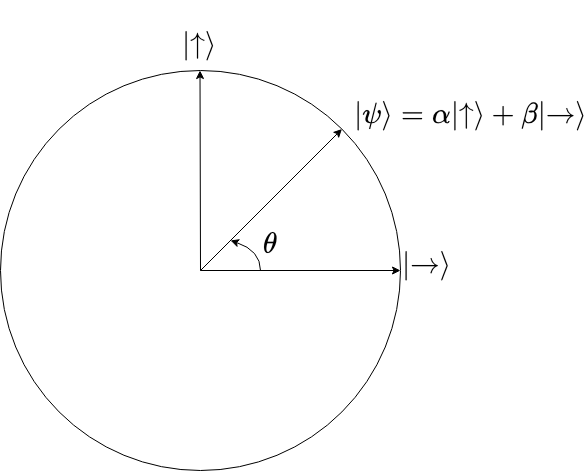
\includegraphics[width=0.45\linewidth]{body/ch2/figs/photon-polarization-circle}
	\caption[Graphical Representation of a Photon Polarisation State.]{A photon can be polarised vertically with probability $|\alpha|^2$ or horizontally with probability $|\beta|^2$. As a consequence of the probability normalisation condition, pure quantum states can be represented graphically on a unit circle as illustrated.}
	\label{fig:photon-polarization-circle}
\end{figure}
If the preferred axis of the polarising gradient is $\ket{\rightarrow}$, the photon is absorbed with a probability of $|\alpha|^2$ and passes through with a probability of $|\beta|^2$. Therefore, the probability that the photon passes through the polariser is the square of the magnitude of the amplitude coefficients in the direction of the preferred axis \cite{Rieffel2011}.

\subsection{Unitary Operations on Quantum States \label{subsec:unitary-ops}}

The analysis of the polarisation state of the quantum system with a single photon explored above can be extended to quantum systems that can be in $N$ different, mutually exclusive classical states. In this case, a quantum state is a superposition of classical states in the form

\begin{align}
	\ket{\psi}	& = \alpha_0 \ket{0} + \alpha_1\ket{1} + ... + \alpha_{N-1} \ket{N-1}
\end{align}
Superposition implies that state $\ket{\psi}$ is in each state $\ket{i}$ with amplitude $\alpha_i$. The vector space $\{\ket{0}, \ket{1}, ..., \ket{N-1}\}$ of states consists of unit vectors that are orthogonal to each other and therefore forms an $N$-dimensional orthonormal basis of a \textit{Hilbert space}, i.e. the vector space of quantum states has an inner product \cite{DeWolf2019}. Thus, a quantum state $\psi$ is a vector in Hilbert space, herein expressed as an $N$-dimensional column vector
\begin{align}
	\ket{\psi}	& = \left(\begin{matrix}
		\alpha_{1} \\
		\alpha_{2} \\
		\vdots \\
		\alpha_{N-1}
	\end{matrix}\right)
\end{align}
with the conjugate transpose
\begin{align}
	\bra{\psi}	& = (\alpha_{0}^{*}, \alpha_{1}^{*}, \hdots, \alpha_{N-1}^{*})
\end{align}
Suppose that the state unit vectors $\ket{0}, \ket{1}, \hdots, \ket{N-1}$ form the orthonormal basis of the Hilbert space $\mathcal{H}_A$, and $\ket{0}, \ket{1}, \hdots, \ket{M-1}$ form an orthonormal basis $\mathcal{H}_B$. The Hilbert spaces $\mathcal{H}_A$ and $\mathcal{H}_B$ can be combined using in a tensor product Hilbert space $\mathcal{H}$, defined as
\begin{align}
	\mathcal{H}	& = \mathcal{H}_A \otimes \mathcal{H}_B 
\end{align}
The output tensor product space has $N\cdot M$ dimensions spanned by the set of states $S_{\mathcal{H}}$, given by
\begin{align}
 S_{\mathcal{H}}	& = \{\ket{a} \otimes \ket{b}\}
\end{align}
where $a \in \{0,1,\hdots, N-1\}$ and $ b \in \{0,1,\hdots, M-1\}$. Thus, any quantum state $\ket{\psi}_{\mathcal{H}}$ in the combined Hilbert space $\mathcal{H}$ can be expressed as the sum
\begin{align}
	\ket{\psi_\mathcal{H}} & = \sum_{i=0}^{N-1}\sum_{j=0}^{M-1} \alpha_{ij} \ket{a_i} \otimes \ket{b_j}
\end{align}
called a \textit{bipartite} quantum state \cite{DeWolf2019}. Although there are higher dimensional tensor products Hilbert space of multiple states, this paper focuses on the operation and simulation of bipartite states.

A linear operation can be performed on a state $\ket{\psi}$ to change it to a different state, $\phi$, Applying the $N \times N$ complex-valued \textit{unitary operation} $U$ on the vector space of the state $\ket{\psi}$ maps it to the space of state $\ket{\phi}$. Formally, a unitary operator is a bounded linear mapping 
\begin{align}
	U: \mathcal{H} \rightarrow \mathcal{H}
\end{align}
on the Hilbert Space $H$ that preserves the norm, and satisfies
\begin{align}
	U^{*}U	& = UU^{*} = I
\end{align}
where $U^{*}$ is the Hermitian adjoint of $U$, and $I$ is the identity operator. The corollary is that a matrix $U$ is \textit{unitary} if 
\begin{align}
	U^{-1}	& = U^{*}
\end{align}
,i.e. if the inverse of $U$ is equal to the complex adjoint of $U$. The linear operator $U$ on the Hilbert space $\mathcal{H}$ defines a Hermitian adjoint operator $U^{*}$ on the space that obeys the rule
\begin{align}
	\braket{Ux, y} & = \braket{x, U^{*}y}
\end{align}
where $\braket{\cdot, \cdot}$ is the inner product on $\mathcal{H}$. Another property of the unitary matrix that can be derived from its definition is that the determinant of $U$ is can be mapped to a unit circle in the complex plane, i.e.
\begin{align}
	|det(U)|	& = 1 
\end{align}
Given an outcome state
\begin{align}
	\phi	& = \beta_0\ket{0} + \beta_1\ket{1} + \hdots + \beta_{N-1}\ket{N-1}
\end{align}
with a probability constraint
\begin{align}
	\sum_{j=0}^{N-1} |\beta_j|^2	& = 1
\end{align}
the unitary transformation $U$ that is applied to $\psi$ can be expressed as the matrix multiplication
\begin{align}
	\ket{\phi}	& = U\ket{\psi}\nonumber\\
	\ket{\phi} & = \left(\begin{matrix}
		u_{11} & u_{12} & \hdots & u_{1N}\\
		u_{21} & u_{22} & \hdots & u_{2N}\\
		\vdots & \vdots & \vdots & \vdots\\
		u_{N1} & u_{N2} & \hdots & u_{NN}
	\end{matrix}\right) 	\left(\begin{matrix}
	\alpha_{1} \\
	\alpha_{2} \\
	\vdots \\
	\alpha_{N-1}
\end{matrix}\right)	\nonumber\\ & = \left(\begin{matrix}
\beta_{1} \\
\beta_{2} \\
\vdots \\
\beta_{N-1}
\end{matrix}\right)
\end{align}
Since the unitary operator is linear and always has an inverse, it follows that operations performed on a quantum state are reversible. That is, the initial state $\ket{\psi}$ can be retrieved by applying the inverse operator $U^{-1}$ to the state $\ket{\phi}$.  

\section{Qubits as Quantum States \label{sec:q-states-qubits}}

\subsection{Qubit Superposition in the Computational Basis}

Quantum computing extends the principles of quantum mechanics to the domain of computation. Unlike a classical bit that can be 0 or 1, but not both at the same time, a \textit{quantum bit} or \textit{qubit}, is a unit of information that can be in a superposition of 0 and 1, corresponding to a quantum state $\ket{\psi}$ of a Hilbert space with two basis states, $\ket{0}$ and $\ket{1}$. 

The basis states are associated with two orthogonal vectors
\begin{align}
	\ket{0} = \left(\begin{matrix}
		1\\
		0
	\end{matrix}\right) &, \ket{1} = \left(\begin{matrix}
	0\\
	1
\end{matrix}\right)
\end{align}
such that, at a given time $t$, a qubit in quantum state $\ket{\psi}$ can be expressed as the superposition
\begin{align}\label{eqn:qstate}
	\ket{\psi}	& = \alpha_0\left(\begin{matrix}
		1\\
		0
	\end{matrix}\right) + \alpha_1\left(\begin{matrix}
	0\\
	1
\end{matrix}\right)
\end{align}
that satisfies the normalisation constraint
\begin{align}
	|\alpha_0|^2 + |\alpha_1| & = 1
\end{align}
This implies that when a qubit in superposition is measured, it collapses with to the state $\ket{0}$ or $\ket{1}$, with a probability of $|\alpha_0|^2$ and $|\alpha_1|^2$, respectively.

\subsection{Qubit Entanglement in the Computational Basis\label{subsec:qubit-entanglement}}
Quantum systems of multiple qubits exist in two-dimensional complex Hilbert space as described in section \ref{subsec:q-states} for quantum states of $N$ particles. The $N$-dimensional tensor product space of the system contains a set of basis states with a cardinality of $2^{N}$, i.e. a system with $n$ qubits has $2^n$ basis states, each of the form
\begin{align}
	\ket{q_1}\otimes\ket{q_2}\otimes\hdots\otimes\ket{q_n}
\end{align} 
with $q_i\in \{0,1\}$. In this paper, basis states are abbreviated as $\ket{q_1 q_2 q_3 \hdots q_n}$ or written in decimal form as $\ket{1}, ~\ket{2}, \hdots, \ket{2^n -1}$, depending on the computation. A quantum system with multiple qubits is referred to as a \textit{quantum register} of $n$ qubits and is considered to be in any superposition of the $n$ states represented in decimal form as
\begin{align}\label{eqn:multiple-qubit-state}
	\ket{\psi_{qr}} & = \alpha_{0}\ket{0} + \alpha_{1}\ket{1} + \alpha_2 \ket{2} + \cdots + \alpha_{2^n - 1}\ket{2^{n-1}}
\end{align}  
for
\begin{align}
	 \sum_{i=0}^{2^n - 1} |\alpha_i|^2 & = 1 	
\end{align}
Composite systems consist of two or more quantum subsystems. Statistical ensembles of pure quantum subsystem spaces show non-classical correlations between basis states, known as \textit{quantum entanglement}.  Qubits in composite quantum systems can leverage quantum \textit{entanglement} to facilitate linear operations and classical communications (LOCC). Formally, a pure quantum state $\ket{\psi}$ is said to be entangled if it is not \textit{separable}. A separable pure state $\ket{\xi}$, in a tensor product Hilbert space $\mathcal{H}_{nm} = \mathcal{H}_n \otimes \mathcal{H}_m$, can be written as the tensor product of states $\psi~\in~\mathcal{H}_n$ and $\phi~\in~\mathcal{H}_m$, i.e.
\begin{align}
	\ket{\xi}	& = \ket{\psi}\otimes\ket{\phi}
\end{align}
Consider the pure bipartite state
\begin{align}
	\ket{\psi^+}	& = \frac{1}{\sqrt{2}}\ket{00}+\frac{1}{\sqrt{2}}\ket{11}
\end{align}
from the tensor product space $\mathcal{H}_{22} = \mathcal{H}_{2}\otimes\mathcal{H}_2$. It can be shown that this bipartite state $\ket{\psi}^+$, known as an EPR pair, is indeed entangled. Let
\begin{align}
	\ket{\psi_1}	& = \alpha\ket{0} + \beta\ket{1}\nonumber\\
	\ket{\psi_2} 	& = \gamma\ket{0} + \delta\ket{1}\nonumber
\end{align} 
be pure states from the two-dimensional Hilbert space where
\begin{align}
	|\alpha|^2 + |\beta|^2 & = 1\nonumber\\
	|\gamma|^2 + |\delta|^2 & = 1\nonumber
\end{align}
If the state $\ket{\psi}^+$ is separable, it can be written as
\begin{align}
	\ket{\psi}^+	& = \ket{\psi_1}	\otimes		\ket{\psi_2}\nonumber\\
					& = (\alpha\ket{0} + \beta\ket{1})\otimes(\gamma\ket{0} + \delta\ket{1})\nonumber
\end{align}
From the property of distributivity of the tensor product and the assumption of separability, the bipartite state $\psi^{+}$ the product above can be expanded to
\begin{align}
	\ket{\psi}^+	& = \frac{1}{\sqrt{2}}\ket{00}+\frac{1}{\sqrt{2}}\ket{11}\nonumber\\
					& = \alpha\gamma\ket{00} + \alpha\delta\ket{01} + \beta\gamma\ket{10} + \beta\delta\ket{11}\nonumber 
\end{align}
For the assumption of separability to hold true, the state amplitudes must satisfy
\begin{align}
	\alpha\delta&=\beta\gamma=0\nonumber\\
	\alpha\gamma&=\beta\delta=\frac{1}{\sqrt{2}}\nonumber
\end{align}
Since there are no values such that these statements are true, it must be that 
\begin{align}
	\ket{\psi}^+	& \neq \ket{\psi_1}\otimes\ket{\psi_2}\nonumber
\end{align}
Hence, the pure state $\ket{\psi^+}$ is entangled \cite{Kurzyk2012}. Similarly, it can be shown that the state $\ket{\psi^-}$ defined by
\begin{align}
	\ket{\psi^-}	& =  \frac{1}{\sqrt{2}}\ket{00}-\frac{1}{\sqrt{2}}\ket{00}\nonumber
\end{align}
is an entangled state.   Initially, both $\ket{\psi_1}$ and $\ket{\psi_2}$ are in a superposition of the $\ket{0}$ and $\ket{1}$ basis states. The state of the qubit collapses to $\ket{00}$ when state $\ket{\psi_1}$ is measured and $\ket{0}$ is observed. Therefore, an observation of the eigenstate $\ket{\psi_1}$ is correlated to the eigenstate $\ket{\psi_2}$ of the second qubit that was not observed.
The states $\ket{\psi^+}$ and $\ket{\psi^-}$ belong to a set of four orthogonal eigenvectors of entangled states, namely
\begin{align}
	\ket{\psi^\pm} & = \frac{1}{\sqrt{2}}\ket{00} \pm \frac{1}{\sqrt{2}}\ket{11}\\
	\ket{\phi^\pm} & = \frac{1}{\sqrt{2}}\ket{01} \pm \frac{1}{\sqrt{2}}\ket{10}
\end{align}
Entanglement in bipartite state quantum systems can be exploited using non-local quantum unitary operations. These operations are independent of the distance between entangled qubits, since information about one state in an entangled 2-qubit system simultaneously reveals information about an associated, non-classically correlated state.

The degree of qubit entanglement is quantified by the \textit{Schmidt number} whose logarithm corresponds to the zero-error entanglement cost of generating a given quantum state using LOCC \cite{Gupta2020}. Quantum information theory also uses \textit{von Neumann entropy} to quantify the extent of entangle of qubits. This is because for an system of entangled states, von Neumann entropy of a joint Hilbert space $\mathcal{H}_{nm}$ can be smaller than the entropy of its subsystems. To define von Neumann entropy, a density operator $\rho$ is assigned to a quantum system with pure state and is given by
\begin{align}
	\rho	& = \ket{\psi}\bra{\psi}
\end{align}
A mixed state is a statistical ensemble of density operators of pure states, where each density operator $\rho$ is a Hermitian projection operator which satisfies $\rho^2 = \rho$. The von Neumann entropy $\mathcal{E}$ is then defined as
\begin{align}
	\mathcal{E}(\rho)	& = -\text{tr}(\rho \log \rho)
\end{align}
The von Neumann entropy of a pure quantum state is equal to 0, and the entropy of a maximally mixed state is equal to
\begin{align}
	\mathcal{E}(\rho)	& = - \sum_{i=0}^{n} \frac{1}{n} \log \frac{1}{n} = \log n
\end{align}
Similarly, it can be shown that if $\rho_n$, $\rho_m$ and $\rho_{nm}$ are the density operators of quantum systems $\mathcal{H}_n$, $\mathcal{H}_m$, and composite system $\mathcal{H}_nm$, then the joint von Neumann entropy of the system must satisfy
\begin{align}
	\mathcal{E}(\rho_n, \rho_m) & = \mathcal{E}(\rho_{nm})
\end{align}
More intuitively, the von Neumann entropy is a measure of the stability of a measurement on a quantum system. A measure of entanglement $E$ must satisfy LOCC monoticity in that it cannot increase under LOCC operations. That is to say, when all operations are performed locally on the respective subsystem and information between subsystems is transmitted using classical communication channels, the measure of entanglement $E$ must be invariant under local unitary operations. Other measures, such as the \textit{entanglement cost}, give information about how expensive it is to create an entangled state with density operator $\rho$, using LOCC operations in a bipartite entangled state \cite{Kurzyk2012}. For pure states, von Neumann entropy suffices as an entanglement measure.

\section{Quantum Gates and Quantum Circuits \label{sec:q-gates+q-circuits}}

Complex operations on classical computers are completed using primitive logic gates such as \texttt{NOT}, \texttt{AND}, \texttt{OR}, \texttt{NOR}, \texttt{NAND} and \texttt{XNOR} gates. Analogously, quantum state transformations on an $n$ qubit system can be executed by an application simple unitary operations on one- and two-qubit quantum systems. Quantum state transformations that act on a finite number of qubits are called \textit{quantum gates}. A collection or sequence of quantum gates is referred to as a \textit{quantum circuit}. 

\subsection{Bloch Sphere Representation of Qubits \label{subsec:bloch-sphere}}

The quantum state ${\ket{\psi}}$ in equation \ref{eqn:qstate} with complex amplitudes $\alpha$ and $\beta$, can be written in the polar form 
\begin{align}\label{eqn:qstatephase}
	\ket{\psi}	& = r_{\alpha}e^{i\theta_\alpha}\ket{0} + r_{\beta}e^{i\theta_\beta}\ket{1}
\end{align}
to expose the phase of a qubit. The \textit{relative phase} $\phi_r$ of the system is defined as the angle between the state vectors in a Hilbert space. More concisely,
\begin{align}
	\phi_r	& = \theta_\alpha - \theta_\beta
\end{align}
Changing the relative phase of a qubit is equivalent to performing a rotation of the state vector in Hilbert space. Unlike the relative phase, \textit{global phase} $\gamma_g$ is arbitrary and does not have any physical meaning, therefore, multiplying the state $\ket{\psi}$ by an arbitrary global phase does not change the state in a meaningful manner, i.e.
\begin{align}
	\ket{\psi}	& = e^{i\gamma_g}\ket{\psi}
\end{align}
This property of the global phase also implies that multiplication of the wave function represented by $\alpha\ket{0}$ with a global phase rotation does not have an effect on the state, therefore
\begin{align}
	\ket{\psi} & = \alpha \ket{0} + e^{i\gamma_g}{\beta}\ket{1}\nonumber
\end{align}
Let $\gamma_g = \phi_r$ be the global phase. From the property of the global phase, the quantum state $\ket{\psi}$ can be expressed such that the only unknown is the relative phase $\phi_r$,
\begin{align}
	\ket{\phi}	& = \alpha\ket{0} + e^{i\phi_r}\beta\ket{1}
\end{align}
The normalisation constraint on the state requires that
\begin{align}
	|\alpha|^2+|\beta|^2&=1
\end{align}	
which represents an unit circle in the complex plane. By setting 
\begin{align}
	\alpha	& = \cos\theta\\
	\beta	& = \sin\theta
\end{align}
where $\theta \in \mathbb{R}$ is the \textit{absolute phase}, the normalisation constraint holds and a qubit can be represented using a \textit{Bloch sphere} diagram which maps the state vector to a spherical 3D Hilbert subspace to represent information about the relative phase of the state and the argument of the amplitudes as illustrated in figure \ref{fig:blochsphere}. 
\begin{figure}
	\centering
	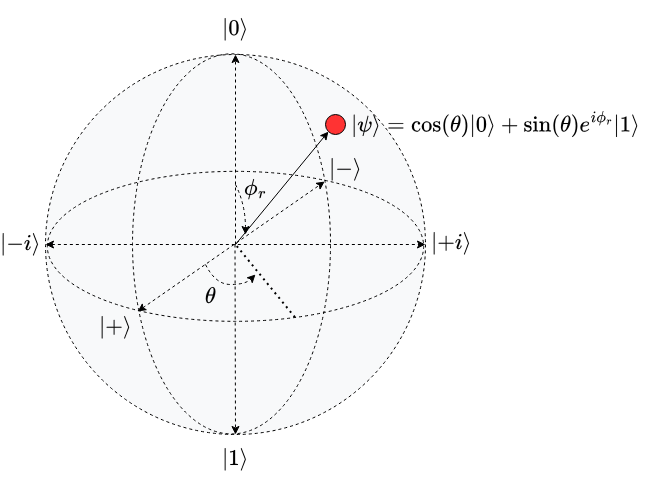
\includegraphics[width=0.80\linewidth]{body/ch2/figs/blochsphere}
	\caption[Bloch sphere diagram representing the quantum state of a qubit as a vector in Hilbert space.]{Showing a Bloch sphere diagram where relative phase is mapped to the vertical rotation around the $xy$-plane and $\theta$ corresponds the angle of the horizontal rotation of the qubit around the $\hat{z}$-axis.}
	\label{fig:blochsphere}
\end{figure}
The Bloch sphere is centred at the origin with a radius of 1. The absolute phase $\theta$ is taken with respect to the $\hat{z}$-axis corresponding to the orthogonal basis vectors, $\ket{0}$ and $\ket{1}$, of the state space. The relative phase $\phi$ is considered with respect to the $\hat{x}$-axis. Generally, each axis of the 3D plane represents two counter states. The states on the $\hat{z}$-axis correspond to the basis vectors,
\begin{align}
	\ket{0}	= \left(\begin{matrix}
		1\\
		0
	\end{matrix}\right) &, 	\ket{1}	= \left(\begin{matrix}
	0\\
	1
\end{matrix}\right)\nonumber
\end{align}
The $\hat{x}$-axis represents the EPR pair, or Bell states, namely,
\begin{align}
		\ket{+}	& = 
		\frac{1}{\sqrt{2}}\left(\begin{matrix}
										1\\
										0
								\end{matrix}\right) + 
		\frac{1}{\sqrt{2}}\left(\begin{matrix}
										0\\
										1
								\end{matrix}\right)\nonumber\\
		\ket{-}	& = 
		\frac{1}{\sqrt{2}}\left(\begin{matrix}
										1\\
										0
								\end{matrix}\right) - 
		\frac{1}{\sqrt{2}}\left(\begin{matrix}
										0\\
										1
								\end{matrix}\right)\nonumber
\end{align}
Similarly, the $\hat{y}$-axis represents the imaginary part of the state vector, or mathematically,
\begin{align}
	\ket{+i}	& = 
	\frac{1}{\sqrt{2}}\left(\begin{matrix}
		1\\
		0
	\end{matrix}\right) + 
	\frac{i}{\sqrt{2}}\left(\begin{matrix}
		0\\
		1
	\end{matrix}\right)\nonumber\\
	\ket{-i}	& = 
	\frac{1}{\sqrt{2}}\left(\begin{matrix}
		1\\
		0
	\end{matrix}\right) - 
	\frac{i}{\sqrt{2}}\left(\begin{matrix}
		0\\
		1
	\end{matrix}\right)\nonumber
\end{align}
Every point on the surface of a Bloch sphere represents a quantum state. This makes Bloch sphere diagrams a very powerful tool for representing quantum gate transformations applied to a qubit.

\subsection{Single-Qubit Quantum Gates\label{subsec:single-q-gates}}

Applications of quantum information processing employs single qubit gates as more of a mathematical abstraction compared to realisable classical logic gates. Quantum gates are not always physically but are extensively used in analysing quantum computing algorithms. From a mathematical point of view, quantum gates are unitary transformations on a small number of qubits. Typically, quantum gates work with up to 3 qubits. 

Single qubit gates correspond to unitary operations known as \textit{Pauli} matrices, I, X, Y, and Z. The Pauli-\texttt{X} gate is analogous to a classical \texttt{NOT} gate in that it performs a qubit flip transformation. For example, given an initial observation of the state $\psi$ which is specified by normalised amplitudes $\alpha$ and $\beta$, the \texttt{X} gate acts linearly to interchange the amplitude of the coefficients that define the superposition by the transformation
\begin{align}
	\texttt{X}: & \ket{\psi}\rightarrow\ket{\psi'}
\end{align}
for 
\begin{align}
	\ket{\psi} & = \alpha\ket{0} + \beta\ket{1}\nonumber\\
	\ket{\psi'} & = \alpha\ket{1} + \beta\ket{0}
\end{align}
The unitary matrix representing the X gate transformation is written as
\begin{align}
	X	& = \left(\begin{matrix}
		0 & 1\\
		1 & 0
	\end{matrix}\right)
\end{align}
Thus, given a qubit in Hilbert space $H_2$ with normalised amplitudes $\alpha$ and $\beta$, the output of the \texttt{X} gate unitary operator is
\begin{align}
	X	\left(\begin{matrix}
	\alpha\\
	\beta
\end{matrix}\right) & = 
\left(\begin{matrix}
	\beta\\
	\alpha
\end{matrix}\right)
\end{align}
This transformation can also be illustrated on a Bloch sphere as shown in figure \ref{fig:xgatebloch} where the initially measured state of the qubit, $\ket{\psi_1}$, is rotated around the $\hat{x}$-axis by $\pi~\si{\radian}$ to obtain $\ket{\psi_2}$. 
\begin{figure}[ht!]
	\centering
	\begin{subfigure}[b]{0.28\textwidth}
		\centering
		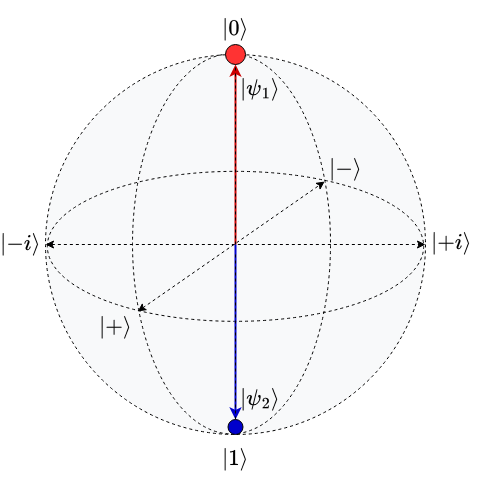
\includegraphics[width=0.9\textwidth]{body/ch2/figs/x-gate}
		\caption{Pauli-\texttt{X} gate.}
		\label{fig:xgatebloch}
	\end{subfigure}
	\hfill
	\begin{subfigure}[b]{0.28\textwidth}
		\centering
		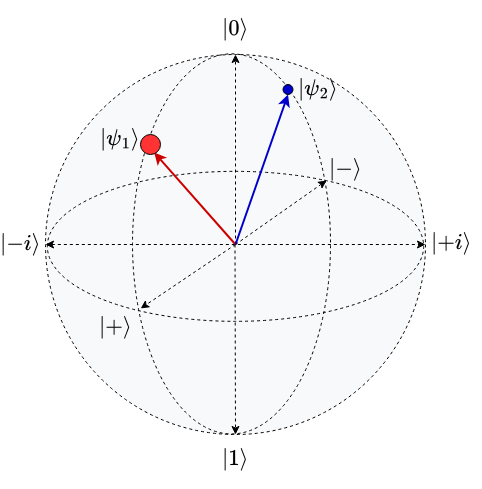
\includegraphics[width=0.9\textwidth]{body/ch2/figs/z-gate}
		\caption{Pauli-\texttt{Z} gate.}
		\label{fig:zgatebloch}
	\end{subfigure}
	\hfill
	\begin{subfigure}[b]{0.28\textwidth}
		\centering
		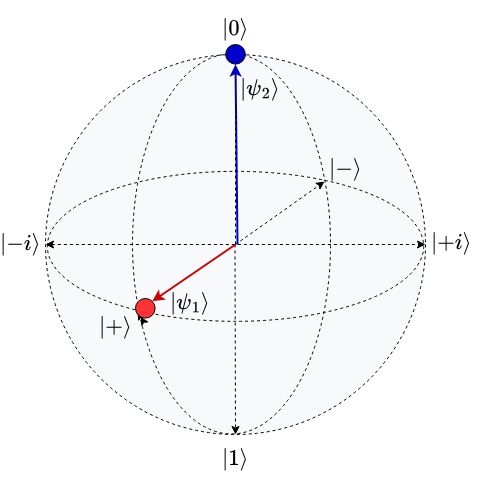
\includegraphics[width=0.9\textwidth]{body/ch2/figs/hadamard-gate}
		\caption{Hadamard (\texttt{H}) gate.}
		\label{fig:hadamardbloch}
	\end{subfigure}
	\caption{Three Bloch spheres representing important single-qubit quantum gate operations. The initial state is in red and the final measured state is blue. The \texttt{X} gate is analogous to a classical \texttt{NOT} gate and the \texttt{Z} gate changes the phase of the qubit.}
	\label{fig:qgates}
\end{figure}

Since the quantum gate is a unitary operator, it maintains the condition of normalisation on the Hilbert space \cite{Nielsen2010}. Other Pauli gate matrices are expressed in equation \ref{eqn:pauligates} where it can be shown that for each unitary matrix $U$, $UU^\dagger=I$, where $U^\dagger$ is the adjoint of $U$. This implies that the identity matrix $I$, operates in a manner that is analogous to a classical circuit buffer which has the same bit at input and output. Applying the an identity gate is equivalent to measuring the same state at the start and end of a computation, the input state of the quantum system is the same as the output state. 
\begin{align}\label{eqn:pauligates}
	I=\left(\begin{matrix}
		1	& 0\\
		0	& 1
	\end{matrix}\right)&;~Y=\left(\begin{matrix}
	0	& -i\\
	i	& 0
\end{matrix}\right)\nonumber\\
Z=\left(\begin{matrix}
1	& 0\\
0	& -1
\end{matrix}\right)&;~H=\frac{1}{\sqrt{2}}\left(\begin{matrix}
1	& 1\\
1	& -1
\end{matrix}\right)
\end{align}
The \texttt{X} gate is one of three physically realisable single-qubit gates that are considered in this research. The other two gates that are of significance to quantum information processing are the Pauli-$Z$ gate and the \textit{Hadamard} gate \texttt{H} - illustrated using Bloch diagrams as shown in figure \ref{fig:zgatebloch} and \ref{fig:hadamardbloch}, respectively. 

Equation \ref{eqn:pauligates} shows that the $Y$ gate performs rotations through the $\hat{y}$-axis which corresponds to the complex plane and is therefore not physically realisable. The \texttt{Z} gate is a special case of the \textit{phase gate},
\begin{align}
	R_\phi	& = \left(\begin{matrix}
		1	& 0\\
		0	& e^{i\phi}
	\end{matrix}\right)
\end{align}
which rotates the state vector of a qubit through the $\hat{z}$-axis by $\phi=\pi~\si{\radian}$, effectively negating the amplitude of the $\ket{1}$ basis state and leaving the $\ket{0}$ basis state unchanged. The Hadamard gate \texttt{H} rotates the qubit by $\pi/2~\si{\radian}$ through the $\hat{y}$-axis and by $\pi~\si{\radian}$ in the $\hat{x}$-axis.  

This implies that, given an initial state $\ket{0}$ to which the Hadamard gate is applied, there is an equal probability of observing $\ket{0}$ or $\ket{1}$ \cite{DeWolf2019}. When a Hadamard gate is applied to the $\ket{+}$ state, the output is derived from
\begin{align}
	H\ket{+} & = H\left[\frac{1}{\sqrt{2}}\left(\begin{matrix}
						1\\0
	\end{matrix}\right) + \frac{1}{\sqrt{2}}\left(\begin{matrix}
	0\\1
\end{matrix}\right)\right]\nonumber\\
& = \frac{1}{\sqrt{2}}H\left(\begin{matrix}
	1\\0
\end{matrix}\right) + \frac{1}{\sqrt{2}}H\left(\begin{matrix}
	0\\1
\end{matrix}\right)\nonumber\\
& = \frac{1}{2}\left(\begin{matrix}
	1\\0
\end{matrix}\right) + \frac{1}{2}\left(\begin{matrix}
	0\\1
\end{matrix}\right) + \frac{1}{2}\left(\begin{matrix}
1\\0
\end{matrix}\right)  \frac{1}{2}\left(\begin{matrix}
0\\1
\end{matrix}\right)\nonumber
\end{align}
which gives the state $\ket{0}$. This derivation of the Hadamard operation exposes the phenomenon of \textit{interference} that qubits experience due to their wave nature. This occurs when the $\ket{1}$ and $-\ket{1}$ states cancel each other out, corresponding to an overlap in the peaks and troughs of the qubit waveforms that are in a superposition of states.

When simulating single-qubit quantum gates, the Hadamard gate is off particular interest since it increases the entropy of the classical computer running the simulation. For this reason, models of the Hadamard gate on the FPGA were expected to use more logic and slices than other single-input quantum gates. Other single-qubit gates can be performed using LUT-multipliers and simple combinational logic operations. 
 
\subsection{Multiple-Qubit Gates\label{subsec:multiple-q-gates}}
Multiple-qubit gates can be realised by performing a sequence of single-qubit gate transformations. Constructing a multiple-qubit gate from two single-qubit systems given by matrix $U$ and matrix $V$ equivalent to taking the tensor product of the matrices, i.e. $U\otimes V$. In some cases, multiple-qubit gates can transform the system such that qubits become entangled. Generally, these type of gates cannot be decomposed into a tensor product of single-bit transformation. An example of a 2-qubit gate is the \textit{controlled}-\texttt{NOT} (\texttt{CNOT}) gate which is defined as the sum of tensor products of the identity matrix \texttt{I} and the \texttt{X} gate with the standard basis inputs $\ket{0}$ and $\ket{1}$, i.e.,
\begin{align}\label{eqn:cnotdef}
	\texttt{CNOT}	&= \ket{0}\bra{0}\otimes I + \ket{1}\bra{1}\otimes X
\end{align}
Equivalently, the unitary matrix representation of the \texttt{CNOT} gate is
\begin{align}\label{eqn:cnotmatrix}
	\texttt{CNOT}	& = \left(\begin{matrix}
		1 & 0  & 0 & 0\\
		0 & 1  & 0 & 0\\
		0 & 0  & 0 & 1 \\
		0 & 0  & 1 & 0
	\end{matrix}\right)
\end{align}
Given a standard basis input, the \texttt{CNOT} gate has four possible outputs, namely,
\begin{align}
	\texttt{CNOT}~~: & \begin{cases}
		\ket{00} \rightarrow \ket{00}\\
		\ket{01} \rightarrow \ket{01}\\
		\ket{10} \rightarrow \ket{11}\\
		\ket{11} \rightarrow \ket{10}	
	\end{cases}
\end{align}
The $\texttt{CNOT}$ gate is particularly important for applications in quantum information processing due to its capability to change the entanglement between input qubits \cite{Rieffel2011}. For example, given the separable 2-qubit input state $\ket{\psi_1}$ where  
\begin{align}
	\ket{\psi_1}	& = \frac{1}{\sqrt{2}}\left(\ket{0} + \ket{1}\right)\otimes\ket{0}
\end{align}
the \texttt{CNOT} gate converts unentangled input state to an entangled Bell state
\begin{align}
	\ket{\psi_2} 	& = \frac{1}{\sqrt{2}}\left(\ket{00} + \ket{11}\right)\nonumber
\end{align}
The generalised \texttt{CNOT} gate consists of gates that perform a single-qubit transformation $Q$ on the second qubit in the input when the first input is the basis state $\ket{1}$ and leave it unchanged when the first input is $\ket{0}$. The first input is called the \textit{control qubit} and the second qubit is called the \textit{target qubit}. Formally, the generalised \text{CNOT} gate can be expressed as
\begin{align}
	\Lambda Q	& = \ket{0}\bra{0}\otimes I + \ket{1}\bra{1}\otimes Q
\end{align}
where $Q$ is a $2\times2$ matrix. Thus, the $4\times4$ matrix representation of the generalised \texttt{CNOT} gate is
\begin{align}\label{eqn:generic-cnot}
	\Lambda Q	& = \left(\begin{matrix}
						1	&0	&0	&0\\
						0	&1	&0	&0\\
						0	&0	&q_{11}	&q_{12}\\
						0	&0	&q_{21}	&q_{22}
					\end{matrix}\right)
\end{align}
where each $q_{ij}$, for $i = 1,2$ and $j=1,2$, is an element of the single-qubit gate $Q$. The graphical representation of the generalised \texttt{CNOT} gate and the special case of the \texttt{CNOT} which uses the $X$ gate is shown in figure \ref{fig:cnotDiagram}.
\begin{figure}
	\centering
	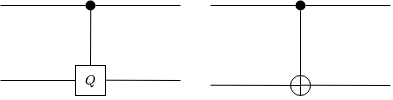
\includegraphics[width=0.75\linewidth]{body/ch2/figs/cnot-diagram}
	\caption[Generalised \texttt{CNOT} gate and the $\Lambda X$ \texttt{CNOT} gate.]{The $\Lambda X$ gate is a 2-qubit gate which is a special case of the generalised 2-qubit $\Lambda Q$ \texttt{CNOT} gate.}
	\label{fig:cnotDiagram}
\end{figure}
Note that the control qubit of the \texttt{CNOT} gate does not change and the target qubit changes depending on the state of the control qubit. This operation is analogous to the operation of the \texttt{XOR} gate, since the unitary transformation can also be expressed algebraically as
\begin{align}
	\texttt{CNOT}: & \ket{A,B} \rightarrow \ket{A, B\oplus A }
\end{align}
where $\oplus$ represents the direct sum of the basis sets $A$ and $B$ that produces a vector space with basis $A\cup B$.

Emulations of controlled gate operations require more area on FPGA hardware than single-qubit gates since they operate on two qubits simultaneously to and require dense matrix operations for large $n$. Additionally, the output of a controlled gate is an entangled state which increases the amount of storage required to represent quantum states on the FPGA hardware. Therefore, the number of controlled gates in a quantum circuit was expected to directly influence the overall performance of the simulation. 

\subsection{Quantum Circuits \label{subsec:q-circuits}}
Illustrations of the \texttt{CNOT} gate as shown in figure \ref{fig:cnotDiagram} form an essential part of representing and interpreting quantum computations. A sequence of quantum gates forms a \textit{quantum gate array}, also known as a \textit{quantum circuit}. Quantum circuits are a universal language for describing complex quantum computations \cite.  In a quantum circuit, single-qubit gates are represented using block diagram notation as depicted in figure \ref{fig:gatecircuitcomponents}. In 1995, Barenco et al. proved that arbitrary quantum circuits can be expressed by compositions of a set of single-qubit gates and \texttt{CNOT} gates \cite{barenco1995elementary}. Furthermore, since there are infinitely many $2\times2$ unitary matrices, there are also infinitely many single-qubit gates and quantum circuits. 
\begin{figure}[!ht]
	\centering
	
\includegraphics[width=0.85\linewidth]{body/ch2/figs/single-qubit-components}
	\caption[Showing the circuit representation of quantum $X$, $Z$ and $H$ gates.]{Quantum circuit gate component representations of the Pauli-$X$, Pauli-$Z$ and $H$ single-qubit logic gates.}
	\label{fig:gatecircuitcomponents}
\end{figure}
In quantum circuit representations, time progresses from the input of the quantum circuit on the left, to the right which terminates in a measurement of the output state. Each line in the quantum circuit represents a wire, which in turn, represents the passage of time from left to right or a qubit of information as it is translated in Hilbert space. By convention, it is assumed that the multiple-qubit input to a circuit is the state consisting of a sequence of $\ket{0}$ basis states. It is crucial to note that the final state of an input qubit cannot be determined by only looking at the wire corresponding to that qubit. For example, from the circuit in figure \ref{fig:hadamard2circuit}, 
\begin{figure}[!ht]
	\centering
	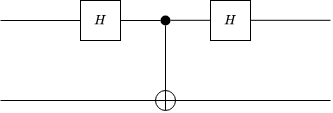
\includegraphics[width=0.75\linewidth]{body/ch2/figs/q-circuit-caution}
	\caption[The output of a qubit cannot be accurately determined by looking at a single line in a quantum circuit.]{Demonstrating a quantum circuit that consists of two series $H$ gates on the control line of the $\Lambda X$ gate.}
	\label{fig:hadamard2circuit}
\end{figure}
it might appear that the first qubit's state would remain the same since $H^2 = I$, however, given the input state $\ket{00}$, the state of the output is defined by the unitary transformation
\begin{align}
	U: & \ket{00} \rightarrow \frac{1}{2}\left(\ket{00} + \ket{10} + \ket{01} - \ket{11}\right) \nonumber
\end{align}
which is not obvious by focusing on the control line of the circuit \cite{Rieffel2011}. Figure \ref{fig:swapcircuit} shows another example of a quantum circuit known as a \textit{swap gate} which contains three \texttt{CNOT} gates. Since the \texttt{swap} gate uses \texttt{CNOT} gates, it follows a sequence of transformations on a basis state $\ket{\psi_a, \psi_b}$ that involves direct sums of vector states that produces an output where the qubit states are interchanged. The \texttt{swap} gate uses both qubits as the control to perform the operation
\begin{align}
	\ket{\psi_a, \psi_b}	&\rightarrow \ket{\psi_a, \psi_a\oplus \psi_b}\nonumber\\
				&\rightarrow \ket{\psi_a\oplus (\psi_a\oplus \psi_b), \psi_a\oplus \psi_b}\nonumber\\
				& = \ket{\psi_b, \psi_a\oplus\psi_b}\nonumber\\
				& \rightarrow \ket{\psi_b, (\psi_a\oplus\psi_b)\oplus\psi_b}\nonumber\\
				& = \ket{\psi_b, \psi_a}
\end{align}
The \texttt{swap} gate is also equivalent to applying the transformation $U$, given by,
\begin{align}
	U: & \ket{\psi_a}\bra{\psi_a}\otimes X	+ \ket{\psi_b}\bra{\psi_b} \otimes X
\end{align}
which applies a tensor product of the Pauli-$X$ gate to each qubit in the system. 
\begin{figure}[!ht]
	\centering
	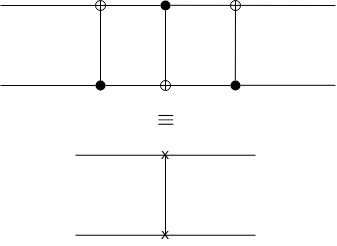
\includegraphics[scale=0.55]{body/ch2/figs/swap-circuit}
	\caption[Swap gate interchanges input qubits in a 2-qubit system.]{Quantum circuit of a \texttt{swap} gate that interchanges the input state from $\ket{\psi_a,\psi_b}$ to $\ket{\psi_b,\psi_a}$.}
	\label{fig:swapcircuit}
\end{figure}
Quantum circuits are said to be \textit{acyclic} in that feedback from one part of the circuit to another is prohibited \cite{Rieffel2011}. This is contrary to classical electronic circuits which employ feedback to control the stability of classical systems. Another contradiction between quantum circuits and classical circuits is that quantum circuit wires cannot be joined together to perform an operation that is analogous to a classical \texttt{OR} gate operation. Additionally, most quantum circuit operations are reversible since they use unitary operations, however, duplication of qubit states is prohibited according to the \textit{no-cloning theorem}, which implies that copy operations at the output of a quantum circuit are prohibited.  

Quantum circuit outputs are measured to collapse the single qubit state $\ket{\psi}$ with basis states $\ket{0}$ and $\ket{1}$ to a classical bit $\sigma$ where the probability of obtaining $0$ is $|\alpha|^2$ and the probability of obtaining 1 is $|\beta|^2$, such that the normalisation condition is satisfied. The symbol for a measurement in a quantum circuit is shown in figure \ref{fig:measurement-symbol} where $\sigma$ is represented by a double-line wire. 
\begin{figure}[!ht]
	\centering
	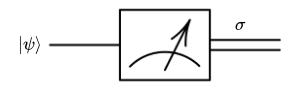
\includegraphics[width=0.70\linewidth]{body/ch2/figs/measurement-symbol}
	\caption[Quantum circuit measurement symbol.]{Quantum circuit measurement symbol.}
	\label{fig:measurement-symbol}
\end{figure}
A measurement on a multidimensional qubit (sometimes referred to as a "qudit") collapses the superposition of states to a single classical $n$-bit configuration that is chosen randomly with probability that satisfies the normalisation condition on the amplitudes of each state. A measurement can also be viewed as an interface that converts quantum information to classical information. By the no-cloning theorem, measurements of the output of a quantum circuit are irreversible as the quantum information is destroyed when the superposition of states collapses into a single classical bit or strings of classical bits. One way around the no-cloning theorem is to implement teleportation and quantum error-correction in which information about the quantum state being measure is concealed. 
 
\textit{Circuit depth} refers to the count of time steps from the initialisation of the qubits to the final measurement taken. In determining the circuit depth, all gates executed in parallel count as one time step, including cases where the execution times of each gate are significantly different \cite{de2021reducing}. Analogously, the critical path of FPGA designs refers to the longest sequence of logic gates that data must pass through and the latency of the digital circuit. In designing the simulation of quantum gates on FPGA, the aim is to reduce the critical path by parallelising operations involving multiple qubit gates such as the controlled gate. For FPGAs however, the critical path includes pipeline registers for storing quantum state evolutions during the execution of a quantum circuits simulations.

\subsection{Theoretical Framework for Quantum Algorithms \label{subsec:qft}}

In quantum computing, \textit{quantum algorithms} are executed using quantum circuits. During the proposal of elementary gates for quantum computing, Barenco et al. suggested that most quantum algorithms can be decomposed into a combination of single-qubit gates such as the previously described Pauli gates and two-qubit \texttt{CNOT} gates represented as $2^n \times 2^n$ dense matrices \cite{barenco1995elementary}. Applying unitary quantum gates to qubits in a quantum circuit transforms the $2^n$ complex entries of the $n$-qubit state vector, corresponding to a multiplication of the qubit state vector with the unitary matrix of the quantum gate \cite{li2019tackling}. To emulate a quantum computer on available classical computers, H\"{a}ner et al. suggest that instead of simulating the vast number of quantum gates required for a quantum computation, one can perform the classical function directly for each computational basis state \cite{haner2016high}. Developed here is the formalism of the Quantum Fourier Transform (QFT) which is the primary quantum circuit in Shor's quantum factoring algorithm and other quantum algorithms. The mathematical formalism of the \textit{quantum search algorithm}, also known as \textit{Grover's search algorithm}, is also considered in this section. Understanding of these algorithms is critical in the emulation of the quantum computer on FPGA. 

\subsubsection{Quantum Fourier Transform \label{subsubsec:qft}}

In the analysis of linear time-dependent classical systems, the Fourier transform is harnessed as a reversible tool that transforms a signal from the time domain to the frequency domain and vice versa. In the discrete time domain, the Fast Fourier transform (FFT) is performed to reduce the computational complexity by decomposing the Discrete Fourier transform (DFT) of a signal into two half-point transforms. In quantum computing, the QFT is the quantum counterpart of classical DFT algorithms. A 3-qubit QFT circuit demonstrated by Nielsen and Chuang, uses a sequence of \texttt{H} gates, $\texttt{R}_\phi$ phase gates, and a special case of the phase gate known as the \texttt{T} gate which rotates a state vector by $\phi=\pi/8~\si{\radian}$. For an $n$-qubit system, a total of $n(n+1)/2+n/2$ gates are required to perform the QFT \cite{Nielsen2010}. Since each quantum gate transformation involves matrix multiplication and vector addition operations, simulations of the QFT require intensive computational resources. This high performance capabilities of FPGAs makes them suitable for performing quantum experiments using a simulation of the QFT. 
\begin{figure}[!ht]
	\centering
	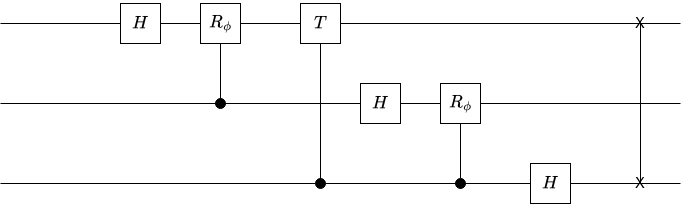
\includegraphics[width=1.0\linewidth]{body/ch3/figs/nielsen-qft}
	\caption[Nielsen 3-qubit QFT.]{An explicit quantum circuit for the 3-qubit Quantum Fourier Transform which uses the Hadamard gate, $H$, phase gate, $R_\phi$, and the $\pi/8$ gate, $T$.}
	\label{fig:nielsen-qft}
\end{figure}
Formally, the QFT on the basis $\ket{0}, \ket{1}, ...,\ket{N-1}$ is defined to be a linear operator with the following transformation on the vector space, 
\begin{align}\label{eqn:qft}
	\ket{j}	& \rightarrowtail \frac{1}{\sqrt{N}} \sum_{k=0}^{N-1} e^{2\pi i j k/N}\ket{k}
\end{align}
which is a unitary transformation that can be implemented using a quantum computer \cite{Nielsen2010}. Note the state $\ket{j}$ can be written in the binary representation $j = j_1j_2...j_n$. It can be shown that the QFT is a unitary transformation by expanding the definition. Let $N=2^n$, where $n$ is an integer, and let the basis $\ket{0},...,\ket{2^n - 1}$ be the computational basis for an $n$ qubit quantum computer \cite{Nielsen2010}. By expressing the binary fraction 
\begin{align}
	\frac{j_l}{2} + \frac{j_{l+1}}{2} + ... +\frac{j_{m}}{2^{m-l+1}} \nonumber
\end{align}
in the notation $0.j_lj{l+1}...j_{m}$, where $l = 1,2,..,n$, the QFT can expanded as the product representation as
\begin{align}\label{eqn:qft-product}
	\ket{j_1\cdots j_n} & \rightarrowtail	\frac{(\ket{0} + e^{2\pi i 0.j_n}\ket{1})(\ket{0} + e^{2\pi i 0.j_{n-1}j_n}\ket{1})}{2^{n/2}} \nonumber\\
	& \frac{\cdots(\ket{0}+ e^{2\pi i 0.j_1j_2\cdots j_n}\ket{1})}{2^{n/2}}
\end{align}
which is a linear action on the state $\ket{j}$ which exploits the properties of distributivity and commutativity of the Hadamard and $R_\phi$ gate unitary transformation as illustrated in the 3-qubit QFT quantum circuit in figure \ref{fig:nielsen-qft} above. The product representation of the QFT is useful in emulations of quantum computers because, unlike simulations with increased overhead from modelling all the gates, emulators can perform execute quantum algorithms in the computational basis \cite{haner2016high}. 

As an example, consider the case where $n=3$. The QFT 3-qubit product representation of the QFT is,
\begin{align}\label{eqn:qft-3-qubit-example}
	\ket{j_1j_2j_3}	& = \frac{1}{\sqrt{2}}\left(\ket{0} + e^{2\pi i 0.j_3}\ket{1}\right)\nonumber\\
	& \otimes\frac{1}{\sqrt{2}}\left(\ket{0} + e^{2\pi i 0.j_2j_3}\ket{1}\right)\nonumber\\
	& \otimes\frac{1}{\sqrt{2}}\left(\ket{0} + e^{2\pi i 0.j_1j_2j_3}\ket{1}\right)
\end{align}
 
The corresponding matrix for the \texttt{QFT} gate described by the 3-qubit quantum circuit in figure \ref{fig:nielsen-qft} is written explicitly, using $\omega = e^{2\pi/8}$, as
\begin{align}\label{eqn:qft-matrix}
	\texttt{QFT}	& = \frac{1}{\sqrt{8}}\left(\begin{matrix}
		1 & 1 & 1 & 1 & 1 & 1 & 1 & 1\\
		1 & \omega & \omega^2	& \omega^3	& \omega^4	& \omega^5	& \omega^6	&	\omega^7\\
		1 & \omega^2 & \omega^4	& \omega^6	& 1	& \omega^2	& \omega^4	&	\omega^6\\
		1 & \omega^3 & \omega^6	& \omega^1	& \omega^4	& \omega^7	& \omega^2	&	\omega^5\\
		1 & \omega^4 & 1	& \omega^4	& 1	& \omega^4	& 1	&	\omega^4\\
		1 & \omega^5 & \omega^2	& \omega^7	& \omega^4	& \omega	& \omega^6	&	\omega^3\\
		1 & \omega^6 & \omega^4	& \omega^2	& 1	& \omega^6	& \omega^4	&	\omega^2\\
		1 & \omega^7 & \omega^6	& \omega^5	& \omega^4	& \omega^3	& \omega^2	&	\omega^1
	\end{matrix}\right)
\end{align}

In the first stage of the QFT circuit shown in figure \ref{fig:nielsen-qft}, a Hadamard gate is applied to the first register $\ket{j_3}$, giving the transformation,
\begin{align}\label{eqn:qft-step-1}
	\ket{j_3} &	\rightarrowtail \frac{1}{\sqrt{2}}\left(\ket{0} (-1)^{0.j_3}\ket{1}\right)
\end{align}
In the next time step, a controlled-$R_\phi$ gate operation is applied to the $\ket{j_2}$ such that the \gls{ancilla} matrix of the controlled-gate is raised to successive powers of two \cite{Nielsen2010}. This is accomplished by applying the controlled $R_\phi$ gate before a Hadamard gate operation is executed on $\ket{j_2}$, yielding,
\begin{align}\label{eqn:qft-step-2}
	\ket{j_2}	& \rightarrowtail \frac{1}{\sqrt{2}}\left(\ket{0} (-1)^{0.j_2j_3}\ket{1}\right)
\end{align}
The second stage of the QFT is equivalent to applying the inverse QFT to the first register $\ket{j_3}$.  The output on the third wire gives the state
\begin{align}\label{eqn:qft-step-3}
	\ket{j_1}	& \rightarrowtail \frac{1}{\sqrt{2}}\left(\ket{0} (-1)^{0.j_1j_2j_3}\ket{1}\right)
\end{align}
The first qubit should be in the third position and vice versa, which can be achieved by applying a \texttt{swap} gate at the output of the first and last registers \cite{DeWolf2019}. In this paper, the general case for a quantum computer with $n$-qubits was expected to use $\mathcal{O}(n\log n)$ gates overall for computing the QFT. This is because the contribution of the controlled-$R_\phi$ gate is equivalent to the $I$ gate which has a negligible contribution to the total number of gate \cite{DeWolf2019}.

\subsubsection{Phase Estimation and Shor's Factoring Algorithm \label{subsubsec:q-shors-algo}}

The objective of QFT implementations is not to speed up Fourier transforms of time-dependent wave functions. Rather, the QFT allows for \textit{phase estimation}, i.e., approximation of the eigenvalues of a unitary operator \cite{Nielsen2010}. Phase estimation is approached as a modular part of an algorithm such that when combined with other subroutines, the module can perform quantum parallel tasks \cite{Nielsen2010}. Phase estimation uses black boxes, or \textit{quantum oracles} which are capable of preparing an unknown quantum state and performing a controlled-gate operation. A quantum oracle is a unitary $U$ with an eigenvector $\ket{\sigma}$ and corresponding eigenvalue $\lambda$, i.e.
\begin{align}
	U\ket{\sigma} & = \lambda\ket{\sigma}\nonumber 
\end{align}
Since the oracle is a unitary operation, $\lambda = 1$, which can be written as the exponential function $e^{2\pi i \Phi}$, for some phase $\Phi~\in~[0,1)$. To produce the correct phase estimate, the state of the oracle is read out in the third and final stage of the QFT circuit to give a good estimate of the phase \cite{Nielsen2010}. In the ideal case where the phase $\Phi$ can be written with exactly $n$ bits of precision, the inverse QFT produces the exact phase from $\ket{2^n\Phi} = \ket{\Phi_1\Phi_2\cdots\Phi_n}$ with probability 1 \cite{DeWolf2019}. In cases where this condition does not hold, the QFT produces a good estimate of the phase. Classical implementations of quantum oracles use two registers, one containing $m$ qubits that are initially in the state $\ket{0}$ and a second register which begins in the state $\ket{\psi_u}$, and contains as many qubits as is necessary to represent the state. Assuming that the first register is prepared in $t$ qubits such that
\begin{align}\label{eqn:phase-estimation-t}
	t & = 2L + 1 + \lceil\log\left(2 + \frac{1}{2\epsilon}\right)\rceil
\end{align}
where $0<\epsilon|< 1$ and $L \equiv \lceil \log N\rceil$, and the second register is prepared in the state $\ket{1}$, then it follows that for each $s$ such that $0 < s < r - 1$, the estimate of the phase is $\Phi \approx s/r$, accurate to $2L+1$ bits, with probability (1-$\epsilon$) \cite{Nielsen2010}. Phase estimation using the QFT forms part of the solution to many problems including order-finding and factoring problems.

In a 1994 seminal paper, Shor introduced quantum order-finding algorithms as an effective means for solving discrete logarithms and factoring problems \cite{Shor1994}. Most applications of Shor's algorithm involve the use the QFT circuit in combination with other gates such as the Hadamard gate \cite{Zhang2019, Hlukhov2021}. Shor's factoring algorithm can find a factor of a composite number $N$ in roughly $\mathcal{O}(\log\log N)$ steps using a similar concept to the application of phase estimation using the QFT for computing the \textit{order} of a positive integer $x$ that is \gls{co-prime} to the positive integer $N$, such that $x < N$. The \textit{order} of $x$ modulo $N$ is defined to be the least positive integer $r$, such that $x^r = 1(\text{mod}N)$. The order of an element $x$ can be found by noting that the sequence 
\begin{align}
	1,x^1(\text{mod}N),~~x^2(\text{mod}N),~...\nonumber
\end{align}
cycles with period $r$ such that $0 < r \leq N$. Formally, the order-finding problem aims to find the value of $r\in {0,...,N-1}$ such that for the function $f:\mathbb{N} \rightarrow {0,...,N-1}$,  $f(a) = f(b)$ if and only if $a=b~\text{mod}~r$ \cite{DeWolf2019}.  

Classical computers cannot solve the ordering-problem efficiently for large values of $r$. It can be shown that this problem can be solved efficiently on a quantum computer with only $\mathcal{O}(\log\log N)$ evaluations of function $f$ and $\mathcal{O}(\log\log N)$ QFT transforms \cite{DeWolf2019}. The aim of this project is to perform quantum algorithms using the emulated quantum computer which offers polynomial runtime. Shor's factoring algorithm finds the prime factors of an $L$-bit integer $N$ in $\mathcal{O}(L^3)$ operations reducing the order-finding subroutine to computing the period of a random number $x$ \gls{co-prime} with $N$ \cite{Nielsen2010}. The input to the factoring algorithm is a composite number $N$ and the output is a non-trivial factor of $N$. In the first step, the algorithm assesses the parity of the input $N$, i.e. if $N$ is even, then the factor 2 is returned. In the following step, if $N = a^b$ for integers $a\geq1$ and $b\geq2$, then the factor $a$ is returned using the product expansion of the QFT in the computational basis. The value of $x$ is randomly chosen in the range between 1 and $N-1$ such that if the greatest common divisor between $x$ and $N$ is greater than 1, then the greatest common divisor is returned as a factor of $N$ \cite{Nielsen2010}. The order-finding subroutine is used to find the order $r$ of $x$ modulo $N$ such that if $r$ is even and $x^{r/2} \neq -1(\text{mod}N)$, then the greatest common divisors between $x^{r/2} - 1$ and $N$, as well as $x^{r/2} + 1$ and $N$ are computed in order to compare the outputs and identify the correct factor. The quantum factoring algorithm succeeds in finding the factors of $N$ with probability $\mathcal{O}(1)$ \cite{Nielsen2010}.  

There is no known classical algorithm that can factor a composite number $N$ polynomial time. In this paper, an FPGA is used to emulate a quantum computer which performs Shor's algorithm for factoring composite numbers in polynomial time. The quantum computing emulator is designed to perform Shor's algorithm, as welll as the QFT and order-finding routines in the computational basis. The following section establishes the theoretical framework for performing quantum search algorithms using the QFT quantum circuit subroutine.

\subsubsection{Quantum Search Algorithm \label{subsubsec:q-search-algo}}

The quantum search algorithm, which is also known as Grover's search algorithm, offers a quadratic speedup in searching a database or search space with $N$ entries. Given $N = 2n$ and an arbitrary value $x \in \{0, 1\}^N$, the search problem is to find an $i$ such that $x_i = 1$ \cite{DeWolf2019}. The search problem can also be represented by a function $f$ with positive integer input $x < N$. If $x$ is a solution to the search problem, then the output of $f$ is 1, otherwise the output is 0. The number of solutions in $x$ is denoted by $\mu$. The quantum search algorithm is used to find the shortest-path between the nodes of a graph and speedup \gls{NP-complete} problems. The advantage of using the quantum search algorithm is that it solves the search problem in $\mathcal{O}(\sqrt(N))$ entries and using $\mathcal{O}(\sqrt{N}\log N)$ gates whereas a classical search algorithm would require $\mathcal{O}(N)$ queries to solve the search problem. When traversing the search space of $N$ items, the algorithm uses the indices of the elements modelled by an $N$-bit string. At the start, the registers are initialised to the state $\ket{0^n}$ and a Hadamard gate is applied to each qubit to obtain the uniform superposition
\begin{align}
	\ket{U} & = \frac{1}{\sqrt{N}}\sum_{j}\ket{j}
\end{align}
of all the indices in the search space. A quantum oracle $\Omega$, is used to recognise solutions to the problem using an action on the computational basis denoted by
\begin{align}\label{eqn:grovers-oracle}
	\Omega: & \ket{x}\ket{q} \rightarrow \ket{x}\ket{q\oplus f(x)}
\end{align}
where $x$ is the index register, $\oplus$ is addition modulo 2, and $\ket{q}$ is a single qubit which is flipped if $f(x) = 1$, and remains 0 otherwise. The quantum search algorithm prepares the state $\ket{x}\ket{0}$ and applies the oracle with the oracle qubit initially in the state 
\begin{align}
	\ket{q}	& = \frac{1}{\sqrt{2}}\left(\ket{0} - \ket{1}\right)\nonumber
\end{align}
which gives equal probability of obtaining $\ket{0}$ or $\ket{1}$. If $x$ is a solution, then $\ket{0}$ and $\ket{1}$ are interchanged. The state of the qubit does not change throughout the procedure of the quantum search algorithm, which implies that the action of the oracle can be expressed as
\begin{align}
	\ket{x} \rightarrow (-1)^{f(x)}\ket{x}
\end{align} 
which represents a shift in the phase of the solution. For $\mu$ solutions of $x$, the oracle is applied $\mathcal{O}(\sqrt{N/M})$ times during the execution of the algorithm on a quantum computer. The repeated application of the subroutine $G$ consisting of the Hadamard and oracle $\Omega$ gates is known as \textit{Grover's iterate}. The quantum circuit which uses Grover's iterate to complete the quantum search algorithm is shown in figure \ref{fig:grover-quantum-circuit}. 

\begin{figure}[!ht]
	\centering
	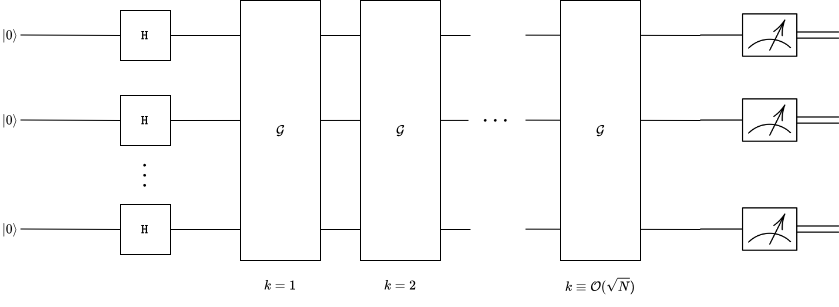
\includegraphics[width=1.0\linewidth]{body/ch2/figs/grovers-quantum-circuit}
	\caption[Generalised Quantum Circuit for Applying Grover's Search Algorithm with $k$ Iteratives.]{The quantum search algorithm applies $\mathcal{O}(\sqrt{N})$ Grover's iteratives to find the solution $x$ to an arbitrary function $f(x) \in \{0, 1\}^n$.}
	\label{fig:grover-quantum-circuit}
\end{figure}

Applications of the Hadamard and oracle $\omega$ gates can be represented on a Bloch sphere as a rotation of the two-dimensional space spanned by the starting vector and the state consisting of a superposition of the $\mu$ solutions of the solution space. The conditional phase shift on the qubits is applied to every computational basis except for the state $\ket{0}$ which receives a phase shift of -1. Overall, the oracle $G$ can be written as
\begin{align}\label{eqn:grovers-iterate}
	G & = (2\ket{x}\bra{x} - I)\Omega
\end{align}
where $I$ denotes the identity operation \cite{Nielsen2010}. After applying the last iteration $G$, the quantum search algorithm terminates with a measurement of the first $n$ qubits in the output register to obtain the solution $x$.

This paper focuses on an implementation of the quantum search algorithm using an FPGA-based quantum emulator in the computational basis. The implementation focuses on applying the procedure on a search space of size $N = 4$, corresponding to a single round of the Grover's iterative subroutine on a 3-qubit system that finds a two-bit solution $x$. Additionally, the quantum search algorithm is implemented with phase estimation in order to count the number of solutions $\mu$ to the search problem. Additionally, the design of the quantum search algorithm is restricted to structured databases which makes the implementation suitable for applications on sorted search spaces. 
 
\section{Summary \label{sec:ch2-conclusion}}
Quantum gates are unitary operations on vector states that transform the properties of qubits. This mathematical definition of quantum gates is useful in interpreting vector transformations, however, the structures represented in by the mathematics may not always be realisable. For that reason, this paper focuses on quantum gates that are realisable such as the \texttt{X}, \texttt{Z}, \texttt{H}, and \texttt{CNOT} gates. For solid state or optical quantum computers, these unitary transformations on qubits can be physical operations such as the application of a magnetic field to particles in NMR and laser pulses in ion trap implementations\cite{Rieffel2011}. Performing quantum computation can be difficult due to the probabilistic behaviour of qubits, thus, modelling systems that are costly to achieve with current technology can be useful. The theoretical framework formulated in this section forms the foundation to the concepts used to design and emulate a quantum information processing system on FPGA.

%@@@@@@@ Chapter 3 - Literature Review  @@@@@@@@@@@@@@@@@@@@@@@@@@@@@@@@@@@@@@@@@@@@@@@
\chapter{\label{ch:lit_review} Literature Review}

Integrating quantum computers to current classical systems has proven to be a difficult endeavour because of the differences between classical bits and qubits. Properties of qubits such as superposition and entanglement also make it difficult to construct heterogeneous computing systems consisting of quantum processing units (QPUs), classical central processing units (CPUs), and graphical processing units (GPUs). This chapter presents a review of existing literature on modelling quantum computer architecture on a classical machine. 

The review focuses on previous implementations and simulations of interfaces between quantum and classical computers in a heterogeneous computing system - in alignment with the scope of this paper. Furthermore, guidelines for conducting accurate FPGA-based quantum computer emulations are discussed with respect to quantum algorithm implementation and communicating the output from a quantum computer as bits to a classical computer. From this context, previous literature is use to expand the knowledge of quantum computing through an investigation of bit encoding methodologies, quantum algorithm and quantum circuit implementations in engineering applications, qubit decoding, as well as different types of quantum computer architectures that exist. In particular, the scope of the paper is limited to quantum computing algorithms that can be emulated using reconfigurable Programmable Logic Devices (PLDs) such as the FPGA.  As such, this overview of the literature accumulates quantum gate simulations that can be implemented directly at the physical level with both trapped ions and superconducting circuits.

The chapter begins by discussing applications of quantum circuit theory and implementations in quantum computing algorithms that can be performed on a FPGA-based emulated quantum computer. Then, the study investigates quantum computing architectures, communication protocols and interfaces for transmitting data between classical and quantum computers. In particular, the use of data encoding methods that have been previously implemented in engineering are discussed. The review terminates with a discourse into the overall integration and accurate simulation of heterogeneous systems containing QPUs. 

\section{Quantum Computer Realisation Criteria}


Emulating a quantum computing system on a classical device such as an FPGA requires an understanding of the fabrication of qubits, their quantum mechanical properties, and contraints on the operations that can act on them. To successfully model a quantum computer using the classical bits, it suffices to investigate the physical realisation and behaviour of qubits. In the year 2000, DiVincenzo detailed five criterion for realising a quantum computer, starting with a physical system containing a collection of qubits \cite{divincenzo2000physical}. Qubits have been realised physically as photons, nitrogen vacancies in diamonds or quantum dots in solid state systems \cite{marinescu2005promise}. Electron spin and its phase have also been controlled and manipulated to establish quantum gate transformations. In all cases, the qubits must be \textit{well-characterised}, as described in DiVincenzo's first criterion for quantum computers \cite{divincenzo2000physical}. In other words, qubits must satisfy the requirement that the general state must be expressed as a vector space with eigenvectors, $\ket{0}$ and $\ket{1}$, and normalised amplitudes, $\alpha$ and $\beta$, as shown in equation \ref{eqn:qstate}. Consequently, mappings between classical bits to qubits cannot be injective because of this fundamental difference between the two representations of units of information. However, FPGAs provide high fidelity for modelling quantum computers through logic blocks that can be connected in networks of arbitrary depth \cite{wolf2004fpga}. Since one of the objectives of this paper is to map the physical behaviour and interactions of qubits in quantum computing systems to the \gls{personality} (or program) of an FPGA that is interwoven into its logic structure.

\subsection{Well-Characterised Qubits for Realising a Quantum Computer}

According to DiVincenzo, the normalised coefficients should be accurately known. DiVincenzo extended the term "well-characterised" to mean several different things, including the presence of couplings to and interactions with other states of the qubit as implemented by Bluhm et al. who also considered the couplings of qubits to external fields by \gls{hyperfine structure}s \cite{divincenzo2000physical, bluhm2011dephasing}. DiVincenzo extends this application to two-qubit systems to emphasise that the general state of such a quantum computer can be expressed as a four-dimensional vector that can be separated into one-dimensional distinguishable sub-states of two systems \cite{divincenzo2000physical}. Using this example, DiVincenzo also cautions against the common error of considering a single-qubit system in superposition as a two-qubit system \cite{divincenzo2000physical}. Rather, such single-qubit systems that can be in two states simultaneously, must be considered as a vector space that is spanned by the states $\ket{01}$ and $\ket{10}$ \cite{divincenzo2000physical}. In modelling a quantum computer on a FPGA, the multi-level \gls{fine-grained} combinational logic elements and connectivity networks in the fabric of the device can be leveraged to emulate qubit superposition and qubit couplings in the computational basis. 

Kimble et al. implemented a method that uses a single quantum particle to describe a well-characterised qubit using measurements of the \gls{birefringence} of a single atom strongly coupled to a \gls{high-finesse} optical resonator (or cavity) ]\cite{turchette1995measurement}. Specifically, Kimble et al. demonstrated the conditional dynamics that are necessary for implementing quantum logic at the single-photon level between two frequency-distinct fields in an optical resonator by rotating the linear polarisation of a transmitted probe beam \cite{turchette1995measurement}. The well-characterised qubit was achieved from the nonlinear optical response of a Caesium (Cs) atom coupled to a cavity field with a cavity length of $\SI{56}{\micro\meter}$ \cite{turchette1995measurement}. Interactions between the photons inside the atom cavity device were investigated using the transmission of monochromatic coherent-state pump and probe beams, which were independently tunable in frequency, power and polarisation \cite{turchette1995measurement}. To quantify the strength of the photon-photon interactions, the pump and probe input fields in the quantum experiment were prepared as uncorrelated coherent states with small normalised amplitudes $|\alpha|^2$ and $|\beta|^2$ \cite{turchette1995measurement}.  Kimble et al. extended the prospects for quantum based logic by introducing the quantum phase gate (QPG) and extracting the relevant phase shifts for the truth table of the gate \cite{turchette1995measurement}. In this paper, the input to the digital system are classical bits that model the behaviour of ideal single-photon qubits. The methodology considers the initialisation of the classical bits as well-characterised qubits on a logical level, and sets constraints on the behaviour of the logic elements and connections in the FPGA to resemble the nature of the physically realised qubits. To model the preparation of uncorrelated coherent states in the emulation, qubits can be represented as a vector of size $2^n$ with complex amplitudes. Other properties of qubits - such as the no-cloning property which prohibits the duplication of a quantum state - have to be taken account as they introduce constraints on the how information should be transferred through the FPGA-emulated quantum computer.

In a 2022 study on the control of qubit transmission between quantum systems, Li, Zhang and Wu described the term "flying qubit" as quantum bits carried by travelling quantum fields \cite{li2022control}. Li et al. introduced their study by highlighting that in quantum networks, the transfer of quantum information between distant nodes can be physically realised by fabricating and capturing photons that encode these flying qubits which can range from quantum dots to microwaves from superconducting atoms \cite{li2022control}. A quantum dot can be described as a small semiconductor device with a core shell that containing free electrons \cite{marinescu2005promise}. Li et al. reference Eisaman et al.'s invited review article on single-photon sources and detectors which expands on the how photonic qubits can be generated "on-demand" using quantum dots \cite{li2022control, eisaman2011invited}.  In their 2011 article, Eisaman et al. describe the use of semiconductor quantum dots to facilitate the radiative recombination of electron-hole pair which leads to single-photon emission \cite{eisaman2011invited}. The review adds that the small size of quantum dots results in a discrete energy structure for the electrons and holes. Furthermore, the radiative lifetime of single-photon emission from optically or electrically excited quantum dots, is in the order of $\SI{1}{\nano\second}$ or less \cite{eisaman2011invited}. In the case of optically induced single-photon emission in GaAs based semiconductor quantum dots, excitation is created by photon absorption that saturates the quantum system \cite{eisaman2011invited}. Hours et al. uses a similar approach by exciting a $\SI{100}{\micro\meter}$ diameter region on GaAs/GaAlAs quantum dot with a He-Ne laser  \cite{hours2003single}. All optical measurements presented by Hours et al. were performed at $\SI{10}{\kelvin}$ in order to form a stable ground state in the GaAs/GaAsAlAs quantum well \cite{hours2003single}. Therefore, it is important to note that unlike classical bits which can be represented as high or low voltages corresponding to 0 and 1, the fabrication of qubits as single-photon also requires detectors and considerations of metrics such as the radiative lifetime. In this paper, single-photon emission from optically or electrically excited quantum dots is emulated device clocks and the radiative lifetime is represented by the pulse width.

\subsection{The Ability To Initialised Qubits to A Fiducial State}

DiVincenzo's second criterion required for the implementation of quantum information systems is the ability to initialise the state of the qubits to a simple \gls{fiducial state} \cite{divincenzo2000physical}. DiVincenzo explains that this requirement arises from the elementary computing requirement that registers should be initialised to a known value before the start of a process \cite{divincenzo2000physical}. In addition, DiVincenzo elaborates that quantum error correction requires a continuous supply of qubits in a low-entropy state such as the $\ket{0}$ basis state \cite{divincenzo2000physical}. DiVincenzo cites the need for a continuous source of 0s rather than just an initial supply, as one of the challenges in proposed implementations of quantum computers \cite{divincenzo2000physical}. 

According to DiVincenzo, for physical systems, the two main approaches for initialising quantum qubits to a standard state include cooling the system when the ground state of its Hamiltonian is the first state, or to measure and project the system into the desired state or another state on which gate operations can be performed to achieve the desired state. Prior to the publication of DiVincenzo's criteria, Imamoglu et al. propose a quantum computer in which information could be stored in the two lowest electronic states of doped GaAs quantum dots \cite{sherwin1999quantum}. Imamoglu et al. used two of the four lowest electronic energy levels to denote the states $\ket{0}$ and $\ket{1}$ for storing quantum information \cite{sherwin1999quantum}. The third energy level was used as an auxiliary state for performing conditional rotations of the state vector of the qubit \cite{sherwin1999quantum}. The state of an electron in the GaAs quantum dot was coherently manipulated by modulating the transition energies between states $\ket{0}$ and $\ket{1}$ using applied voltages to control the spacing between the energy levels \cite{sherwin1999quantum}. In fact, Imamoglu et al. describe inputting initial data as one of the core requirements for a universal quantum computer which can be achieved by arbitrary on-bit rotations effected using oscillations induced by a laser field \cite{sherwin1999quantum}.

%Another criteria for implementing a universal quantum computer that is described in literature by Imamoglu et al. relates to the ability to effect a \texttt{CNOT} gate operation as an additional requirement to initialisation of a state\cite{sherwin1999quantum}.

\subsection{Requirement for Sufficiently Long Relevant Decoherence Times}

The third criterion for implementing a quantum computer, as described DiVincenzo, states that for gate operations to be implemented physically, qubits in a quantum computer must have sufficiently long relevant decoherence times that are longer than gate operation times \cite{divincenzo2000physical}. Arguably, the primary reason for the difficulty in fabricating qubits is accounted for by the decoherence of quantum systems due to interactions of qubits with the environment. In short, decoherence times characterise the dynamics of a qubit \cite{divincenzo2000physical}. For example, in their study of electron spin decoherence in an isolated GaAs quantum dot, Khaetskii et al. found that decoherence, induced by hyperfine interactions within atomic nuclei, led to non-uniform hyperfine coupling \cite{khaetskii2002electron}. Hyperfine interactions of nuclei result from the small energy perturbations due to internally generated electric and magnetic fields. These interactions lead to \textit{decoherence}, which Marinescu describes as the randomisation of the internal state of a quantum computer due to interactions with the environment \cite{marinescu2005promise}. A key result of the study by Khaetsii et al. is that spin decay or decoherence is accompanied by the generation of quantum correlations between the electron spin and the nuclear spins which is viewed as the generation of entangled states between the qubit and its environment \cite{khaetskii2002electron}. This phenomenon is described as \textit{quantum parallelism} in decoherence. Markidis further defines \textit{quantum parallelism} - resulting from the interference of quantum state wave functions \cite{markidis2024quantum}. 

Decoherence is a principal mechanism for the emergence of classical behaviour in quantum computing that can be harnessed to perform quantum information processing \cite{divincenzo2000physical}. Conversely, if the decoherence time of a qubit is too long, then the capabilities of the quantum computer may not exceed the performance of a classical computer \cite{divincenzo2000physical}. According to DiVincenzo, decoherence may depend on the depend on the form of the initial state that can be affected by other quantum states of the qubit and in which the state amplitudes can change as well \cite{divincenzo2000physical}. Overall, the decoherence time of qubits of a system must be sufficiently long so that bits can be readout at the end of a computation \cite{sherwin1999quantum}. In their study of single-photon emission from individual GaAs/GaAlAs quantum dots, Hours et al. employ an oscillatory driving field to produce Rabi oscillations of excitons with an ultrafast radiative relaxation time in the range of 40 ps to reduce the effect of decoherence by dephasing mechanisms such as electron-phonon scattering \cite{hours2003single}. Rabi oscillations of excitons refer to the periodic alternation of electron-hole pairs between two-energy levels corresponding to a single-qubit rotation in a single quantum dot \cite{hours2003single, stievater2001rabi}. In their study of high performance emulation of quantum circuits, H\"{a}ner et al. suggest that unlike quantum simulations which directly mimic the operations that a quantum computer performs, including the effects of classical and quantum noise, a quantum emulator is only required to return the same result as a perfect and noiseless quantum computer would \cite{haner2016high}. This paper considers that although some properties of qubits such as decoherence times can be simulated, they cannot be emulated directly using classical bits.

Both Hours et al., as well as Gammon et al., excited the quantum dot through pumped laser pulses at a repetition rate in the range of $\SI{76}{\mega\hertz}$ to $\SI{82}{\mega\hertz}$, corresponding to quantum dot excitonic transitions with a time resolution determined by the pulse width, $T_1$, in the range between $\SI{6}{\pico\second}$ and $\SI{40}{\pico\second}$ \cite{hours2003single, stievater2001rabi}. In general, the $T_1$ \textit{decoherence time} characterises the duration of the transition of a qubit from an eigenstate with a higher discrete energy, such as the state $\ket{1}$, to an eigenstate in a lower energy level, such as the $\ket{0}$ basis state. The \textit{dephasing} time, $T_2$, corresponds to the time in which a qubit that is in superposition of states gradually loses phase. Gammon et al. showed that dephasing can be limited by energy relaxation at $\SI{4}{\kelvin}$ to achieve a dephasing times of $T_2 = 2T_1$ \cite{hours2003single}. For electrons in GaAs quantum dots, Bluhm et al. found that coherence times of about $\SI{1}{\micro\second}$ can revealed using spin-echo measurements at magnetic fields below $\SI{100}{\milli\tesla}$ \cite{bluhm2011dephasing}. Bluhm et al. use a spin qubit consisting of two isolated electrons confined in a double quantum dot that was created by applying negative voltages to metallic gates that locally deplete an electron gas at $\SI{90}{\nano\meter}$ below the GaAs wafer surface \cite{bluhm2011dephasing}. Bluhm et al. induced hyperfine interactions in a GaAs quantum dot by subjecting the two electrons to an effective magnetic field produced by nuclear spins \cite{bluhm2011dephasing}. The resulting Hilbert space of the logical qubit was spanned by the spin-up and spin-down combined states that can be equivalently represented as the basis states $\ket{10}$ and $\ket{01}$ \cite{bluhm2011dephasing}. In a programmable all-optical scheme for different one-qubit system, Goswami, Mandal and Mukhopadhyay implemented qubits using phase and intensity encoding of light with the help of the electro-optic modulators supported by MATLAB simulations \cite{mandal2023implementation}.

\subsection{Physical Preparation of Entangled Qubit Pairs}

Bluhm et al. initialised the ground state of the quantum system as a spin singlet with both electrons located in the neighbourhood of a single dot \cite{bluhm2011dephasing}. The electrons were successfully separated onto two quantum dots by sweeping the difference between the electrostatic potentials in the two dots to negative values, thereby preparing the Bell state $\ket{s}$, given by
\begin{align}\label{eqn:s-}
	\ket{s_-}	& = \frac{1}{\sqrt{2}}\ket{10} - \frac{1}{\sqrt{2}}\ket{01}
\end{align}
Additionally, Bluhm et al. found that very large detunings of the electrostatic potential difference between the electrons as well as the difference between the $\hat{z}$-components of the hyperfine fields in the two dots leads to energy splitting between the basis states and causes precession between the singlet state $\ket{s_-}$ and the triplet state $\ket{s_+}$, given by
\begin{align}\label{eqn:s+}
	\ket{s_+} & = \frac{1}{\sqrt{2}}\ket{10} + \frac{1}{\sqrt{2}}\ket{01}
\end{align}
The fluctuations induced by this splitting of electrons on the double quantum dots lead to dephasing of the qubit which drives coherent oscillations between the basis states \cite{bluhm2011dephasing}. Using this technique, Bluhm et al. achieved dephasing times $T_2$ exceeding $\SI{200}{\micro\second}$, which is sufficiently long to satisfy DiVincenzo's criterion regarding decoherence times - allowing a possible $10^5-10^6$ operations to be carried out on one qubit while maintaining the state of another \cite{bluhm2011dephasing, divincenzo2000physical}. Furthermore, Bluhm et al. accomplished readout of the final qubit state by using positive detuning of the electrostatic potential which led to two-spin states with different charge densities \cite{bluhm2011dephasing}. The effects of positive detuning were detected using conductance of proximal quantum point contact which depends on the local electrostatic environment \cite{sundfors1969exchange}. The average conductance, $G_{QPC}$, over many identical pulse cycles, was found to reflect the probability of finding the qubit in the singlet state at the end of each cycle \cite{bluhm2011dephasing}. 

In a similar study Imamoglu et al. proposed a tunable antenna-coupled intersubband terahertz (TACIT) quantum-well-based detector that can be integrated into a single-mode cavity that can read out qubits at roughly $\SI{300}{\mega\hertz}$ \cite{sherwin1999quantum}. In all cases, the number of events at a time interval of $\tau$ must be strictly zero \cite{hours2003single}. This implies that quantum computing systems are causal and that if a single photon is emitted and introduced to the quantum dot, it cannot activate both the start and stop channels of a microscope simultaneously \cite{hours2003single}. Hours et al. state that this is an inherent feature of photons arriving one by one \cite{hours2003single}. Hours et al. controlled the trigger of the time interval counter by permitting only photons belonging to the quantum dot emission line at $\SI{746}{\nano\meter}$ using a monochromator with a resolution of $\SI{0.5}{\nano\meter}$ \cite{hours2003single}. The excitation conditions in the experimental setup were such that the quantum dot emissions were linear and well below saturation \cite{hours2003single}. 

Using a histogram of the number of events counted as a function of the time interval between the arrivals of two successive photons, Hours et al. successfully illustrated that the emission of a start photon during excitation by a particular laser pulse corresponded to peaks at nonzero time intervals $\tau = nT$, where $n$ is the number of excitation cycles and $T = \SI{12.2}{\nano\second}$ is the laser repetition period \cite{hours2003single}. Furthermore, the peak at $\tau = 0$ corresponded to the case where both photons were obtained during the same exciting pulse \cite{hours2003single}. Hours et al. found the area of the peak at zero to have an area that was $20\%$ smaller than the other peaks and concluded that compared with coherent light pulses delivered by an attenuated laser, the probability of emitting a pair of electrons is reduced by a factor of 5 \cite{hours2003single}. Hours et al. conclude their study by noting that the photons emitted by the quantum dot have an excitonic emission line-width that was measured to be around $\SI{150}{\micro\electronvolt}$ corresponding to a dephasing time $T_2$ of $\SI{8}{\pico\second}$ and an upper bound to the exciton radiative lifetime of $T_1 < \SI{250}{\pico\second}$ \cite{hours2003single}. Spectrum broadening is accounted for by electron-electron interactions between the trapped exciton and additional electron-hole pairs, as well as due to some temperature increase due to poor heat sinking in the geometry of the microdisk \cite{hours2003single}. 

\subsection{Universal Set of Quantum Gates}

Quantum interference, or decoherence, in combination with an appropriate error correction mechanisms, allows for the retrieval of a single result that depends logically on all of the intermediate results \cite{deutsch1998quantum}. In general, existing schemes for error correction require the execution of quantum logic gates in parallel \cite{sherwin1999quantum}. The requirement for a "universal" set of quantum gates is fundamental for implementing a quantum computer, as emphasised by DiVincenzo \cite{divincenzo2000physical}. DiVincenzo highlights that if the decoherence time is $10^4$ to $10^5$ times the "clock time" of the quantum computer, then error correction can be successful \cite{divincenzo2000physical}. In this context of quantum computing, "clock time" refers to the execution time of an individual quantum gate \cite{divincenzo2000physical}. Quantum gates, which can be viewed as unitary transformations of state vectors, are crucial for the fabrication of a quantum computer since quantum algorithms are typically specified as a finite sequence of $k$ unitary transformations $U_1$, $U_2$, $U_3$, ..., $U_k$. Ideally, this sequence is applied by specifying the Hamiltonians which generate the unitary transformations, followed by calibration of the physical apparatus to perform the first Hamiltonian between time $0$ and time $t$ and subsequent Hamiltonians from time $t$ to time $2t$ and so forth \cite{divincenzo2000physical}. DiVincenzo states that in most cases, only Hamiltonians of two-qubit interactions are considered, although systems with three or more qubits can be re-expressed in with respect to sequences of single and two-qubit interactions \cite{divincenzo2000physical}. 

In order to implement the QPG transformation, Kimble et al. specified internal states by $\sigma_\pm$ polarisation and used single-photon pulses as flying qubits which propagate in two frequency-offset channels \cite{turchette1995measurement}. Ideal quantum gates cannot be implemented in real-world applications of quantum computing due to systematic and random errors in execution of the Hamiltonian transformations, therefore, error correction techniques are often required in order to produce reliable computations from unreliable quantum gate \cite{divincenzo2000physical}. DiVincenzo suggests that rate of random errors should be $10^4$ to $10^5$ per gate operation \cite{divincenzo2000physical} and that in calibrating a quantum computer, it is up to the designer to decide how much systematic error is tolerable for the system. Importantly, DiVincenzo notes that certain quantum computations, such as the quantum Fourier transform, can tolerate a very high level of systematic error over, or under rotation \cite{divincenzo2000physical}. In fulfilling the requirement for a universal set of quantum gates, one-bit gates and \texttt{CNOT} gates are usually enough to perform quantum operations \cite{divincenzo2000physical}. In 1999, Bacon et al. introduced a general scheme for performing universal, fault-tolerant quantum computations with decoherence-free subspaces by using at most two-qubit interactions \cite{bacon2000universal}. Quantum error correction uses qubit stabiliser codes to reduce the number of quantum gates \cite{chao2018quantum}. In 2018, Chao and Reichardt managed to implement a fault-tolerance scheme with minimal qubit overhead that uses Hamming codes to protect seven encoded qubits from unwanted interaction with the environment, on a device with 17 physical qubits \cite{chao2018quantum}. DiVincenzo emphasises that quantum error correction has an exceeding overhead since at least 10 or more \gls{ancilla} qubits must be added for each individual qubit of the computation \cite{divincenzo2000physical}. Additionally, unitary operations are reversible. H\"{a}ner et al. suggest that a straight-forward approach to translating a classical function to a reversible quantum circuit is to replace all the \texttt{NAND} gates by a reversible combination of single-qubit and multiple-qubit reversible gates which require an additional bit for each \texttt{NAND} to store the result \cite{haner2016high}. Then after completing the computation, the result can be copied using \texttt{CNOT} gates prior to clearing all work bits by running the entire circuit in reverse \cite{haner2016high}. However, according to H\"{a}ner et al., this transformation of a classical function to a reversible quantum circuit leads to the doubling of gates and an overhead of one qubit per \texttt{NAND} gate \cite{haner2016high}. 

\subsection{A Qubit-Specific Measurement Capability}

The final criterion expressed by DiVincenzo requires a qubit-specific measurement capability. Intuitively, this implies that the result of a computation must be read out for the implementation of a quantum computer such that given qubit with final state $\alpha\ket{0} + \beta\ket{1}$, a measurement should give an outcome of 0 with probability $|\alpha|^2$ and 1 with probability $|\beta|^2$ \cite{DeWolf2019}. Chuang and Nielsen suggest that in certain cases, measurement can be thought of a process of coupling one or more qubits to a classical system such that after some time interval, the state of the qubits is represented by the state of the classical system \cite{Nielsen2010}. Ultimately, the output from a good quantum algorithm is a superposition state which gives a useful answer with high probability when measured. To quantify the measurement capabilities of a quantum computer, the signal to noise ratio (SNR) can be used to account for measurement inefficiencies as well as inherent signal strength available from coupling a measurement apparatus to the quantum system \cite{Nielsen2010}. In superconducting quantum circuits as described by Clarke and Wilhelm, quantum computer engineers use transmon qubits which are protected against decoherence but embed all the qubits in a single resonator that is used for coupling and for joint readout \cite{clarke2008superconducting, dewes2012characterization}. Consequently, the results of a calculation cannot be obtained by running the algorithm only once as individual readout of the qubits is not possible \cite{dewes2012characterization}. H\"{a}ner et al. highlight that quantum computer emulators have an advantage over actual quantum computers when it comes to estimating the expectation values of measurements because classical emulation of such repeatedly executed measurements can easily be done in one step and the expectation value can immediately be evaluated \cite{haner2016high}. Ultimately, this removes the requirement for sampling and hence greatly reduces the overall simulation time \cite{haner2016high}. 

The discussed criteria need to be integrated into the FPGA-based emulated quantum computer through the combinational logic elements which produce an output value given an input value. The time-behaviour of the digital system also needs to correspond to the requirement for sufficiently long relevant decoherence times that are longer than gate operation times. Unlike a simulation, an emulator does not need to compile the classical function down to reversible gates and ancilla qubits \cite{haner2016high}. Instead, emulators can directly compute the desired classical function for each of its arguments and thereby, saving computational resources \cite{haner2016high}. Furthermore, results from emulating quantum programs allow to test and debug large quantum circuits at a cost that is substantially reduced compared to real quantum computers and simulations of quantum computations \cite{haner2016high}. The following section discusses the transmission of data as qubits and classical bits in a computing system that can facilitate communication of quantum information.

\section{Criteria for Quantum Communication}

In addition to having the ability to execute computations from quantum circuits, quantum information systems require communication networks to ensure that qubits can be transmitted between the different modules of the system. It follows that the criteria for implementing a quantum computer must be extended to encompass the requirements for facilitating quantum communication in order to transmit qubits between two locations while reducing \gls{crosstalk} and loss of information. In general, a quantum computing protocol can be viewed as a distributed algorithm in which the sender performs an individual computation before transmitting a message of one or more qubits to the receiver, who can also perform or computation or transmit a message back to the sender \cite{DeWolf2019}. In this paper, this execution of quantum communication protocols is managed by a microcontroller which runs a program in embedded C to initialise, transmit, as well as map qubits to classical bits. Theoretic classical computer science measures the amount of communication required to execute a function when the input is shared in a distributed network between parties as the \textit{communication complexity}. This concept of communication complexity is extended to quantum computing as the measure of the cost of quantum communication. 

\subsection{Quantum Communication Complexity}

Yao proposed one of the first quantum complexity models for structuring interactions between quantum machines \cite{yao1993quantum}. Yao defined the quantum complexity of a function $f(x,y)$ as the minimum communication cost of any interacting pair of quantum circuits for computing a function $f$, with $x \in X$ and $y \in Y$ being the respective inputs to the interacting quantum circuits \cite{yao1993quantum}. Analogous to classical communication complexities, de Wolf describes the cost of a communication protocol as the total number of qubits transmitted given an input that produces a worst-case output \cite{DeWolf2019}. Among the primary objectives of classical communication complexity models is to compute some function $f$ that maps a domain $\mathcal{D}$, which is a subset of the cross-product of the input domains $X$ and $Y$, to a binary set $\{0,1\}$, using a minimal cost of communication \cite{DeWolf2019}. 

Yao's quantum communication complexity model allocates three parts to the total state, namely, the sender's private quantum system, the communication channel, and the receiver's private quantum system \cite{DeWolf2019, yao1993quantum}. The initial state of the protocol is therefore $\ket{x}\ket{0}\ket{y}$, i.e., the sender measures the input $x$, the channel qubit is initialised to the ground state, and the receiver is allocated the output $y$ \cite{DeWolf2019}. The sender applies unitary transformations and initialises the message for transmission on the communication channel \cite{DeWolf2019}. 

Typically, the length of the message is equal to the number of channel-qubits affected by the sender's unitary operations on their system \cite{DeWolf2019}. Since the qubits are communicated through the channel, the quantum computing apparatus must have the ability to interconvert stationary and flying qubits and must also have the ability to faithfully transmit flying qubits between the sender's private space and the receiver's private space \cite{divincenzo2000physical}. DiVincenzo also notes that in some cases, for instance quantum cryptography, on the requirement for interconversion of stationary and flying qubits suffices to implement the quantum communication protocol \cite{divincenzo2000physical}. Some proposals of quantum communication protocols assume that photon states, with the flying qubit encoded either in the polarisation or in the spatial wavefunction of the photon, can be developed using the technology of light transmission through optical fibres \cite{divincenzo2000physical}. At the end of the communication proposed by Yao, the sender and the receiver make a measurement to determine the output of the protocol \cite{DeWolf2019}. 

\subsection{Physical Realisations of Quantum Communication Channels}

In 1999, Chuang and Gottesman demonstrated the viability of universal quantum computation and communication using \textit{quantum teleportation} \cite{gottesman1999demonstrating}. Quantum teleportation is a distributed scheme through which the state a qubit can be transported from one point to another by communicating with only two classical bits \cite{gottesman1999demonstrating}. In this scheme, the sender and receiver are required to share halves of a two-qubit entangled EPR state $\ket{\psi^\pm}$ prior to initialising communications \cite{gottesman1999demonstrating}. A single-qubit state $\ket{\psi_0}$ is prepared by the sender along with the EPR pair \cite{gottesman1999demonstrating}. 

The sender performs Bell measurements on both $\ket{\psi_0}$ and one qubit of the EPR pair. Chuang and Gottesman highlighted that given any input state $\ket{\psi_0}$ as illustrated in the quantum circuit for teleportion in figure \ref{fig:chuang-teleportation}, the classical output from the Bell state measurement is a uniformly distributed random two-bit classical result, $ab$ \cite{gottesman1999demonstrating}. Additionally, measurements leave the third qubit belonging to the receiver in a transformed state $R_{ab}$ of the initial qubit $\ket{\psi_0}$, where $R_{ab}$ is either the identity corresponding to no transformation when $ab = 00$, or a single-qubit Pauli transformation such as the $X$ or $Z$-gate transformations \cite{gottesman1999demonstrating}. To complete the quantum teleportation, the sender transmits the two classical bits $ab$ to the receiver who can use them to apply error correction using the inverse unity operation of $R_{ab}$, thereby reconstructing an output $\ket{\psi_0}$ which is identical to the original input \cite{gottesman1999demonstrating}. Evidently, quantum teleportation introduces a larger overhead in communication complexity compared to the protocol proposed by Yao which only requires two qubits and a flying qubit on the communication channel \cite{DeWolf2019}. 

\begin{figure}[!ht]
	\centering
	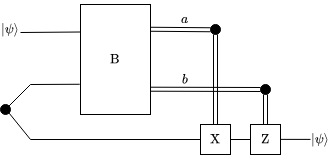
\includegraphics[width=0.75\linewidth]{body/ch3/figs/chuang-teleportation}
	\caption[Quantum Circuit for Quantum Teleportation by Chuang and Gottesman.]{This quantum circuit demonstrates how quantum teleportation uses measurements to transfer states from on place to another \cite{gottesman1999demonstrating}. The symbol with the black dot and diverging wire to the left of the circuit represents an EPR state and the box $B$ represents a Bell measurement of the input states. Double lines represent classical outputs.}
	\label{fig:chuang-teleportation}
\end{figure}

In order for sender A to convey $n$ bits of information to the receiver B, \textit{Holevo's theorem} states that, where quantum entanglement is available and qubit communication in either direction is permitted, A must send B at least at $\lceil n/2 \rceil$ qubits \cite{cleve1998quantum, holevo1998quantum}. Holevo's theorem holds regardless of the prior entanglement and communication from B to A \cite{cleve1998quantum}. A consequence of Holevo's theorem is that a low-dimensional quantum computer, with a small number, cannot contain too much accessible information \cite{DeWolf2019}. Another consequence of Holevo's theorem that was derived by Cleve et al. and elaborated on by de Wolf can be demonstrated using the case where sender A wants to communicate a string $x$ to receiver B \cite{cleve1998quantum, DeWolf2019}. If A sends $m$ qubits to B, and both parties did not share some prior entangled state, then B receives at most $m$ bits of information about $x$ \cite{cleve1998quantum, DeWolf2019}. Conversely, if A sends B $m$ qubits, and they share some prior entangled state, then B receives at most $2m$ bits of information about string $x$ \cite{cleve1998quantum, DeWolf2019}. Furthermore, if A sends B $m$ classical bits, and they shared some prior entangled state, then B receives at most $m$ bits of information about $x$ \cite{cleve1998quantum, DeWolf2019}. Thus, despite having $2^m$ complex amplitudes, an $m$-qubit quantum computer is no better at potentially storing or transmitting information than a classical computer with $m$-bit wide registers and communication channel bandwidths \cite{DeWolf2019}. However, prior entanglement can improve the performance of quantum communication when superdense coding properties are considered \cite{DeWolf2019}. Additionally, by sharing prior entangled states, the qubit on the sender's side is destroyed, which prohibts unknown qubits from being copied in a quantum computer \cite{DeWolf2019}.

\subsection{Communication in Quantum Key Distribution Networks}

According to an artical by Wootters in 1982, cloning qubits is prohibited by linearity of quantum mechanics \cite{wootters1982single}. The no-cloning property of qubits makes quantum computers suitable for cryptography and secure communication. In particular, the principles of quantum communication explored here are useful for Quantum Key Distribution (QKD) networks. The goal of QKD is to allow point-to-point communication between two remote parties linked by a quantum channel and an authenticated classical channel to share a common random binary string known as a \textit{key} \cite{salvail2010security}.  According to Salvail et al., a QKD network is an infrastructure that is capable of performing long-distance and high-rate secret key agreements \cite{salvail2010security}. QKD networks perform key establishment methods which are based on protocols, including locally executed algorithmic steps and public communication \cite{salvail2010security}. 

A QKD network developed by the Secure Communication based on Quantum Cryptography (SECOQC) project in consists of node modules which enable authentic classical communication required for key distillation, manages the generated key material, determines a communication path between any destinations in the network, and establishes secure transport of key material between destinations \cite{peev2009secoqc}. The network topology of the SECOQC QKD network consists of a Coherent One-Way (COW) time coding system that uses a novel distributed phase reference COW protocol to enable communication for up to $\SI{85}{\kilo\meter}$ \cite{peev2009secoqc}. At the start of the protocol, the sender prepares pulses of weak coherent states using a Continuous-Wave (CW) laser with a wavelength of $\SI{1550}{\nano\meter}$ and an intensity modulator \cite{peev2009secoqc}. The logical bits 0 and 1 are encoded in two-pulse sequences, which can be written as a product of coherent states $\ket{\sqrt{\mu}}$ and $\ket{\sqrt{0}}$ such that the $k$-th logical qubit is given by
\begin{align}\label{eqn:secoqc-kth-bit}
	\ket{0_k}	& = \ket{\sqrt{\mu}}_{2k-1} \ket{\sqrt{0}}_{2k}\nonumber\\
	\ket{1_k}	& = \ket{\sqrt{0}}_{2k-1} \ket{\sqrt{\mu}}_{2k}
\end{align} 
These encoded states are not orthogonal, however, a conclusive ToA measurement can provide the optimal unambiguous determination of the bit value \cite{gisin2004towards}.

Pulses propagate to receiver B through a quantum channel characterised by a transmission channel $t$ and are separated at a beamsplitter with a transmission coefficient $t_B \leq 1$ such that only $10\%$ of the pulses are reflected into B's \gls{interferometer} to check for quantum state coherence \cite{peev2009secoqc}. Due to the large coherence times of the CW laser, there is a well-defined phase between any two non-empty pulses across the bit separation and within decoy sequences. The receiver measures the time-of-arrival (ToA) of these pulses to provide an unambiguous determination of bit values and establish the raw key. The COW QKD system can detect an attack by an eavesdropper by using InGaAs single-photon laser diodes operating with an intensity modulator to produce signal and decoy pulses that can be measured behind an \gls{interferometer} as illustrated in figure \ref{fig:cow-protocol} \cite{peev2009secoqc}. To ensure security, the wavelength of A's laser is adjusted in a way that only one of two monitoring detectors at the receiver is triggered \cite{peev2009secoqc}. 
\begin{figure}[!ht]
	\centering
	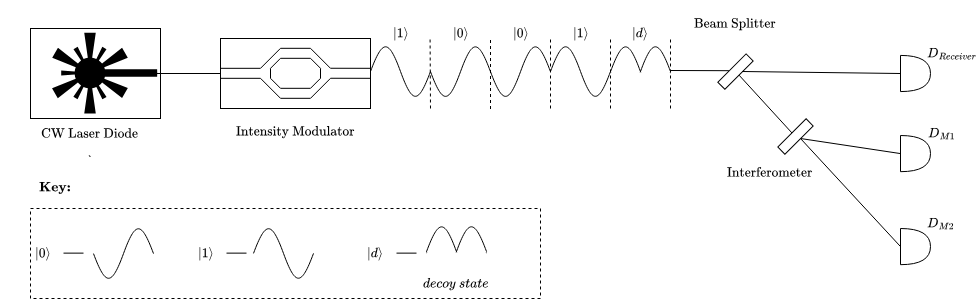
\includegraphics[width=1.0\linewidth]{body/ch3/figs/cow-protocol}
	\caption[Coherent One-Way (COW) Quantum Key Distribution System by GAP University of Geneva.]{The sender's CW laser and intensity modulator are illustrated on the left and the receiver's InGaAs detectors are illustrated to the right. The COW QKD system's CW laser has large coherence length to prevent phase-shift and photon number splitting attacks by producing a well-defined phase between two non-empty pulses across a bit sequence and within a decoy sequence \cite{peev2009secoqc}. Pulses propagate through a quantum channel to InGaAs detectors at the receiver. The main receiver detector $D_{Receiver}$ checks quantum coherence, while detectors $D_{M1}$ and $D_{M2}$ ensure security by revealing any action by an eavesdropper.}
	\label{fig:cow-protocol}
\end{figure}
The SECOQC QKD network also includes a one-way weak pulse system implemented by Toshiba Research Europe Ltd (TREL) that transmits optical pulses with a wavelength of $\SI{1.55}{\micro\meter}$ along a quantum channel at a repetition rate of about $\SI{7}{\mega\hertz}$ \cite{peev2009secoqc}. TREL used strong clock pulses with a duration of $\SI{5}{\nano\second}$ each and that do not overlap with the signal pulses to establish synchronisation between the different parts of the system \cite{peev2009secoqc}. An intense modulator is used to produce decoy sequences that are strongly attenuated to the single-photon level and the strong clock pulse is multiplexed with the decoy pulses to provide synchronisation \cite{peev2009secoqc}. The receiver uses two single-photon InGaAs avalanche photodiodes (APDs) as detectors that are adjusted to avoid fake-state attacks and time-shift attacks \cite{peev2009secoqc}. The receiver cannot use a modulator or optical attenuator to secure the system because the attenuator would absord a large percentage of all the single photons from the sender \cite{lydersen2011secure}. Fake-state attacks exploit the classical photodiode mode of the APD by triggering the detector in the presence of bright pulses \cite{lydersen2011secure}. 

\subsection{Methods for Preventing Fake-Attacks and Time-Shift Attacks}

Lydersen et al. proposed background illumination to keep the APDs in the classical photodiode mode so that the detectors only respond to bright optical trigger pulses and not single-photons \cite{lydersen2011secure}. Fake-attacks can also be prevented by using gated APDs whose single-photon sensitivity is based on measurements of time-of-arrival. Time-shift attacks are based on detector efficiency mismatch (DEM) in the time-domain \cite{lydersen2011secure}. For example, if the receiver B's apparatus contains two single-photon detectors (SPDs) for incoming photons - one for each bit value - the detection windows and hence the efficiency curves of the two detectors would be slightly shifted \cite{lydersen2011secure}. Lydersen et al. performed an experiment where an eavesdropper E was able to capture partial information about the key in $4\%$ of all time-shift attacks attempts \cite{lydersen2011secure}. For a short SECOQC QKD fibre link of $\SI{1}{\kilo\meter}$, TREL were able to achieve a high secure bit rate of $\SI{27}{\kilo\bit\per\second}$ for $24$ hours \cite{peev2009secoqc}. 

A QKD system that exploits entanglement was developed by an Austrian-Swedish consortium for generating secure keys as part of the SECOQC QKD network \cite{peev2009secoqc}. The schematic of the system in figure \ref{fig:ent-qkd} shows the optical and electronic connections between the different components. When the system is initialised, the entanglement source at sender A's location produces polarisation-entangled photon EPR pairs at $\SI{810}{\nano\meter}$ and $\SI{1550}{\nano\meter}$ \cite{peev2009secoqc}. The $\SI{810}{\nano\meter}$ photon is detected using four silicon-based APDs with four phase-encoded polarisation basis states $\{\ket{-\pi/4}$,$\ket{0}$,$\ket{\pi/2}$,$\ket{\pi/4}\}$ while the $\SI{1550}{\nano\meter}$ photon is transmitted to receiver B using single-mode fibres (SMF) \cite{peev2009secoqc}. The $\SI{1550}{\nano\meter}$ photon of the EPR pair travels through the quantum channel with low transmission losses and is registered by the receiver using passive polarisation analysers with four InGaAs avalanche photodiodes \cite{peev2009secoqc}. The receiver uses FPGAs to analyse the synchronised pulse arriving at four InGaAs-APDs with the same phase-encoded polarisation states \cite{peev2009secoqc}. 
\begin{figure}[!ht]
	\centering
	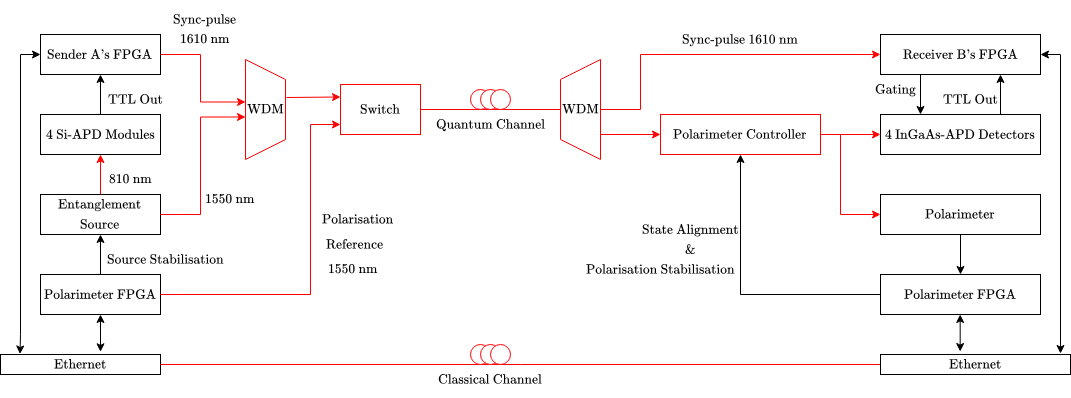
\includegraphics[width=1.0\linewidth]{body/ch3/figs/ent-qkd}
	\caption[Schematic of the Ent Quantum Key Distribution System in the SECOQC Network by the Austrian Institute of Technology at the University of Vienna.]{The Ent QKD system generates a secure key using Bell state measurements of entangled qubits at the location of the transmitter and the receiver. The source creates polarisation entangled photon pairs at highly non-degenerate wavelengths which are locally analysed in four polarisation states. FPGAs are used to process all detection events and logged onto computers \cite{peev2009secoqc}.}
	\label{fig:ent-qkd}
\end{figure}
More FPGAs are used to control the source stabilisation module at the sender's location as well as for implementing \gls{polarimeter} modules at both ends of the point-to-point communication \cite{peev2009secoqc}. The source stabilisation modules use automatically adjusted \gls{piezo-actuated} fibre couplers to achieve maximum photon detection rates to ensure that the photon flux emitted from the crystal is efficiently coupled to the SMFs leading to the detectors at A and B \cite{peev2009secoqc}. Polarimeter modules control the polarisation to ensure that the QKD system produces a reliable and stabilised distribution of phase-encoded qubits in the optical fibre-based quantum channels \cite{peev2009secoqc}. Similar to the COW QKD system, the Ent QKD system synchronises the trigger signals used to gate the receiver's InGaAs-APDs must be synchronised to initialise the detection window when a single photon is expected \cite{peev2009secoqc}. 

\section{Bit Mapping and Qubit Mapping for Quantum Computing Hardware Platforms}

When referring to APDs, Lydersen et al. use the term 'gated' to refer to the ability of an APD detector to be single-photon sensitive only when a photon is expected to arrive, i.e. in the detection window \cite{lydersen2011secure}. Lydersen et al. employed the concept of gating detectors to present a method for securing Bob's receiver called \textit{bit-mapped gating} which protects the system against pulses from regions that are outside the central neighbourhood of the detector gate in the implemented protocol \cite{lydersen2011secure}. Bit-mapped gating is implemented in software to determine how the signals from detectors $a$ and $b$ are mapped into the logical bits $0$ and $1$ \cite{lydersen2011secure}. Optical bit mapping defines the relationship between the detectors, $a$ and $b$, and the quantum states with qubit values $\ket{0}$ and $\ket{1}$ in the $Z$ basis \cite{lydersen2011secure}. Software and optical bit mapping need to coincide in order to ensure that the bit value sent by A matches the value received by B. 

\subsection{Optical Bit Mapping}

Bit-mapped gating is implemented between the detector gates and begins with receiver B randomly assigning detectors $a$ and $b$ values of 0 and 1 \cite{lydersen2011secure}. Following the selection of the software bit mapping, the basis is selected randomly between the $X$ basis which corresponds to the $\pi/2 \si{\radian}$ phase shift and the $Z$ basis corresponding to the $0 \si{\radian}$ phase shift along with random optical bit mapping \cite{lydersen2011secure}. Figure \ref{fig:optical-bit-mapping} shows an example of a timing diagram used by Lydersen et al. to represent possible optical bit mapping schemes \cite{lydersen2011secure}.
\begin{figure}[!ht]
	\centering
	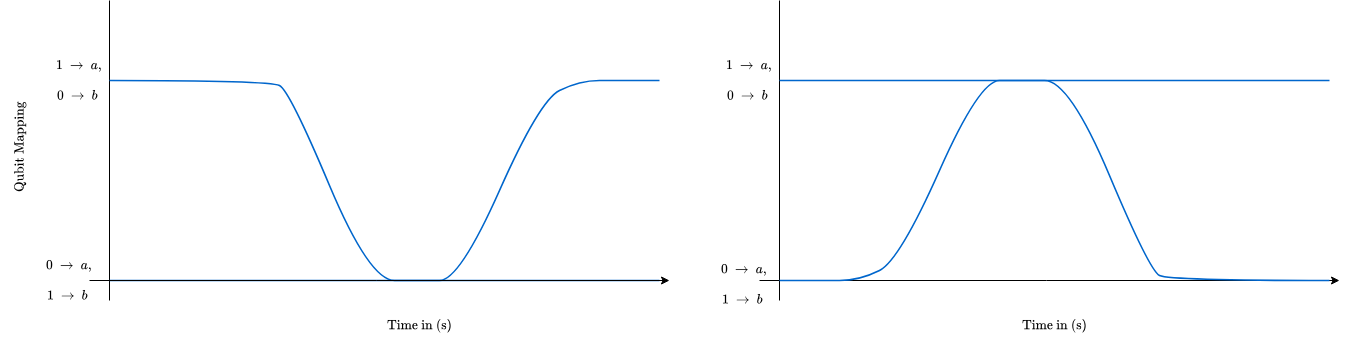
\includegraphics[width=1.0\linewidth]{body/ch3/figs/optical-bit-mapping}
	\caption[Timing Diagram for Possible Optical Bit Mapping Scheme by Lydersen et al.]{Showing possible optical bit mappings corresponding to $0$ and $\pi$ phase shift in one basis, and $\pi/2$ and $3\pi/2$ in the opposite basis \cite{lydersen2011secure}.}
	\label{fig:optical-bit-mapping}
\end{figure}
Lydersen et al. noted that in a phase-encoded system, the two levels would correspond to a phase of $0$ and $\pi \si{\radian}$ \cite{lydersen2011secure}. Detector gates facilitate software and optical bit mapping correspondence \cite{lydersen2011secure}. A bit-mapped gate refers to the period of matching optical and software bit mapping \cite{lydersen2011secure}. The aim of bit mapping is to ensure that all states received and detected outside the bit-mapping gate cause random detection results by applying randomised selection in optical and software bit mapping, and thereby improving the security of a QKD system \cite{lydersen2011secure}. Detections in the middle of the gate produce a quantum bit error rate (QBER) of $0\%$, whereas detections outside the centre produce a QBER of $50\%$ \cite{lydersen2011secure}. Lydersen et al. also showed that multiple photons detected individually in a single optical mode, corresponding to the ToA $t$, increase the minimum QBER \cite{lydersen2011secure}. This can be accounted for by the fact that when each photon hits a separate set of detectors and the detection results are merged to give the detection results of threshold detectors \cite{lydersen2011secure}. 

\subsection{Differentiating Between Physical Qubits and Logical Qubits}

In the application of quantum computers for approximate combinatorial optimisation, Farhi et al. differentiated between a \textit{physical qubit} from a \textit{logical qubit} to employ a sequence of parametrised unitary operations that sit on the qubit layout to produce quantum states based on the parameters  \cite{farhi2017quantum}. In essence, a logical qubit is a physical or abstract qubit that forms part of a quantum algorithm or quantum circuit and is mapped onto a physical qubit, which is a quantum particle or device whose behaviour can be described by the $\ket{0}$ and $\ket{1}$ basis state \cite{zhang2021time}. Alternatively, the quantum computer can produce quantum states whose discretised energy is near the ground state energy of a given quantum-well with a given Hamiltonian $H$ \cite{farhi2017quantum}. Ultimately, both implementations of quantum computers satisfy DiVincenzo's criterion for initialising a qubit to a ground state $\ket{0}$ \cite{farhi2017quantum, divincenzo2000physical}. Furthermore, the quantum computers both have a sequence of universal unitary transformations that act on the initial state to produce a desired quantum state $\ket{\mathbf{\nu}}$ that depends on the eigenvalues and linear coefficients of the unitary operations \cite{farhi2017quantum}. Given $L$ unitary operations, corresponding to $L$ quantum gate operations, Farhi et al. write the desired state as, 
\begin{align}\label{eqn:desired-state-from-initial}
	\ket{\underline{\nu}} & = U_L(\nu_L)\cdots U_1(\nu_1)\ket{0}
\end{align} 
where $\mathbf{\nu}$ denotes the collection $\nu_1,...,\nu_L$ of parameters and each quantum gate operation $U_i$ depends on this set of parameters \cite{farhi2017quantum}. The aim of the combinatorial optimisation quantum algorithm is to choose the parameters $\mathbf{\nu}$ such that the expected value of the objective function $C$ is maximised or such that that the expected value of the Hamiltonian $H$ is small \cite{farhi2017quantum}. An $n$ qubit quantum computer produces states as shown in \ref{eqn:desired-state-from-initial} and a classical optimisation routine that takes as input, a sequence of parameters $\mathbf{\nu}$ associated with maximal expectation values and outputs a new value of the parameters \cite{farhi2017quantum}. The pseudocode of the algorithm takes a classical objective function $C$ on $n$ strings that can efficiently be evaluated on any input string $z$ as the input \cite{farhi2017quantum}. 

In the procedure, a repetition number $R$ is selected along with a stopping criterion which may depend on the quality of the objective function value or the number of clock cycles of the quantum computers. Then, the quantum computer is started by initialising the ground state and one of the $n!$ ways of assigning the $n$ bits associated with the objective function to the physical qubits \cite{farhi2017quantum}. After selecting the initial set of parameter in the collection $\mathbf{\nu}$, the algorithm runs until for $R$ times or until the stopping criterion is satisfied. In loop, a measurement is performed in the computational basis which produces a string $z$ for evaluating the objective function $C$ \cite{farhi2017quantum}. Finally, the algorithm outputs the string $z$ with the highest value of $C(z)$. Farhi points out that although it suffices to only consider objective functions that can be written as a sum of individual terms involving two classical bits, the connectivity of the objective function may have nothing to do with the pairwise connectivity of physical qubits in the hardware \cite{farhi2017quantum}. 

Qubit pairs that can be acted on by two-qubit gates depend on the hardware architecture \cite{farhi2017quantum}. The qubits on the hardware can also be labelled as $\ket{1}_{10}$,...,$\ket{n}_{10}$, corresponding to the total number of qubits of the quantum computer. In the space-time volume of a quantum computation, Farhi et al. arrange $n$ qubits in a $\sqrt{n}\times \sqrt{n}$ grid array which is initialised by preparing the quantum state of each qubit \cite{farhi2017quantum}. Each qubit is coupled to 4 other qubits except at the borders of the grid. Layers of single-qubit gates and two-qubit gates act on the qubits with operations that are restricted by the hardware architecture \cite{farhi2017quantum}. 

\subsection{Modelling Quantum Computers with Physical and Logical Qubits}

In a similar study of the qubit mapping problem, Li, Ding and Xie suggest that based on a given quantum circuit and the coupling information of the device, a quantum computing solution requires an initial logical-to-physical qubit mapping and an intermediate mapping transition which is able to remap two logical qubits in a two-qubit gate to two coupled physical qubits \cite{li2019tackling}. Li et al. developed a flexible \texttt{swap} gate-based heuristic algorithm, called SABRE, for finding the optimal solution to the qubit mapping problem which is applicable to Noisy Intermediate-Scale Quantum (NISQ) devices with arbitrary connections between qubits \cite{li2019tackling}. Li et al. noted that for NISQ devices, such as the IBM Q20 quantum processor, the assumption that two-qubit gates can be applied to arbitrary two logical qubits in a quantum algorithm does not hold \cite{li2019tackling}. This is because when running a quantum program, logical qubits need to be mapped to the physical qubits, analogous to register allocation in classical computing but for physical qubits NISQ devices, a qubit can only couple with its nearest neighbour so that for a specific mapping, two-qubit pairs can only be applied to limited logical qubit pairs \cite{li2019tackling}. Therefore, a quantum circuit cannot be directly implemented on NISQ devices \cite{li2019tackling}. To resolve this limitation of NISQ devices, qubit mappings and circuit transformations are required to make the circuit compatible during compilation \cite{li2019tackling}. 
   
According to the \textit{Gottesman-Knill theorem}, a computation that involves state operations in the computational basis, Hadamard gates, phase gates, controlled-\texttt{NOT} gates, single-qubit Pauli gates, and measurements of observables in the Pauli group, may be simulated efficiently on a classical computer \cite{Nielsen2010}. Li et al. exploited this fact to develop the SABRE algorithm with the observation that effective mapping transition needs to start from the qubits in the two-qubit \texttt{CNOT} gates that need to executed on an IBM 20-qubit chip model \cite{li2019tackling}. Before extending the application of the algorithm to 20 qubits, Li et al. use a small-sized 4-qubit device model as the hardware platform as an example for demonstrating initial logical-to-physical qubit mappings. In the 4-qubit device model, two-qubit gate operations are only allowed on the physical qubit pairs $\{Q_1, Q_2\}$, $\{Q_2, Q_4\}$, $\{Q_3, Q_4\}$ and $\{Q_1, Q_3\}$ \cite{li2019tackling}. Assuming that the initial logical-to-physical qubits mapping is $\{q_1 \rightarrow Q_1, q_2 \rightarrow Q_2, ...\}$, the execution of a quantum circuit with six \texttt{CNOT} gates to the device requires only four out of the six gates because the fourth and the sixth gates cannot be executed since the corresponding qubits are not coupled \cite{li2019tackling}. 

The SABRE algorithm approximates a perfect initial mapping to satisfy all two-qubit gate dependencies by employing \texttt{swap} gates that change the qubit mapping by exchanging states between two qubits to make all \texttt{CNOT} gates executable without changing the overall functionality of the circuit \cite{li2019tackling}.  The use of \texttt{swap} gates increases the number of operations in the circuit which carry imperfections that introduce noise and hence, the overall error rate \cite{li2019tackling}. Additionally, introducing \texttt{swap} gates to the qubit mapping increases the circuit depth, which leads to an increase in the total execution time and error accumulation from qubit decoherence \cite{li2019tackling}. Three \texttt{swap} gates are introduced in the initial qubit mapping, increasing the total number of gates in the circuit from $6$ to $9$ gates and increasing the circuit depth from $5$ to $8$ \cite{li2019tackling}. Figure \ref{fig:li-qubit-mappings} illustrates the original quantum circuit with 6 \texttt{CNOT} gates alongside the updated hardware-compliant quantum circuit with 3 additional \texttt{swap} \cite{li2019tackling}. 

\begin{figure}[!ht]
	\centering
	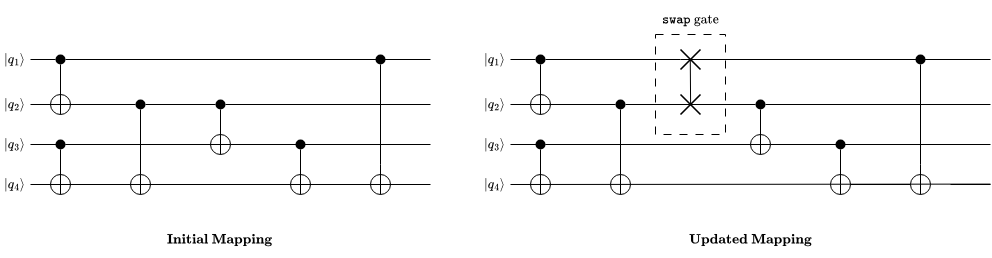
\includegraphics[width=1.0\linewidth]{body/ch3/figs/li-qubit-mappings}
	\caption[Hardware-Compliant Quantum Circuit for a 4-qubit Device by Li et al.]{In their article, Li et al. proposed the used of \texttt{swap} gates to change the qubit mappings to allow all the \texttt{CNOT} gates to circumvent the logical-to-physical qubit mapping problem where corresponding qubit pairs are not connected. \cite{li2019tackling}.}
	\label{fig:li-qubit-mappings}
\end{figure}

Li et al. implemented the SABRE algorithm in the Python coding language without any parallelisation or acceleration \cite{li2019tackling}. The heuristic search experiments were executed on a server with Intel Xeon E5-2680 CPUs containing 48 logical cores each and $\SI{48}{\giga\byte}$ of memory. Compared to other algorithms such as Zulehner et al.'s Best Known Algorithm (BKA) which required $\SI{40}{\giga\byte}$ memory and $\SI{474.81}{\second}$ execution time, the SABRE algorithm was observed to be more efficiency, requiring about $\SI{200}{\mega\byte}$ memory and $\SI{0.08}{\second}$ runtime \cite{li2019tackling, zulehner2018efficient}. Zulehner et al.'s BKA algorithm differs from the SABRE algorithm in that it searches all possible combinations of \texttt{swap} gates that can be applied concurrently to minimize the output circuit depth and the number of additional \texttt{swap} gates at the same time which requires $\mathcal{O}$, whereas the SABRE algorithm uses a heuristic cost function to help find the \texttt{swap} that can reduce the sum of distances between each qubit pair in the front layer \cite{zulehner2018efficient, li2019tackling}.  

The metrics for evaluating the qubit mapping efficiency discussed above, including the QBER, total number of quantum gates used, quantum circuit depth, memory usage and execution time form an essential part for benchmarking the FPGA-based emulated quantum computing system. The following section discusses existing frameworks for emulating the different properties of quantum computers on FPGA-based hardware accelerators.

\section{Representations of Qubits in FPGA-Based Quantum Computer Emulations \label{sec:lit-qubit-rep}}

While studying the emulation of quantum systems on FPGA, Minoru Fujishima noted that realisation of a quantum computer with large-scale qubits is difficult in both physical quantum mechanical processes and software simulation \cite{fujishima2003fpga}. The quantum state of a qubit is directly related to the complex and real parts of the normalised amplitude coefficients in the linear combination of the state vectors $\ket{0}$ and $\ket{1}$ which collapse to a single value depending on the magnitude of the probabilistic complex coefficient. As the number of qubits $n$ in the system is increased, the computational requirements for storing and manipulating the $2^n \times 2^n$ dense matrices involved in quantum algorithms also increased. To efficiently model qubits in the FPGA-based emulation, careful consideration needs to be taken on the design and implementation of qubits and a concise methodology needs to be defined for the transformations that can be performed on them. Typically, emulations of quantum computers on FPGA focus on optimising the storage and manipulation of the complex coefficients as fixed-point or floating-point numbers \cite{Aminian2008, Hlukhov2021, Khalid2004, Khalil2015}.  

\subsection{Assigning Probabilities to Input-and-Output Tables}

The focus of Fujishima's study was in solving \gls{NP-complete} problems in polynomial time using a quantum computer. In finding solutions to NP-complete problems with output $y = f(x)$, the aim is to find the input $x$ for the output $y$. To solve problems of this class, Fujishima used the QFT in Shor's algorithm to find the solution for periodic input-and-output pairs in polynomial time \cite{fujishima2003fpga}. When the input-and-ouput pairs of the system were not periodic, Fujishima noted that using Grover's search algorithm increased the computational time proportional to the square root of the number of input-and-output pairs \cite{fujishima2003fpga}. 

Fujishima assigned separate qubits for the input $x$ and the output $y$ such that all the output registers correspond to input registers and the same qubit cannot be used foar an output and an input \cite{fujishima2003fpga}. For example, a simple 2-qubit quantum computer with 2 input registers and 2 corresponding output quantum registers is shown in figure \ref{fig:fujishima-inout} where the input and output qubits for generating the input-and-output table are labeled $\ket{q_0q_1}$, and $\ket{q_2q_3}$, respectively \cite{fujishima2003fpga}. Separate qubits were added during the calculation according to the number of ancilla qubits required in the quantum algorithm \cite{fujishima2003fpga}. To optimise the emulation pipeline, Fujishima dealt with qubits using two different approaches, namely, a logic quantum processor (LQP) and a quantum index processor (QIP). 

\begin{figure}[!ht]
	\centering
	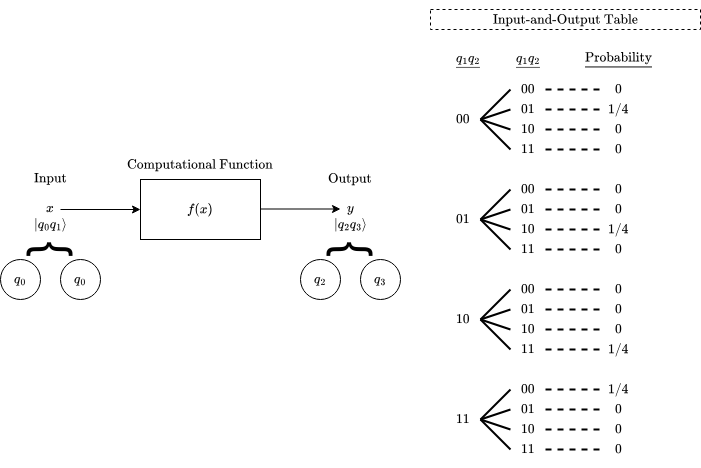
\includegraphics[width=1.0\linewidth]{body/ch3/figs/fujishima-inout}
	\caption[Input-and-Output Table by Fujishima.]{In the first stage of the FPGA-based emulation pipeline proposed by Fujishima, the input-and-output table is generated to solve an NP-complete problem with input $x$ and output $y=f(x)$ using a quantum computer. Fujishima suggests that the qubit input-and-output table shown needs to be generated in polynomial time \cite{fujishima2003fpga}.}
	\label{fig:fujishima-inout}
\end{figure}

Fujishima noted that for the quantum algorithm to be executed in polynomial time, the table of input-and-output qubit pairs should also be generated in polynomial time. This can by achieved by encoding information in the period of the outputs of the input-and-output table prior to the first step of the emulation pipeline \cite{fujishima2003fpga}. The first step of the emulation pipeline that uses a logic process distributes the probabilities equally to the quantum states corresponding to the candidate answer in the quantum search algorithm that finds the correct input-and-output pair in the table \cite{fujishima2003fpga}. Only two probabilities appear in the table, i.e. 0 and $1/m,~~m\in\mathbb{Z}^+$, before the second stage \cite{fujishima2003fpga}. 

In each case, the number $m$ corresponds to the number of entries in the input-and-output table. Thus, using the different registers for the input and output allowed Fujishima to design a LQP that expresses probabilities in binary \cite{fujishima2003fpga}. The QIP was developed to improve memory usage by observing that the output depends on the location of 1 in the quantum states used as inputs to the input-and-output table \cite{fujishima2003fpga}. Fujishima designated the term quantum index to refer to the location of 1 in the QIP. To illustrate the difference in the amount of memory used by the QIP compared to the LQP in order to process quantum states, Fujishima used the illustration in \ref{fig:fujishima-lqp-qip}, showing that the QIP is only required to store half the number of quantum states related to the candidate solution in the input-and-output table \cite{fujishima2003fpga}. 

\begin{figure}[!ht]
	\centering
	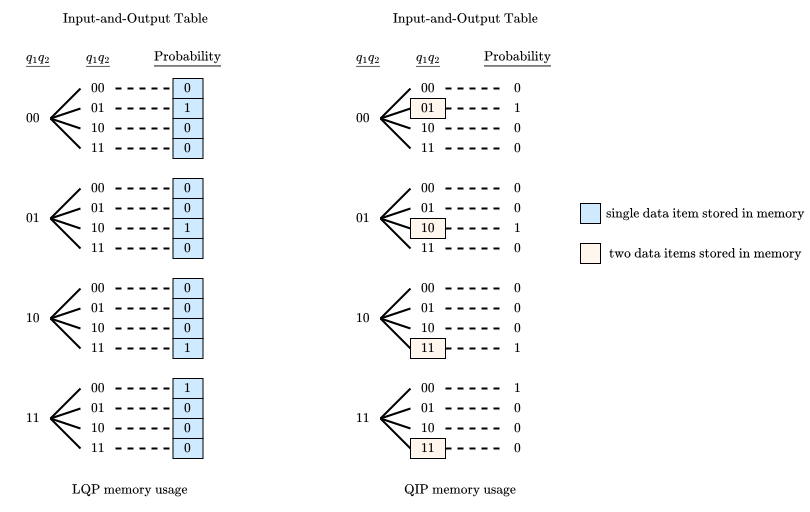
\includegraphics[width=1.0\linewidth]{body/ch3/figs/fujishima-lqp-qip}
	\caption[Memory Comparison for Logic Quantum Processor (LQP) and Quantum Index Processor (QIP).]{In comparison, the LQP uses more memory than the QIP for the same input-and-output table. An LQP implementation requires all probabilities to be stored in memory, whereas the QIP only stores the quantum index.}
	\label{fig:fujishima-lqp-qip}
\end{figure}

A FPGA with 1.5 million gates was used to implement a QIP with 2048 processing elements, corresponding to 11 qubits \cite{fujishima2003fpga}. Each processing element was driven by a clock at $\SI{80}{\mega\hertz}$ and consisted of logic unit, a memory block and a temporary register as illustrated in figure \ref{fig:fujishima-qip-block}. Qubit errors were modelled at high speed by generating quantum NOT operations stochastically. Furthermore, each processing element contained 64 qubits, making a total of 75 qubits for the implementation of the QIP. Using the QIP, the computation time increased by a factor of $10^{18}$ compared to the implementation of the LQP \cite{fujishima2003fpga}. The shortcoming of Fujishima's study is that the results do not show the overall memory usage for the proposed LQP and QIP designs.  

\begin{figure}[!ht]
	\centering
	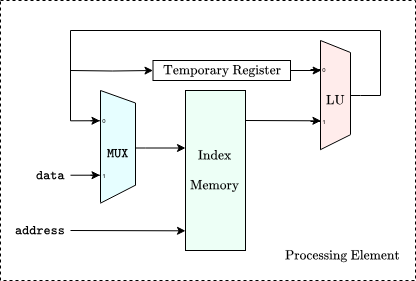
\includegraphics[width=1.0\linewidth]{body/ch3/figs/fujishima-qip-block}
	\caption[Fujishima's Processing Element for Emulating Qubits.]{The QIP processing element for emulating the parallel computing of quantum states in a quantum computer. Fujishima implemented 2048 processing elements for executing the calculations using quantum indices in the input-and-output table. \cite{fujishima2003fpga}.}
	\label{fig:fujishima-qip-block}
\end{figure}

\subsection{Representing Qubit Probabilities Using A Fixed-Point Scheme with Mantissa Bits}

Khalid, Zilic and Radecka were able to expand on the study by Fujishima by proposing a new FPGA-based emulator design that allows efficient experimentation with new quantum algorithms. Khalid et al.'s paper concentrated on new techniques for modelling quantum circuits, including entanglement and probabilistic computing realisation \cite{Khalid2004}. The primary difference between Fujishima's approach and Khalid et al.'s approach is that unlike Fujishima who used an input-and-output table, Khalid et al. considered the probabilistic nature of quantum states which leads to measurement error \cite{Khalid2004}. In addition, Fujishima's study did not include results from the synthesised circuit on a FPGA. To integrate the probabilistic nature of qubits while managing resources for emulating quantum circuits efficiently on an Altera Stratix EP1S80B956C6 FPGA, Khalid et al. used a fixed-point scheme to represent the values of the normalised amplitudes $\alpha$ and $\beta$ which represent the probability of measuring one of the basis states. To perform quantum measurements, Khalid et al. proposed that it suffices for the probabilities of detecting each state to be pre-computed in software and stored in hardware. These probabilities can be used as weights to emulate the random state detection in hardware \cite{Khalid2004}. 

Khalid et al. highlighted that a classical probabilistic circuit runs a series of inputs through the network of gates and outputs the bits according to the probability distribution induced by the network \cite{Khalid2004}. This leads to the probability of an error in measuring probabilistic circuit outputs.  Khalid et al. elucidated that the choice of a fixed-point scheme over a floating-point scheme was due to the fact that $\alpha$ and $\beta$ can have a decimal point of 0 or 1 only, as shown in the theoretical framework in section \ref{subsec:qft} \cite{Khalid2004}. Khalid et al. further elaborated that using a floating-point representation of the complex exponent does not bring benefits in this case \cite{Khalid2004}. To achieve precision, Khalid et al. used \gls{mantissa} bits in a modular way by changing the size of the fractional part without modifying other components of the system. This method is advantageous for experiments dealing with precision and fault-tolerance of quantum algorithms and incorporates the ideas of error correction to the emulator \cite{Khalid2004}. 

\subsection{Emulation Accuracy and Logic Cell Usage}

In a similar 2008 study of an FPGA-based quantum circuit emulation, Aminian et al. proposed a new representation for qubits to considerably improve the application of quantum circuits on FPGA-based emulations \cite{Aminian2008}. Aminian et al. represented complex coefficients of each qubit using fixed-point numbers with an $N$ bit \gls{mantissa}. Given that a qubit in the computational basis has two complex coefficients with two components each, four fixed-point numbers were used to represent a qubit \cite{Aminian2008}. Amina et al. noted that the emulation accuracy of the design was directly related to the number of mantissa bits for measuring the emulation efficiency. The emulation accuracy increased as the number of \gls{mantissa} bits is increased \cite{Aminian2008}.

The results from Aminian et al.'s implementation were compared to the implementation by Khalid et al. to estimate the overall improvement in the usage of logic cells when different mantissa bit-sizes were implemented. When Aminian et al. performed the emulation experiments on an Altera Stratix EPIS80B9056C6 FPGA, the results showed a higher improvement in the usage of logic cells for the implementation that uses an 8-bit mantissa \cite{Aminian2008}. Aminian et al. were particularly interested in the logic cell usage for different qubit transformations using Hadamard, phase shift, Pauli, and \texttt{CNOT} quantum gates. Experimental results showed the best improvement ($99\%$) in logic cell usage from Khalid et al.'s implementation when the \texttt{CNOT} operation was performed \cite{Aminian2008}. This improvement corresponded to employment of a 16-bit mantissa to perform the unitary matrix operation. In this case, Khalid et al.'s implementation of the \texttt{CNOT} used 375 logic cells, but Aminian et al. required only 4 logic cells in their implementation \cite{Aminian2008}.

\subsection{Representing Qubits on a Bloch Sphere To Emulate Entanglement Using VHDL}
  
In 2008, Mohamed, Badawy and Jullien, investigated how a programmable logic array could be used to practically emulate quantum computations with entanglement characteristics by extending the concept of phase and the Bloch sphere representation of qubits to classical bits on a FPGA \cite{mohamed2009using}. Mohamed et al. emphasised that apart from the initial set of quantum states and the final measured state, the hidden state of a qubit must also be stored by a classical computer in two complex fixed-point registers representing a qubit on the surface of a Bloch sphere \cite{mohamed2009using}. Assuming that a 10-bit fixed-point number representation is sufficient precision for the coefficients, then 40 bits of classical storage are required to represent the quantum state of one qubit \cite{mohamed2009using}. Mohamed et al. underscored that two parameters may be used to represent a qubit by observing that, by expressing an internal qubit state as the density matrix
\begin{align}\label{eqn:density-matrix}
	\rho	& = \frac{1}{2}\left(I + \beta_x\sigma_x + \beta_y\sigma_y + \beta_z\sigma_z\right)
\end{align}
where $\beta_x$, $\beta_y$ and $\beta_z$ are real numbers and $I$, $\sigma_x$, $\sigma_y$, and $\sigma_z$ are Pauli matrices, the spherical coordinates $r$, $\phi$ and $\theta$ could be used with $r = 1$ from the normalise constraint which requires that
\begin{align}
	\beta_x^2 + \beta_y^2 + \beta_z^2 = 1\nonumber
\end{align}
Mohamed et al. used this approach to represent a qubit as a vector on the surface of a Bloch sphere. This implementation ignored the overall phase factor of the qubit since it is not observable, even though the factor appears general mathematical representation of the coefficients in spherical coordinates given by
\begin{align}\label{eqn:qubit-spherical-coordinates}
	\alpha_0	& = e^{i\gamma}\cos(\theta/2)\\
	\alpha_1  & = e^{i\gamma}e^{i\phi}\sin(\theta/2)
\end{align}
In this form, the spherical coordinate representation of a qubit is only applicable to a single qubit quantum computer, which cannot be more useful than a single bit classical computer in terms of its computational capabilities. Recalling that for a two-qubit quantum computer, the state of the system is related by the basis vectors $\ket{00}, \ket{01}, \ket{10}, \ket{11}$, it can be observed that the internal state of two qubits requires representation by 4 complex fixed-point registers or 7 floating-point numbers \cite{mohamed2009using}. Mohamed et al. generalised this observation by suggesting that the internal state of a quantum register with $n$ qubits requires $2\times2^n - 1$ classical fixed-point registers \cite{mohamed2009using}.

While conducting experiments on a FPGA, the representation of a qubit using the angles $\theta$ and $\phi$ was achieved using LUTs for managing the $\sin$ and $\cos$ functions and manipulation of the complex coefficients $\alpha_{0}$ and $\alpha_{1}$ \cite{mohamed2009using}. This representation of qubits in spherical coordinates is suitable for the operations on the qubits that result in state vector rotations on the surface of a Bloch sphere or unit circle. According to Mohamed et al., the number of entries in the LUT is a function of the angle resolution and the number of bits per entry is a function of the required precision of the representation of the sinusoidal functions \cite{mohamed2009using}. Since the ratios produced by the sine function in the range of angles between $\pi/4$ and $\pi/2 \si{\radian}$ are the same as the ratios produced the cosine function for angles between $0$ and $\pi/4\si{\radian}$, it suffices to store 8 pairs of angles between $0$ and $2\pi\si{\radian}$. Then, by symmetry, values of the sinusoidal function in the other quandrants of the Bloch sphere or unit circle can be obtained by manipulating the sign bit in the LUT \cite{mohamed2009using}.

Extending the representation of quantum states in spherical coordinates allowed Mohamed et al. to utilise entanglement in reducing the emulation resource requirements from the correlation between the qubit states \cite{mohamed2009using}. Emulation resource requirements are typically intensive due to the probabilistic characteristics of a qubit which manifest in a superposition of states. To illustrate the large number of resources, consider a problem that can be solved using 128 qubits \cite{mohamed2009using}. For a classical computer, 128 bits can represent decimal values between 0 and $2^{128}-1$, however, to know the value, all bits must be read exactly. For a quantum computer with 128 qubit registers, all $2^{128}$ states can be represented simultaneously, which would require 128 address bits for emulation on a classical computer \cite{mohamed2009using}. Additionally, the classical computer would need to update all the memory space at every step due to qubit entanglement \cite{mohamed2009using}. 

In a closed system, qubit entanglement does not increase storage requirements since a correlation between quantum states is initiated when Bell states are created \cite{mohamed2009using}. To emulate quantum entanglement, Mohamed et al. suggested that the classical platform needs to keep track of the entangled qubits and update their states after every operation \cite{mohamed2009using}. Mohamed et al. successfully used this approach to emulate the solution path of the Deutsch-Jozsa algorithm which uses the QFT to determine whether a single bit black box function $f(x)$ is a constant function or not \cite{mohamed2009using, Nielsen2010}. The architecture of their proposed system was implemented using VHDL which defined a fixed-point library with complex class storage, a complex multiplier and an approximation of the multiplication by the factor of $1/\sqrt{2}$ \cite{mohamed2009using}. An approximation needs to be used since $\sqrt{2}$ is an irrational number. This approximation was achieved using a series of shifts and additions while the complex multiplier was performed in a strength reduced form which required three real multipliers instead of four at the expense of extra adders \cite{mohamed2009using}. Storage of fixed-point numbers was defined as a typed derived from standard logic \cite{mohamed2009using}. The VHDL code was written based on a set of generic parameters which defined the number of qubits and the number of operations \cite{mohamed2009using}. 

\subsection{Representing Qubit State Vectors in a Unit Circle Using Quantum Cells}

Valerii Hlukhov described a digital quantum computer, in 2020, as a device that consists of a classical processor and a digital quantum coprocessor as shown in figure \ref{fig:hlukhov-digital-qc} \cite{Hlukhov2021}. Considering that many modern FPGA system chips come with integrated processors, Hlukhov proposed that the control unit, for example a 32-bit ARM RISC processor, could be used to determine the initial state of the $j^\text{th}$ qubit in the system input \cite{Hlukhov2021}. In their study, experiments were conducted on a ZedBoard Zynq-7000 ARM\_FPGA SoC Development Board using Xilinx Zynq-7000 AP SoC XC7Z020-CLG484 at $\SI{100}{\mega\hertz}$ \cite{Hlukhov2021}. The control unit also determines a set of instructions for each of the digital quantum cell or qubit, as well as the necessary data for each this instruction set \cite{Hlukhov2021}. Static connections between digital qubits were facilitated by the switching matrix which also provided the results to the control unit \cite{Hlukhov2021}.

\begin{figure}[!ht]
	\centering
	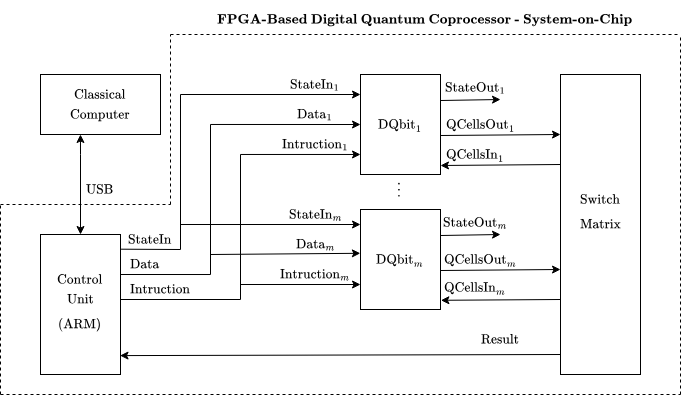
\includegraphics[width=1.0\linewidth]{body/ch3/figs/hlukhov-digital-qc}
	\caption[Generalised Functional Diagram of an Emulated Digital Quantum Computer by Hlukhov.]{A digital quantum computer consists of a control element for initialising quantum states (\texttt{StateIn}\_j corresponding to the digital qubit labelled \texttt{DQbit}\_j). The switching matrix connects qubits to each other and returns the results to the control unit on the FPGA.}
	\label{fig:hlukhov-digital-qc}
\end{figure}

Hlukhov also defined a \textit{digital qubit} as a qubit that can be represented as a discrete finite state machine resulting from a unique chain of quantum gates \cite{Hlukhov2021}. Hlukhov's study focused on implementing the FPGA-based digital quantum coprocessor consisting of 4 to 128 qubits capable of performing the QFT. Each digital qubit consisted of a $j$ series-connected digital quantum cells describing a single operation that transforms the state code \texttt{State} of the measured state $\ket{Q_{0j}}$ as shown in figure \ref{fig:hlukhov-qubit} \cite{Hlukhov2021}. The state of qubits was conditionally described as $\ket{x_mx_{m-1}...x_1x_0}$, where each $x_j$ corresponds to the neutral position of the state vector in the unit circle at an angle of $\theta$. The movement of this state vector in the unit circle corresponds to the behaviour of a single qubit with real amplitudes of the probabilistic quantum state \cite{Hlukhov2021}. Hlukhov chose the polar coordinate system to represent the position of the vector in contrast to the Cartesian coordinate system which requires two values for the input and the output \cite{Hlukhov2021}. 

\begin{figure}[!ht]
	\centering
	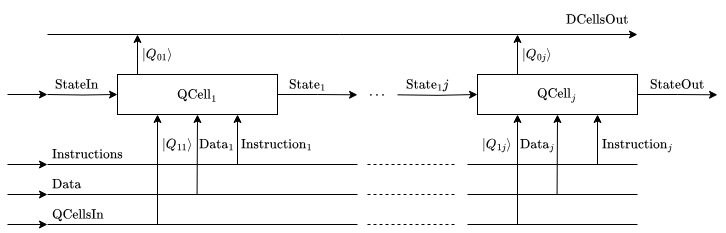
\includegraphics[width=1.0\linewidth]{body/ch3/figs/hlukhov-qubit}
	\caption[Digital Qubit (DQbit) by Hlukhov.]{Hlukhov's digital quantum qubit (DQbit) consists of quantum cells (QCell) that receive the initial state $StateIn$, instructions and data from the external control unit \cite{Hlukhov2021}.}
	\label{fig:hlukhov-qubit}
\end{figure}

The quantum cells were arranged such that the first cell in the series receives the initial state code from the external control unit and the last cell in the series stores the status code of the final qubit state in an output pipeline register \cite{Hlukhov2021}. Additionally, each quantum cell receives the measured state $\ket{Q_{1j}}$ of another qubit from the switch matrix \cite{Hlukhov2021}. The probabilistic nature of quantum measurements of qubits was enabled by a pseudo-random number generator in the measuring unit facilitated by the FPGA ROM \cite{Hlukhov2021}. 

The pseudo-random number generator produced values such that in the switch matrix, the probability of measuring input states in the computational basis with an odd parity of bits was equal to the probability of measuring state codes with even parity \cite{Hlukhov2021}. In other words, Hlukhov distributed the probability of measuring each state according to the parity of state code in the computational basis. The results from the experiment using digital qubits in this manner on the FPGA-based digital quantum coprocessor showed that the execution time of the QFT does not depend on the number of qubits in the coprocessor and is commensurate with the decoherence time of electron-spin-based qubits, i.e. about $\SI{10}{\nano\second}$ \cite{Hlukhov2021}. For instance, the results showed that the percentage of FPGA resources used when 10 qubits were emulated was $24\%$ and when 128 qubit digital quantum coprocessor was emulated, the resource usage percentage decreased to $14\%$ \cite{Hlukhov2021}.

In summary, careful consideration needs to be taken on the representation qubits as classical bits in the FPGA-based quantum computer emulation. The manner in which qubit quantum states are stored in memory is critical for the precision of the emulation. Furthermore, streamlining the definition of a quantum state is crucial for the performance of the design. Literature shows that the emulation time grows exponentially as the number of bits $n$ increases, however, when the representation of qubits is carefully selected, the percentage of FPGA resources that are used to emulate qubits can be independent of the number of qubits \cite{Hlukhov2021, hong2022quantum}. The following section provides a review on how quantum gates and quantum circuits are performed classically to emulate a quantum computing algorithms on a FPGA. 
%such as the Bell state given by 
%\begin{align}
%	\ket{\psi} & = \alpha_{00}\ket{00} + \alpha_{01}\ket{01} + \alpha_{10}\ket{10} + \alpha_{11}\ket{11}
%\$end{align}

\section{Emulating Quantum Gates and Quantum Circuits on FPGAs \label{sec:lit-fpga-qgate-qcircuit}}

FPGA architectures depend on the constraints of logic element structures, programmable interconnect structures, interconnection networks, configuration, and different types of wires, including local, global and general purpose wires \cite{wolf2004fpga}. Programmable logic blocks and programmable interconnects provide multi-level logic and parallelism which is suitable for the emulation of quantum gates and their effect on qubits in a quantum circuit. Efficient use of the resources on the FPGA can allow quantum algorithms to be emulated in a shorter time by sequence of quantum gate operations is performed appropriately based on the constraints of the device. The most commonly implemented is the QFT due to its applicability in various quantum algorithms as described in the theoretical framework in chapter \ref{ch:theoretical_framework}. 

\subsection{Implementing Gates to Solve a Problem Function}

Using the input-and-output table described in the previous section, Fujishima emulated the QFT to solve an NP-complete for periodic function $f(x)$ in polynomial time. In order to apply the QFT, the outputs of the table must be periodic, otherwise Grover's algorithm is used to search for a specific value from the table \cite{fujishima2003fpga}. To generate the table in polynomial time, Fujishima applied the \textit{satisfiability} problem which finds a group of variables that satisfy a given Boolean equation \cite{fujishima2003fpga}. Fujishima used the FPGA emulator to execute a satisfiability algorithm for the Boolean equation given by
\begin{align}
	(\bar{a}+c+\bar{d})\cdot(\bar{b}+\bar{e})\cdot(a+d+\bar{f}+h)\cdots(k+g)=1\nonumber
\end{align}
At the start of the emulation, the outputs corresponding to all variables were initialised to 0 by applying De Morgan's laws and negating both sides of the above satisfiability equation. The terms in the brackets of the equation were divided into nodes. In the final stage, binary search was used to investigate the input corresponding to the output with 0 to obtain the answer \cite{fujishima2003fpga}. 

\subsection{Emulating Quantum Gate Operations Using a Logic Cells}

Using a more conventional approach to emulating quantum operations on qubits, Khalid et al. developed a VHDL library of common quantum gates comprising of the Hadamard, \texttt{CNOT}, \texttt{X}, \texttt{Z} and phase shift gate \cite{Khalid2004}. In addition to using VHDL for mapping the quantum gates to code, Khalid et al. employed the code generating capabilities of VHDL to automatically produce descriptions of multiple input quantum gates from single-input gates \cite{Khalid2004}. This is in line with Barenco et al.'s observation that multi-qubit gates can be constructed using a series of single-qubit Pauli-gates and \texttt{CNOT} gates. Intuitively, single-qubit gates required less resources than the other gates. Controlled gates were initialised by passing the number of control variables as a parameter to the code generating script which produced the VHDL description of the resulting transformation \cite{Khalid2004}. This procedure allowed Khalid et al. to automate the construction of arbitrary size quantum gates using clock synchronised quantum state registers (QSR) that can represent the state of the quantum system at any given stage in the flow of data \cite{Khalid2004}. Gates that produce entangled states required considerably more resources than gates where no entanglement occurred due to \cite{Khalid2004}. Figure \ref{fig:khalid-q-evo} illustrates the emulation of quantum evolution of an entangled system for the case of two qubits $\psi_1$ and $\psi_2$ that are used as the control and target qubit of the \texttt{CNOT} gate. In this case, the \texttt{CNOT} gate requires 4 complex multiplications \cite{Khalid2004}. In general, a $n$ input \texttt{CNOT} gate requires $2^n$ complex multiplications \cite{Khalid2004}. Khalid et al. noted that this exponential increase in resource requirement for emulating entanglement poses a fundamental bottleneck in modelling quantum systems by classical means \cite{Khalid2004}. 

\begin{figure}[!ht]
	\centering
	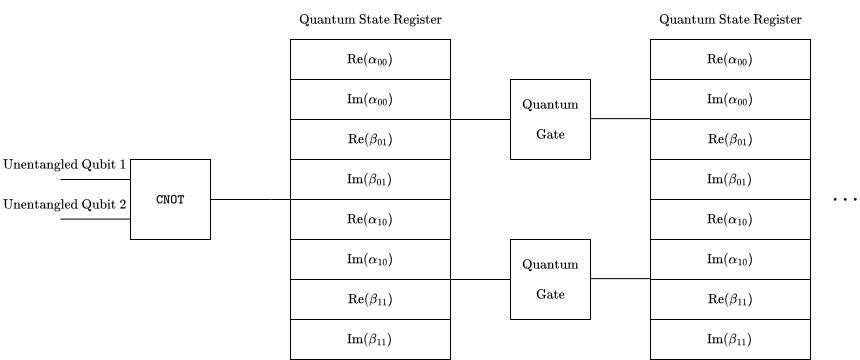
\includegraphics[width=1.0\linewidth]{body/ch3/figs/khalid-q-evo}
	\caption[Showing Use of Quantum Registers in a Quantum Circuit Evolution by Khalid et al.]{Quantum state registers represent the state of the entire system at a given stage in the evolution of a quantum circuit \cite{Khalid2004}.}
	\label{fig:khalid-q-evo}
\end{figure}

Khalid et al. successfully used logic cells for quantum gates in the VHDL library to emulate the quantum circuits associated with the QFT and Grover's search algorithm for a 4 element database using 3-qubits \cite{Khalid2004}. The most commonly used quantum gate was the Hadamard gate. In the case where 16-bit mantissas were used to achieve a higher emulation accuracy, 1284 logic cells were used to emulate Hadamard gate operations on an Altera Stratix FPGA \cite{Khalid2004}. About 580 less logic cells were required to achieve a lower emulation accuracy using 8-bit mantissas for the same operations using the Hadamard gate \cite{Khalid2004}. Khalid et al. highlighted that since $X$ and $Z$ gates do not use logic cells because the swap and bit flip operations performed consume negligible resources \cite{Khalid2004}. The same clock speed of $\SI{82.1}{\mega\hertz}$ was used to emulate the QFT and Grover's search algorithm using the logic cell quantum gates. However, Grover's search algorithm used more logic cells in total. While emulating the 3-qubit QFT with 16-bit mantissas used 5076 logic cells in total, emulating Grover's search algorithm consumed 12636 logic cells. 

\subsection{Emulating Quantum Gates that Produce Entangled States}

The proposed method by Aminian et al., which employed fixed-point numbers to represent the normalised coefficients as described in the previous section, also implemented the $X$, $Z$, \texttt{CNOT}, phase shift and Hadamard gate. However, the main difference between Khalid et al. and Aminian et al.'s implementation of these universal quantum gates is that instead of using QSRs to represent the stage of evolution of the quantum states, Aminian et al.'s FPGA emulated Pauli and controlled gates were implemented using three additional bits labelled $b$, $i$, and $s$, corresponding to the basis, complexity and sign \cite{Aminian2008}. To emulate Pauli gate operations, the bits were manipulated as illustrated in figure \ref{fig:aminian-pauli-gates}. Similar to Khalid et al.'s implementation, Aminian et al.'s design required more computational resources for emulating quantum entanglement \cite{Aminian2008, Khalid2004}. For example, applying the single-qubit Hadamard gate on a single qubit required four multipliers and four adders, while applying the same gate on three entangled qubits $\ket{j_1 j_2 j_3}$ required sixteen multipliers and sixteen adders \cite{Aminian2008}. 
\begin{figure}[!ht]
	\centering
	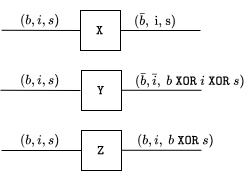
\includegraphics[width=0.75\linewidth]{body/ch3/figs/aminian-pauli-gates}
	\caption[Implementation of Paul-$X$, $Y$, and $Z$ Gates by Aminian et al.]{Using the bits to represent the basis ($b$), the complexity ($i$) and sign ($s$), Aminian et al. were able to implement the single-qubit Pauli gates showing above \cite{Aminian2008}.}
	\label{fig:aminian-pauli-gates}
\end{figure}

To emulate the \texttt{CNOT} gate, additional qubits were appended to the entangled bit $b$ in the computation basis. Hadamard and controlled-$R$ gates, were implemented in a similar manner to Khalid et al.'s implementation where intermediate QSRs are used to keep track of the quantum states of the quantum computer \cite{Aminian2008, Khalid2004}. When both groups of gates were used, the gate operations were implemented by a coefficient swapping operator \cite{Aminian2008}. In this case, the $X$ gate was implemented with four registers and the $Z$ gate was implemented by multiplying the $\beta$-coefficient of the quantum state by -1 \cite{Aminian2008}. Aminian et al. designed the emulation method using VHDL and evaluated various library gates in both distinct and entangled 3-qubit states for performing the QFT and Grover's search algorithm \cite{Aminian2008}. Aminian et al.'s method used significantly less logic cells on the Altera Stratix FPGA compared to Khalid et al.'s implementation on the same board. For example, when using 16-bit mantissas to perform the QFT, Khalid et al.'s implementation required only 8197 logic cells compared to the 12636 logic cells required in Khalid et al.'s emulator \cite{Aminian2008, Khalid2004}. However, Aminian et al.'s synchronised each block of the emulation stage using a higher clock frequency of $\SI{131.3}{\mega\hertz}$ \cite{Aminian2008}. 

\subsection{Adjusting State Machine Corresponding to Unitary Operations}

Mohamed et al.'s implementation of two angles from the spherical coordinates of the quantum state of qubits used a state machine in VHDL to calculate the matrix tensor products in the Deutsch-Jozsa algorithm. The size of the matrix tensor products was determined by the total number of qubits in the quantum computer \cite{mohamed2009using}. VHDL blocks adjusted the state machine in order to produce the tensor product operation matrix associated with 3 Hadamard gates and one \texttt{CNOT} gate. The overall design flow proposed by Mohamed et al. for hardware acceleration using an FPGA are shown in figure \ref{fig:mohamed-design-flow} where the VHDL generation step refers to connecting the chain of operations after setting up the generic parameters which define the number of qubits and the number of operations \cite{mohamed2009using}. 

%TODO
%Mohamed-design-flow


\subsection{Quantum Fourier Transform Implementations using DSP Blocks}

Rivera-Miranda, Caicedo-Beltr\'{a}n, Valencia-Pay\'{a}n, Espino-Duran, and Velasco-Medina addressed the shortcomings of software simulators by presenting a hardware design of an emulator for computing the QFT using FPGAs in 2011 \cite{rivera2011hardware}. The proposed hardware design methodology differs from the ones by Fujishima, Khalid et al., Aminian et al. and Mohamed et al. in that it used a fixed-point two's complement representation with 2 bits in the integer part. Instead of matrix operations which would require a lot of hardware resources, Rivera-Miranda et al. designed quantum gates using building blocks, with sum, subtract or multiply only when it is necessary \cite{rivera2011hardware}. For example, similar to the implementation by Aminian et al., the Hadamard gate used four multipliers and four adders, whereas the controlled phase shift or controlled-$R$ gate required four multipliers and two adders as illustrated in the block diagrams in figure \ref{fig:rivera-hadamard-gate} \cite{rivera2011hardware}. This architecture of these quantum gate emulations was described in VHDL where the user parameters were the number of qubits, the number of mantissa bits and the pipeline depth \cite{rivera2011hardware}. 

The operation of the circuit was successfully verified over two clock cycles using ModelSim-Altera to simulate a 4-qubit quantum computer using a 16-bit mantissa to improve computational accuracy \cite{rivera2011hardware}. On the first cycle of the simulation, the given input state, \textit{iqubit} was $\ket{j} = \ket{0111}$ and on the second cycle, the output signal \textit{oqubit} was the quantum state $\ket{y} = \ket{y_1 y_2 y_3 y_4}$, where
\begin{align}
	y_1	 & = 0.7071\ket{0} - 0.7071\ket{1}\nonumber\\
	y_2	 & = 0.7071\ket{0} - j0.7071\ket{1}\nonumber\\
	y_3	 & = 0.7071\ket{0} + (-0.5000 + j0.5000)\ket{1}\nonumber\\
	y_4	 & = 0.7071\ket{0} + (-0.2706 + j0.6533)\ket{1}\nonumber
\end{align}
which corresponds to the expected transformation at the end of the QFT quantum circuit \cite{rivera2011hardware}. Rivera-Miranda were able to synthesise the design on the Altera Stratic FPGA as depicted in the block diagram in figure \ref{fig:rivera-block-diagram} using the Quartus II Professional software suite \cite{rivera2011hardware}. The diagram includes a multiplexer at the parallel output which was used to present the resulting qubits one-by-one once all the input qubits had been loaded and after a number of cycles given by the latency \cite{rivera2011hardware}. 

%TODO
%Rivera 

Another difference in Rivera-Miranda's implementation is that the QFT was implemented using Altera's IP cores that use mainly 18-bit DSP blocks and the distributed memory bits to reduce the number of hardware resource required \cite{rivera2011hardware}. Results from the synthesis of the QFT on FPGA were summarised into the number of adaptive LUTs, registers and DSP blocks. These results showed a linear increase in the number adaptive LUTs and registers while there were available DSP blocks, and an exponential increase when there were not available DSP blocks \cite{rivera2011hardware}. To emulate 16-qubits, 14786 adaptive LUTs, 3537 logic registers, 768 9-bit DSP blocks were employed at a maximum clock frequency of $\SI{83.10}{\mega\hertz}$ \cite{rivera2011hardware}. The clock frequency decreased as the number of qubits in the emulated quantum computer increased.

\subsection{Concurrent vs Sequential Implementations of Quantum Gate Operations}

More recently in 2014, Lee, Khalil-Hani and Marsono conducted experiments based on the QFT to identify suitable qubit representation and hardware design techniques for manage resources that grow exponentially as the number of qubits in the system grows \cite{lee2014fpga}. Lee et al. suggested that the QFT is a suitable candidate as an entry-level case study for quantum circuit emulation because it can be easily mapped into a simple quantum circuit \cite{lee2014fpga}. Furthermore, Lee et al. distinguished between concurrent, pipelined, and serial processing for emulating quantum circuit classically. Concurrent processing allows parallelism which completes all computations within on clock cycle while pipeline processing includes additional registers as illustrated in figure \ref{fig:lee-concurrent-v-pipeline} \cite{lee2014fpga}.

\begin{figure}[!ht]
	\centering
	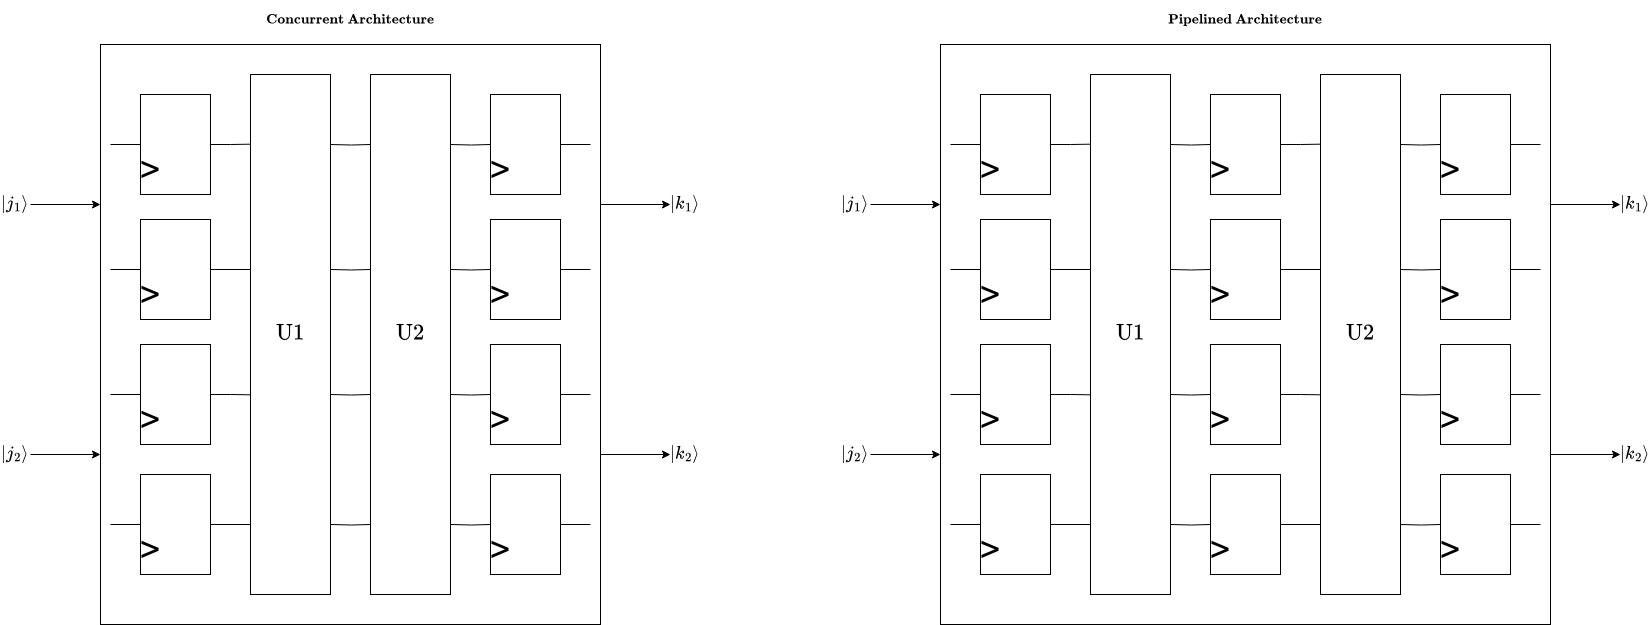
\includegraphics[width=1.0\linewidth]{body/ch3/figs/lee-concurrent-vs-pipeline}
	\caption[Side-by-Side Comparison of Concurrent and Pipelined Emulation by Lee et al.]{Concurrent emulation (left) allows for parallelism in that all the quantum gate operations are performed before the output states are produced. A pipelined design (right) is more suitable for producing high throughput with low critical path delays due to the insertion of registers after each stage of the unitary transformation \cite{lee2014fpga}.}
	\label{fig:lee-concurrent-v-pipeline}
\end{figure}

Although a concurrent technique can allow parallelism and effective resource management, Lee et al. noted that this would lead to a high critical path delay and low operating frequency \cite{lee2014fpga}. The advantage of using a serial architecture is that it increases throughput and decreases the critical path delay while presenting the designer with the opportunity to utilise resource sharing through shared registers as illustrated in figure \ref{fig:lee-serial-architecture} \cite{lee2014fpga}. The results also showed that a serial design achieves balance on both resource utilisation and operating frequency as the number of dedicated logic registers in the serial architecture was reduced for a constant operating frequency \cite{lee2014fpga}. Additionally, the experiments showed that a 16-bit fixed-point representation introduced significant precision error for both 2-qubit and 5-qubit QFT emulations \cite{lee2014fpga}. The precision error of the 2-qubit QFT was successfully reduced to zero by expanding the number of mantissa bits up to 22 bits, or a total of 24 bits \cite{lee2014fpga}.

\begin{figure}[!ht]
	\centering
	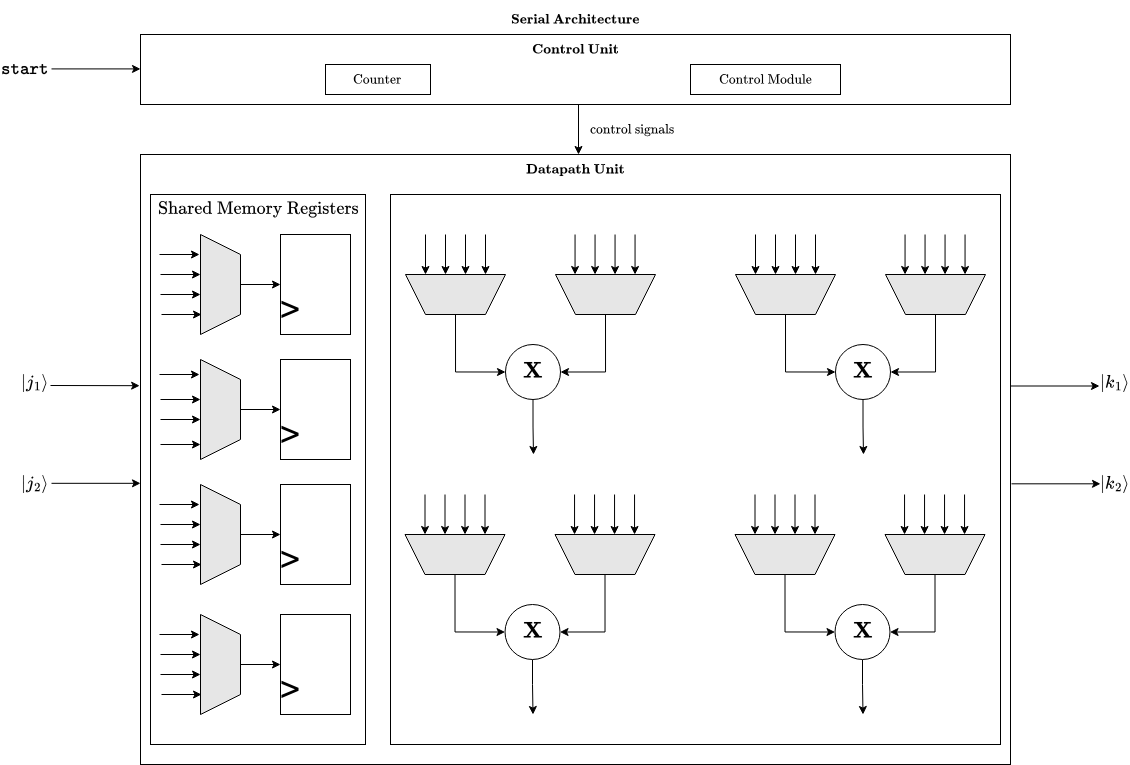
\includegraphics[width=1.0\linewidth]{body/ch3/figs/lee-serial-architecture}
	\caption[Serial Architecture of Emulated Quantum Computer by Lee et al.]{The following diagram illustrates the serial architecture for a 2-qubit quantum computer emulator. Although the serial architecture may require more iterations than the concurrent and pipelined architectures, it offers resource sharing which can be considerably beneficial in terms of resource management \cite{lee2014fpga}s. Here, the multiplication symbols illustrate the product of the inputs with the probabilistic coefficients.}
	\label{fig:lee-serial-architecture}
\end{figure}

However, the short-coming of this implementation is that it does not consider the coupling of qubits, as required by DiVincenzo's criterion regarding well-characterised qubits. 

\subsection{Emulated Quantum Gate }
 
The study focused on implementing the digital quantum coprocessor on FPGA to factorise the integer $(15)_{10}$ using Shor's algorithm. To emulate quantum gates in the FPGA-based digital quantum computer, Hlukhov began by distinguishing between a quantum gate in an analog quantum computer and a digital quantum gate in a digital quantum computer \cite{hlukhov}. Hlukhov took a quantum gate in an analog quantum computer to only symbolise the operation of changing the position of a vector on a Bloch sphere or in a unit circle \cite{Hlukhov2021}. In contrast, a digital quantum gate in a digital quantum computer was taken to represent a digital device that changes the internal code of a qubit as a finite state machine, corresponding to a change in the intermediate position of a single vector on a Bloch sphere or in a unit circle \cite{Hlukhov2021}. Similar to previous implementations that used pipeline QSRs, Hlukhov introduced a model of digital quantum gate that includes an ALU, a comparator and a pipeline register as seen in figure \ref{fig:hlukhov-qgate} \cite{Hlukhov2021}. 

\begin{figure}[!ht]
	\centering
	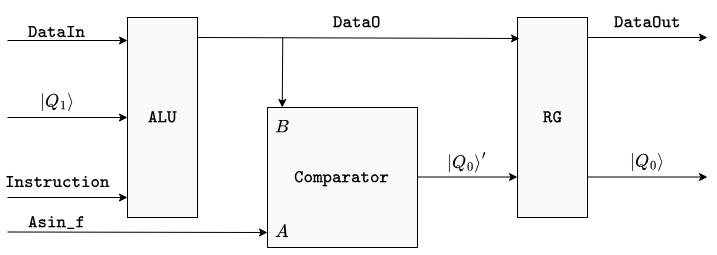
\includegraphics[width=1.0\linewidth]{body/ch3/figs/hlukhov-qgate}
	\caption[Proposed Quantum Gate by Hlukhov.]{Model of a digital quantum gate that includes an ALU, a comparator and a pipeline.}
	\label{fig:hlukhov-qgate}
\end{figure}

In the digital quantum gate model, the output of the gate is represented by the qubit state code \texttt{DataOut} and the measured state $\ket{Q_0}$ of a qubit is taken from the pipeline register \cite{Hlukhov2021}. An intermediate status code, \texttt{DataO}, is evaluated in the comparator with the random variable \texttt{Asin\_f} to obtain the measured state $\ket{Q_0}'$. The only types of quantum gates that were emulated using this implementation were the Hadamard and the controlled phase shift gates. After performing the QFT, the expected output was $80000000_{16}$, corresponding to the number of periods \cite{Hlukhov2021}. It was shown that the probability of obtaining true results increases rapidly with a decrease in the state code length \cite{hlukhov2021digital}. 

\subsection{Memory Considerations for Emulating Quantum Gates}

In 2022, Hong, Jeon and Park proposed a hardware architecture which operates based on a single-input gate regardless of the number of qubits used in the circuit \cite{hong2022quantum}. The proposed architecture was implemented on a FPGA using an Advanced Peripheral Bus (APB) interface for setting parameters such as gate data and an Advanced High-performance Bus (AHB) interface for communication with external memory \cite{hong2022quantum}. The aim of the implementation was to reduce unnecessary multiplications and data transfer with SDRAM external memory \cite{hong2022quantum}. The QFT quantum circuit was emulated in three stages, with each gate performed in the circuit one by one. 

In the first stage, state grouping was performed using the characteristic that an element of the output state vector, which applied by a single-qubit gate, is only affected by two elements of the input state vector \cite{hong2022quantum}. Since a single-qubit gate is only applied to one qubit, it cannot modify the state of the other qubit in the group. At the end of the state grouping stage, pairs of states were sent to the second stage where unnecessary data transfer from external memory was eliminated \cite{hong2022quantum}. This is performed by skipping data transfer if an element of the output state does not change from that of the input state \cite{hong2022quantum}. Furthermore, control-gates were skipped when the control-bit was 0 since states are only transformed when the control qubit is 1 \cite{hong2022quantum}. Hong et al. reported that using this scheme, half of the output states can be skipped to reduce multiplication operations and data transfer from external memory \cite{hong}. In the final stage of the finite state machine describing the implementation, matrix elements of the input state vector were multiplied by the $2\times2$ unitary matrix of the quantum gate. The output state was produced using the grouped states from the first stage. 

Hong et al.'s architecture was synthesised and emulated on a Xilinx Kintex UltraScale (XCKU115) FPGA platform at $\SI{160}{\mega\hertz}$. The implementation used 19204 LUTs, 4027 registers and 128 DSP blocks \cite{hong2022quantum}. In addition, the architecture used a 16-bit fixed point precision for representing data, equating to a total of 32 bits used for storing a single complex number corresponding to a state vector \cite{hong2022quantum}. Experimental results showed that emulation time grew exponentially as the number $n$ of qubits increased, according to the dimensions of the quantum state vector \cite{hong2022quantum}. 

\section{Testing and Benchmarking the Performance of FPGA-Based Quantum Computer Emulators}

In most of the literature explored above where quantum computers have been emulated on FPGAs, the design is evaluated by comparing resource usage and execution times with previous implementations. For example, Aminian et al. use the results from Khalid et al.'s implementation to compare the total number of logic cells required by the design \cite{Aminian2008, Khalid2004}. As quantum computing operations involve dense matrices, careful consideration must be taken regarding testing and benchmarking the performance of the FPGA design. 

In 2024, Lee Belfore II proposed a scalable accelerator architecture specifically to solve the challenge of managing parallelism by efficiently routing quantum state components for gate evaluation and measurement \cite{belfore2024scalable}. Belfore demonstrated the architecture on an Intel Agilex AGFB014 FPGA on the Intel Agilex F-series FPGA development kit using a fixed-point scheme. Belfore noted that in order to support high performance data processing, DSPs can provide optimised and flexible multipliers, adders, and registers that facilitate high speed operation and efficient pipeline \cite{belfore2024scalable}. Subsequently, memory in the vicinity of DSP blocks reduce latencies incurred by sourcing operands. Belfore identified the usefulness of ARM based processor cores, that many FPGAs offer, in coordinating high level operation and tasking \cite{belfore2024scalable}. 

According to Belfore, since algorithms on FPGAs can be implemented by mapping an algorithm to a state machine this implemented directly on the FPGA, the state machines can be organised heirarchically in order to manage high level states related to phases of the computation and low level state machines that are synchronised on a clock cycle \cite{belfore2024scalable}. State machines can be implemented using Verilog which can simulate the evolution of qubits in a quantum circuit using a testbench. In their study, Belfore implemented the quantum emulator at the RTL level using the IEEE 2008 standard release of VHDL. A simple circuit consisting of a layer of Hadamard gates was simulated using the open-source VHDL platform GHDL \cite{belfore2024scalable}. 

Belfore used permutations of the inputs to align quantum state register elements to functional units on the FPGA \cite{belfore2024scalable}. Furthermore, Belfore stated that accessing the state vector in the quantum state register needs to be conducted linearly on a classical computer, therefore retrieving and operating on any component requires $\mathcal{O}(2^n)$ time \cite{belfore2024scalable}. One of the suggested improvements to the slow read and write operations is to use non-blocking permutation networks which require $\mathcal{O}(\log n)$ switching layers \cite{belfore2024scalable}.

The operation of the quantum emulator was verified by comparing results with the QuEST quantum computing simulation platform \cite{belfore2024scalable}. Belfore found that the standard deviation between the empirically derived probability distributions was $1.21\times10^{-4}$, and a mean absolute error of $1.36\times10^5$, which suggested a good agreement between the FPGA-based quantum emulator and the QuEST simulator \cite{belfore2024scalable}. Additionally, Belfore evaluated the performance of the FPGA emulator by reporting the required clocks per individual circuit emulation, clock period, and the time required for an individual emulation \cite{belfore2024scalable}. In total, results showed that the emulation time on the Intel Agilex FPGA was $\SI{14}{\micro\second}$, while the random circuit simulation using QuEST on a XEON ES-2603 v2 $\SI{1.8}{\giga\hertz}$ processor required $\SI{5.25}{\milli\second}$ of CPU time - equating to a performance speedup of 368 using the FPGA \cite{belfore2024scalable}.


%@@@@@@@ Chapter 4 - Methodology @@@@@@@@@@@@@@@@@@@@@@@@@@@@@@@@@@@@@@@@@@@@@@@@@@@@@
%This chapter starts off with details of the requirements analysis for the library of SDR IP blocks. It then goes on to discuss the design process and operational design for the proposed library. Thereafter, it describes both hardware and software tools that will be used in order to pave the way for the best development and testing environment. Then the final section overviews the experimental test for each of the designed IP blocks.
\chapter{\label{ch:methodology} Methodology}

\section{Methodology Outline \label{sec:method-outline}}

Quantum computers offer considerably more powerful computing capabilities in comparison to classical computers. However, challenges in realising qubits with long enough decoherence times make quantum computing platforms make them difficult to implement, and therefore exorbitantly expensive to manufacture and maintain. To circumvent some of the challenges that arise with building physical quantum computers, simulations and emulations of quantum computers that are modelled using classical bits offer more accessible and affordable solutions for testing useful quantum algorithms. In this paper, the design of a FPGA-based quantum computer emulator is proposed. In particular, the design is focused on emulation of the 3-qubit QFT quantum circuit and its application in the quantum factoring algorithm, as well as implementation of Grover's search algorithm in finding the index of an entry in a database with 4 elements. Notably, applications of quantum circuits in quantum algorithms require careful consideration of the quantum gate operations corresponding to unitary matrices that transform qubit state vectors. This requirement is due to the fact that as the number of qubits $n$ increases, computational resources that are necessary for simulating the $2^n \times 2^n$ dense matrices increase exponentially. 

Although CPU and GPU-based quantum computer simulations exists, the intrinsic parallelism and customisability offered by FPGAs can greatly improve the design and implementation of these types of simulations. Furthermore, parallelism of CPU and GPUs is limited by the number of cores which can run different threads in a pool to perform computations, whereas FPGA allow designers to specify combinational logic in hardware to reduce latency while producing the correct output of a quantum algorithm. Programmable logic blocks and wire networks in the FPGA fabric facilitate fine-grained parallelism which can be used to implement properties of qubits such as superposition by performing multiple operations simultaneously. Lastly, CPU and GPU-based simulations may become resource intensive and require a lot of memory and processing power to model quantum gates in a quantum circuit. 

In addition to the emulation of quantum algorithms using the logic blocks of FPGAs as quantum gates, a method for simulating a quantum interface for initialising and transmitting single-photon qubits in quantum communication protocols is developed to model the use of quantum dots for exciton emissions. Simulations of single-photon qubit behaviours that satisfy Divincenzo's criterion are performed on a microcontroller that initialises qubits on the FPGA through a light sensing interface that models exciton emissions due to incident laser pulses on a GaAs quantum dot using LEDs, BJTs and LDRs on a veroboard circuit. 

The no-cloning theorem that prohibits the duplication of quantum states makes quantum computing techniques suitable for performing secure communications. Of interest to this study is the application of quantum interfaces for initialising qubits and performing QKD through a quantum protocol that allows a sender, Alice, to transmit secure data through a quantum channel to a receiver, Bob. In this communication schema, the sender Alice, is represented by the microcontroller, while the receiver Bob, is represented by the FPGA. On the microcontroller, qubits and their operations are modelled using C language, while quantum computer operations are synthesised to hardware using VHDL. 

This chapter provides an overview of the research methodology and the different phases in the design process. The methodology is summarised in an overview diagram, followed by an in-depth description of the FPGA emulator system design and the simulation of the quantum interface using an ARM-based STM32 microcontroller. Sections detailing the research methods employed and the phases of the research project precede the system requirement analysis of the quantum emulator and quantum interface. Following the system analysis, a solution is proposed with a description of the design process and operational design for the quantum emulator. Thereafter, the chapter describes both hardware and software tools that will be used in order to efficiently design and synthesise the quantum simulation in the fabric of the FPGA. In the final section, an overview of the experimental test for each of the subsystems is provided. 

\subsection{Phases in the Research and Design Process \label{subsec:method-phases}}

The four phases of the iterative design and research methodology are illustrated in figure \ref{fig:methodology-phases} below. In the first phase, initial system requirements regarding FPGA simulation of quantum computers and the input and output data that is transmitted in quantum interfaces that facilitate communication through a quantum channel were defined. From the design brief, system requirements included PC-based software that can be used to send and receive data for processing in the emulated quantum computer.    
\begin{figure}[!ht]
	\centering
	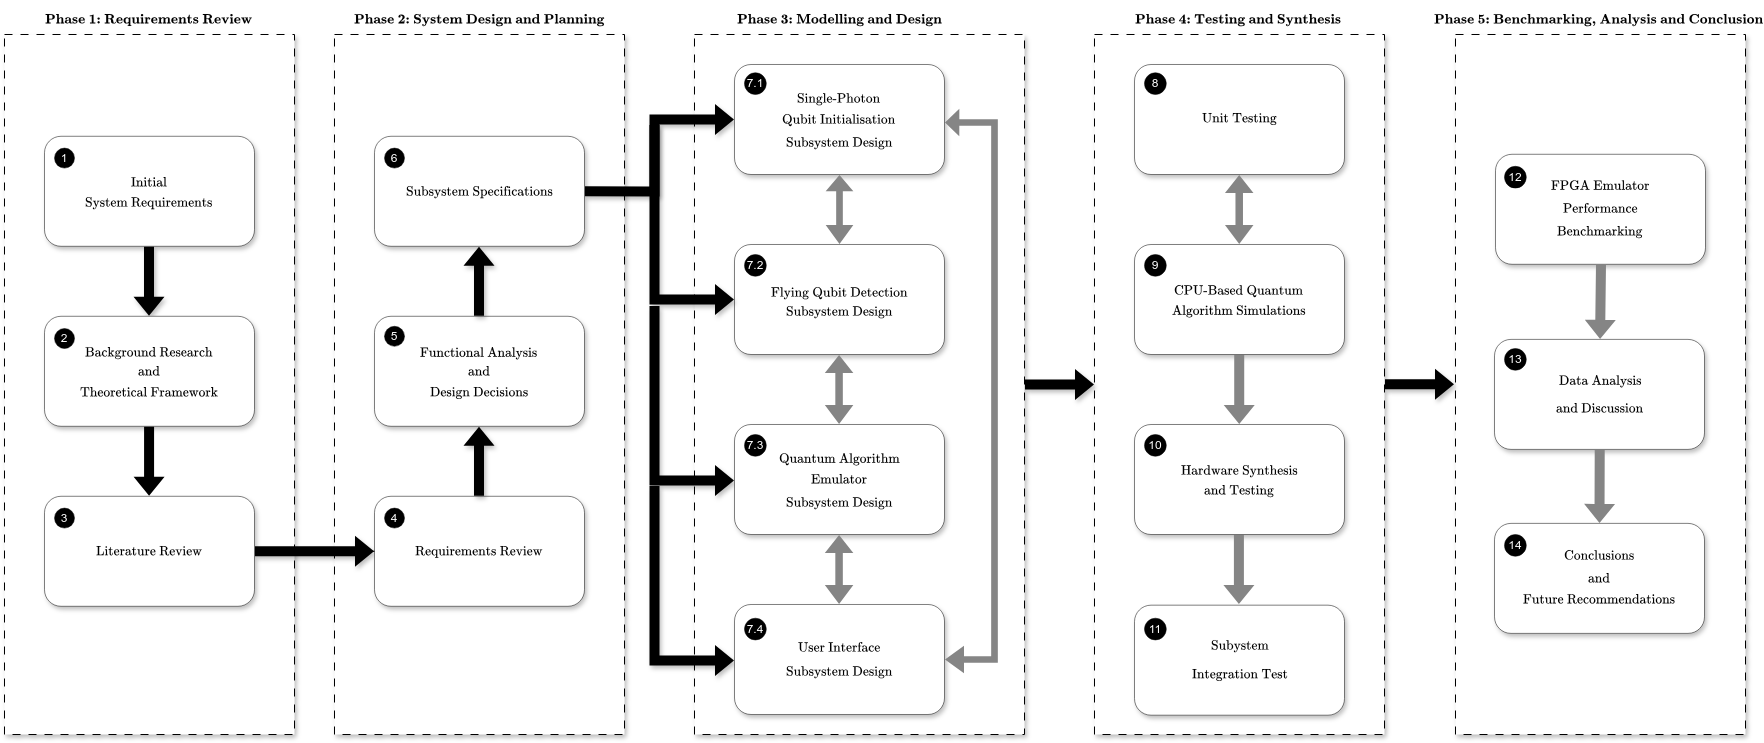
\includegraphics[width=1.0\linewidth]{body/ch4/figs/methodology-phases}
	\caption[Methodology Overview Diagram.]{Methodology overview diagram showing the four phases of the iterative design process, with each step indicated by a block and the direction of flow of critical data between steps presented by the arrows. The flow of data that does not affect the sequence of the development process is represented by the grey arrows.}
	\label{fig:methodology-phases}
\end{figure}
Following the documentation of initial requirements in the first phase, thorough background research was undertaken to formulate a theoretical framework that can reduce the multi-disciplinary concepts in quantum computing to a mathematical description that accurately describes the quantum algorithms involved. This theoretical framework was used to inform the literature review, which goes into details about previous implementations and designs of different quantum computers and their simulations on FPGA as seen in chapter \ref{ch:lit_review}. Summaries of reviewed literature concluded the first phase of the development.

The second phase began with a review of the requirements incorporating the theoretical framework and methodologies proposed in literature. A review of the requirements assisted in making design decisions about the technical subsystems specifications that can fulfil the requirements. In the third phase the quantum computer emulator and quantum interface model design was divided into four subsystems, namely:
\begin{itemize}
	\item 
	Single-Photon Qubit Initialisation Subsystem (SPQIS)
	\item
	Flying Qubit Detection Subsystem (FQDS)
	\item 
	Quantum Algorithm Emulator Subsystem (QAES)
	\item 
	User Interface Subsystem (UIS)
\end{itemize}
The Single-Photon Qubit Initialisation subsystem electronically models the preparation pulses of weak coherent qubit states using a monochromatic laser. This subsystem interacts with the FLying Qubit Detection Subsystem which encapsulates the model of a quantum dot single-photon detector that prepares the quantum states for emulation on the FPGA using appropriate quantum gates at the input. The emulation of quantum gate operations on the detected quantum states is specified in the Quantum Algorithm Emulator subsystem which also performs the quantum factoring and quantum search algorithms using the QFT and oracle subroutines. The modular operation of the quantum emulator was described using VHDL and synthesised for hardware in the Xilinx Vivado development toolkit. Lastly, users can interact with the emulated quantum computer through the electronics model of a quantum channel that is managed by an ARM-based control unit. A C program was used to facilitate the interface between the user and the classical-quantum system.  

A unit test is performed on the system where the functional operation of each subsystem is verified. Results are compared to CPU-based simulations of each model using appropriate software including MATLAB, LTSpice and other CAD tools before the VHDL code is synthesised and tested. The performance of the emulated quantum system is benchmarked using a Python implementation of the algorithm as the golden measure and a quantum computer simulation in MATLAB for further comparison. Finally, a discussion and analysis of the results is presented, before conclusions are drawn and future recommendations are made on the overall design of the system. 

The overall development process follows a variation Waterfall development process which requires sequential completion of each phase before the next one starts and a process checking mechanism with high level design validation by subsystem integration tests.

\section{System Requirements \label{sec:method-sys-requirements}}

System requirements were derived from the project brief detailing the emulation of a quantum computer on a FPGA, and from the concepts explored in existing implementations from literature. This section also details the requirements for the implementation of a quantum interface that can transmit data between a classical and quantum computer. Additional design requirements were introduced according to the constraints that are imposed on a quantum computer by the behaviour and quantum mechanical properties of qubits. Ultimately, the initial system requirements occasioned were divided into user, functional and non-functional requirements.

\subsection{User Requirements \label{subsec:method-user-req}}

The following user requirements were extracted from the project brief.

\begin{table}[ht!]
	\centering
	\caption[User System Requirements.]{Showing the user requirements for the FPGA-based quantum computer emulator system.}
	\label{tab:urs}
	\begin{tabular}{ |c|c| } 
		\hline
		\textbf{Label} & \textbf{Name}\\ 
		\hline
		UR01 & Simulation of Quantum Computer \\ 
		\hline
		UR02 & Interface for Quantum Computing \\ 
		\hline
		UR03 & Execution of Quantum Algorithms \\ 
		\hline
		UR04 & Real-Time Results Display \\ 
		\hline
	\end{tabular}
\end{table}

The following gives a short description of the user requirements as listed in the table above:
\begin{itemize}
	\item 
	\textbf{UR01} - The system must be capable of simulating the behaviour of a quantum computer on a FPGA, representing qubits and quantum operations like Grover's algorithm and the QFT. 
	\item 
	\textbf{UR02} -  The system requires a PC-based interface to send and receive data from the FPGA-based quantum simulator. This includes a GUI for entering inputs and visualising the output from the quantum programs.
	\item 
	\textbf{UR03} - The system should allow users to execute trial quantum programs like Grover's algorithm and the QFT, or other simple algorithms such as key matching or code cracking.
	\item 
	\textbf{UR04} - Users need real-time visualisation of quantum simulation results and the output data structures involved in the quantum experiments performed. 
\end{itemize}
\subsection{Functional Requirements \label{subsec:method-functional-req}}

Table \ref{tab:frs} details further requirements derived from insights gained through research.
\begin{table}[ht!]
	\centering
	\caption[Functional System Requirements.]{Showing the functional requirements for operation of the FPGA-based quantum computer emulator system.}
	\label{tab:frs}
	\begin{tabular}{ | c | c | } 
		\hline
		\textbf{Label} & \textbf{Name} \\ 
		\hline
		FR01 & Qubit Simulation \\ 
		\hline
		FR02 & Quantum Algorithm Emulations \\ 
		\hline
		FR03 & FPGA and PC Interface \\ 
		\hline
		FR04 & Graphical User Interface \\ 
		\hline
		FR05 & Data Transfer and Processing \\ 
		\hline
		FR06 & Correctness and Emulation Accuracy \\ 
		\hline
		FR07 & Error Handling \\ 
		\hline
	\end{tabular}
\end{table}

Corresponding descriptions of the functional requirements are listed below:
\begin{itemize}
	\item
	\textbf{FR01} - The system must simulate the behaviour of qubits according to DiVincenzo's five criteria for the realisation of quantum computers.
	\item
	\textbf{FR02} - The system must implement and run quantum circuits for performing the quantum search algorithm, and for the application of the QFT in performing useful operations using a quantum computer. 
	\item 
	\textbf{FR03} - The system must facilitate seamless communication between the FPGA quantum emulator and another classical device. The software should send input data to the FPGA, trigger the quantum computation and receive the results for display in the GUI.
	\item 
	\textbf{FR04} - The GUI must include a PC-based GUI that allows users to input required parameters for quantum computations and display the output from the quantum computations in a user-friendly manner.
	\item 
	\textbf{FR05} - Data transfer must be facilitated efficiently, ensuring that the communication delays are minimised while maintaining a moderate to high data accuracy. 
	\item 
	\textbf{FR06} - The FPGA quantum emulator should implement algorithms to produce accurate and expected results.
	\item 
	\textbf{FR07} - The system must identify and report errors such as inputs that cannot be processed by the quantum computer or failures in the system.
\end{itemize}

\subsection{Non-Functional Requirements \label{subsec:method-non-funct-req}}

The non-functional requirements listed below define the quality characteristics and operational constraints of the system as shown in table \ref{tab:nfrs}.
\begin{table}[ht!]
	\centering
	\caption[Non-Functional System Requirements.]{Showing the non-functional requirements for operation of the FPGA-based quantum computer emulator system.}
	\label{tab:nfrs}
	\begin{tabular}{ | c| c | } 
		\hline
		\textbf{Label} & \textbf{Name} \\ 
		\hline
		NFR01 & Performance \\ 
		\hline
		NFR02 & Scalability  \\ 
		\hline
		NFR03 & Usability and Portability\\ 
		\hline
		NFR04 & Resource Efficiency\\ 
		\hline
	\end{tabular}
\end{table}

Descriptions of the non-functional requirements are listed below:
\begin{itemize}
	\item 
	\textbf{NFR01} - The FPGA emulator must simulate qubits, quantum circuits and quantum gates with suitable execution times, although the times may will not match the speed of a real quantum computer.
	\item 
	\textbf{NFR02} - The emulator and quantum interface should be designed modularly in order to support the simulation of quantum computers with more qubits for performing other quantum algorithms in the future.
	\item 
	\textbf{NFR03} - The GUI must be easy to navigate while showing all the necessary information that can also help users who are unfamiliar with quantum computing concepts. The software should run on commonly used operating systems such as Windows or Linux.
	\item 
	\textbf{NFR04} - Resource usage, memory and computational overhead must be minimised to optimise FPGA capabilities and speedup execution times.
\end{itemize}

These requirements were used guide the development of the FPGA-based quantum emulator while adhering to the mathematical and physical constraints that stipulate the existence of quantum computers. 

\section{Requirements Analysis \label{sec:method-req-analysis}}

Emulation of quantum computers is a challenging task due to the fundamental differences between qubits and classical bits and the dense matrix operations involved in quantum circuits. While classical bits, are commonly produced by alternating voltage levels between a high and low value, qubits can be realised using different particles in quantum systems such as atoms, electronics and photons. Thus, prudent analysis of the type of quantum computer that is modelled in the design was necessary for accurate simulations. This section provides an expansion of the user, functional and non-functional requirement based on accrued theoretical and research background knowledge of quantum computing. 

\subsection{Description of Design Modularisation}

To fulfil the requirements, the proposed system was modularised into the four subsystems listed above. Figure \ref{fig:overall-system-architecture} illustrates an overview of the subsystems and their interactions.
\begin{figure}[!ht]
	\centering
	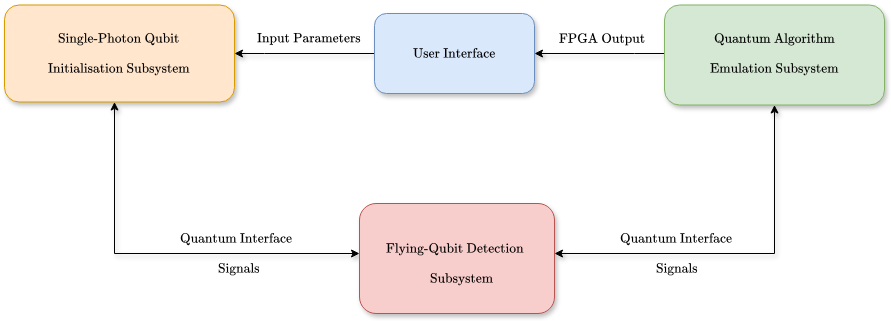
\includegraphics[width=\linewidth]{body/ch4/figs/overall-system-architecture}
	\caption[Subsystem Block Diagram.]{Overview system diagram showing the flow of data and instructions. A quantum computer is emulated on the FPGA belonging to the Quantum Algorithm Emulation subsystem.}
	\label{fig:overall-system-architecture}
\end{figure}

The figure also illustrates the proposed devices in the system, including an ARM-based microcontroller, FPGA, an electronic circuit for modelling the quantum interface, and a PC as part of the SPQIS and UIS modules. To compensate for differing operating frequencies, the proposed solution does not use a clock to synchronise the blocks. Instead, subsystems can communicate through \texttt{trigger} and \texttt{enable} signals to indicate the \texttt{start} and \texttt{end} of a process.

\subsubsection{Single-Photon Initialisation Subsystem}
The SPQIS initialises well-characterised qubits and defines the decoherence times of each qubit. To achieve this, the subsystem generates the probabilities of the quantum states of each qubit and interacts with the UIS to allow users to define the parameters that characterise the simulated quantum computer. Optimisation of the SPQIS involves considerations of accurate qubit representations, memory usage, and suitable preparation of qubits for transmission through the quantum channel in the FQDS. In turn, the manner in which qubits are prepared has an effect on the transmission rate of the quantum channel which can be measured as the number of flying qubits that are transmitted per second. The SPQIS is mainly facilitated on an ARM-based microcontroller. On the FPGA, the SPQIS manages the parameters of detected qubits through the circuit modelling the quantum channel. As shown in figure \ref{fig:overall-system-architecture} SPQIS is composed of:
\begin{itemize}
	\item 
	A pseudo-number generator for satisfying the initialisation of well-characterised, fiducial qubit quantum state	
	\item 
	Data structures and memory for storing qubit parameters
	\item 
	ARM-based microcontroller for initialising qubit
	\item 
	FPGA-based quantum computer emulator for initialising qubits as inputs to the quantum circuit or quantum algorithm performed
	\item 
	Electronic circuit that models flying qubits at the output
\end{itemize}
An overview of the SPQIS is illustrated in figure \ref{fig:spqis-overview} where a user prepares 3 physical qubit modelled in the quantum channel electronic circuit. Physical qubits are propagated through the quantum channel and detected by sensors in the FQDS module facilitated by the FPGA quantum computer emulator. 
\begin{figure}[!ht]
	\centering
	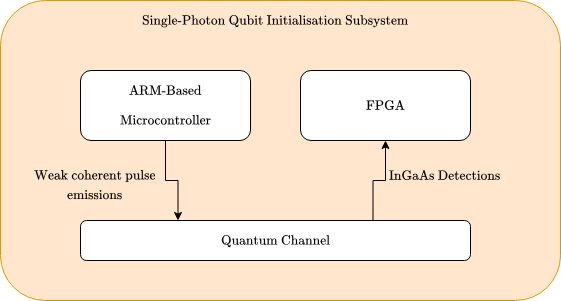
\includegraphics[width=\linewidth]{body/ch4/figs/spqis-overview}
	\caption[Single-Photon Qubit Initialisation Subsystem (SPQIS) Overview.]{The proposed design models the initialisation and transmission of single-photon qubits. Qubits are initialised on the microcontroller and mapped to physical qubits which are transmitted through the quantum channel. These "flying qubits" are decoded by the FPGA subsystem.}
	\label{fig:spqis-overview}
\end{figure}

The performance of this subsystem can be assessed from the  transmission rate and the power consumption. 

\subsubsection{Flying Qubit Detection Subsystem}

The aim of this module to model the detection of physical qubits through a quantum channel facilitated by a quantum network in which lasers are used to initialise and manipulate qubits. The main component in the subsystem is the electronic circuit that performs the quantum communication protocols for transmitting qubits between classical systems and a quantum computer. As noted in the literature, the apparatus of a quantum interface must have the ability to inter-convert stationary and flying qubits. Furthermore, the quantum interface should have the ability to transmit flying qubits between the sender's and receiver's private spaces \cite{divincenzo2000physical}. 

To fulfil this requirement, the proposed solution models photodetectors that convert flying qubits into stationary qubits. Flying qubits are propagated through the quantum channel modelling a fibre optic cable as illustrated in \ref{fig:fqds-overview}. 
\begin{figure}[!ht]
	\centering
	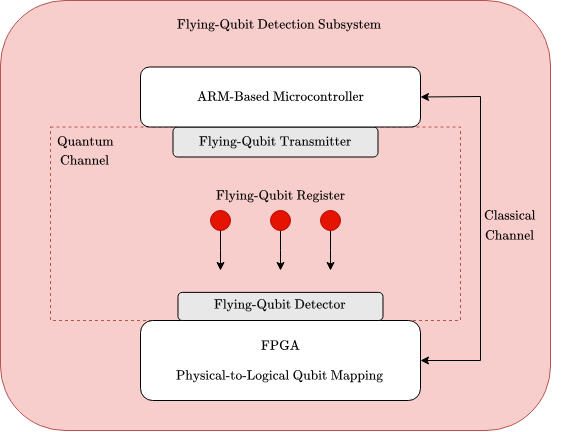
\includegraphics[width=0.85\linewidth]{body/ch4/figs/fqds-overview}
	\caption[Flying-Qubit Detection (FQDS) Subsystem Overview.]{Physical qubits are transmitted through the quantum channel in the FQDS module which enables physical qubits to be mapped to logical qubits on the FPGA system. The flying-qubit transmitter (CW laser) is modelled using LEDs, while the flying-qubit detector is modelled in a series of photoresistors or LDRs.}
	\label{fig:fqds-overview}
\end{figure}

The output from the photodetectors is transferred to the FPGA which encodes the physical qubits to logical qubits that can be used to perform quantum algorithms. The FQDS system consists of:
\begin{itemize}
	\item 
	A model of a fibre link that provides a secure path for the propagation of flying qubits
	\item 
	Electronic circuit with photodetectors for converting flying qubits to stationary physical qubits
	\item 
	FPGA for mapping physical qubits to logical qubits
\end{itemize}
The proposed solution models a bit-mapping gate by using the photodetectors to capture flying qubits in intervals, or detection windows. The number of qubits detected by the sensors needs to match the number of qubits transmitted from the SPQIS. Therefore, the performance of the FQDS is characterised by the decoherence times of the flying qubits, as well as the qubit detection rate. Consequently, the ratio between the qubit transmission rate and qubit detection rate is used to define the efficiency of the quantum channel. 

\subsubsection{Quantum Algorithm Emulator Subsystem}

To successfully implement quantum algorithms, the QAES defines a universal set of quantum gates and quantum circuits that describe the sequence operations on the qubits at the output of the FQDS. Since the QAES system is FPGA based, a high-level design and verification development workflow is proposed. Then, quantum gate operations are mapped to FPGA logic. Thereafter, the system is verified using RTL simulations before synthesising each block. Since quantum gate operations require manipulation of dense matrices which can lead to storage overheads, the memory schemes proposed aim exploit the capabilities of the FPGA by using a combination of distributed RAM and FIFO shift registers for storing quantum state information. The QAES system components include:
\begin{itemize}
	\item 
	A set of universal quantum gates
	\item 
	Quantum circuits for executing quantum algorithms
	\item 
	HDL code for synthesising quantum algorithms to the system architecture
	\item 
	FPGA hardware for emulating a quantum computer with onboard logic cells, DSP blocks and various IP cores
	\item 
	External memory for storing quantum state information and extending the storage capabilities of the FPGA	
\end{itemize}
The QAES system takes the output of the FQDS module and performs a quantum algorithm based on the user parameters defined in the SPQIS through the UIS module. The subsystem communicates with the ARM-based microcontroller to synchronise communication through the quantum channel. The output of the emulated quantum computer is a classical binary code that is returned to the UIS at the end of an algorithm. The UIS also allows users to select the quantum circuit or quantum algorithm to be performed by the QAES on the FPGA. 

Figure \ref{fig:fpga-design-flow} illustrates the design flow of the FPGA. The process begins with creating the register-transfer level (RTL) to match the functionality of the quantum algorithm to the hardware logic while operating on a data stream of qubits. 
\begin{figure}[!ht]
	\centering
	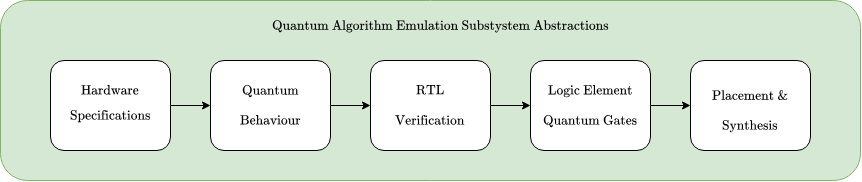
\includegraphics[width=1.0\linewidth]{body/ch4/figs/fpga-design-flow}
	\caption[Design Abstraction of FPGA-Based Quantum Computer Emulator.]{Due to the limited information in the system requirements, a top-down approach is adopted in order to add function details to the FPGA quantum emulator.}
	\label{fig:fpga-design-flow}
\end{figure}

The verification step ensures that the design works for the intended hardware architecture through appropriate testbench implementations. In the synthesis step, software development tools are used to transform RTL code representing quantum gate operations to digital logic gates and attempts to meet the register-to-register clock frequency while minimising resource usage on the FPGA. The FPGA system is integrated to the overall system, followed by implementation which produces a bitstream that is loaded to the device for FPGA programming. Finally, the QAES is lab tested and debugged using test inputs.

The performance of the FPGA when executing quantum algorithms is compared to the performance of PC-based quantum computer simulators. Furthermore, resource usage is compared to previous implementations of emulated quantum computers on FPGAs. Since power consumption depends on the register-to-register clock frequency and resource usage, the aim of the design is to minimise power consumption by reducing the number of resources required while performing quantum algorithms quickly.

\subsubsection{User Interface Subsystem}

Outputs from the FPGA-based QAES module are displayed graphically using PC-based software and a 7-segment display. The primary objective of the UIS module is to allow users to calibrate the system to run the desired algorithm on the system. Given that quantum algorithms require different qubit preparation techniques and quantum gates, the system also needs to allow users to define the inputs and select the quantum circuit that is required for experimentations. In summary, the UIS module allows users to:
\begin{itemize}
	\item 
	Define the initial qubit states
	\item 
	Select and configure the quantum circuit
	\item 
	Visualise outputs to help users understand the results from the quantum computer
\end{itemize}
The UIS interacts with the SPQIS to allow users to modify qubit preparation parameters before transmission through the quantum channel. Lastly, this subsystem allows users to upload results from the random number generator to the QAES system on the FPGA. 

\subsection{FPGA Resources for Modelling Quantum States \label{subsec:req-sim-qubits}}

For a quantum computer to exist, the qubits in the system need to satisfy the five criterion proposed by DiVincenzo \cite{divincenzo2000physical}. The method used to model qubits directly affects all the  system requirements. The first criterion that the simulated qubits must satisfy in order to accurately model the operation of quantum computing systems is that each quantum state needs to be well-characterised. As noted in the theoretical framework, the polarisation state, $\ket{\psi}$, of a photon, can be represented as a linear combination of the state vectors $\ket{\uparrow}$ and $\ket{\rightarrow}$, with coefficients $\alpha$ and $\beta$ that satisfy the normalisation condition in equation \ref{eqn:normalisation-condition}. Alternatively, qubits can represent the spin-state of atoms and fermions such as electrons. The polarisation states or electron spin-states are mapped to the computational basis set ${\ket{0}, \ket{1}}$. Therefore, in the computational basis, simulated qubit $\ket{\psi}$ should satisfy
\begin{align}\label{eqn:qstate-comp-basis}
	\ket{\psi}	& = \alpha_0\ket{0} + \alpha_1\ket{1}\nonumber\\
	\ket{0} = \left(\begin{matrix}
		1 \\ 0
	\end{matrix}\right)&~~;~~\ket{1} = \left(\begin{matrix}
	0 \\ 1
\end{matrix}\right)\nonumber\\
\ket{\psi} & = \left(\begin{matrix}
	\alpha_0\\
	\alpha_1
\end{matrix}\right)
\end{align}
where the coefficients $\alpha$ represent the wave amplitudes of the quantum state $\ket{\psi}$ that adhere to the normalisation condition derived from the Born postulate of quantum mechanics requiring that
\begin{align}
	|\alpha_0|^2 + |\alpha_1|^2 = 1\nonumber
\end{align}
Since classical bits cannot directly simulate the superposition of quantum states, the above representation of qubits requires more than one bit to store values of the amplitudes and vectors on a classical computer. Therefore, simulating a quantum computer requires the magnitudes of the basis states to be stored in order to model a well-characterised qubit. 

For this design, it can be assumed that if the system has $n$ qubits, then it can represent integer decimal numbers from 0 to $2^n-1$ which can be encoded in the computational basis as a string of bits to represent a multi-qubit state. For instance, a 4-qubit quantum computer is able to represent integers from 0 to 15, whereas a $3$-qubit quantum computer can represent integers from 0 to 7. Therefore, the performance, power consumption and memory usage of the system was expected to increase as the number of qubits $n$ increased. 

In general, the array structure of FPGAs consists of slices which comprise one or more programmable logic blocks; a routing network for interconnecting logic resources; I/O logic to communicate with the outside world; clock managers and hard-macros. The QAES exploits the structure of a FPGA to store and manipulate classical bits that represent quantum information. The methodology explores the application of Xilinx 7-series FPGA architecture in emulating quantum systems. In particular, LUTs and flip-flops can be used for memory as well as sequential and combinatorial logic. The proposed design aims to implement the $n$-input LUTs as both an asynchronous ROM and for performing $n$-input logic functions for quantum gate operations. Figure \ref{fig:amd-lut6} depicts the LUT6s which have 6-bit addressing to construct a 64-bit ROM \cite{amd2024support}. If a LUT6 is used to construct linear mappings between classical bits and the computational basis states, a single table can represent quantum registers with values from $\ket{0}_{10}$ up to $\ket{63}_{10}$ as seen illustrated in the figure. 
\begin{figure}[!ht]
	\centering
	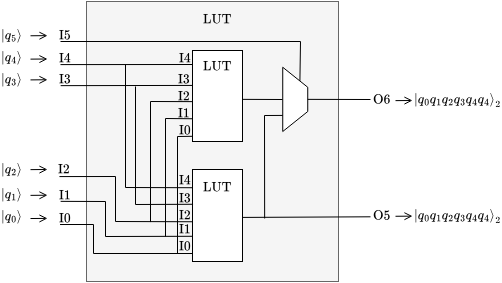
\includegraphics[width=0.85\linewidth]{body/ch4/figs/amd-lut6}
	\caption[Direct Mapping of Computational Basis States to Xilinx FPGA LUTs.]{Illustrating the proposed application of Xilinx 7-series LUTs for directly representing quantum registers for values between $\ket{0}_{10}$ and $\ket{63}_{10}$. The MSB corresponding to I0 is mapped to the qubit $\ket{q_0}$. Similarly, the LSB I5 is mapped to the qubit $\ket{q_5}$ in the quantum register. The output of the LUT represents the pure quantum register with a probability of 1.}
	\label{fig:amd-lut6}
\end{figure}

Each qubit in the quantum register representing a decimal number is associated with an \texttt{INIT} attribute of the FPGA LUT primitive consisting of a 64-bit hexadecimal value. Similar to real qubits, LUTs are initialised to a default value of zero, which implies that at if the inputs of a LUT6 are not specified, then the corresponding initial quantum state register is $\ket{000000}_2$. The  In other words, quantum states are generated from the binary encoding of some integer $\psi_{2}$ as a bit string $(q_0 q_1 \cdots q_{n-1})_2$. For example, when emulating a $6$-qubit quantum register using 6-input LUTs, the integers $\psi_1 = 3_{10}$ and $\psi_2 = 5_{10}$ can be represented in the computational basis as 
\begin{align}
	\ket{\psi}_{2}	& = \ket{q_0 q_1 q_2 \cdots q_{n-1}}_2\nonumber\\
\implies~~	\ket{\psi_1} = \ket{3}_{10} & = \ket{000011}_2 \nonumber\\
	\ket{\psi_2} = \ket{5}_{10}	& = \ket{000101}_2\nonumber
\end{align} 
As noted in the theoretical section, such a multi-qubit system combines the Hilbert spaces of each quantum state as the tensor product
\begin{align}
	\ket{000011}_2	& = \ket{0}\otimes\ket{0}\otimes\ket{0}\otimes\ket{0}\otimes\ket{1}\otimes\ket{1}\nonumber\\
				& = \left(\begin{matrix}
					1\\
					0
				\end{matrix}\right)\otimes\left(\begin{matrix}
				1\\
				0
			\end{matrix}\right)\otimes\cdots\otimes
			\left(\begin{matrix}
				0\\1
			\end{matrix}\right)\otimes
		\left(\begin{matrix}
			0\\1
		\end{matrix}
		\right)\nonumber\\
		& = (0,0,0,1,0,0, ..., 0)^T\nonumber
\end{align}
For the integer $5_{10}$, the equivalent 6-qubit quantum register can be represented as the column vector given by
\begin{align}
	\ket{000101}_2	& = (0,0,0,0,0,1,...,0)^T\nonumber
\end{align}
These examples illustrates that the position of 1 in the column vector corresponds to the value of the number in the computational basis, i.e. when the integer number is $d$, then the position of 1 in the column vector is $d + 1$. This example also illustrates that in the computational basis, to simulate a relatively small integer in a 6-qubit quantum system could require substantial power, memory and resources, such as LUTs and DSP slices. The size of these column vectors grows exponentially with the number $n$ of qubits, as noted previously. For example, to represent the integer 3 in the computational basis of a 12-qubit quantum computer would require double the amount of memory to store the number. In general, a $n$-qubit produces quantum registers that can be represented as a column vector with $2^n$ entries. This has a direct effect on the fulfilment of system requirement NRF04 which states that resource usage, memory and computational overhead should be minimised. Overall, number of LUTs used in the hardware was expected to increase with the number of qubits in system.

\subsection{Emulation Accuracy in Relation to Quantum State Amplitudes}

In addition to the considerations made on the increase in memory and resource requirements as the number of qubits is increased, an inspection of the amplitude coefficients is critical in design the quantum computer emulator. As noted in equation \ref{eqn:multiple-qubit-state}, a 3-qubit wide quantum register representing an integer $\psi$ is in a state of superposition given by
\begin{align}
	\ket{\psi} & = \alpha_0 \ket{000}_2  + \alpha_1 \ket{001} + \alpha_2 \ket{010} + \alpha_3 \ket{011}\nonumber\\& + \alpha_4 \ket{100} + \alpha_5 \ket{101} + \alpha_6 \ket{110} + \alpha_7 \ket{111}\nonumber 
\end{align}
where each $\alpha_{i}$ is a complex probability that satisfies
\begin{align}
	\sum_{i=0}^{7}|\alpha_{i}|^{2} =  1\nonumber
\end{align} 
Since each $\alpha_{i}$ is a complex number, entries in the column vector of the quantum register that are equal to 1 would need to be replaced by two values. Furthermore, the normalisation constraint on the $\alpha_{i}$ coefficients implies that the magnitude of these complex coefficients must add up to 1, i.e. $0 \leq \alpha_{i} < 1$. The accuracy of the quantum emulator in appropriately modelling a quantum computer depends on the resolution of the number scheme chosen as well as the hardware platform on which an experiment is performed. 

For a PC-based compiler, the precision of the number depends on the resolution of the floating-point number in the $\texttt{float}$ data type. The $\texttt{double}$ data type can also store the amplitudes of the coefficients as a 64-bit number. However, floating-point data types on microcontrollers tend to produce code which uses a substantial storage space. The code is generally also slow because of the complexity of simulating floating-point operations. If the numbers were to be stored in complex form, each entry in the quantum state column vector that is non-zero would need two numbers to store information about the qubit in memory. Furthermore, the design needs to be able to handle potential overflow conditions due to multiplication or division operations. Therefore, the representation and storage of the complex coefficients directly affects system requirements FR03, FR05, FR06 and NFR04, in relation to the FPGA and PC interface, data transfer and processing, correctness and resource efficiency.

On a FPGA, a floating-point number can exist as a fixed number of significant digits and scaled using an exponent in some fixed base. FPGAs typically support \texttt{half}, \texttt{single}, and \texttt{double} format types for representing floating-point numbers. The floating-point encoding scheme is maintained by the IEEE/ANSI 754-1985 standard where a basic number utilises an 8-bit exponent and a 24-bit mantissa as illustrated in figure \ref{fig:floating-point}. The standard fixed-point scheme can represent an unsigned number between 0.0 and 255.9906375 or a signed number between -128.9906375 and 127.9906375 using two's complement. The proposed design stores probabilities with four significant numbers, for example, an amplitude of $1/\sqrt{8}$ is stored as 0.3536. 

For quantum state probabilities represented as signed numbers, the range of values that can be presented also depends on the encoding scheme that is used in the method. It is noted however, that the decimal or part of the probabilities of the quantum states is always 0 or 1, thus, the emulation accuracy would mostly depend on the number of mantissa or fractional bits used. 
\begin{figure}[!ht]
	\centering
	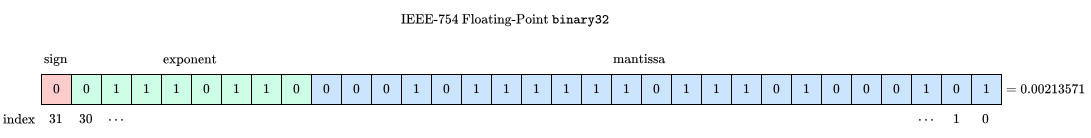
\includegraphics[width=\linewidth]{body/ch4/figs/floating-point}
	\caption[Illustrating the IEEE 754-1985 Standard for 32-bit Floating-Point Numbers.]{The IEEE 754 standard gives precision of 6 to 9 significant decimal digit precision by employing a sign-bit, 8 exponent bits, and 24 mantissa bits with 23 bits that are stored explicitly.}
	\label{fig:floating-point}
\end{figure}
Alternatively, fixed-point numbers use fixed binary point instead of a floating decimal point with a dynamic location based on the value of the exponent. An implied binary point separates a binary number into $u$ integer bits and $v$ fractional bits as illustrated in figure \ref{fig:fixed-point}.
\begin{figure}[!ht]
	\centering
	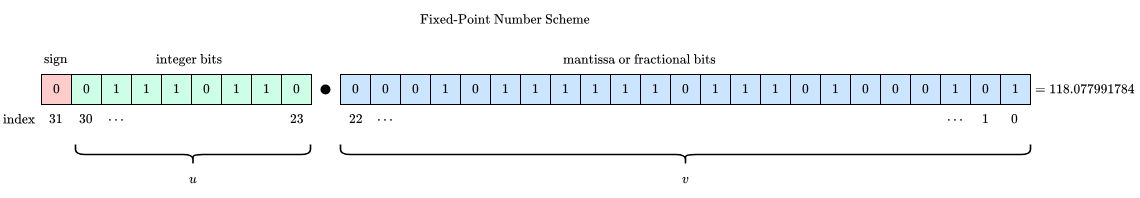
\includegraphics[width=\linewidth]{body/ch4/figs/fixed-point}
	\caption[Illustrating a 32-bit Fixed-Point Scheme.]{A 16-bit fixed point number with $u$ integer bits and $v$ fractional bits. The choice of $u$ and $v$ has a direct effect on the performance and power efficiency of the FPGA.}
	\label{fig:fixed-point}
\end{figure}
The choice of $u$ and $v$ directly affects the range and precision of the number presented, in relation to correctness and emulation accuracy of the FPGA. A trade-off has to be made in terms of the size of the number presented and the accuracy of the representation. For example, in a Q15.16 format, there are 16 bits for representing the integer and 16 bits for representing the integer part, making a total of 32-bits. Increasing the number of integer bits would increase the range of whole numbers that can be represented. In contrast, more fractional bits could improve the precision by allowing for granularity in representing the amplitudes of the quantum states. Reducing the number of fractional bits could reduce the accuracy of the quantum emulator. 

Proper scaling of the integer and fractional bit-widths involves moving position of the binary point to ensure that numbers fit within the possible range while maintaining precision \cite{harvie2024how}. If scaling is not done correctly, fixed-point arithmetic operations could lead to bit overflow errors. This can be prevented using techniques such as saturation arithmetic which limits representable values to a maximum and minimum value. Alternatively, numbers that require a larger bit-width can be indirectly represented using modular arithmetic which wraps values around the maximum and minimum representable numbers in the scheme. In addition to overflow errors in the fixed-point scheme, quantisation errors were expected to have a direct effect on the accuracy of the quantum computer emulator. Quantisation errors arise naturally from converting a floating-point number to a fixed-point number.

\subsection{Graphical Representations of Qubits}

Instead of storing the complex amplitudes directly as a real and imaginary values in the column vector, well-characterised qubits and quantum states can be represented graphically on the surface of a Bloch sphere or as vectors in a unit circle. For example, in the computational basis, the quantum register $\ket{011}$ can be represented as shown in figure \ref{fig:bloch-011}. 
\begin{figure}[!ht]
	\centering
	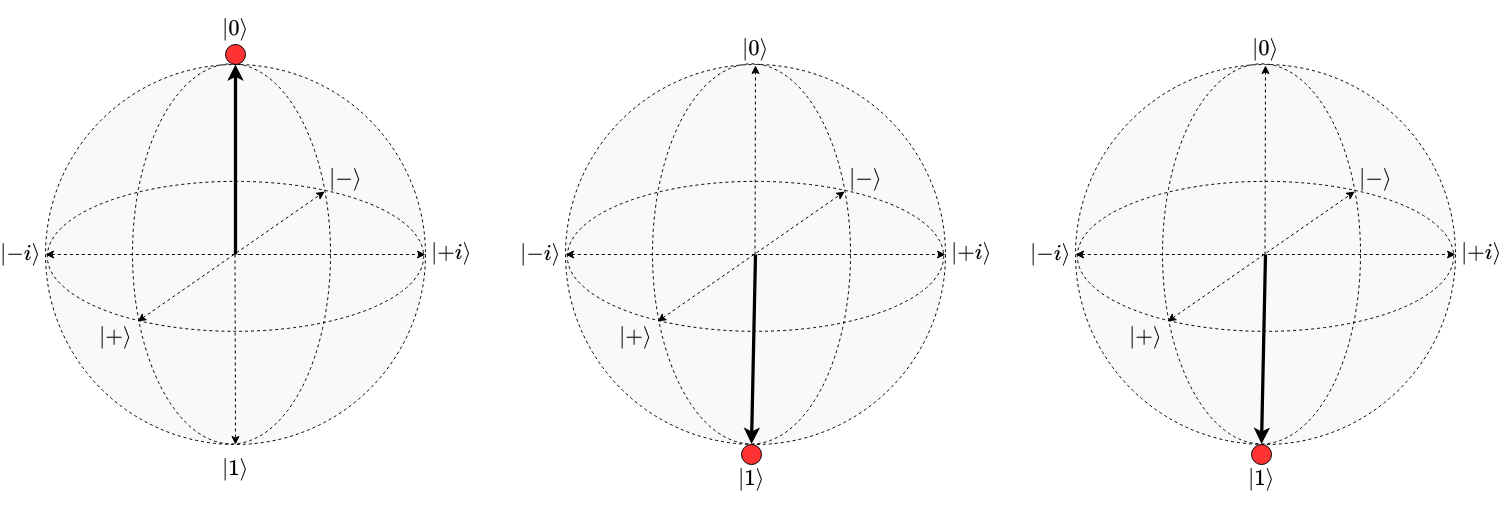
\includegraphics[width=0.94\linewidth]{body/ch4/figs/bloch-011}
	\caption[Bloch Sphere Representation of the Integer 3.]{A 3-qubit quantum state register can be represented on the surface of a Bloch sphere in the computational basis.}
	\label{fig:bloch-011}
\end{figure}
A unit circle, similar to the one implemented by Hlukhov, can be used to encode the positions of the unit vector based on the phase $\theta$ of a qubit as shown in figure \ref{fig:unit-circle}. 
\begin{figure}[!ht]
	\centering
	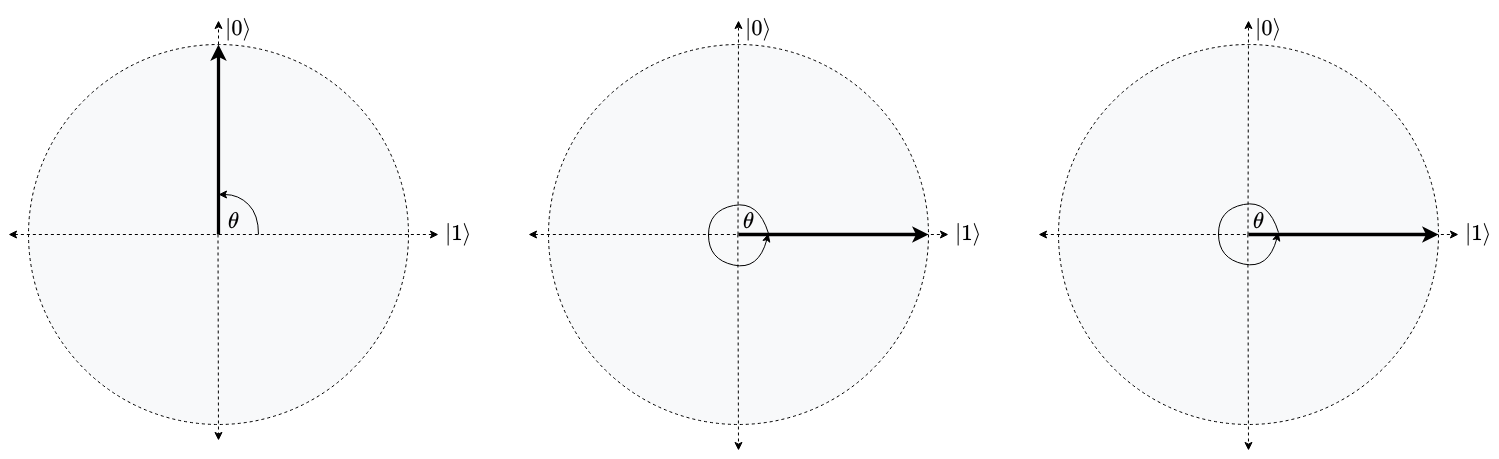
\includegraphics[width=0.94\linewidth]{body/ch4/figs/unit-circle-011}
	\caption[Unit Circle Graphical Representation of Integer 3.]{The 3-qubit register can be represented graphically on a unit circle. The phase $\theta$ of the quantum states can be used to minimise resource usage and memory.}
	\label{fig:unit-circle-011}
\end{figure}
Both representation afford the opportunity to represent the quantum state of qubits with respect to a single value corresponding to the phase $\theta$. Using the complex representation would require four values to represent one quantum state amplitude. However, noted in theoretical framework is that the normalised amplitudes can be expressed as the sinusoidal functions
\begin{align}\label{eqn:amplitude-sinusoids}
	\alpha_0	& = \sin(\theta)\\
	\alpha_1    & = \cos(\theta)
\end{align}
to produce the unit circle representation. The difference between the two graphical representations considered in the proposed design is that the Bloch sphere representation also requires storage of the relative phase of the qubit. This representation allows for more complex qubit operations that are not necessarily realisable on physical quantum computers. Furthermore, the spherical and circular representations can be used to display information about quantum states in a more intuitive manner to the user. 

\subsection{Methods for Initialising Qubits and Transmitting Quantum Information through a Quantum Channel \label{subsec:req-sim-gates}}

Satisfying the requirement for initialising qubits to a simple fiducial state is also considered from the perspective of the quantum interface. The model also considers qubit coupling to satisfy DiVincenzo's criteria. Users need to be able to initialise both physical and logical bits in the system.

In the proposed model, initialisation and transmission of well-characterised qubits is simulated using light from 8 GaAs LEDs to model Kimble et al. and Li et al.'s techniques for fabricating and capturing single-photon qubits using lasers, atoms and quantum dots \cite{turchette1995measurement, li2022control}. Physical qubits are coupled to one another using a collinear processor mapping in which the first qubit is coupled to the second qubit and the second qubit is coupled to both the third and fourth qubit. For the purposes of this design, the collinear mapping has no effect on the final result. Moreover, the system uses similar techniques to those employed in the QKD systems, such as the COW and Ent QKD systems, where a sender, Alice, transmits data to a receiver, Bob, through a quantum channel that exploit quantum entanglement. At the receiver of the quantum channel, InGaAs quantum dots and avalanche photodiode detectors are modelled using photoresistors in a BJT-based switching circuit. 

Preparation of qubits at Alice's location is modelled on the ARM-based microcontroller which toggles the LEDs to simulate propagation of flying qubits of weak coherent states from a CW laser as implemented in by the SECOQC project. Logical qubits in the proposed design are prepared in the computational basis and mapped to the physical qubits modelled by the LEDs, before transmission through the quantum channel. This is done through the linear qubit physical-to-logical qubit mapping scheme that is defined intrinsically on both the microcontroller and the FPGA in the SPQIS and QAES modules. For example, when an LED is \texttt{ON}, this could represent the $\ket{1}$ quantum state, while a LED that is \texttt{OFF} could represent the $\ket{0}$ states. Alternatively, a LED \texttt{ON} in a transmitted sequence could represent the position of 1 in the Hilbert space of the system as shown below. In both cases, probabilities can be preloaded to the devices from a pseudo-random number generator with a uniform distribution. 

\subsubsection{Quantum Channel Transmission Mode 1: Flying-Qubits in Binary Encoded Quantum Registers}

In the first method, each LED sequence represents a quantum register given by $\ket{q_{0}q_1\cdots q_{n-1}q_n}$. This method is illustrated in figure \ref{fig:qubit-mapping-method-1} where the quantum register $\ket{00010000}$ is directly reflected in the LED pattern in the sequence. Mathematically, this method for modelling qubit transmission through the quantum channel transfers the tensor product 
\begin{align}
	\ket{00010000}	 &  = \ket{0} \otimes \ket{0} \otimes \ket{0} \otimes \ket{1}\nonumber\\& \otimes \ket{0} \otimes \ket{0} \otimes \ket{0} \otimes \ket{0}\nonumber
\end{align} 
through a 1-1 mapping between quantum state $\ket{q_i}$ and LED $q_i$ in the sequence.
\begin{figure}[!ht]
	\centering
	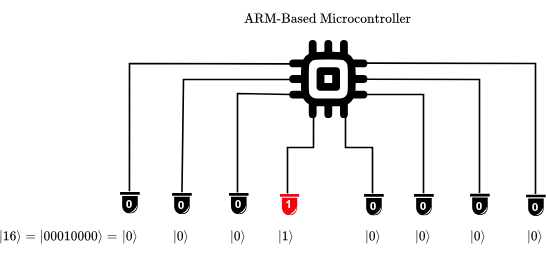
\includegraphics[width=\linewidth]{body/ch4/figs/qubit-mapping-method-1}
	\caption[Qubit Mapping Using LEDs for Direct Representation of the Computational Basis States $\ket{0}$ and $\ket{1}$.]{Illustrating the first method for initialising and transmitting quantum states directly as the tensor product $\ket{q_0} \otimes \ket{q_1} \otimes \cdots \ket{q_{n-1}}$. In this method, a single LED flash represents the basis vector $\ket{1}$ and a dim or \texttt{OFF} LED represents $\ket{1}$.}
	\label{fig:qubit-mapping-method-1}
\end{figure}
Using this direct qubit mapping technique provides a more straightforward way of modelling quantum computers with $n = 8$ qubits. For simulations of systems with less than 8 qubits, $n < 8$, the system must be able to discard or ignore parts of a transmitted LED sequence. For example, to represent a quantum system where $n = 3$, the only 3 LED out of 8 are required to transmit qubits in the quantum channel. Systems with $n > 8$ require multiple sequences to in order to transmit a full register. For example, to simulate the transmission of a system with $n = 12$ qubits, this method would require two and a half sequences to transmit the full register. In general, the number of sequences $s_1$, required to model an $n$-qubit transmission is given by
\begin{align}\label{eqn:number-of-sequences}
	s_1 & = n\cdot 2^{-3}
\end{align}
If $n$ is not a multiple of $2^3$, then the remainder from the division represents the portion of the LED sequence that can be discarded at the receiver. When a user initialises the system and sets input parameters related to the number of qubits, the system is should define the total number of LED sequences and the information that can be disregarded in the communication. 

This method was expected to provide a lower communication throughput and higher qubit transfer rates than the methods described below. In addition, given a system with $n$ bits, this method can transmit all the information about a quantum state using fewer LED sequences. Therefore, this method was expected to require less power than the other methods. From this analysis, it can be seen that power and the number of repetitions can be suitably employed as metrics for measuring the performance and communication efficiency of the quantum interface. 

\subsubsection{Quantum Channel Transmission Mode 2: Communicating with Quantum State Hilbert Spaces}
The second qubit initialisation and transmission technique also allows for a direct representation of qubit couplings as the quantum channel essentially transmits the topology of the Hilbert space of the quantum state in a pure form. This is because the 8 LED \texttt{ON} and \texttt{OFF} states can be directly mapped to the entries of the state column vector of a 3-qubit quantum register. For example, the column vector shown above for the computational basis representation of the integer 3 can be modelled using 8 LED bits as demonstrated in figure \ref{fig:led-qubit-mapping}. \\ 
\begin{figure}[!ht]
	\centering
	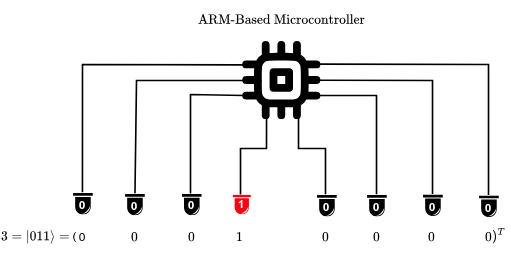
\includegraphics[width=1.0\linewidth]{body/ch4/figs/qubit-mapping-leds}
	\caption[Qubit Mapping Using LEDs to Represent 0s and 1s in Quantum State Vectors in the Computational Basis.]{A demonstration of a possible qubit mapping using the 8 LEDs to represent the 0s and 1s in the quantum state column vector that represents the integer $3_{10}$ in the computational basis as $\ket{011}_2$. The illustration shows \texttt{OFF} LEDs (0) in black, while the red colour illustrates an LED in the \texttt{ON} state. Note that, although the LED sequence is identical to the one shown in \ref{fig:qubit-mapping-method-1}, the information that is represented is not the same.}
	\label{fig:led-qubit-mapping}
\end{figure}
This method allows the quantum state to be transmitted as a vector through the quantum channel, offering a direct model of the quantum states that propagates through quantum channels as single-photons. To represent quantum computers with $n > 3$ qubits, multiple \texttt{ON} and \texttt{OFF} sequences can be programmed to ensure that all the $2^n$ matrices are displayed. Since each sequence can represent up to $8$ entries of the basis column vector, a factor of $2^3$ can be extracted from the $2^n$ entries to show that the number of LED sequences, $s$, that need to be performed to fully represent a quantum system with $n>3$ qubits is given by
\begin{align}\label{eqn:led-repetitions}
	s_2 & = 2^{n-3}
\end{align}
As a further illustration, consider the case where a 5-qubit quantum computer is being modelled. In this instance, the 8 LEDs have to flash 4 times in order to represent the basis column vector fully. This implies that the increasing the number of qubits in the system also increases the communication complexity and the throughput of the emulated system. Moreover, entangle qubits present a larger communication overhead in the quantum channel. This is due to the fact that entangled states come in EPR pairs, which require double the resources to represent each state of the pair. If qubits are entangle, Alice and Bob are required to share halves of the EPR states at the start of the communication protocol.

According to literature, these quantum states need to have sufficiently long enough decoherence times. For the proposed design, decoherence times of qubits is correlated to the duration of the \texttt{ON} and \texttt{OFF} LED pulses. Different pulse durations can be tested to simulate the effect of different decoherence times on the throughput and latency of a quantum communication system that is facilitated in the interface between a quantum computer and a classical computer. The communication protocol that handles the transfer of the bits requires a clear separation between signed, integer bits and mantissa bits. Since the modelled CW laser has large coherence times, the clocks on both the microcontroller and FPGA board can be used independently to control the emission and detection of simulated single-photon qubits. Tests can be conducted to find the optimal simulation of the decoherence of qubits based on the clock frequencies of the different boards. In an implementation of a quantum channel in a QKD network at the SECOQC project, TREL used a one-way weak pulse system that transmits optical pulses at a repetition rate of about $\SI{7}{\mega\hertz}$. In contrast, available microcontroller and FPGA clocks can operate at frequencies between or over $\SI{48}{\mega\hertz}$ to $\SI{133}{\mega\hertz}$, which is sufficient to model the operation of a quantum channel a the QKD network. 

LED sequences can be driven by the GPIO pins of the microcontroller. LED pulse sequences, whether representing the a 0s and 1s in the column vector or the phase, must be synchronised on the same clock to ensure that the LDR sensors on FPGA detect the pulse sequences in the correct window to avoid ambiguity in the quantum states. User need a way to initialise the qubits at the same time. Notably, the ARM-based model of the CW laser controller is not required to perform any computations. Quantum algorithms and quantum gate operations are performed on the FPGA only. To ensure security in models of quantum teleportation and key distribution, qubit paths in the quantum channel are occluded inside a tubular cases as illustrated in figure \ref{fig:led-to-ldr}, where each LED is directly aligned to the detection system connected to the FPGA such that one LDR can detect light from 1 LED.
\begin{figure}[!ht]
	\centering
	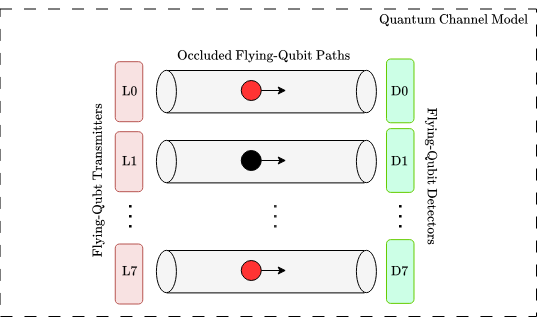
\includegraphics[width=1.0\linewidth]{body/ch4/figs/led-to-ldr}
	\caption[Illustration of the Security Measurements Implemented in the Quantum Communication Channel.]{An illustration of the occluding flying-qubits in order to prevent attacks from an eavesdrop. Moreover, in line with physical quantum computers, the user has no direct access to qubits in the entire emulated system except during initialisation and when performing measurements on the output.}
	\label{fig:led-to-ldr}
\end{figure}

When a measurement is performed on a qubit, it collapses to a classical bit according to the probabilities. This implies that the outputs from the FPGA quantum emulator should be able to represent qubits and classical bits on quantum and classical channels, respectively. Information about quantum state, for example, phase or probabilities, must be consistent on both platforms. Since the LEDs only represent the basis states, the communication protocol needs to include method of associating a probability or angle to each qubit. In this proposal, probabilities can be generated from a uniform distribution in MATLAB prior to starting the system. The generated probabilities can be preloaded on the microcontroller or stored in external memory on the FPGA.

\subsection{Flying Qubit Detection and Synchronisation of Classical and Quantum Systems \label{subsec:fqds-synch-requirements}}

The light from the LEDs propagates through the quantum channel through a model of a fibre link as implemented in the QKD systems explored in literature. Since the proposed design is for research purposes and modelling the operation of a quantum computer in laboratory settings, the short length of the modelled fibre link was not expected to contribute significantly to flying-qubit propagation delays. The design uses a series of 8 photoresistors, or LDRs, to simulate the use of single-photon InGaAs APD sensors for capturing flying qubits in the computational basis while ensuring that the quantum channel is secure. 

APDs are more sensitive devices that are used in specialised cases, whereas photoresistors are typically used as low cost photo sensitive elements. The aim of the photoresistor circuit is not to model the physical properties of APDs. Instead, the photoresistor circuit aims to model transmission of quantum information in the form of light. Due to their low-cost and sensitivity to light, photoresistors are suitable for modelling the conversion of quantum information from flying qubits to stationary qubits. 

In the proposed design, modelled flying-qubits are transmitted and recaptured within a detection window. If an LED is \texttt{ON} in the window, the resistance of the photosensors decreases, corresponding to the qubit state $\ket{1}$. If an LED is \texttt{OFF}, the resistance increases, corresponding to the state $\ket{0}$. Since the high resistance state corresponds to the $\ket{0}$, qubits are initialised in appropriately in the ground state on the quantum computer emulator. Photoresistors typically take time to transition between the high and low resistance states. This transition time between high and low resistance states was expected to contribute to communication delays, thereby affecting the overall communication efficiency of the model of the quantum channel. 

Furthermore, the transition time between resistance states directly affects the duration of the detection window. If the transmission time of the sensors is $t_s$, then the \texttt{ON} and \texttt{OFF} times of the LEDs, $\tau$, should be greater than $t_s$. To compensate for other errors and delays, an additional time $t_\epsilon$, is added to the on-and-off time to ensure that the total duration of the detection window is sufficiently long enough to capture data. By adjusting the on-and-off times, errors can be introduced into the system for perform quantum error correction experiments. 

To ensure that the detection window is initialised at the same time on the ARM microcontroller and the Xilinx FPGA, the proposed solution uses a \texttt{trigger} signal in a configurable bus as illustrated in figure \ref{fig:trigger}. The same line is used to allow the user to \texttt{enable} and \texttt{reset} the system in case they want to make changes to the input parameters. A different line, the \texttt{ack} signal, is used to allow the devices to communicate during the different stages of the communication protocol. The communication protocol depends on the format in which the qubits are transmitted through the quantum channel. If transmission mode 1 is used, then the first step in the communication protocol would require the source microcontroller to indicate to the FPGA emulator that the information is transmitted as pure quantum states. This can be accomplished by transmitting a 0 or 1 through the \texttt{async} line after the user has selected the qubit mapping at the source. 

\begin{figure}[!ht]
	\centering
	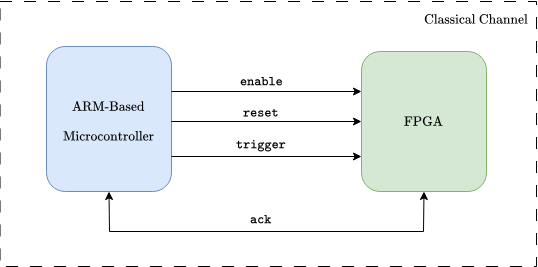
\includegraphics[width=1.0\linewidth]{body/ch4/figs/trigger}
	\caption[Illustrating the Classical Channel Between the ARM-Based Microcontroller and the FPGA.]{A \texttt{trigger}, \texttt{enable} and \texttt{reset} signal is transmitted through the bus between the microcontroller and FPGA. The \texttt{ack} signal is used at different stages of communication protocols to indicate when information has been transmitted.}
	\label{fig:trigger}
\end{figure}

Careful considerations were made in the design regarding minimum and maximum logic voltage levels and the maximum current that can be supported by the GPIO pins of the microcontroller and FPGA. To limit the collector current $I_C$ while maintaining the required voltage logic levels, the proposed electronic circuit for modelling qubit detection uses the photoresistors to divide the base voltage $V_B$ of a NPN type BJT. When the photoresistor is occluded, the BJT is in the cutoff region, and no current can flow. When light from the LEDs is incident on the photoresistors, the BJT is saturated and current can flow through the collector to the emitter. Therefore, current flows through the sensor when an LED indicates the quantum state $\ket{1}$. This feature of BJTs ensures that the resistance states, corresponding to the basis states, are well separated. Additionally, the maximum current through the BJT is determined by the gain. Therefore, the selection of the BJT depends on the current gain and the maximum current that is supported by the FPGA. 

Since flying qubits and their preparation are modelled using LEDs in the visible spectrum, an eavesdropper, Eve, can perform attacks simply by looking at the communication channel. Using a similar approach to the illumination-based method proposed by Lydersen et al. for preventing fake-attacks through background illumination of APDs, the proposed design uses an obscured quantum channel that prevents attackers from observing prepared quantum states or inducing false detections at the photosensors. By using an opaque fibre link, the model can securely transmit flying qubits from the source to the detectors. In addition, by covering the quantum channel, the model was expected to successfully transfer qubits with low transmission losses and a reduced false-detection rate from detection of lights in the environment. 

Overall, the electronic module modelling a quantum channel needs to be compatible with the peripherals on the FPGA board. FPGAs typically have female connectors for direct connection of peripheral module boards. Therefore, the quantum channel module is required to have male connectors. As mentioned, the output signal from the peripheral quantum channel module should conform to the LVCMOS 3.3V or LVTTL 3.3 logical conventions to improve resistance state detection precision \cite{diligent2011pmod}. On Xilinx FPGAs, the I/O pins generally have symmetrical $\SI{24}{\milli\ampere}$ source and sink capabilities \cite{diligent2011pmod}. In contrast, the drive strength of microcontrollers is generally less, typically in the range between $\pm\SI{5}{\milli\ampere}$ and $\pm\SI{10}{\milli\ampere}$) \cite{diligent2011pmod}. The proposed solutions uses the microcontroller to drive the emitter and receiver of the quantum channel model. The photoresistor circuit employs the Pmod Interface Type 1 interface for general purpose logic. Therefore, the GPIO pins on the microcontrollers should be configured as outputs while the Pmod GPIO pins on the FPGA should be set up as inputs. 

On the microcontroller, bit patterns on the LED circuit can be toggled using embedded C. On the FPGA, Verilog HDL code can suitab ... The use of appropriate delays is crucial for modelling the decoherence times of qubits and configuring the duration of a detection window. 

\subsection{Storing Qubits on the FPGA}

After a qubit is detected, the quantum state information needs to be stored on the FPGA according on the transmission method selected by the user at the start of an experiment. In the direct representation of qubits state, each qubit is detected and stored directly as a bit in memory in order to maintain the same sequence of qubits. This method allows for efficient retrieval and manipulation of qubits during emulation. The stored string of bits can be interpreted as the tensor product of the basis states. Each basis state can be store in the external memory of the FPGA along with the probabilities or phases associated with each state. 

At the end of the detection window, a digital signal is transmitted through the \texttt{ack} line from the microcontroller in the classical channel to the FPGA to indicate that transmission is complete. To further remove ambiguity in qubit states, the communication protocol transfers an additional bit through the \texttt{trigger} to enable the use of gray code for labelling the different properties of the qubit stream in a finite state machine. For example, if the \texttt{trigger} bit is zero and the states are not entangle, then the bit sequence 00 is transmitted to indicate to the emulated quantum computer that the qubit transfer is complete. If the quantum states are entangled, then the signal carrying 01 is transmitted to indicate that a Bell state measurement has been performed by Alice at the source.

Information about the quantum algorithm to be performed can also be encoded in the digital signals transferred through the classical net. Once the final \texttt{ack} signal is received, the FPGA can perform scalar multiplication of the state vectors with the preloaded probabilities. The output of the scalar product is stored in a different part of the FPGA memory to complete the initialisation of qubits on the emulated quantum computer. The total number of registers used in memory depends on the user defined parameters and the register widths depend on the number of mantissa bits in the fixed-point representation of phases and probabilities. 

The second quantum channel transmission mode which transfers the Hilbert space of a qubits was expected to require more registers to store quantum state data on the FPGA at the start of an experiment. For this method, the ground state Hilbert space of the $n$-qubit quantum register is preloaded in external memory along with the phases using a fixed-point representation. Similar to the previous method, the qubit stream is stored as a bit-string in the external memory of the FPGA. Once a signal indicating the end of a detection window is detected by the device, elements in the stored column vector of the ground state are updated with the correct amplitudes. 

Regardless of the transmission mode selected, software-based error detection mechanisms need to be enforced in the FPGA to check for inconsistencies in the received qubit states, particularly during quantum error correction experiments. The error detection mechanism needs to ensure that the stored qubits on the FPGA reflect the transmitted qubits accurately. Although more straightforward to implement, the first method was expected to require more clock cycles (and therefore more power) for storing the full description of a well-characterised qubit in memory since the quantum register is in the decomposed tensor product form. This is because the first method requires further processing before storing the complete column matrix of the qubit Hilbert space for further processing with quantum gate operations.

Most FPGAs offer various external memories, including DDR2 and DDR3 SDRAM as some of the common high-performance memory types for storing large amounts of data and enabling fast read and write operations through high-speed interfaces such as the advanced extensible interface (AXI4). Xilinx 7 series FPGAs use SLICEMs to implement function generators or LUTs as synchronous RAM registers called distributed RAM (DRAM) elements \cite{xilinx20167series}. DRAM modules provide asynchronous write capabilities and allow synchronous read operations to be implemented with a flip-flop in the same slice to improve the performance \cite{xilinx20167series}. 

RAM elements can be configured within a SLICEM to implement different combinations of ports and data widths. Using the single port configuration to perform storage operations on the quantum state representations could prove to be slow since synchronous writes and asynchronous reads are performed on the same address bus. More suitable distributed RAM configurations include the dual port, simple dual port and quad port configurations whose multiple ports can be used for synchronous writes and asynchronous reads of quantum state vectors. On the Xilinx 7 series FPGAs, maximum data transfer can be achieved using the quad port configuration which uses one port for synchronous writes and asynchronous reads, and three ports for asynchronous reads \cite{xilinx20167series}. In each case, all storage elements share in the distributed RAM share a common control signal clock (CLK), control enable (CE) and set/reset (SR). CE and SR signal are active high. To store quantum state information on the distributed RAM, storage elements can be forced into the state specified by the logic of the SR signal. 

To avoid using flip-flops which potentially requires more clock cycles for storing sensor data, SLICEM function generators can be configured as 32-bit shift registers such that each LUT can delay serial data from 1 to 32 clock cycles. Since the clocks rates of the FPGA and microcontroller are not the same, this method is more suitable since asynchronous FIFO I/O buffers can be used to facilitate read and write operations on the clock domain of the FPGA only. Using the first qubit transmission technique where the LED status indicates the computational basis state, photoresistor detection data can be stored in the FIFO as soon as they are detected. Since each detection is 8 bits, each clock cycle would store eight quantum states in a quarter of a 32-bit shift register on the FPGA. Figure \ref{fig:fifo-shift-register} illustrates the construction of a 32-bit shift register occupying a single LUT. Smaller shift registers can be built on Xilinx FPGAs by varying the address of LUT outputs corresponding to the desired width \cite{xilinx20167series}. For example, a 13 bit register can be configured by setting the address of the LUT output in the CLB slice to the 13th bit \cite{xilinx20167series}.
\begin{figure}[!ht]
	\centering
	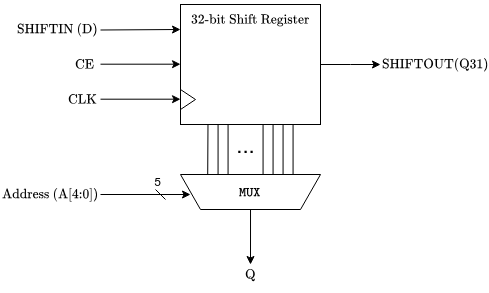
\includegraphics[width=0.85\linewidth]{body/ch4/figs/fifo-shift-register}
	\caption[Xilinx 7-Series 32-bit Shift Register.]{Xilinx 7-series FPGAs allow FIFOs to be implemented using the illustrated 32-bit shift register primitive. Write operations are synchoronous with the clock input (CLK) and the optional clock enable (CE). Shift registers are used to store sensor values in real-time. Shift registers allow dynamic reads through the LUT outputs labelled Q by varying the address \cite{xilinx20167series}. This feature is used later to specify the number of qubit quantum state vectors to be transferred to the distributed RAM.}
	\label{fig:fifo-shift-register}
\end{figure}

Using an asynchronous FIFO ensures that read and write operations of qubit detections can be written to the FIFO from the quantum channel circuit for different decoherence times. As the FIFO is read, qubit state vectors can be stored in distributed RAM elements. 

\subsection{Simulating Quantum Algorithms on a FPGA \label{subsec:req-sim-qualgorithms}}

The proposed design aims to emulate the following quantum algorithms and their associated quantum circuits:
\begin{enumerate}
	\item 
	Quantum Teleportation
	\item 
	Quantum Fourier Transform
	\item 
	Quantum Factoring Algorithm (Shor's algorithm)
	\item 
	Quantum Search Algorithm
\end{enumerate}
For each quantum circuit, a set of quantum gate operations is executed on the qubit matrix representations stored in the computational basis. Implementation of quantum gates depends on the hardware architecture of the FPGA. 

\subsubsection{Set of Universal Set of Quantum Gates}

The notion of \textit{clock time} in quantum computing is extended to the design of the FPGA-based quantum computer emulator in that the execution time of an experiment on the system is significantly influenced by the time it takes to execute  blocks. Literature shows that the execution time of single-qubit gate operations such as the Pauli gates in \ref{eqn:pauligates}, is negligibly small in comparison to execution times of multi-qubit gates such as the \texttt{CNOT} gate in \ref{eqn:cnotdef} and \ref{eqn:cnotmatrix}. A quantum gate of particular interest in the development of single-qubit gates is the Hadamard gate, since its output is a superposition of states. Based on the description of the quantum algorithms in chapter \ref{sec:ch2-conclusion}, the set of universal single and multiple qubit quantum gates that was expected to fulfil the requirements includes the:
\begin{itemize}
	\item 
	Pauli-X gate (\texttt{X})
	\item 
	Pauli-Z gate (\texttt{Z})
	\item 
	Hadamard (\texttt{H})
	\item 
	Controlled-R gate (\texttt{RNOT})
	\item 
	Controlled-NOT gate (\texttt{CNOT})
\end{itemize}
The identity gate \texttt{I} is implicitly included in the set since it leaves quantum states unchanged. As noted in the theoretical section, quantum gate operations on qubits represent tensor products and matrix multiplications. For example, an application of \texttt{X} gates to the initial quantum state register $\ket{010}$ is mathematically equivalent to the product
\begin{align}\label{eqn:3x-gates}
	X\ket{2}_{10} = X\ket{010}_{2}	& = X\ket{0}\otimes X\ket{1} \otimes X\ket{0}\nonumber\\
				& = \left(\begin{matrix}
					0 & 1\\
					1 & 0
				\end{matrix}\right) \cdot \left( \begin{matrix}
				1\\ 0
			\end{matrix}\right) \otimes \left(\begin{matrix}
			0 & 1\\
			1 & 0
		\end{matrix}\right) \cdot \left( \begin{matrix}
		0\\ 1
	\end{matrix}\right) \nonumber\\ & \otimes \left(\begin{matrix}
	0 & 1\\
	1 & 0
\end{matrix}\right) \cdot \left( \begin{matrix}
1\\ 0
\end{matrix}\right)\nonumber\\
& = \left(\begin{matrix}
	0 \\ 1
\end{matrix}\right)\otimes\left(\begin{matrix}
1 \\ 0
\end{matrix}\right)\otimes\left(\begin{matrix}
0 \\ 1
\end{matrix}\right)\nonumber\\
& = \ket{101}_{2} = \ket{5}_{10}
\end{align}
The equivalent quantum circuit representation for the above operation shown in figure \ref{fig:3-x-gates}. 
\begin{figure}[!ht]
	\centering
	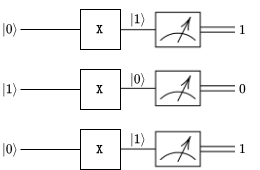
\includegraphics[width=0.85\linewidth]{body/ch4/figs/3-x-gates}
	\caption[Illustrating a Simple Bit Flip Using 3 \texttt{X} gates.]{Single-qubit quantum gates such as the \texttt{X} gate can be implemented directly in FPGA LUTs. This example illustrates a bit flip that would change the output of the LUT from 010 (or INIT[2] on a Xilinx 7-series FPGA) to 101 (INIT[5]).}
	\label{fig:3-x-gates}
\end{figure}

In this case, the data-width of the input and output quantum states is expected to remain the same. Therefore, if all the input and output relations are tabulated, a finite state machine can be used to represent quantum states in gray code to map the transformations for each value in a LUT. Multiple-qubit gates such as \texttt{CNOT} and \texttt{RNOT} gates can be stored directly in the distributed RAM as vectors. The control qubit and target qubits can be stored separately and used as input operands to multiplier and adder IP cores when performing controlled quantum gate operations. Equation \ref{eqn:generic-cnot} implies that memory usage for storing controlled gates of the form $\Lambda Q$ can be reduced by storing a template of the matrix operation with place holder values for the elements labelled $q_{11}$, $q_{12}$, $q_{21}$, $q_{22}$. Using a generic template could lead to potential increases in power usage as more clock cycles of the FPGA would be required to read the template from memory and construct the desired gate by changing the place-holder values.

Recall that to perform a unitary transformation on a $n$-dimensional Hilbert space, the quantum gate operator needs to be a vector space with $2^n \times 2^n$ dimensions. The proposed solution uses DDR SDRAM memory to resolve larger quantum gate operations instead of BRAMs on the FPGA fabric. An AXI manager interface to access data by communicating with vendor provided memory interface IP cores that allow asynchronous read and synchronous write interactions with the DDR SDRAM memory. Notably, DDR3 and DDR4 based RAMs operate at double the clock frequency, providing high data bandwidth, which is suitable for the high-throughput requirements involved in quantum gate operations. 

For example, to perform the \texttt{QFT} subroutine on the 3-qubit register $\ket{011}$, the $2^3 \times 2^3$ matrix demonstrated in equation \ref{eqn:qft-matrix} needs to be multiplied by the Hilbert space of the quantum state in the form
\begin{align}\label{eqn:qft-example-2}
	\texttt{QFT}\ket{011} = \nonumber\\ \frac{1}{\sqrt{8}}\left(\begin{matrix}
		1 & 1 & 1 & 1 & 1 & 1 & 1 & 1\\
		1 & \omega & \omega^2	& \omega^3	& \omega^4	& \omega^5	& \omega^6	&	\omega^7\\
		1 & \omega^2 & \omega^4	& \omega^6	& 1	& \omega^2	& \omega^4	&	\omega^6\\
		1 & \omega^3 & \omega^6	& \omega^1	& \omega^4	& \omega^7	& \omega^2	&	\omega^5\\
		1 & \omega^4 & 1	& \omega^4	& 1	& \omega^4	& 1	&	\omega^4\\
		1 & \omega^5 & \omega^2	& \omega^7	& \omega^4	& \omega	& \omega^6	&	\omega^3\\
		1 & \omega^6 & \omega^4	& \omega^2	& 1	& \omega^6	& \omega^4	&	\omega^2\\
		1 & \omega^7 & \omega^6	& \omega^5	& \omega^4	& \omega^3	& \omega^2	&	\omega^1
	\end{matrix}\right) \left(\begin{matrix}
	0 \\ 0 \\ 0 \\ 1 \\ 0 \\ 0 \\0 \\0 
\end{matrix}\right)
\end{align}
where $\omega = e^{2\pi/8}$. Provided that the elements of the \texttt{QFT} are calculated before pre-loading them in memory, performing the above operation would require 65 multiplications and 64 additions to produce the output. To perform multiplication operations on the proposed hardware, fixed-point parallel multipliers and constant-coefficient multipliers for two's complement signed or unsigned data can be generated using IP cores in FPGA design tools such as Xilinx Vivado for Xilinx FPGAs or Quartus Prime for Intel FPGAs. The total number of multipliers and adders required to model a unitary transformation on a $n$-qubit quantum system can be derived from the above example by observing that the $n$-qubit output $\ket{\psi_f}$ is given by the sum of the product between elements $u_{ij}$ of the unitary matrix $U$ and the elements in the initial quantum state column vector $\psi$, i.e.,
\begin{align}\label{eqn:multipliers+adders}
	\ket{\psi_f}	& = \sum_{j = 1}^{2^n} u_{ij} \cdot \psi_{j}~,~\text{for}~i=1,2,...,2^n
\end{align}
This implies that for quantum gate emulations of $n$-qubit systems:
\begin{itemize}
	\item 
	$2^n$ multipliers are required to handle the product of each element $u_{ij}$ of the $2^n \times 2^n$ unitary transform $U$, with the corresponding $n$ elements from the quantum state vector
	\item
	$2^n - 1$ adders are required to handle the compute the final value of each entry in the state vector of the output state $\ket{\psi_1}$
\end{itemize}
In this design, the proposed hardware architecture performs multiplication operations in pipelined stages. Multiplier pipelines take advantage of the inherent parallelism in FPGA architectures which have dedicated resources for performing fixed-point multiplication such as slice logic and DSP slices. For multiplication of large matrices, the number of pipeline stages needs to selected to satisfy the latency and performance requirements. Parallel multiplication can be optimised by reducing DSP sliced base multiplier utilisation by using an amalgamation of slice logic and dedicated multiplier primitives \cite{xilinx20167series}. The area of LUT-based multipliers such as the ones used for single-qubit gates can be optimised by ensuring that both input operands are unsigned, and that both input operands are smaller than 16 bits. Application of pipelined stages to perform quantum gate operations was expected to introduce latency effects to the system. In this paper, optimal pipelining was achieved using the pipeline registers inside DSP slices of multiplier cores as shown in figure \ref{fig:dsp-opt-pipeline} \cite{xilinx2014multiadder}.
\begin{figure}[!ht]
	\centering
	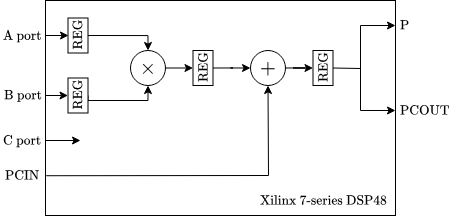
\includegraphics[width=0.80\linewidth]{body/ch4/figs/dsp-opt-pipeline}
	\caption[Illustrating Xilinx 7-Series FPGA DSP48 for Performing Matrix Products Associated with Quantum Gate Operations.]{An illustration of the DSP48 slice implementation which can be used to perform quantum gate operations in the computational basis.}
	\label{fig:dsp-opt-pipeline}
\end{figure}

Since detected quantum states are stored in $m$-bit shift registers, multiplier and adder cores need to support inputs ranging from 1 to $m$-bits wide and outputs ranging from 1 to $2m$ bits wide. The output data width needs to be twice the width of the inputs because multipliers typically produce outputs with larger values that require wider registers to prevent bit overflow errors. Figure \ref{fig:xilinx-vector-multiply} shows an example of a simple vector multiply block with bit staggering. Bit staggering is used to achieve data alignment by ensuring that all inputs are right-justified when passed to the operators inside a multiplier core. Implementation of bit staggering in the architecture ensures that the core works for single or multiple DSP slice applications. Outputs from the different multipliers in the pipeline are cascaded using the \texttt{PCIN} and \texttt{PCOUT} ports.
\begin{figure}[!ht]
	\centering
	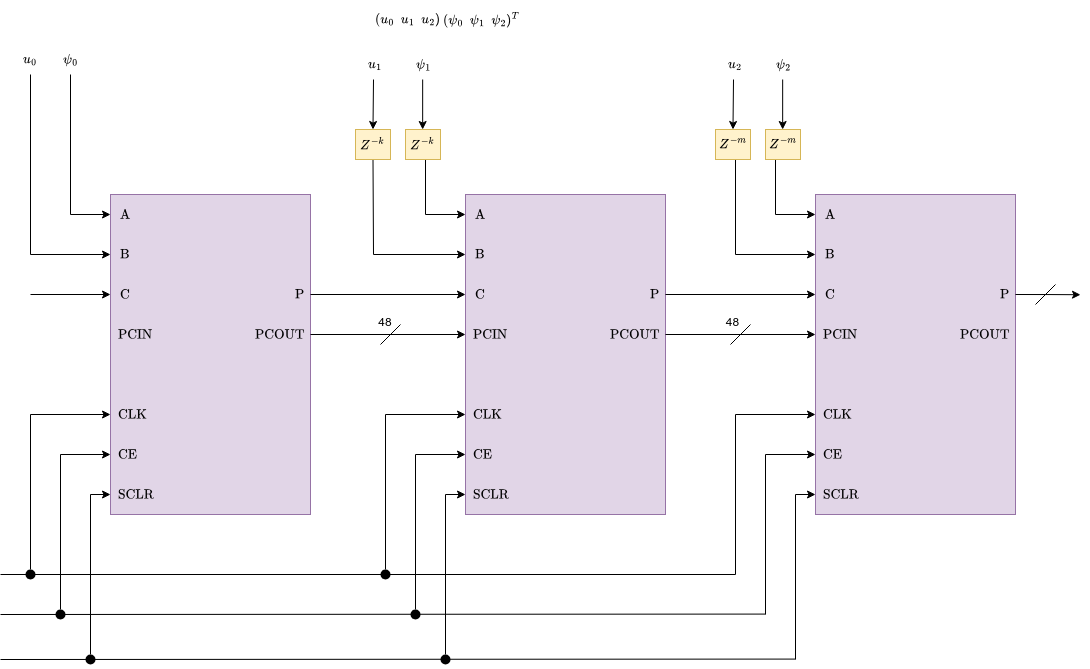
\includegraphics[width=\linewidth]{body/ch4/figs/xilinx-vector-multiply}
	\caption[Simple Vector Multiply Block using the LogiCORE IP Multiply Adder.]{A simple vector multiply for all DSP slice implementations of the Multiply Adder IP core in AMD Vivado and Xilinx 7-series FPGAs \cite{xilinx2015multiplier}. The example shown is implemented to multiply a single row in the unitary matrix of a quantum circuit with the column vector of the quantum state. The output of each multiplication is stored in pipeline registers of DSP slices.}
	\label{fig:xilinx-vector-multiply}
\end{figure}

Constant-coefficient multipliers, which are of crucial for computing products of basis vectors and their normalised amplitudes, can be constructed from distributed memory, block memories, or embedded multipliers \cite{xilinx2015multiplier}. The final output of the FPGA system corresponds to the output of the coefficient multipliers. This output is stored in the distribute RAM transferred to the UIS system, where it can be displayed to the user on the 7 segement display. In the proposed design, quantum gate errors were only considered to the extent of loss in precision due to the use of a fixed-point number scheme.  

\subsubsection{Quantum Teleportation Design Considerations for Hardware Emulation}

Quantum algorithms and quantum circuits are defined implicitly in the data paths, multipliers and adders in the pipeline. Since the pipeline stages use registers, the emulation cannot satisfy the no cloning theorem of qubits in the model as the classical bits that represent quantum states are duplicated for various reasons throughout the implementation. 

The aim of quantum teleportation is to verify the operation of the quantum channel in the context of a QKD network. In that sense, the quantum teleportation algorithm can also be interpreted as a qubit transfer protocol between the classical computer at the source and the quantum computer at the network edge. Furthermore, quantum teleportation circumvents the no cloning constraint on which prevents qubits from being duplicated. This is done by transfer the quantum state to a qubit in an entangled pair across the quantum channel using results from measurements of classical bits.

Literature shows that for Alice to convey $n$-qubits of information to Bob, at least $\lceil n/2\rceil$ qubits must be transmitted and both parties must share an entangled state prior to the initialisation of the communication channel. Requirements for performing the quantum teleportation to transmit key string $x$ can be derived from Cleve et al.'s observation that if the source transmits $n$ qubits to the photosensors, after both parties have shared prior entangled states, then at most $2n$ bits can be stored in the shift registers. If no prior entangled state information is stored, then each qubit sequence that is transmitted produces at most $n$ classical bits. The proposed design focuses on the case where prior entanglement information is shared between both parties.

In the first qubit transmission mode, if asynchronous writes to the FIFO macros are performed on a clock edge, then twice as many clock cycles are required to write sensor data to shift registers in the case where prior entangled state information has been shared. In the case where prior state information has not been shared, $1$ clock cycle would required for every 3 qubits in the system as shown in equation \ref{eqn:number-of-sequences}. Handshaking flags can be transmitted through the bus in the classical channel between the microcontroller and FPGA as previously described. The handshaking signals correspond to the classical measurements in the quantum circuit depicted in figure \ref{fig:quantum-teleportation-circuit}. The quantum gate operation that Bob needs to perform on their half of the EPR pair depends on the signal transmitted through the classical channel in the quantum interface as shown in table \ref{tab:teleportation-table}.

\begin{table}[ht!]
	\centering
	\caption[Table Showing Possible Classical Outputs and Required Quantum Gates for the Quantum Teleportation Circuit.]{Table showing possible classical outputs and the sequence of quantum gates that Bob is required to perform in order to recover the original quantum state at Alice's location.}
	\label{tab:teleportation-table}
	\begin{tabular}{ |c|c|c| } 
		\hline
		\textbf{Classical Output} & \textbf{Gate 1} & \textbf{Gate 2}\\ 
		\hline
		$(00)_2$ & \texttt{I} & \texttt{I} \\ 
		\hline
		$(01)_2$ & \texttt{X} & \texttt{I} \\ 
		\hline
		$(10)_2$ & \texttt{Z} & \texttt{I} \\ 
		\hline
		$(11)_2$ & \texttt{X} & \texttt{Z} \\ 
		\hline
	\end{tabular}
\end{table}

Quantum gates that are involved in the quantum teleportation protocol include the \texttt{CNOT}, \texttt{H}, \texttt{X}, and \texttt{Z} gates as illustrate in the quantum circuit in figure \ref{fig:quantum-teleportation-circuit}. 
\begin{figure}[!ht]
	\centering
	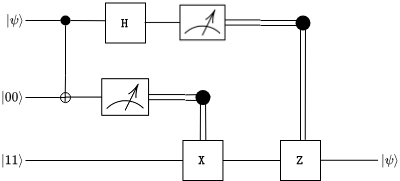
\includegraphics[width=\linewidth]{body/ch4/figs/quantum-teleportation-circuit}
	\caption[Quantum Circuit of the Quantum Teleportation Protocol.]{The quantum teleportation procedure implements \texttt{CNOT}, \texttt{H}, \texttt{X}, and \texttt{Z} gates in a sequence represented by the quantum circuit. The classically controlled quantum gate operations applied in this circuit correspond to the case where Alice measures bit sequence $(11)_2$.}
	\label{fig:quantum-teleportation-circuit}
\end{figure}

The two single gate operations are performed by Bob on the FPGA while the \texttt{CNOT} is performed at the source on the message qubit and one half of the entangle pair. In the proposed model design, the output of the \texttt{CNOT} gate transmitted as is and the matrix operation is not performed on the microcontroller. The result of Alice's state measurement is carried in the \texttt{trigger} and \texttt{ack} signals as a classical two-bit string. In the last stage of the protocol, Bob performs the single-gate operations depending on the classical bits and qubits transmitted from the source to effectively complete the transmission of the key $x$ as qubits. 

The quantum teleportation protocol and overview of required resources are summarised below:
\begin{enumerate}
	\item
	Alice and Bob one half of a previously prepared EPR pair. The qubit at the source is stored as a bit pattern on the microcontroller while Bob's half is stored in the external memory on the FPGA. In the quantum channel circuit, entangle qubits are represented by toggling the LED bit pattern between both qubits in the EPR pair. The FPGA only responds to half of the signal, although qubit detections from the photosensors are not stored during this process.
	\item 
	Alice performs a Bell state measurement to entangle the key $x$ with the entangled half of the EPR pair at the source. The output is transmitted in the \texttt{trigger} signal from the source microcontroller to the end-point FPGA.
	\item 
	Bob performs a series of single-qubit quantum gate operations to recover the key $x$. The output is displayed on the 7 segment display to determine if the transfer was successful.
\end{enumerate}

The proposed implementation uses a finite state machine (FSM) to emulate the quantum teleportation algorithm. Each state in the FSM is mapped to logic cells for emulating single-bit quantum gate operations 
\subsubsection{Simulating the QFT Transform Quantum Circuit}

The QFT can be implemented as an algorithm or a subroutine in the quantum factoring algorithm.In other words, the QFT behaves like a quantum gate, described by the product expansion in the computational basis and the matrix in \ref{eqn:qft-matrix}. 

As a standalone algorithm, the QFT takes in $n$ inputs corresponding and performs a series of quantum gates as shown in figure \ref{fig:nielsen-qft}. To emulate the \texttt{QFT} quantum circuit, vector multiplication are performed and outputs are stored in pipeline registers as illustrated in figure \ref{fig:qft-pipeline} below.
\begin{figure}[!ht]
	\centering
	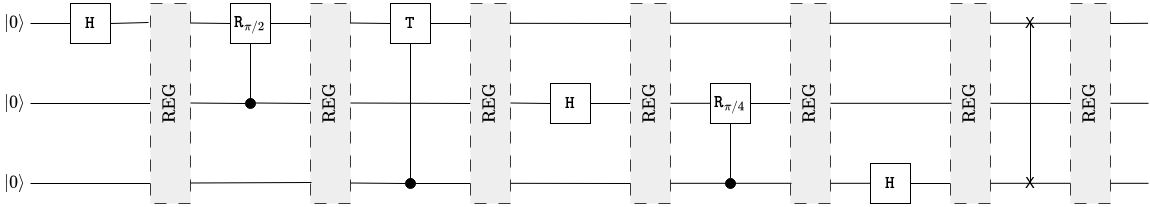
\includegraphics[width=1.0\linewidth]{body/ch4/figs/qft-pipeline}
	\caption[Illustrating the Implementation of DSP Pipeline Registers for Performing the QFT in the QAES.]{Pipeline registers are used to store intermediate results between gate operations. The final output of the quantum circuit is stored in the distribute RAM.}
	\label{fig:qft-pipeline}
\end{figure}

The pipeline can be summarised in the following pseudocode.
\begin{center}
	\textbf{Algorithm: 3-Qubit QFT}
\end{center}
\textbf{Inputs}: 3 qubits $\ket{j_1}$, $\ket{j_2}$, $\ket{j_3}$ initialised to $\ket{0}$\\
\textbf{Outputs}: 3 qubits $\ket{k_0}\ket{k_1}\ket{k_2}$\\
\textbf{Runtime}: $\mathcal{O}(\log_2 N)$

\fbox{%
	\begin{varwidth}{\dimexpr\linewidth-2\fboxsep-2\fboxrule\relax}
		\begin{algorithmic}[1]
			\Procedure{QFT}{$\ket{j_0}$, $\ket{j_1}$, $\ket{j_2}$}
			\State \ \ \ \ //apply Hadamard gate on first qubit
			\State \ \ \ \ \texttt{H} ($\ket{j_0}$); \\
			
			\State \ \ \ \ //apply controlled-$\texttt{R}_{\pi/2}$ with control qubit ~~~~~ $\ket{j_0}$
			\State \ \ \ \ \texttt{controlled\_R} ($\ket{j_1}$, ($\pi/2$, $\ket{j_0}$));\\
			
			\State \ \ \ \ //apply controlled-$\texttt{R}_{\pi/4}$ with control $\ket{j_0}$
			\State \ \ \ \ \texttt{controlled\_R} ($\ket{j_2}$, ($\pi/4$, $\ket{j_0}$));\\
			
			\State \ \ \ \ //apply Hadamard gate on second qubit
			\State \ \ \ \ \texttt{H} ($\ket{j_1}$); \\
			
			\State \ \ \ \ //apply controlled-$\texttt{R}_{\pi/2}$ with control qubit $\ket{q_1}$
			\State \ \ \ \ \texttt{controlled\_R} ($\ket{j_2}$, ($\pi/2$, $\ket{j_1}$));\\
			
			\State \ \ \ \ //apply Hadamard gate on third qubit
			\State \ \ \ \ \texttt{H} ($\ket{j_2}$); \\
			
			\State \ \ \ \ //swap qubits 1 and 3
			\State \ \ \ \ \texttt{swap} ($\ket{k_2}$, $\ket{k_0}$);\\
			
			\State \ \ \ \ \textbf{return} $\ket{k_0}\ket{k_1}\ket{k_2}$;\\
			
			\State \ \ \ \ //reset all qubits:
			\State \ \ \ \ \texttt{reset} ($\ket{j_0}$, $\ket{j_1}$, $\ket{j_2}$);
			\EndProcedure
		\end{algorithmic}
	\end{varwidth}% 
}

The pipeline registers store the data after executing each function in the pseudocode. From the above, it can be seen that 9 pipeline registers are required to perform the 3-qubit QFT. The output of the QFT represents qubits in the Fourier basis state $\ket{+}$ and $\ket{-}$, which can be used to represent the output quantum register $\ket{k_0 k_1 k_2}$ graphically as shown in figure \ref{fig:fourier-basis}. 

\subsubsection{Quantum Factoring Algorithm}

As shown in section \ref{subsubsec:q-shors-algo}, the quantum factoring algorithm applies principles of phase estimation using the inverse QFT to determine the period of an integer. This is useful for cracking the RSA public-key encryption pattern which generates a public-private key pair using two large prime numbers $p_1$ and $p_2$. Cracking the RSA pattern involves factorising a given large prime product $N = p_1 p_2$ in order to calculate the private key in the pair. The aim of the proposed design is to factor the integer $N = 21$ into the prime factors 3 and 7 using Shor's factoring algorithm. 

Given the integer $N$ to be factored, Shor's algorithm begins by choosing a random integer $x$ less than $N$ and coprime to $N$. Then, the algorithm finds the order $r$ of $N$ such that $x^r \equiv1\left(\text{mod}~N\right)$. The number of qubits $n$ is 
\begin{align}\label{eqn:shor-required-bits}
	n	& = \lceil \log_2 N\rceil
\end{align}
To factor the number $N = 21$, a total of 5 qubits is required to perform the operation. Three qubits form the control register and the other two qubits form part of work register. The inverse QFT, which is equivalent to applying the QFT circuit in reverse, is used to change to transform the first qubit register to the computational basis after applying Hadamard gates to each qubit.
\begin{figure}[!ht]
	\centering
	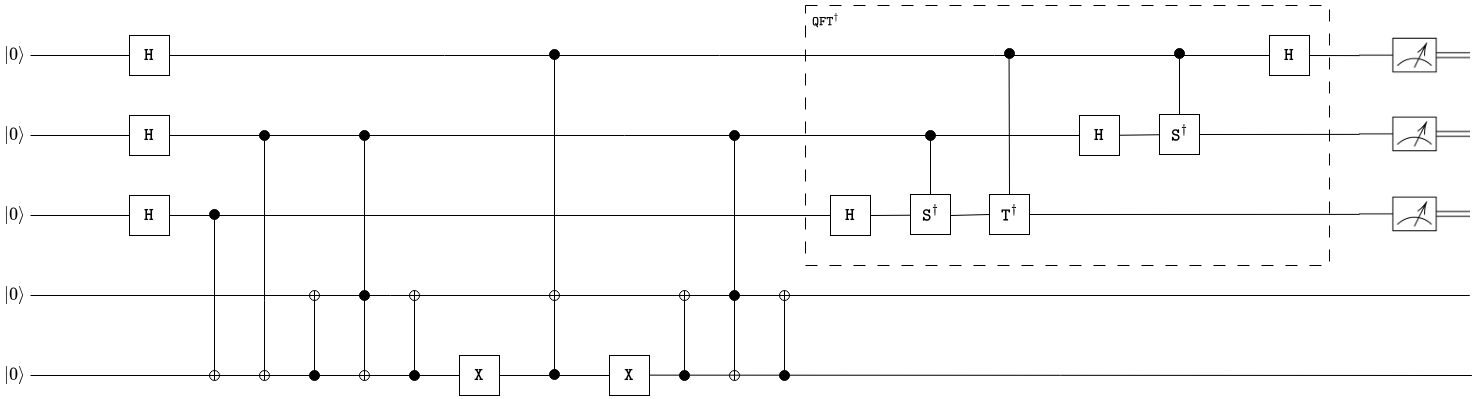
\includegraphics[width=1.0\linewidth]{body/ch4/figs/quantum-factoring-algorithm}
	\caption[Quantum Circuit Representation of the Emulated Quantum Factoring Algorithm for $N = 21$ and $a=4$.]{Showing the 5-Qubit quantum circuit for factoring $N=21$ and $x=4$  which applies the inverse QFT ($\texttt{QFT}^\dagger$) \cite{skosana2021demonstration}. The expected order of $N$ when $x = 4$ is $r$, which can be extracted from the output of the control register given by $2^n s/r$, where $s \in \mathbb{Z}$ is randomly assigned according to the measurement of the control register outputs.}
	\label{fig:quantum-factoring-algorithm}
\end{figure}

In this paper, simulation of the quantum factoring or (Shor's) algorithm for solving the order-finding problem is performed in relation to the quantum circuit shown in figure \ref{fig:quantum-factoring-algorithm}. When fully expanded, the quantum circuit shows that to successfully emulate the quantum factoring algorithm for $N = 21$ with an initial guess of $x = 4$, the system requires:
\begin{itemize}
	\item 
	25 \texttt{CNOT} gates
	\item 
	8 Hadamard gates
	\item 
	2 explicit \texttt{X} gates
	\item 
	2 controlled-$\texttt{R}_{\pi/2}$ gates
	\item 
	13 controlled-$\texttt{R}_{\pi/4}$ gate
\end{itemize}
Similar to the implementation of the QFT algorithm above, the quantum circuit is pipeline to store the state of the simulated qubits after each quantum gate operation. The circuit depth of Shor's algorithm is high due to the large number of quantum gates required to perform the procedure. This implies that the emulated quantum circuit also long critical path on the FPGA fabric, which leads to high latency and reduced performance. Additionally, storage, latency and power requirements are increased by pipelining the execution of the algorithm. Therefore, emulation of the quantum factoring algorithm for small integers such as $21$ is not expected to offer performance gains over PC-based simulations of the quantum factoring algorithm. 

In this implementation, the possible quantum states of the working register are encoded as follows:
\begin{align}\label{eqn:shor-work-register}
	\ket{1}_{10} \rightarrowtail \ket{00}_{2}\nonumber\\
	\ket{4}_{10} \rightarrowtail \ket{01}_{2}\nonumber\\
	\ket{16}_{10} \rightarrowtail \ket{11}_{2}
\end{align}
so that instead of evaluating $4^r~\text{mod}~21$, the quantum algorithm evaluates $\log_4(4^r~\text{mod}~21)$ \cite{skosana2021demonstration}. Given that $x = 4$, possible values of $r$ can be calculated from
\begin{align}
	4^0	& = 1~\mod 21\nonumber\\
	4^1	& = 4~\mod 21\nonumber\\
	4^2	& = 16~\mod 21\nonumber\\
	4^3	& = 1~\mod 21\nonumber\\
\end{align}
which shows that the period of $N = 21$ is 3 \cite{skosana2021demonstration}. Measurement of the control register output yields a probability distribution with peaks that correspond to values of $2^n \sigma/r$, where $\sigma$ is a randomly assigned number associated with measurement probabilities.

\subsubsection{Emulation of Grover's Algorithm}

The aim of the quantum search algorithm, or Grover's algorithm, is to find the solution $a$ of a function $f(x)$ that produces an outcome of 1. This can be used to find the index of an item in a database that matches given criteria labelled $x_0$. As mentioned in section \ref{subsubsec:q-search-algo}, the main advantage of using the quantum search algorithm is that it performs the entire search of a $N$-entry database in $\mathcal{O}(\sqrt{N})$, compared to sequential classical algorithms which perform the search $\mathcal{O}(N)$ time. 

For this implementation of the quantum search algorithm, a database with $N = 4$ entries as shown in table \ref{tab:grover-entries} where each item is indexed from 0 to 3. This implies that the emulated quantum computer only needs to represent two qubit registers in the hardware. 

\begin{table}[ht!]
	\centering
	\caption[Table Showing Indices and their Associated Strings for Performing the Quantum Search Algorithm.]{Table of two-qubit registers indices and their associated strings for performing the quantum search algorithm (QSA).}
	\label{tab:grover-entries}
	\begin{tabular}{ |c|c|c| } 
		\hline
		\textbf{Index} & \textbf{Name} & \textbf{QSA Output}\\ 
		\hline
		$\ket{00}_2$ & Kestrel & $\ket{00}_2$ \\ 
		\hline
		$\ket{01}_2$ & Kite & $\ket{00}_2$ \\ 
		\hline
		$\ket{10}_2$ & Harrier & $\ket{00}_2$ \\ 
		\hline
		$\ket{11}_2$ & Goshawk & $\ket{11}_2$ \\ 
		\hline
	\end{tabular}
\end{table}

Figure \ref{fig:grovers-circuit} shows the quantum circuit representation of the quantum search algorithm which consists of:
\begin{itemize}
	\item 
	6 Hadamard gates
	\item 
	2 Pauli-Z gates
	\item 
	2 Controlled-\texttt{Z} gates (\texttt{CZ})
\end{itemize}
\begin{figure}[!ht]
	\centering
	\includegraphics[width=1.0\linewidth]{body/ch4/figs/grovers-circuit}
	\caption[Quantum Circuit for Finding the Index of an Entry in a Database.]{The quantum circuit representation of the quantum search algorithm for finding the element in the index corresponding to the state $\ket{11}$.}
	\label{fig:grovers-circuit}
\end{figure}
The controlled-\texttt{Z} gates plays the role of the oracle in the Grover's iterative. Using the quantum information system equivalent of a truth table as shown in \ref{tab:controlled-z}, the outputs of the this two-qubit input gate can be seen more clearly. In the case where the input to the \texttt{CZ} gate is $\ket{11}$, the phase of the qubit is flipped as illustrated by the unit circle representation of the two-qubit register in figure \ref{fig:grover-phase-flip}.
\begin{figure}[!ht]
	\centering
	\includegraphics[width=1.0\linewidth]{body/ch4/figs/grover-phase-flip}
	\caption[Graphical Representation of the Controlled-Z Gate Applied in the Quantum Oracle of Grover's Search Algorithm.]{A unit circle representation of the application of the \texttt{CZ} gate to a quantum register which has an original state of $\ket{11}$ depicted in red. The expected output in this case is  $-\ket{11}$ depicted in blue.}
	\label{fig:grover-phase-flip}
\end{figure}
\begin{table}[ht!]
	\centering
	\caption[Table Showing the Input-and-Output Relationship of the \texttt{CZ} Gate in a Two-Qubit System.]{Input-and-output relationship for \texttt{CZ} gate shown as a quantum truth table.}
	\label{tab:grover-phase-flip}
	\begin{tabular}{ |c|c|c|c| } 
		\hline
		\textbf{Input} & \textbf{Control} & \textbf{Target} & \textbf{Output}\\ 
		\hline
		$\ket{00}_2$ & $\ket{0} $& $\ket{0}$ & $\ket{00}_2$  \\ 
		\hline
		$\ket{01}_2$ & $\ket{0}$ & $\ket{1}$ & $\ket{01}_2$ \\ 
		\hline
		$\ket{10}_2$ & $\ket{1}$ & $\ket{0}$ & $\ket{10}_2$ \\ 
		\hline
		$\ket{11}_2$ & $\ket{1}$ & $\ket{1}$ & -$\ket{11}_2$ \\ 
		\hline
	\end{tabular}
\end{table}
The corresponding high-level description for implementing the \texttt{CZ} gate using MATLAB matrix operations is given by
\begin{align}
	\left(\begin{matrix}
		1	 &	0	& 0 & 0\\
		0	 &	1	& 0 & 0\\	
		0	 &	0	& 1 & 0\\
		0	 &	0	& 0 & -1\\	
	\end{matrix}\right)\cdot\left(\begin{matrix}
	0 \\ 0 \\ 0 \\ 1
\end{matrix}\right)
\end{align}
The quantum circuit needs one iteration to find the solution, regardless of the position of the entry in the database. For demonstration purposes, the algorithm is implemented to find the index corresponding to the state $\ket{11}$. This result corresponds to the classical output registers at the end of a single iteration of the illustrated quantum circuit.

The proposed application of the search algorithm has a low circuit depth compared to the application of Shor's factoring algorithm as described in the previous subsection. A lower circuit depth indicates lower latency when emulating the algorithm in the fabric of the FPGA. In this paper, results of the execution of the quantum search algorithm are compared to the execution time of a sequential search algorithm that finds uses simple conditional statements to determine find $x_0$. 
 
\subsection{Design Tools and Workflow}

The following shows the design flow of the FPGA emulated quantum computer and quantum interface, including some of the tools used in the development of the integrated system.  

To initialise qubits and model laser pulses through LED status changes, the proposed design uses the ARM-based STM32F051C6 microcontroller due to its simple architecture and multiple GPIO pins for generating the required signals for driving LEDs as seen in figure \ref{fig:stm32-devboard}. The STM32 processor is a 32-bit processor which offers enhanced system debug with breakpoint and trace capabilities, as well as low power consumption and platform security. 
\begin{figure}[!ht]
	\centering
	\includegraphics[width=0.30\linewidth]{body/ch4/figs/stm32-devboard}
	\caption[Image of the UCT STM32F0 Development Board Used to Model the Behaviour of a Laser-Based Flying-Qubit Transmitter.]{Image of the UCT STM32F0 daughter board used to model the behaviour of a laser-based flying-qubit transmitter in the SPQIS and FQDS subsystems}.
	\label{fig:stm32-devboard}
\end{figure} 

The first iteration of the electronic circuit for modelling the quantum channel is built on a breadboard. Following verification of output voltages and currents, the final design was built on veroboard due to its low cost.

Quantum circuits are emulated on the Nexys A7 FPGA board (shown in figure \ref{fig:nexys-a7}) which is designed around the Xilinx Artix-7 FPGA family. The board was selected for its ready-to-use digital circuit, versatile interfaces and vast resources which can reduce development time. Additionally, the board is compatible with the AMD Vivado design suite which provides a graphical representation of the circuit and IP cores that can be used to map quantum algorithms to hardware in the synthesis stage of development. Vivado also offers automatic optimisations of placement, routing and clock frequencies in the hardware design. 
\begin{figure}[!ht]
	\centering
	\includegraphics[width=0.55\linewidth]{body/ch4/figs/nexys-a7}
	\caption[Nexys A7 Board based on the Xilinx 7-Series FPGAs.]{Image of the Nexys A7 board which is based on the Artix-7 series \cite{diligent2024nexysa7}.}
	\label{fig:nexys-a7}
\end{figure}

Before synthesis, algorithms are modelled and tested using MATLAB, Simulink and SystemVerilog simulations. Python simulations of quantum circuits using the Qiskit Runtime service are used to benchmark the performance of the emulated quantum computer. 

\subsubsection*{High-Level Abstraction}

The high-level design abstraction gives the detailed behaviour and executable description of what the what the system does. This is written in high level coding languages such as embedded C, MATLAB and Python. Specifically, the behaviour of the flying-qubit transmitters is described in embedded C and uploaded to the STM32 microcontroller through the serial wire debug interface. The microcontroller board also contains a ST-LINK debugger circuit which can be used to troubleshoot any behavioural issues in operation of the SPQIS and FQDS modules. 

MATLAB is used to fully describe quantum algorithm using element-wise matrix operations to ensure that the behaviour can be efficiently mapped to the logic elements of the FPGA. MATLAB was chosen due to the large suit of modelling tools provided by MathWorks which can reduce development time significantly. Some of the tools used in this proposal include Simulink for modelling quantum circuits as well as IP cores that are compatible with Xilinx 7-series FPGAs and AMD Vivado.

The following includes the high-level design workflow for the microcontroller and FPGA:
\begin{itemize}
	\item 
	Atollic TRUEStudio C/C++ IDE for STM32 is used to model qubit initialisation and laser pulse sequences through bitmaps that control LED status changes. 
	\item 
	Quantum gates are formulated as vector multiplication functions using MATLAB scripts in MATLAB 2024a.
	\item 
	Quantum algorithms are represented as quantum circuits and pseudocode as described above.
	\item 
	Quantum circuits are constructed by combining the appropriate functions representing quantum gate operations.
	\item 
	Code is converted to Simulink models for directing mapping of algorithm and quantum circuit pipelines to hardware components using IP cores.	
\end{itemize}

\subsubsection*{RTL Code Design and Verification}

The digital design of the quantum computer emulator relies on the SystemVerilog hardware description language to describe the register-transfer level behaviour of the FPGA board. HDLs such as VHDL, Verilog and SystemVerilog are connected to simulators and synthesis tools that generate logic implementations and understand the semantics of hardware \cite{wolf2004fpga}. SystemVerilog code was considered for its simplicity and extended capabilities compared to VHDL and Verilog. A combination of manual and automated code-writing techniques were considered in order to reduce development time. Using the automated technique, MATLAB algorithm is converted to SystemVerilog in the HDL Coder tool. 

The following items show the use of various tools in the RTL coding development phase of the quantum emulator:
\begin{itemize}
	\item 
	Each SystemVerilog module has an accompanying testbench which is simulated using Vivado's built in simulations tools.
	\item 
	HDL Verifier was used in MATLAB to perform further tests and simulations of quantum circuits.
	\item 
	Gate level simulations are performed to verify timing and logic correctness. HDL Verifier is used in MATLAB to verify correct functionality. 
\end{itemize}

\subsubsection*{Synthesis}

The synthesis stage of the design workflow translates the verified RTL description into a gate-level netlist that can be used to program the FPGA. Using the Vivado design suite, the SystemVerilog modules are synthesised into logic gates and other hardware resources. Synthesis tools use LUTs to implement any function of $n$-qubits corresponding the number of LUT inputs. The aim of the synthesis tool is to perform the Boolean function describing the quantum operation with a minimum number of nodes in the network of the FPGA fabric using technology-mapping algorithms to generate bitstreams. The generated bitstream file is used to configure the FPGA with the desired logic. Additionally, pipeline directives are applied to enhance the performance of key arithmetic components, such as DSP slices, ensuring efficient execution of quantum operations. This step optimizes resource usage and prepares the design for hardware implementation using:

\begin{itemize}
	\item 
	A gate level netlist generated in a bitstream using Vivado to synthesise the HDL code.
	\item 
	Pipeline directives are used to optimise the performance of DSP slices and other arithmetic components such as multipliers and.
\end{itemize}

\subsubsection*{Design Testing and Verification}

Design testing and verification are essential steps in ensuring that the FPGA-based quantum computer emulator functions as intended. Various methods are employed to test the operation of individual components, such as the microcontroller, quantum channel, and photoresistors, as well as the integrated system as a whole. Simulations, hardware tests, and measurements are used to verify proper signal processing, communication, and the correct execution of quantum algorithms. The following steps outline key aspects of the testing and verification process:

\begin{itemize}
	\item 
	Physical wire voltages and currents are measured on the model quantum channel to ensure that LVCMOS 3.3V or LVTTL 3.3 logical conventions are met
	\item 
	Operation of the microntroller is tested to ensure that qubit sequences are transmitted accurately
	\item 
	Operation of photosensors connected to Pmod ports is tested on the FPGA using SystemVerilog simulations and the built-in Vivado HDL simulator.
	\item 
	Quantum teleportation algorithm is used to verify the operation of the quantum channel based on the two modes of qubit transmission and communication via classical channel signals.
	\item 
	Quantum gate operations and quantum algorithms are tested on actual FPGA hardware using photosensor detections as inputs for initialising qubits in the emulator.\\
	\item 
	The Integrated Logic Analyser (ILA) is used to probe signals and debug the FPGA.
	\item 
	Ensure that the FPGA design integrates suitably with external components.
\end{itemize}

This comprehensive testing and verification strategy ensures that the quantum emulator operates as expected, from the initialization of qubits to the execution of quantum algorithms on FPGA hardware.

\section{Summary}

The methodology for the project revolves around the design, simulation, and implementation of a quantum computer emulator on an FPGA. The key components of the methodology are divided into phases, each of which focuses on specific aspects of the system, such as the initialization of qubits, the emulation of quantum gates, and the testing of the quantum interface.

The design process begins by identifying system requirements, including user and functional requirements. The system is then modularized into subsystems: the Single-Photon Qubit Initialization Subsystem (SPQIS), the Flying Qubit Detection Subsystem (FQDS), the Quantum Algorithm Emulation Subsystem (QAES), and the User Interface Subsystem (UIS). Each subsystem has distinct responsibilities, such as qubit initialization, quantum state detection, quantum algorithm emulation, and system interaction through a user interface.

Once modularization is established, quantum gates and algorithms are mapped to hardware elements on the FPGA, with emphasis on resource management and efficient implementation. Simulations using MATLAB and SystemVerilog aid in verifying functionality before synthesis and physical testing. Distributed RAM and FIFO structures are utilized for storing qubits on the FPGA, with specific attention to performance metrics like transmission rates and power consumption.

Testing and verification involve evaluating the system’s ability to transmit, detect, and emulate quantum operations accurately. Physical measurements are made on wire voltages, currents, and photoresistors, while SystemVerilog and Vivado simulations are employed to verify correct functionality.

Subsequent chapters detail a case study of the proposed design and the accompanying results and conclusions. 

%@@@@@@ Chapter 5 - Design Case Study @@@@@@@@@@@@@@@@@@@@@@@@@@@@@@@@@@@@@@
\chapter{\label{ch:ch5} Design Case Study}

\section{Design Specifications \label{sec:design-specs}}

The methodology and design considerations described in the previous chapter were implemented in a case study design as reported in following chapter. The chapter begins with a description of the specifications of each subsystem and follows with the acceptance test procedures (ATPs) for each subsystem before concluding with the integration test procedures. The first section specifies the hardware components and operation of the SPQIS which involves the 32-bit microntroller and a set of timing constraints for modelling the decoherence times of the initialised qubits. Normalised qubit probabilites were generated in MATLAB and preloaded to the devices to ensure that the probabilistic nature of quantum computers is maintained. 

The FQDS specifications include details about the electronic circuit used to model the quantum channel. The parameters of particular interest include the input and output voltages, current, resistances as well as the physical layout of the design. Since the electronic circuit also includes a NPN-type BJT, other paramaters such as base, collector and emitter voltages and currents are included to characterise the FQDS. 

High-level descriptions of quantum algorithms in MATLAB are specified in the QAES specifications section. This sections also shows snippets of SystemVerilog code used to simulate the RTL behaviour of the system. Further information is provided on the AMD Vivado IP Cores and other resources utilised during the emulation of the quantum algorithms on the Nexys A7 FPGA. The quantum algorithms explored in the design case study included the quantum teleportation algorithm for transferring quantum state information through a quantum channel, the QFT for changing between the computational basis and the Fourier basis, as well as the quantum factoring and quantum search algorithms. Specifically, the case study for emulating the quantum factoring algorithm involved finding the order $r$ of $N = 21$ with an initial guess of $x = 4$, using the quantum circuit in \ref{fig:quantum-factoring-algorithm}. Depending on the quantum circuit and the algorithm performed, quantum gate operations were implemented as FSM or as matrix multiplication operations. 

Specifications of the UIS detail steps for operating each subsystem. In line with quantum mechanical constraints on observations of quantum states, users can prepare initial qubit states and measure the quantum circuit outputs but do not have access to intermediate results from quantum gate operations. Hence, the section on the UIS specification includes instructions for initialising qubits on the microcontroller, selection of the desired quantum circuit emulation experiment, and the manner in which outputs are displayed to the user. 

\subsection{Single-Photon Qubit Initialisation Subsystem Specifications \label{subsec:sqpis-specs}}

\subsubsection{Generate a Normalised Distribution of Probabilities $n$-Qubit Systems}

To maintain the probabilistic nature of quantum computers across the simulation, pure quantum state probabilities were generated using the MATLAB \texttt{randn} function to return normally distributed random numbers as seen in listing \ref{lst:normally-distributed-probabilities} showing a code snippet of the \texttt{generate\_probs} function. In this study of the proposed design, the first qubit in the $n$-qubit quantum register $\ket{q_0 q_1 ... q_{n-1}}$ is the MSB and the last qubit $\ket{q_{n-1}}$ in the register is taken as the LSB. 

\begin{lstlisting}[language=Matlab, caption={MATLAB script for generating pseudo random numbers for the probabilities associated with quantum states.}, label={lst:normally-distributed-probabilities}]
	function amplitude_squared = generate_probs(n)
	
	% The total number of possible states for n qubits is 2^n
	num_states = 2^n;
	
	% Generate the random values using the pseudorandom generator
	random_values = randn(1, num_states);
	
	% Take the absolute values to ensure non-negative probabilities
	abs_values = abs(random_values);
	
	% Normalise the values to make them valid probabilities (sum to 1)
	amplitude_squared = abs_values / sum(abs_values);
	
	% Display the probabilities
	disp('Generated Quantum State Probabilities:');
	disp(amplitude_squared);
	end
\end{lstlisting}

The \texttt{generate\_probs} function takes in the number of qubits $n$ to create $2^n$ probabilities. Since probabilities are the normalised magnitudes of pure (real) quantum states, the built-in \texttt{abs} is used to ensure that the generated probabilities are positive. The table indicates the number of qubits that are initialised for each quantum algorithm and the generated probabilities. Since most qubit registers are initialised in the ground state, the outputs of the \texttt{generate\_probs} function that are valid for this application are such that the probability of measuring the ground state is the greatest. 

Selection of the probabilities introduces deterministic effects in the model which is not ideal for this case study. Therefore, the acceptance test for \texttt{generate\_probs} function needs to verify that the pseudo-random selection process generates normalised values. The output of the \texttt{generate\_probs} is transferred to the STM32 microcontroller and the Nexys A7 FPGA in the FQDS subsystem. 

\subsubsection{Initialise Qubits on the STM32 Microcontroller Using Push-Buttons}

The UCT STM32F0 Development Board employed in the case study is an entry-level 32-bit ARM microcontroller unit which incorporates the Corext-M0 processor designed for a variety of embedded systems applications. Specifically, the  STM32F0 board contains a Cortex-M0 processor which implements a 3-stage pipeline ARMv6-M von Neumann architecture with internal memory. The microcontroller is powered through a standard USB connection which provides a 5V regulated supply of up to 500 mA. When power is supplied to the board, a green LED on the board turns on to indicate to the user that the board is operational. Table \ref{tab:microcontroller-power} shows further hardware specifications for ensuring that the device is operating correctly. 
\begin{table}[ht!]
	\centering
	\caption[Table Showing the Hardware Specifications of the STM32F0 Microcontroller Used to Initialise Qubits and Control Flying-Qubit Emissions.]{Table showing the hardware specifications of the STM32F0 microcontroller used to initialise qubits and control flying-qubit transmissions.}
	\label{tab:microcontroller-power}
	\setlength\tabcolsep{0pt} % let LaTeX compute intercolumn whitespace
	\footnotesize\centering
	\begin{tabular*}{\columnwidth}{@{\extracolsep{\fill}}|c|l|l|}
		\hline
		\textbf{Callout} & \textbf{Description} & \textbf{Value}\\
		\hline
		1		& Input Power & $\SI{5.0}{\volt}$;$\SI{500}{\milli\ampere}$\\
		\hline
		2		& Operating Voltage  & $\SI{2.0}{\volt}$ to $\SI{3.6}{\volt}$\\
		\hline
		3		& Maximum Clock Frequency  &	$\SI{48}{\mega\hertz}$  \\
		\hline
		4		& Operating Temperature	   &	$-\SI{40}{\degreeCelsius}$ to $\SI{85}{\degreeCelsius}$\\
		\hline
	\end{tabular*}
\end{table}

The processor is connected to multiple external peripherals and circuits. An ST-LINK/V2 in-circuit debugger connects to the STM32F051C6 daughter board though the serial wire debug interface that allows code to be compiled, uploaded and stepped through to fix runtime errors. In this case study, quantum state probabilities produced by the \texttt{generate\_probs} MATLAB script are written in a C header file (\textit{quantum\_state.h}) and uploaded to flash memory through the serial wire debug interface as shown in the code snippet in listing \ref{lst:upload-probabilities}. In particular, the snippet shows the initialisation of qubits to the ground state whereby the real amplitude of the $\ket{0}^{\otimes n}$ state is set to 1, corresponding to a normalised probability of 1. 
\begin{lstlisting}[language=C, caption={Snippet code from C header file for initialising qubits in the STM32 microcontroller.}, label={lst:upload-probabilities}]
	// Define a complex number structure to represent quantum amplitudes
	typedef struct {
		float real;    // Real part of the amplitude
		float imag;    // Imaginary part of the amplitude
	} complex_t;
	
	//====================================================================
	// GLOBAL VARIABLES FOR QUANTUM STATES
	//--------------------------------------------------------------------
	
	// 1-qubit quantum register (2 possible states: 
	//|0> and |1>)
	complex_t quantum_state_1q[2] = {
		{1.0, 0.0},  // Amplitude of |0> state
		{0.0, 0.0}   // Amplitude of |1> state
	};
	
	// 2-qubit quantum register (4 possible states: 
	//|00>, |01>, |10>, |11>)
	complex_t quantum_state_2q[4] = {
		{1.0, 0.0},  // Amplitude of |00> state
		{0.0, 0.0},  // Amplitude of |01> state
		{0.0, 0.0},  // Amplitude of |10> state
		{0.0, 0.0}   // Amplitude of |11> state
	};

	// ... remove code blocks for up to 5-qubits
	
	void initQuantumState(complex_t* state, uint8_t num_states);
\end{lstlisting}
The code in \ref{lst:upload-probabilities} hosts a function, named \texttt{initQuantumState} for initialising the qubits to a fiduciary state depending on the selected quantum algorithm. Since the quantum algorithms performed require up to 5-qubits, the \texttt{initQuantumState} function can initialise qubit registers with up to $n = 5$ qubits. If a quantum algorithm is not selected or the board is reset, then the system automatically initialises the two-qubit register $\ket{00}$. Note that on the microcontroller, qubit initialisations represent the set of the monochromatic laser for transmitting single-photon qubits through the quantum channel in the FQDS subsystem. 

In addition to initialising fiduciary state, the SPQIS allows users to prepare entangled qubits for performing the quantum teleportation algorithm as shown in code listing \ref{lst:prepare-entangled-state}.

\begin{lstlisting}[language=C, caption={Further code from the \textit{quantum\_state.h} C header file for peparing EPR pairs.}, label={lst:prepare-entangled-state}]
	// ... removed code block
	
	// Function to prepare an entangled quantum state pair (Bell state)
	void prepareEntangledPair(complex_t* state);
	
	// Prepare an entangled quantum state pair 
	// (Bell state |+> = (|00> + |11>) / sqrt{2})
	void prepareEntangledPair(complex_t* state) {
		float norm = 1.0 / sqrt(2);  // Normalisation factor (1/sqrt{2})
		
		// Set the amplitudes for the Bell state
		// |+> = (|00> + |11>) / sqrt{2}
		state[0].real = norm;  // Amplitude of |00>
		state[0].imag = 0.0;
		
		state[3].real = norm;  // Amplitude of |11>
		state[3].imag = 0.0;
		
		// Set other states' amplitudes to 0 (|01> and |10>)
		state[1].real = 0.0;   // Amplitude of |01>
		state[1].imag = 0.0;
		
		state[2].real = 0.0;   // Amplitude of |10>
		state[2].imag = 0.0;
	}
	#endif /* QUANTUM_STATE_H */
\end{lstlisting}
This \texttt{prepareEntangledPair} function is used during emulation of the quantum teleportation algorithm in which prior entanglement information is shared between Alice and Bob. When the microcontroller is reset or restarted, qubits return to the separable ground state. 
 
\subsection{Flying-Qubit Detection Subsystem Specifications \label{subsec:fqds-specs}}

The pins of the microcontroller are illustrated in figure \ref{fig:stm32-pins}. The design case study uses these pins to model the quantum interface which facilitates quantum and classical communication between the microcontroller and the quantum computer emulated on the FPGA. 
\begin{figure}[!ht]
	\centering
	\includegraphics[width=0.90\linewidth]{body/ch5/figs/stm32f051c6}
	\caption[Showing Input and Output Pins on the STM32 Microcontroller.]{The input and output pins on the microcontroller are implemented in the model of the quantum interface which consists of a quantum channel and classical channel.}
	\label{fig:stm32-pins}
\end{figure}
The system uses 8 LEDs to model monochromatic lasers pulses. The LEDs are connected to the microcontroller through GPIO port B as shown in the table \ref{tab:led-connections}. 
\begin{table}[ht!]
	\caption[Table Showing LED Connections to the STM32 Microcontroller.]{Table showing the fixed relationship between laser-modelling LEDs and GPIO port B pins of the microcontroller.}
	\label{tab:led-connections}
	\setlength\tabcolsep{0pt} % let LaTeX compute intercolumn whitespace
	\footnotesize\centering
	\begin{tabular*}{0.45\columnwidth}{@{\extracolsep{\fill}}|c|c|}
		\hline
		\textbf{LED Label} & \textbf{GPIO Pin~~~~~~~~~}\\
		\hline
		L0		& PB7 \\
		\hline
		L1		& PB6 \\
		\hline
		L2		& PB5 \\
		\hline
		L3		& PB4	 \\
		\hline
		L4		& PB3 \\
		\hline
		L5		& PB2	 \\
		\hline
		L6		& PB1	 \\
		\hline
		L7		& PB0	 \\
		\hline
	\end{tabular*}
\end{table}

The function called \texttt{initGPIO}, as seen in listing \ref{lst:init-port-b}, is used to enable the clock and mode registers for port B as an output for modelling transmissions of single-qubit quantum states. Note that port A is enabled as an input so that buttons can be used to initialise the required ground states for each quantum algorithm. 
\begin{lstlisting}[language=C, caption={Showing the \texttt{initGPIO} function for enabling ports B as a outputs and ports A as inputs.}, label={lst:init-port-b}]
void initGPIO() {
	uint32_t *RCCADDR = (uint32_t*)(0x40021000 + 0x14);
	
	*RCCADDR |= 0b1 << 18;  // Enable clock for port B
	*RCCADDR |= 0b1 << 17;  // Enable clock for port A
	
	// Enable mode register for port B as output (for LEDs)
	GPIOB->MODER |= GPIO_MODER_MODER0_0;
	GPIOB->MODER |= GPIO_MODER_MODER1_0;
	GPIOB->MODER |= GPIO_MODER_MODER2_0;
	GPIOB->MODER |= GPIO_MODER_MODER3_0;
	GPIOB->MODER |= GPIO_MODER_MODER4_0;
	GPIOB->MODER |= GPIO_MODER_MODER5_0;
	GPIOB->MODER |= GPIO_MODER_MODER6_0;
	GPIOB->MODER |= GPIO_MODER_MODER7_0;
	
	// Set mode register for port A as input (for switches)
	GPIOA->MODER &= ~GPIO_MODER_MODER0_0;
	GPIOA->MODER &= ~GPIO_MODER_MODER1_0;
	GPIOA->MODER &= ~GPIO_MODER_MODER2_0;
	GPIOA->MODER &= ~GPIO_MODER_MODER3_0;
	
	// Enable pull-up resistors for switches
	GPIOA->PUPDR |= GPIO_PUPDR_PUPDR0_0;
	GPIOA->PUPDR |= GPIO_PUPDR_PUPDR1_0;
	GPIOA->PUPDR |= GPIO_PUPDR_PUPDR2_0;
	GPIOA->PUPDR |= GPIO_PUPDR_PUPDR3_0;
}
\end{lstlisting}

\subsubsection{Transmit Qubits in the Quantum Channel of the Quantum Interface}

Table \ref{tab:led-connections} indicates that using the first mode of transmission, the system can transmit quantum registers with up to 8 qubits in total. To model qubit registers in the computational basis, bit patterns are transferred to the 8-bit mode registers for GPIO port B as shown in table \ref{tab:mode-1-qubits}. The table shows the number of qubits in the register, the quantum state register with probability 1 that is to be transmitted, and the expected number of sequences $s_1$ to be transmitted. Base on table \ref{tab:led-connections}, it can be seen that the L0 is associated with the LSB and L7 is associated with the MSB. Therefore, bit patterns need to be reversed in order to transfer qubits accurately through the system. The pattern column in \ref{tab:mode-1-qubits} shows the decimal conversion of the reversed bit pattern.
\begin{table}[ht!]
	\caption[Table Showing the Transmitted Flying-Qubit Registers Using Transmission Mode 1.]{Table showing the number $n$ of qubits in the register, qubits in the register, transmitted bit pattern as a decimal number, and the expected number of sequences $s_1$.}
	\label{tab:mode-1-qubits}
	\setlength\tabcolsep{0pt} % let LaTeX compute intercolumn whitespace
	\footnotesize\centering
	\begin{tabular*}{0.8\columnwidth}{@{\extracolsep{\fill}}|c|c|l|l|}
		\hline
		\textbf{n} & \textbf{Quantum Register~~~~~} & \textbf{Pattern} & $\mathbf{s}_1$\\
		\hline
		4		& $\ket{10}_{10}$ &  $5_{10}$ & 1\\
		\hline
		8		& $\ket{43}_{10}$ & $212_{10}$ & 1\\
		\hline
		16		& $\ket{233}_{10}$ & $151_{10}$ & 2\\
		\hline
		32		& $\ket{21713}_{10}$ & $17813_{10}$ & 4\\
		\hline
	\end{tabular*}
\end{table}
Qubit decoherence times are modelled using a $\SI{340}{\milli\second}$ delay in the C code for toggling full bit sequences. The decoherence time of qubits is critical for setting the detection window on the emulated quantum computer.

A similar table is used to transmit the Hilbert spaces of qubits through the quantum channel as shown in \ref{tab:mode-2-qubits}. The expected number of sequences required to transmit a full qubit register with $n$ qubits is also shown. However, when transferring Hilbert spaces, $2^n$ units of information are transferred by each LED. This implies that for $n = 32$, $2^{32}$ qubits are required to fully represent the quantum state. However, only one LED switches on during the entirety of the process, correspond the index of 1 in the Hilbert space of the qubit.
\begin{table}[ht!]
	\caption[Table Showing the Transmitted Flying-Qubit Registers Using Transmission Mode 2.]{Table showing the number $n$ of qubits in the register, qubits in the register, transmitted bit pattern as a decimal number, and the expected number of sequences $s_2$.}
	\label{tab:mode-2-qubits}
	\setlength\tabcolsep{0pt} % let LaTeX compute intercolumn whitespace
	\footnotesize\centering
	\begin{tabular*}{0.87\columnwidth}{@{\extracolsep{\fill}}|c|c|l|l|}
		\hline
		\textbf{n} & \textbf{Quantum Register~~~~~} & \textbf{Pattern} & $\mathbf{s}_2$\\
		\hline
		4		& $\ket{10}_{10}$ &  $1024_{10}$ & 2\\
		\hline
		8		& $\ket{43}_{10}$ & $2097152_{10}$ & 32\\
		\hline
		16		& $\ket{233}_{10}$ & - & -\\
		\hline
		32		& $\ket{21713}_{10}$ & - & -\\
		\hline
	\end{tabular*}
\end{table}
The two methods are compared to infer on the communication complexity of the quantum channel. The second method was expected to have a larger communication complex than the first method due to the large amount of information that needs to be transferred. The communication complex was measured by the number of sequences and times required to transmit on qubit register.

\subsubsection{Flying-Qubit Detection System}

Flying qubits are transmitted through a model of the fibre link in QKD networks using cut paper straws. Paper straws were chosen as a security measure to prevent eavesdropping on the quantum channel. A diagram of a single detection circuit is illustrated in figure \ref{fig:fqds-circuit} with values as shown in table \ref{tab:fqds-values}. In the case study, the circuit shown is duplicated eight times and connected to the Pmod I/O pins of the FPGA. To model the conversion of qubits in the computational basis, the LDR and $R_1$ are used to divide the voltage such that when the LDR is occluded (inactive), the base voltage of the transistor Q approaches zero and when light from the LED is incident on the LDR (active), the base voltage exceeds the base-emitter voltage of $\SI{1.4}{\volt}$. Once the base voltage exceeds the base-emitter voltage, the transistor becomes saturated, allowing current to flow through the collector. The collector resistor $R_C$ was implemented to ensure that the current is well below the maximum $\SI{24}{\milli\ampere}$ of the FPGA input ports.
\begin{figure}[!ht]
	\centering
	\includegraphics[width=0.45\linewidth]{body/ch5/figs/fqds-circuit}
	\caption[Simple Circuit Diagram for Modelling Avalanche Photodiode Detectors in a QKD network.]{The circuit shown is used to in the case study to model APDs. Corresponding values can be found in \ref{tab:fqds-values}}
	\label{fig:fqds-circuit}
\end{figure}

\begin{table}[ht!]
	\caption[Table Showing Circuit Component Values for the Quantum Interface.]{Specifications of the electronic circuit for modelling the quantum channel.}
	\label{tab:fqds-values}
	\setlength\tabcolsep{0pt} % let LaTeX compute intercolumn whitespace
	\footnotesize\centering
	\begin{tabular*}{0.50\columnwidth}{@{\extracolsep{\fill}}|c|c|}
		\hline
		\textbf{Label} & \textbf{Value} \\
		\hline
		$V_{CC}$		& $\SI{3.3}{\volt}$ \\
		\hline
		$LDR$	(inactive)	& $\SI{1}{\mega\ohm}$ \\
		\hline
		$LDR$	(active)	& $\SI{400}{\ohm}$ \\
		\hline
		$R_E$		& $\SI{220}{\ohm}$ \\
		\hline
		$R_C$		& $\SI{1}{\kilo\ohm}$ \\
		\hline
	\end{tabular*}
\end{table}

As mentioned, the aim of the circuit is to model the conversion of flying-qubits to stationary qubits while ensuring that the maximum current that the inputs of the FPGA can take is not exceeded.  The maximum current of the FPGA inputs is $\SI{24}{\milli\ampere}$. Using the values in \ref{tab:fqds-values}, the expected maximum current through the circuit was $\SI{3.3}{\milli\ampere}$. 

The design case study implements the electronic circuit iteratively, beginning with a prototype built on a bread, followed by a final version on breadboard or PCB. 

\subsection{Quantum Algorithm Subsystem Specifications \label{subsec:qaes-specs}}

\subsubsection{Universal Set of Quantum Gates}

To reduce development time, the design case uses MATLAB as high-level description of the quantum gate operations. Following the high-level description of algorithm involved in the unitary transformation of qubits, HDL Coder is used to generate SystemVerilog code and Simulink is used to simulate the signals involved in the system. Another benefit of using MATLAB and HDL Coder is that it can be setup to use Xilinx Vivado to run simulations, synthesis and the implementation of the system on the target board. 

Based on the algorithms applied in the design, the quantum gates that are described in MATLAB include the \texttt{X} gate, the \texttt{H} gate and the \texttt{CNOT} gate (or $\Lambda \texttt{X}$ gate). These gates were chosen in for the design case because they represent the basic operations in the set of universal quantum gates of the emulated quantum computer.

The emulated \texttt{X} gate is described simply as shown in the code snippet in listing \ref{lst:x-gate-matlab} below. To successfully implement HDL Coder in the design, the high-level description is written as a function \texttt{x\_gate} with an accompanying testbench script as shown in listing \ref{lst:x-matlab-testbench}. The \texttt{x\_gate} function takes in an input \textit(state) which is a 2x1 column vector representing the initial quantum state in the computational basis and rotates Hilbert space to an orthogonal basis. That is, if the input is $\ket{0}$, then the expected output is $\ket{1}$ as described in the previous sections. Although this can be applied using a simple FSM, the use of HDL Coder allows designs to be created using a few LUTs on the target FPGA.
\begin{lstlisting}[language=Matlab, caption={Code snippet of the MATLAB high-level description of the \texttt{X} gate applied to a single qubit in the state $\ket{0}$.}, label={lst:x-gate-matlab}]
function new_state = x_gate(state)
	% Apply the Pauli-X gate to a single qubit
	% state - a 2x1 column vector representing the
	% qubit state, e.g., [1; 0] for |0> or [0; 1] for |1>
	% Returns:
	% new_state - the resulting state 
	% after applying the X gate
	
	% Define the Pauli-X gate (NOT gate)
	X = [0, 1; 
	1, 0];
	
	% Apply the X gate to the input qubit state
	new_state = X * state;
end
\end{lstlisting}
The testbench of the \texttt{x\_gate} module in the set of universal quantum gates that are emulated in the design case defines the input states in the computational basis as vectors. At this stage of the design case, this testbench only verifies the high-level execution of the quantum gate. 
\begin{lstlisting}[language=Matlab, caption={Code snippet of the MATLAB high-level description testbench for textttt{X} gate.}, label={lst:x-matlab-testbench}]
function test_apply_x_gate()
	% Test the apply_x_gate function 
	% with |0> and |1> as inputs
	
	% Define initial states |0> and |1>
	qubit_zero = [1; 0];
	qubit_one = [0; 1];
	
	% Test X gate on |0>
	result_zero = apply_x_gate(qubit_zero);
	disp('Applying X gate to |0>:');
	disp(result_zero);
	
	% Verify the result
	if isequal(result_zero, qubit_one)
		disp('Test passed for |0> -> |1>');
	else
		disp('Test failed for |0> -> |1>');
	end
	
	% Test X gate on |1>
	result_one = apply_x_gate(qubit_one);
	disp('Applying X gate to |1>:');
	disp(result_one);
	
	% Verify the result
	if isequal(result_one, qubit_zero)
		disp('Test passed for |1> -> |0>');
	else
		disp('Test failed for |1> -> |0>');
	end
end
\end{lstlisting}

The \texttt{X} gate function and the accompanying testbench are used in HDL Coder to implement a fixed-point scheme.



\subsubsection{Emulate the Quantum Teleportation Algorithm}

Emulation of the quantum teleportation algorithm begins after Alice measures and transmits two classical bits through the classical channel of the quantum interface. This implies that the high-level description of the quantum teleportation algorithm can be implemented using an FSM in SystemVerilog as shown in listing \ref{lst:qta-state-machine}. 
\begin{lstlisting}[language=Verilog, caption={SystemVerilog RTL code for emulating the quantum teleportation algorithm using a FSM.}, label={lst:qta-state-machine}]
	// Perform the operations on Bob's qubit based on the state
	case (current_state)
		S00: begin
		// Apply Identity (no change)
		// Bob's state remains unchanged
		end
		
		S01: begin
			// Apply X gate
			reg signed [31:0] temp;
			temp = bob_state[0];
			bob_state[0] = bob_state[1];
			bob_state[1] = temp;
		end
		
		S10: begin
			// Apply Z gate 
			bob_state[1] = -bob_state[1];
		end
		
		S11: begin
			// Apply X and Z gates 
			reg signed [31:0] temp;
			temp = bob_state[0];
			bob_state[0] = bob_state[1];
			bob_state[1] = -temp;
		end
		
		default: begin
		// Default case to avoid latches
		bob_state[0] <= bob_state[0];
		bob_state[1] <= bob_state[1];
	end
\end{lstlisting}
The module takes in the clock signal \texttt{clk}, the reset signal \texttt{rst\_n}, and the switches that represent Alice's classical measurement that is transferred through the quantum channel. Instead of a bus for simulating the classical channel, the onboard slide switches SW0 and SW1 are associated with the classical qubits transmitted by Alice. The position of the slide switch corresponded to the bits 0 and 1 such that if both switches are in the \texttt{OFF} position, then Alice has transmitted the classical bit string "00" through the classical channel. Likewise, if both switches are in the \texttt{ON} position, then Alice has transmitted a bit string of "11". This is equivalent to applying the \texttt{trigger} and \texttt{ack} bits as indicated in the methodology. The FSM of the quantum algorithm is represented graphically in figure \ref{fig:qta-fsm} where Bob applies single-qubit quantum gates on one half of the EPR pair based on the classical measurement by Alice. 
\begin{figure}[!ht]
	\centering
	\includegraphics[width=0.65\linewidth]{body/ch5/figs/qta-fsm}
	\caption[The Quantum Finite State Machine for Emulating the Quantum Teleportation Algorithm on the FPGA.]{A quantum FSM machine which applies a switch case on the Bob's half of the EPR state base on the bit string from Alice through the quantum channel. }
	\label{fig:qta-fsm}
\end{figure}

Bob's EPR state is represented as the 32-bit output of the module in \ref{lst:qta-state-machine}. An accompanying testbench for \textit{quantum\_teleportation} module is included in listing \ref{lst:qta-tb}.
\begin{lstlisting}[language=Verilog, caption={Code snippet of the testbench for the quantum teleportation algorithm module.}, label={lst:qta-tb}]
`timescale 1ns / 1ps

module tb_quantum_teleportation;

	// Inputs
	reg clk;
	reg rst;
	reg [1:0] switches;
	
	// Outputs
	wire signed [31:0] bob_state [1:0];
	
	// Instantiate the testbench
	quantum_teleportation
	quantum_teleportation_i (
		.clk(clk),
		.rst_n(~rst),
		.switches(switches),
		.bob_state(bob_state)
	);
\end{lstlisting}
The modules are simulated in an EDA tool and synthesis in AMD Vivado. In AMD Vivado, the xdc file for the Nexys-A7 is modified to assign the inputs and controls according to hardware constraint. For this case study, the constraints that are modified corresponding to the input clock (\texttt{clk}), the active low reset (\texttt{rst\_n}) and the switches. After verification, synthesis is performed, before the final implementation is executed on the board.

The Nexys-A7 board contains various features as summarised in the table in \ref{tab:nexys-a7} below:
\begin{table}[ht!]
	\caption[Table Showing Key Features of the Nexys-A7 FPGA Board.]{Table showing the key features of the Nexys-A7 FPGA.}
	\label{tab:nexys-a7}
	\setlength\tabcolsep{0pt} % let LaTeX compute intercolumn whitespace
	\footnotesize\centering
	\begin{tabular*}{0.8\columnwidth}{@{\extracolsep{\fill}}|c|c|l|}
		\hline
		\textbf{Callout} & \textbf{Name} & \textbf{Value}\\
		\hline
		1		& PLBs  & 15850 \\
		\hline
		2		& RAM & 4860 Kbit\\
		\hline
		3		& DSPs & 240\\
		\hline
		4		& DDR2 & 128 MiB\\
		\hline
	\end{tabular*}
\end{table} 

\subsubsection{Emulating the Quantum Fourier Transform}

The high-level description of the 3-qubit QFT is shown in listing \ref{lst:qft-matlab}. The MATLAB description uses the function \texttt{tensor\_product} to perform quantum gate operations. 
\begin{lstlisting}[language=Matlab, caption={Code snippet of the MATLAB high-level description of the 3-qubit tensor product for applying quantum gate operations in the QFT quantum circuit.}, label={lst:qft-matlab}]
% ... removed code

function result = tensor_product(A, B, C)
% Tensor product of three matrices A, B, and C
	AB = zeros(size(A, 1) * size(B, 1), ...
	size(A, 2) * size(B, 2));
	for i = 1:size(A, 1)
		for j = 1:size(A, 2)
			AB((i-1)*size(B, 1)+1:i*size(B, 1), (j-1)* ...
				size(B, 2)+1:j*size(B, 2)) = A(i, j) * B;
		end
	end
	result = zeros(size(AB, 1) * size(C, 1), ...
	size(AB, 2) * size(C, 2));
		for i = 1:size(AB, 1)
			for j = 1:size(AB, 2)
				result((i-1)*size(C, 1)+1:i*size(C, 1), ...
				(j-1)*size(C, 2)+1:j*size(C, 2)) ...
			 = AB(i, j) * C;
		end
	end
end
\end{lstlisting}
Given that the system uses a 3-qubit quantum register $\ket{q_0 q_1 q_2}$ (where $\ket{q_0}$ is the LSQ), the tensor product function takes in 3 vector spaces $A$, $B$ and $C$. In cases where a single-input quantum gate is only applied to one qubit in the register, the design applies the identity gate $I$ to the remaining gate. For example, in the first time step of the QFT circuit as depicted in \ref{fig:nielsen-qft}, application of the Hadamard gate $\texttt{H}$ to the LSQ corresponds to,
\begin{align}
	\ket{q_0 q_1 q_3} = \ket{000} & = \texttt{H}\ket{0}\otimes \texttt{I}\ket{0} \otimes \texttt{I} \ket{0}\nonumber
\end{align} 
The controlled phase shift gate for 3-qubits is described by the \texttt{controlled\_phase\_shift(target, R)} MATLAB function in \ref{lst:qft-matlab-phase} which takes in the \textit{target} and \textit{R} as the inputs. The \textit{target} parameter corresponds to the the target qubit and \textit{R} represents the unitary matrix of the phase shift transformation with phase $\pi/2$.
\begin{lstlisting}[language=Matlab, caption={MATLAB code snippet for controlled phase shift quantum gates.}, label={lst:qft-matlab-phase}]
% ... removed code
	
function controlled_matrix = controlled_phase_shift(target, R)
    % Controlled phase shift gate for 3 qubits
    % Parameters:
    % - target: Target qubit (2 or 3) for applying the phase shift
    % - R: The phase shift matrix

    I = eye(2);  % Identity matrix for qubits not involved
    controlled_matrix = complex(zeros(8, 8));  
    % Initialises as complex matrix
 
    % Apply controlled phase shift gate 
    % depending on the target qubit
    if target == 2
        controlled_matrix = tensor_product([1 0; 0 1], I, I) ... 
        + tensor_product([0 0; 0 0], R, I);
    elseif target == 3
        controlled_matrix = tensor_product([1 0; 0 1], I, I) ...
        + tensor_product([0 0; 0 0], I, R);
    else
        controlled_matrix = tensor_product([1 0; 0 1], I, I) ...
        + tensor_product([0 0; 0 0], R, I);
    end
end
\end{lstlisting}
In the second time step of the QFT circuit, the controlled-$\texttt{R}_{\pi/2}$ gate is applied to the first and second qubits, with the second qubit in the register as the control and the first qubit as the target. In this case, the input phase shift gate is described in MATLAB as shown in listing \ref{lst:qft-matlab-R2}.
\begin{lstlisting}[language=Matlab, caption={MATLAB code snippet for controlled phase shift quantum gates.}, label={lst:qft-matlab-R2}]
% Controlled phase shift R2
R2 = [1, 0; 0, 2.71828^(1i * pi / 2)];  
\end{lstlisting}
Note that the natural exponent is expressed as a floating-point number ($2.71828$) since the MATLAB \texttt{exp} function does not conform to HDL Coder standards. The controlled-\texttt{T} gate with $\ket{q_2}$ as the control bit and $\ket{q_0}$ as the target, and the controlled-$\texttt{R}_{\pi/4}$ gate with $\ket{q_2}$ as the control bit and $\ket{q_1}$ as the target are also applied using the \texttt{controlled\_phase\_shift} MATLAB function. The \texttt{swap} gate between $\ket{q_0}$ and $\ket{q_2}$ is described by the function in listing \ref{lst:qft-swap}. 
\begin{lstlisting}[language=Matlab, caption={MATLAB code snippet describing the SWAP gate.}, label={lst:qft-swap}]
function SWAP = swap_gate(n)
	% Swap gate for swapping qubit 1 
	% and qubit 3 in a 3-qubit system
	SWAP = eye(8);
	
	% SWAP |000> and |111>
	SWAP([1, 8], [1, 8]) = SWAP([8, 1], [8, 1]);  
	
	% SWAP |001> and |110>
	SWAP([2, 7], [2, 7]) = SWAP([7, 2], [7, 2]); 
	
	% SWAP |010> and |101> 
	SWAP([3, 6], [3, 6]) = SWAP([6, 3], [6, 3]);
	
	% SWAP |011> and |100>  
	SWAP([4, 5], [4, 5]) = SWAP([5, 4], [5, 4]); 
end 
\end{lstlisting} 
The associated testbench is also described in MATLAB as shown in listing \ref{lst:qft-testbench}. The code snippet shows the test cases for the $\ket{000}$ state which is of interest to this design. 

\begin{lstlisting}[language=Matlab, caption={Accompying high-level description of the .}, label={lst:qft-testbench}]
% Test case 1: |000> state
% |000>
initial_state_000 = [1; 0; 0; 0; 0; 0; 0; 0];
% QFT(|000>) = |000>  
expected_000 = [1; 0; 0; 0; 0; 0; 0; 0];  
run_test_case(initial_state_000, ...
expected_000, 'Test Case 1: |000>');
\end{lstlisting}
The expected output for the test in listing \ref{lst:qft-testbench} is no phase change. To verify that the output is correct, test cases where the initial state is $\ket{001}$, $\ket{010}$ and $\ket{111}$ are also performed in a similar manner. 
 
High-level descriptions are converted to SystemVerilog using HDL Coder in MATLAB. HDL Coder automatically implements a fixed-point number scheme to optimise the operation of the algorithm in hardware. The code is synthesised in AMD Vivado where the resources that are used on the FPGA are further optimised. 

\subsubsection{Emulating the Quantum Factoring Algorithm}

The high-level description of the quantum factoring algorithm is shown in listing \ref{lst:qfa-matlab}.

\begin{lstlisting}[language=Matlab, caption={Code snippet of the MATLAB high-level description of the quantum factoring algorithm for factoring $N = 4$.}, label={lst:qft-matlab}]
	function factors = shors_algorithm(N, a)
	% Shor's Algorithm for factoring N = 21 with initial guess a = 4.
	
	% Ensure a is co-prime to N
	if gcd(a, N) ~= 1
	error('a and N must be co-prime.');
	end
	
	% Step 1: Quantum Phase Estimation
	r = find_period(N, a);
	
	if mod(r, 2) ~= 0
	disp('Order r is odd, retrying with another value of a');
	factors = [];  % Shor's algorithm fails if r is odd
	return;
	end
\end{lstlisting}
Similar to the creation of the QFT algorithm, the function is converted to SystemVerilog in HDL Coder. However, the high-level description of the quantum factoring algorithm is performed classically due to the involvement of large matrix spaces that require vast computational resources for conversion to HDL.

\subsubsection{Emulating the Quantum Search Algorithm}

The high-level description of the quantum search algorithm is developed using the MATLAB script as shown in listing \ref{lst:qsa-matlab} which uses element-wise matrix multiplications to perform the full circuit. The high-level description of the quantum search algorithm follows the quantum circuit in \ref{fig:grover-quantum-circuit} in the methodology. 
\begin{lstlisting}[language=Matlab, caption={Code snippet of the MATLAB high-level description of the quantum search algorithm perform as element-wise matrix operations.}, label={lst:qsa-matlab}]
function result = quantum_search()

	% Step 1: Initialise two-qubit register 
	% to the ground state |00>
	% |00> state for a two-qubit system
	state = [1; 0; 0; 0]; 
	
	% Step 2: Apply Hadamard gates to
	% both qubits without kron
	% Define Hadamard gate
	H = (1/sqrt(2)) * [1, 1; 1, -1];
	
	% Manually compute the tensor 
	% product of H ox H for two qubits
	H2 = [
	H(1,1)*H, H(1,2)*H;
	H(2,1)*H, H(2,2)*H
	];
	
	% Apply H2 to the initial state
	state = H2 * state;
	
	% Step 3: Apply the controlled-Z gate as the oracle
	CZ = eye(4);
	CZ(4, 4) = -1; % Controlled-Z gate flips the sign of |11> state
	state = CZ * state;
	
	% Step 4: Apply Hadamard gates to both qubits
	state = H2 * state;
\end{lstlisting}
The code snippet of the quantum search algorithm shows the first four steps from the following 8 steps for performing the full quantum circuit:
\begin{enumerate}
	\item 
	Initialise the two-qubit register to the ground-state $\ket{00}$.
	\item 
	Apply the Hadamard gates to both qubits by computing the tensor product of the two gates.
	\item 
	Apply the controlled-Z gate in the oracle to flip the phase of the bits.
	\item 
	Apply the Hadamard gate to both qubits in the oracle.
	\item 
	Apply \texttt{Z} gates to both qubits to flip relative phase of each qubit.
	\item 
	Apply the controlled-Z gate	again to flip the global phase of the system.
	\item 
	Apply Hadamard gates to both qubits to change back to the computational basis.
	\item 
	Measure the qubits to obtain the classical output by finding the highest probability outcome.
\end{enumerate}
The expected outcome of the quantum search algorithm is the classical bit string '11', however, since FPGAs support numeric types, the corresponding expected decimal output is was 3.

\subsection{User Interface Specifications}

The main function of the UIS in conjunction with the QAES is to allow user to select the quantum experiment to be performed. Quantum circuit outputs corresponding to measurements of qubits are classical bits which can be represented in decimal form and return to the user. For more complex results, the UIS takes produces graphical data on a PC running AMD Vivado. 

Given that the Nexys-A7 board has multiple switches which can be configured in by matching SystemVerilog input wires to the constraints in the board xdc file, quantum experiments can be selected as shown in table \ref{tab:quantum-select}.

\begin{table}[ht!]
	\caption[Table Showing Nexys-A7 Switch Buttons for Selecting the Quantum Experiment to be Performed.]{Table showing the switch button selection required to perform a given quantum experiment (QE).}
	\label{tab:quantum-select}
	\setlength\tabcolsep{0pt} % let LaTeX compute intercolumn whitespace
	\footnotesize\centering
	\begin{tabular*}{0.50\columnwidth}{@{\extracolsep{\fill}}|c|c|}
		\hline
		\textbf{Button} & \textbf{QE} \\
		\hline
		SW3		& Quantum teleportation \\
		\hline
		SW4	& QFT \\
		\hline
		SW5	& Quantum Factoring \\
		\hline
		SW6		& Quantum Search Algorithm \\
		\hline
	\end{tabular*}
\end{table}
In each case, the qubits are initialised to the ground state corresponding to the description in the previous section. The detection window is implemented using the $\SI{100}{\mega\hertz}$ clock of the Artix-7 FPGA. Since the decoherence time is set to $\SI{340}{\milli\second}$, the required clock rate for a detection window is $2941$.

A secondary component of the UIS subsystem is the button interface on the microcontroller which gives users the ability to transmit hard-coded bit patterns representing quantum registers or Hilbert spaces of quantum states. Bit patterns and corresponding buttons are illustrated in table \ref{tab:micro-select}
\begin{table}[ht!]
	\caption[Table Showing Nexys-A7 Switch Buttons for Selecting the Quantum Experiment to be Performed.]{Table showing the switch button selection required to transmit bit sequences through the quantum channel using the STM32 microcontroller.}
	\label{tab:micro-select}
	\setlength\tabcolsep{0pt} % let LaTeX compute intercolumn whitespace
	\footnotesize\centering
	\begin{tabular*}{0.50\columnwidth}{@{\extracolsep{\fill}}|c|c|}
		\hline
		\textbf{Button} & \textbf{Sequence} \\
		\hline
		SW0		&  $(0101)_2$\\
		\hline
		SW1		&  $(11010100)_2$ \\
		\hline
		SW2		& $(11010100)_2$\\
		\hline
		SW3		& $(10010111)_2$ \\
		\hline
	\end{tabular*}
\end{table}
The button SW4 on the microcontroller is used to reset the bit pattern. In the integrated system, the  transmission button on the STM32 microcontroller must be pressed at the same time as the SW3 switch on the Nexys-A7 board to ensure that the detection window



%@@@@@@ Chapter 6 - Results and Discussion @@@@@@@@@@@@@@@@@@@@@@@@@@@@@@@@
\chapter{\label{ch:results} Results and Discussion}

This chapter describes the results from the tests that were carried out during the case study as described in the previous chapter. 

\subsubsection{Generated a Normalised Distribution of Probabilities $n$-Qubit Systems}

Pure quantum state probabilities were successfully generated using the MATLAB \texttt{randn} function to return normally distributed random numbers as seen in listing \ref{lst:normally-distributed-probabilities} showing a code snippet of the \texttt{generate\_probs} function. In this study of the proposed design, the first qubit in the $n$-qubit quantum register $\ket{q_0 q_1 ... q_{n-1}}$ is the MSB and the last qubit $\ket{q_{n-1}}$ in the register is taken as the LSB. 

\subsection{Flying Qubit Transmission}

The first iteration of the quantum channel circuit was successfully implemented on breadboard using 8 red LEDs which model qubit transmission to 8 APDs represented by LDR as seen in the figure \ref{fig:quantum-channel-bread}.
\begin{figure}[!ht]
	\centering
	\includegraphics[width=0.45\linewidth]{body/ch6/figs/bread}
	\caption[Diagram of First Iteration of the Quantum Channel.]{Photograph image of QKD network model on a breadboard.}
	\label{fig:quantum-channel-bread}
\end{figure}
In the first iteration, a single fibre link was using to test the occlusive security measurements in place for prevent eavesdrop attacks. 

The second iteration was implemented on veroboard as illustrated in figure \ref{fig:veroboard}.
\begin{figure}[!ht]
	\centering
	\includegraphics[width=0.45\linewidth]{body/ch6/figs/bread}
	\caption[Diagram of Second Iteration of the Quantum Channel On a Veroboard.]{Photograph image of QKD network model on a veroboard.}
	\label{fig:veroboard}
\end{figure}
The transmission requirements were met. However, due to the long bit patterns required for transmitting the Hilbert space, the transmission of qubits was restricted torrrrr


\subsubsection{Initialise Qubits on the STM32 Microcontroller Using Push-Buttons}

This \texttt{prepareEntangledPair} function was used during emulation of the quantum teleportation algorithm in which prior entanglement information was shared between Alice and Bob. When the microcontroller was reset or restarted, qubits returned to the separable ground state. 

\section{\label{sec:ch5_subsec1}Emulation of Quantum Teleportation Algorithm}

The quantum teleportation algorithm was successfully implemented on the Nexys-A7 FPGA. Results from the implementation of the quantum teleportation algorithm are listed in the figures below.

\begin{figure}[!ht]
	\centering
	\includegraphics[width=0.45\linewidth]{body/ch6/figs/qta-resources}
	\caption[Showing Results from Synthesis of the Quantum Teleportation Algorithm]{Showing cell usage for synthesising the quantum teleportation algorithm using SystemVerilog in AMD Vivado.}
	\label{fig:qta-1}
\end{figure}

\begin{figure}[!ht]
	\centering
	\includegraphics[width=0.45\linewidth]{body/ch6/figs/qta-resources-full}
	\caption[Showing Results from Synthesis of the Quantum Teleportation Algorithm]{Showing full cell usage for synthesising the quantum teleportation algorithm using SystemVerilog in AMD Vivado.}
\label{fig:qta-2}
\end{figure}

\begin{figure}[!ht]
	\centering
	\includegraphics[width=0.45\linewidth]{body/ch6/figs/qta-registers}
	\caption[Showing Results from Synthesis of the Quantum Teleportation Algorithm]{Showing register usage during synthesis of the quantum teleportation algorithm using SystemVerilog in AMD Vivado.}
\label{fig:qta-3}
\end{figure}

\begin{figure}[!ht]
	\centering
	\includegraphics[width=0.45\linewidth]{body/ch6/figs/qta-memory}
	\caption[Showing Results from Synthesis of the Quantum Teleportation Algorithm]{Showing memory usage during synthesis of the quantum teleportation algorithm using SystemVerilog in AMD Vivado.}
\label{fig:qta-4}
\end{figure}

\begin{figure}[!ht]
	\centering
	\includegraphics[width=0.45\linewidth]{body/ch6/figs/qta-memory}
	\caption[Showing Results from Synthesis of the Quantum Teleportation Algorithm]{Showing memory usage during synthesis of the quantum teleportation algorithm using SystemVerilog in AMD Vivado.}
\label{fig:qta-5}
\end{figure}

\subsubsection{Emulating the Quantum Fourier Transform}

In the initial attempt to convert the MATLAB description of the QFT quantum circuit to SystemVerilog, HDL Coder returned conformance errors related to the implementation of the \textit{tensor\_product} and \\texttt{controlled\_phase\_shift} functions. This is because when generating HDL code, dynamic-sized matrix variables are not allowed. To fix the errors, quantum gates operations were described in an element-wise manner with hard coded matrix sizes as illustrated in listing \ref{lst:qft-elementwise} corresponding to the first time step in the quantum circuit.
\begin{lstlisting}[language=Matlab, caption={MATLAB code fix for applying the tensor product function in using a method that conforms with HDL Coder.}, label={lst:qft-elementwise}]
% Initialise AB matrix for H ox I (4x4 matrix)
AB = complex(zeros(4, 4));

% Manually expand the tensor product
AB(1:2, 1:2) = H(1,1) * I;
AB(1:2, 3:4) = H(1,2) * I;
AB(3:4, 1:2) = H(2,1) * I;
AB(3:4, 3:4) = H(2,2) * I;

% Initialise result matrix for, 
% which results in an 8x8 matrix
result = complex(zeros(8, 8));

% Manually expand the tensor product 
result(1:2, 1:2) = AB(1,1) * I;
result(1:2, 3:4) = AB(1,2) * I;
result(1:2, 5:6) = AB(1,3) * I;
result(1:2, 7:8) = AB(1,4) * I;

result(3:4, 1:2) = AB(2,1) * I;
result(3:4, 3:4) = AB(2,2) * I;
result(3:4, 5:6) = AB(2,3) * I;
result(3:4, 7:8) = AB(2,4) * I;

result(5:6, 1:2) = AB(3,1) * I;
result(5:6, 3:4) = AB(3,2) * I;
result(5:6, 5:6) = AB(3,3) * I;
result(5:6, 7:8) = AB(3,4) * I;

result(7:8, 1:2) = AB(4,1) * I;
result(7:8, 3:4) = AB(4,2) * I;
result(7:8, 5:6) = AB(4,3) * I;
result(7:8, 7:8) = AB(4,4) * I;

H1 = result;
state_after_first_time_step = matrix_multiply(H1, initial_state);
\end{lstlisting} 
Expanding the high-level description of the QFT algorithm resulted in 695 lines of code for the execution of the full quantum circuit. Using HDL Coder, the MATLAB description was converted to the \textit{qft\_3qubit\_fixpt} SystemVerilog module as shown in the code snippet in \ref{lst:qft-sv}. The SystemVerilog code section shown directly relates to the element-wise operation in MATLAB as shown in listing \ref{lst:qft-elementwise}. The initial state variable was set to a \texttt{double(8x1)} corresponding to the 8 entries of the matrix representing the quantum register $\ket{q_0 q_1 q_2}$. In the first attempt of code generation, a fixed-point scheme number scheme with 14-bit signed words and 14-bit mantissas was used. 

\begin{lstlisting}[language=Verilog, caption={SystemVerilog code snippet for the QFT algorithm as generated by MATLAB HDL Coder corresponding to the description in \ref{lst:qft-elementwise}.}, label={lst:qft-sv}]
for(qft_3qubit_fixpt_t_1 = 32'sd0; ...
	qft_3qubit_fixpt_t_1 <= 32'sd1;
	qft_3qubit_fixpt_t_1 = qft_3qubit_fixpt_t_1 + 32'sd1) 
	begin
	for(qft_3qubit_fixpt_t_0 = 32'sd0;
	qft_3qubit_fixpt_t_0 <= 32'sd1;
	qft_3qubit_fixpt_t_0 = qft_3qubit_fixpt_t_0 + 32'sd1)...
	begin
	qft_3qubit_fixpt_add_cast[qft_3qubit_fixpt_t_0] ...
		= {{31{qft_3qubit_fixpt_t_1[31]}},...
		{qft_3qubit_fixpt_t_1, 1'b0}};
	qft_3qubit_fixpt_t_17 = nc[qft_3qubit_fixpt_t_0 ...
		+qft_3qubit_fixpt_add_cast[qft_3qubit_fixpt_t_0]];
	qft_3qubit_fixpt_add_cast_0[qft_3qubit_fixpt_t_0] ...
		= {{30{qft_3qubit_fixpt_t_1[31]}}, ...
		{qft_3qubit_fixpt_t_1, 2'b00}};
	qft_3qubit_fixpt_AB_re[qft_3qubit_fixpt_t_0 ...
		+ qft_3qubit_fixpt_add_cast_0[qft_3qubit_fixpt_t_0]] ...
		= qft_3qubit_fixpt_t_17;
	qft_3qubit_fixpt_add_cast_1[qft_3qubit_fixpt_t_0] ...
		= {{30{qft_3qubit_fixpt_t_1[31]}}, ... 
			{qft_3qubit_fixpt_t_1, 2'b00}};
	qft_3qubit_fixpt_AB_im[qft_3qubit_fixpt_t_0 + ...
	 qft_3qubit_fixpt_add_cast_1[qft_3qubit_fixpt_t_0]] = ...
	  14'sb00000000000000;
	qft_3qubit_fixpt_AB_re[qft_3qubit_fixpt_t_0 ...
	 + (32'sd4 * (32'sd2 + qft_3qubit_fixpt_t_1))] ...
	 = qft_3qubit_fixpt_t_17;
	qft_3qubit_fixpt_AB_im[qft_3qubit_fixpt_t_0 + ...
	 (32'sd4 * (32'sd2 + qft_3qubit_fixpt_t_1))] = ...
	 14'sb00000000000000;
	qft_3qubit_fixpt_add_cast_2[qft_3qubit_fixpt_t_0] ...
		= {{30{qft_3qubit_fixpt_t_1[31]}}, ... 
			{qft_3qubit_fixpt_t_1, 2'b00}};
	qft_3qubit_fixpt_AB_re[(qft_3qubit_fixpt_t_0 ...
		+ qft_3qubit_fixpt_add_cast_2[qft_3qubit_fixpt_t_0]) ...
		+ 32'sd2] = qft_3qubit_fixpt_t_17;
	qft_3qubit_fixpt_add_cast_4[qft_3qubit_fixpt_t_0] ...
		= {{30{qft_3qubit_fixpt_t_1[31]}}, ...
			{qft_3qubit_fixpt_t_1, 2'b00}};
	qft_3qubit_fixpt_AB_im[(qft_3qubit_fixpt_t_0 ...
		+ qft_3qubit_fixpt_add_cast_4[qft_3qubit_fixpt_t_0]) ...
		+ 32'sd2] = 14'sb00000000000000;
	qft_3qubit_fixpt_add_cast_6[qft_3qubit_fixpt_t_0] ...
		= {{31{qft_3qubit_fixpt_t_1[31]}}, ...
			 {qft_3qubit_fixpt_t_1, 1'b0}};
	qft_3qubit_fixpt_AB_re[(qft_3qubit_fixpt_t_0 ...
		+ (32'sd4 * (32'sd2 + qft_3qubit_fixpt_t_1))) ...
		+ 32'sd2] = nc_0[qft_3qubit_fixpt_t_0  ...
		+ qft_3qubit_fixpt_add_cast_6[qft_3qubit_fixpt_t_0]];
	qft_3qubit_fixpt_AB_im[(qft_3qubit_fixpt_t_0 ...
		+ (32'sd4 * (32'sd2 + qft_3qubit_fixpt_t_1))) ...
		+ 32'sd2] = 14'sb00000000000000;
	end
end
\end{lstlisting}
The HDL Resource Utilization Report of the \texttt{qft\_3qubit\_fixpt} SystemVerilog module output is summarised in the table in figure \ref{fig:qft-hdl-res-report}. The table shows that the design uses 640 14x14-bit multipliers. The large number multipliers was due to the element-wise operations involved in the MATLAB description. The dense matrix operations of the QFT quantum circuit also led to a high usage of adders/subtractors. The design required 812 32x64-bit adders, 480 32x32-bit adders, 640 19x19-bit adders and 128 32x32-bit subtractors to make a total of 2060 adders/substractors.
\begin{figure}[!ht]
	\centering
	\includegraphics[width=0.45\linewidth]{body/ch6/figs/qft-hdl-res-report}
	\caption[Table Summarising the HDL Resource Utilisation Report in HDL Coder.]{Table summarising the HDL resource utilisation report in HDL Coder.}
	\label{fig:qft-hdl-res-report}
\end{figure}
The table also shows that 232 I/O bits were used in the design corresponding to 8 bits for the inputs and 112 bits for the real part of the final qubit Hilbert space and 112 bits for the complex part. This lead to an error during placement and routing because the Nexys-A7 target board uses a maximum of 210 I/O bits. To fix this issue, the design only considered the real part of the solution so that only 120 I/O bits could be used in total. 

The use of adders and multipliers was successfully modelled with Simulink as illustrated in figure \ref{fig:qft-simulink-1} corresponding to the initialisation of the qubit state in the first time step of the quantum circuit.
\begin{figure}[!ht]
	\centering
	\includegraphics[width=\linewidth]{body/ch6/figs/qft-simulink-1}
	\caption[Initial Simulink Design Block for the QFT Quantum Circuit Described in MATLAB.]{Simulink initialisation of the $\ket{000}$ quantum state as a vector with 8 entries.}
	\label{fig:qft-simulink-1}
\end{figure}
In the result shown \ref{fig:qft-simulink-1}, it can be seen that no input register is used for the initial state. To improve the stability and signal integrity on each clock cycle, the design was altered to include a pipeline register for the input quantum state as shown by the green block in \ref{fig:qft-simulink-12}.
\begin{figure}[!ht]
	\centering
	\includegraphics[width=\linewidth]{body/ch6/figs/qft-simulink-12}
	\caption[Showing the Simulink Model of the Input Quantum State with a Pipeline Register.]{The input register was used to stabilise the input signals for each clock cycle.}
	\label{fig:qft-simulink-12}
\end{figure}
The Simulink block design for the first time step of the QFT quantum circuit emulation is shown in figure \ref{fig:qft-first}. The result shows the multipliers, adders/subtractors and multiplexers described in the summary table in \ref{fig:qft-hdl-res-report}. The block diagram shows that 14 adders and selects to achieve a single quantum gate operation on a 3-qubit register.
\begin{figure}[!ht]
	\centering
	\includegraphics[width=\linewidth]{body/ch6/figs/qft-simulink-2}
	\caption[Showing the Simulink Model for Performing the First Time Step of the QFT Quantum Circuit where the Hadamard Gate is Applied to the Least Significant Qubit in the Quantum Register.]{Showing the simulink model for performing the first time step of the QFT quantum circuit where the \texttt{H} gate is applied to the LSQ in the quantum register as described in the design case study.}
	\label{fig:qft-first}
\end{figure}
Similarly, the output of the QFT was registered as shown in the snapshot of the Simulink block diagram in figure \ref{fig:qft-output-reg}. This allowed the qubits to be written synchronously at a rising edge.
\begin{figure}[!ht]
	\centering
	\includegraphics[width=\linewidth]{body/ch6/figs/qft-simulink-3}
	\caption[Showing the Output Register of the Quantum Fourier Transform in Simulink.]{An output pipeline register is used to hold the final QFT result to make it easier to interface with the UIS system.}
	\label{fig:qft-output-reg}
\end{figure}
After using registers and reducing the number of mantissas to 8 bits, the number of resources used in the QFT implementation was reduced significantly as shown in the summary table in figure \ref{tab:qft-summary-2}
\begin{figure}[!ht]
	\centering
	\includegraphics[width=0.55\linewidth]{body/ch6/figs/qft-summary-with-registers}
	\caption[Showing the HDL Coder Resource Utilisation Summary for the Pipelined QFT.]{Showing the HDL Coder resource utilisation summary for the pipelined QFT.}
	\label{fig:qft-summary-2}
\end{figure}
The summary shows that the number of 14x14-bit multipliers was reduced to 512. A more significant reduction was evident in the usage of adders/subtractors which was reduce from 2060 to 1424 in total. By reducing the number of mantissas to 8 bits, the highest reduction in the usage of resources was the 19x19-bit subtractors which were initially 640 and reduced to 192 in total.

The pipeline introduced 8 1-bit registers for storing the initial quantum state and 16 14-bit registers corresponding to the real and imaginary parts of each. The post synthesis report showed that out of 63400 available LUT slices, indicating that the design has a low resource footprint. The design also showed minimal usage of DSP slices. In total, only $10\%$ of the DSP slices available were utilised as shown in figure \ref{tab:qft-post-synth}. The pipeline introduced a data path delay of $\SI{19.869}{\nano\second}$. 

\begin{figure}[!ht]
	\centering
	\includegraphics[width=0.45\linewidth]{body/ch6/figs/qft-post-synth}
	\caption[Showing the HDL Coder Post Synthesis Resource Summary.]{Showing the HDL Coder post synthesis resource utilisation summary for the pipelined QFT.}
	\label{fig:qft-post-synth}
\end{figure}

\subsection{Emulation of the Quantum Search Algorithm}

The quantum search algorithm was successfully emulated using a similar design procedure where HDL Coder was used to generated SystemVerilog modules and testbenches. The implementation used a 14-bit word with a 14-bit mantissa.  
%This section describes some results. This is how you can reference an appendix Appendix~\ref{app:sec:myappendix} as you might want to offload stuff to the appendix.

%Here is an example table

%\begin{table}[!ht]
%	\centering
%	\caption{Caption for table}
%	\begin{tabular}{l|l}
%		\hline
%		\textbf{Parameter}      & \textbf{Value}   \\ \hline
%		Lower cutoff frequency  & 100 kHz  \\
%		Mid frequency           & 200 kHz \\
%		Higher cutoff frequency & 300 kHz \\ \hline
%	\end{tabular}
%	\label{tb:mytablename}
%\end{table}


%@@@@@@ Chapter 6 - Conclusions and Further Work @@@@@@@@@@@@@@@@@@@@@@@@@@@@@@@@
\chapter{\label{ch:conclusions} Conclusions and Further Work}

This chapter presents the conclusions and future work for this dissertation.

\section{Conclusions}

This design of a quantum computer emulator was has demonstrated the successful implementation of a quantum computer emulator on a Xilinx 7-series FPGA. The primary goal was to simulate essential quantum algorithms, including quantum teleportation, the Quantum Fourier Transform (QFT), and Grover's search algorithm, using FPGA-based hardware and classical-quantum communication interfaces.

The implementation of quantum gate operations, such as the Hadamard and Pauli-X gates, was achieved using the FPGA's lookup tables (LUTs) and DSP slices. Using the Nexys-A7 board, a modular approach was employed to allow each quantum algorithm to be mapped to its corresponding hardware resources, providing a flexible and scalable design.

The quantum teleportation algorithm utilised approximately 1 LUT1, 1 LUT2 and 65 LUT3s 0 DSP slices, making efficient use of the board's distributed RAM (DRAM) elements to store qubit states. The 3-qubit Quantum Fourier Transform leveraged 16 of the total LUTs and required 24 DSP slices for matrix operations, including the application of controlled-Rotation gates. Meanwhile, Grover's search algorithm occupied 220 of the LUTs and 8 DSP slices due to the need for iterative quantum gate applications and the use of the quantum oracle. Overall the results showed that the number of resources decreased as the number of qubits in the emulated quantum computer increased.

The FPGA’s resources were sufficient for the emulation of small-scale quantum circuits (up to 3 qubits), with limitations primarily arising from the hardware constraints and the classical approximation of quantum mechanics principles. Nonetheless, this research has demonstrated the feasibility of using an FPGA as a platform for quantum computer emulation, offering an affordable and accessible alternative for testing quantum algorithms in a classical environment.

In future work, optimizations can be made to reduce resource usage by incorporating more efficient encoding schemes and exploring higher-capacity FPGAs to emulate larger quantum circuits. Additionally, enhancing the accuracy of qubit state representation and minimizing classical errors in qubit initialization would allow for more complex quantum operations to be tested.

In summary, this project successfully achieved the goal of simulating quantum algorithms on an FPGA, using X LUTs, Y DSP slices, and other FPGA components to emulate quantum gate operations and quantum communication protocols. The results serve as a foundation for further exploration of FPGA-based quantum emulation in research and education.

\section{Recommendations For Further Work}





%@@@@@@@@@@@@@@@@@@@@@@@@@@@@@@@@@@@@@@@@@@@@@@@@@@@@@@@@@@@@@@@@@@@@
%@@@@@@@@@@@@@@@@@ References @@@@@@@@@@@@@@@@@@@@@@@@@@@@@@@@@@@@@@@
%=============================
\bibliography{bibliography}
%=============================
\appendix

%\newpage
%%@@@@@@@@@@@@@@@@@@@@@@@@@@@@@@@@@@@@@@@@@@@@@@@@@@@@@@@@@@@@@@@@@@@@@@@@@@@@@@@@@
%%@@@@@@@@@@@@@@@@@@@@@ APPENDIX @@@@@@@@@@@@@@@@@@@@@@@@@@@@@@@@@@@@@@@@@@@@@@@@@@
%%@@@@@@@@@@@@@@@@@@@@@@@@@@@@@@@@@@@@@@@@@@@@@@@@@@@@@@@@@@@@@@@@@@@@@@@@@@@@@@@@@

\chapter{\label{app:myappendix}GA Assessment}

\section{\label{app:sec:myappendix}GA1: Problem Solving}

The physical realisation of quantum computers poses challenges that make it difficult to harness the performance enhancing capability that they offer.  These challenges make it very expensive to implement actual quantum computers. The aim of the project is to emulate a quantum computer on a FPGA. I began by formulating a theoretical framework for understanding of quantum computing and its core principles. Conceptually, quantum computing is based on mathematics and physics, numerical analysis, data analysis, statistics and formal aspects of computer and information science. This is because quantum computations require a deep understanding of advanced linear algebra, quantum mechanics,  quantum algorithms such as Shor’s algorithm and Grober’s Search algorithm, as well as quantum information which draws some of its concepts from classical computing using bits.

Emulating a quantum computer requires engineering specialist knowledge that provides theoretical frameworks and bodies of knowledge.

\section{GA4: Investigations, Experiments, and Data Analysis}

I demonstrated competence to conduct investigations of the complex engineering problem of implementing a quantum computer through quantum hardware, quantum simulations and emulations. Through extensive research methods, I was able to write the literature review exploring previous emulations and simulations of quantum computers. From the knowledge acquired in the investigation, I was able to design an experiment which includes a quantum communication channel that uses a microcontroller to transfer “flying qubits” through a quantum channel to the FPGA-emulated quantum computer. In the quantum communication experiment, LEDs were used to model GaAs-based quantum dot single-photon emission and LDRs were used to model the specialised detectors at the receiver’s end of the channel. These experiments allowed me to investigate the fidelity of the quantum channel and the methods used for initialising and transmitting flying qubits. Before investigating how quantum algorithms such as Shor’s algorithm and Grober’s search algorithms could be implemented on the FPGA, I investigated the criteria for the implementation of a quantum computer as proposed by DiVincenzo. This knowledge allowed me to ensure that mappings of classical bits to qubits satisfied what is expected from a real quantum computer. Experiments were designed to test the performance gained from implementing quantum algorithms compared to  equivalent classical functions. Shor’s algorithm was expected to show polynomial improvements, while Grober’s search algorithm was expected to be only slightly faster than standard database search algorithms. 

\section{GA5: Use of Engineering Tools}

I have used:
- STM32 Microcontroller for initialising and transmitting qubits to the quantum module. Microcontrollers are an essential tool in embedded systems engineering
- Atollic Software for developing the Embedded C program for initialising quantum data on the microcontroller to model laser control for single-photon qubit transmissions.
- The Nexys A7 FPGA was a key part of the design and the main primary hardware tool used
- Xilinx Vivado for synthesis and simulation with SystemVerilog
- MATLAB for simulations and generation of pseudo random numbers as quantum state probabilites
- Electronics components such as LDRs, on-board IO pins on the FPGA  

\section{GA6: Professional and Technical Communication}

I communicated with my supervisor through MS Teams, email and in-person meetings where we were able to discuss the concepts that were required to emulate the quantum computer on FPGA. I am in the process of collecting data from the system and tabulating the results in the report. I am using Latex to write the report and diagrams for illustrations are creating using CAD tools. I used a Gantt chart to manage and track the progress of the project. Additionally, I used GitHub as a version control tool for managing code and storing data.

\section{GA 8: Individual Working}

After our discussions with the supervisor, I was able to demonstrate competence to work effectively as an individual. I have annotated the ECSA Code of Conduct to demonstrate knowledge of professional ethics.

\section{GA 9: Independent Learning Ability}

I demonstrated competence to engage in independent learning through well developed learning skills.   I had to learn about quantum computing concepts independently. At times, it felt that the challenge was insurmountable but focusing intensely on the project and reading through multiple resources allowed me to gain the confidence required to proceed.

To access documents supporting the GA assessment, please visit the GitHub repo at: \url{https://github.com/BongaNjamela001/quantum-computer-emulated-on-fpga}.

\end{document}
